\documentclass{scalatekids-article}
\usepackage[italian]{babel}
\usepackage{tocloft}
\cftsetindents{paragraph}{4em}{5em}
\cftsetindents{subparagraph}{5em}{6em}
\begin{document}
\lfoot{Definizione di Prodotto 1.0.0}
\newgeometry{top=3.5cm}
\begin{titlepage}
  \begin{center}
    \begin{center}
      
\includegraphics[width=10cm]{sklogo.png}
    \end{center}
    \vspace{1cm}
    \begin{Huge}
      \begin{center}
        \textbf{Definizione di Prodotto}
      \end{center}
    \end{Huge}
    \vspace{11pt}
    \bgroup
    \def\arraystretch{1.3}
    \begin{tabular}{r|l}
      \multicolumn{2}{c}{\textbf{Informazioni sul documento}} \\
      \hline
      \setbox0=\hbox{0.0.1\unskip}\ifdim\wd0=0pt
      \\
      \else
      \textbf{Versione} & 1.0.0\\
      \fi
      \textbf{Redazione} & \multiLineCell[t]{}\\
      \textbf{Verifica} & \multiLineCell[t]{}\\
      \textbf{Approvazione} & \multiLineCell[t]{}\\
      \textbf{Uso} & Esterno\\
      \textbf{Lista di Distribuzione} & \multiLineCell[t]{ScalateKids\\Prof. Tullio Vardanega\\Prof. Riccardo Cardin}\\
    \end{tabular}
    \egroup
    \vspace{22pt}
  \end{center}
\end{titlepage}
\restoregeometry
\clearpage
\pagenumbering{Roman}
\setcounter{page}{1}
\begin{flushleft}
  \vspace{0cm}
  {\large\bfseries Diario delle modifiche \par}
\end{flushleft}
\vspace{0cm}
\begin{center}
  \begin{longtable}{| l | l | l | l | p{5cm} |}
    \hline
    Versione & Autore & Ruolo & Data & Descrizione \\
    \hline
    0.0.1 & Andrea Giacomo Baldan & Progettista & 2016-04-20 & Creazione scheletro del documento\\
    \hline
  \end{longtable}
\end{center}
\newpage
\tableofcontents
\newpage
\pagenumbering{arabic}

\section{Sommario}

\subsection{Scopo del documento}

Il seguente documento ha lo scopo di definire nel dettaglio la stesura del
prodotto \textbf{Actorbase} in tutte e tre le sue componenti, precedentemente
identificate nella \textit{Specifica Tecnica} e approfondendone gli aspetti
implementativi in modo da fornire una struttura dettagliata ai
\textit{programmatori} per l'attività di codifica.

\prodPurpose

\glossExpl

\subsection{Riferimenti}

\subsubsection{Normativi}

\begin{itemize}

\item\textbf{Capitolato d'appalto C1:} \textit{Actorbase: a NoSQL DB based on the Actor model;}\\
  \url{http://www.math.unipd.it/~tullio/IS-1/2015/Progetto/C1.pdf}
\item\textbf{Norme di Progetto:}
  \href{run:../Interni/NormeDiProgetto\_v3.0.0.pdf}{Norme di Progetto v3.0.0.}
\end{itemize}

\subsubsection{Informativi}

\begin{itemize}
\item\textbf{Piano di Progetto:} \href{run:./PianoDiProgetto\_v3.0.0.pdf}{Piano di Progetto v3.0.0}
\item\textbf{Dispense fornite dall'insegnamento Ingegneria del Software mod.A:}\\
  \url{http://www.math.unipd.it/~tullio/IS-1/2015/}
\item\textbf{Documentazione di \gloss{Akka} su \gloss{Scala}:}
  \url{http://doc.akka.io/docs/akka/2.4.2/scala.html}
\item\textbf{SBT\ -\ Scala build tool:}
  \url{http://www.scala-sbt.org/index.html}
\item\textbf{Scala Pickling\ -\ Fast, Customizable, Boilerplate-Free Serialization for Scala:} Libreria di serializzazione e deserializzazione
  multiformato, pieno supporto \gloss{JSON} (JavaScript Object Notation) e
  serializzazione in binario \url{http://lampwww.epfl.ch/~hmiller/pickling}
\item\textbf{Spray\ -\ an open-source toolkit for building REST/HTTP-based integration layers on top of Scala and Akka}:
  Libreria per la gestione di richieste \gloss{HTTP}(HyperText Transfert Protocol) in modo asincrono, basata sul modello ad
  attori offerto dalla libreria Akka. \url{http://spray.io/}
\item\textbf{REST\ -\ Representational State Transfer:} Architettura software
  per sistemmi di \gloss{ipertesto} distribuiti, rappresenta un sistema di
  localizzazione e richiesta risorse \gloss{stateless}, poggia su \gloss{HTTP}
  come protocollo di comunicazione \url{https://en.wikipedia.org/wiki/Representational_state_transfer}
\end{itemize}

\newpage

\section{Standard di progetto}
% TODO: volendo-> link
\subsection{Standard di progettazione architetturale}
Gli standard di progettazione architetturale sono definiti nella
\textit{Specifica Tecnica v2.0.0}.

\subsection{Standard di documentazione del codice}
Gli standard per la scrittura della documentazione del codice sono definit nel
documento \textit{Norme di Progetto v3.0.0}.

% TODO da completare ?

\subsection{Standard di programmazione}
Gli standard di programmazione sono definiti nel documento \textit{Norme di Progetto v3.0.0}

\subsection{Strumenti di lavoro}
Gli strumenti da adottare e le procedure da seguire per il corretto utilizzo
durante la realizzazione del prodotto sono definiti nel documento \textit{Norme
  di Progetto v3.0.0}

\section{Componenti}

L'architettura principale del progetto è stata suddivisa in tre macro-componenti, rispettivamente
\textbf{cli}, \textbf{driver} e \textbf{actorsystem}; contenute all'interno del package
generale \textbf{actorbase}.

\subsection{actorbase}
\label{sec:actorbase}

\begin{figure}[H]
  \begin{center}
    \includegraphics[width=0.9\textwidth,keepaspectratio]{RP/Architettura-AltoLivello.png}
    \caption{Diagramma componenti principali}
  \end{center}
\end{figure}

\subsubsection{Descrizione}

La componente principale rappresentata dal package globale \textbf{actorbase}.

\subsubsection{Package contenuti}

\begin{itemize}
\item \hyperref[sec:actorbase::cli]{actorbase::cli};
\item \hyperref[sec:actorbase::driver]{actorbase::driver};
\item \hyperref[sec:actorbase::actorsystem]{actorbase::actorsystem}.
\end{itemize}

Rappresentano le tre macro-componenti del sistema.

%%%%%%%%%%%%%%%%%%%%%%%%%%%%%%%%%%%%%%%%%%%%%%%%%%%%%%%%%%%%%%%%%%%%
%%% ACTORSYSTEM PARTE                      %%%
%%%%%%%%%%%%%%%%%%%%%%%%%%%%%%%%%%%%%%%%%%%%%%%%%%%%%%%%%%%%%%%%%%%%

\subsection{actorbase::actorsystem} %TODO da fare actorsystem
\label{sec:actorbase::actorsystem}

\begin{figure}[H]
  \begin{center}
    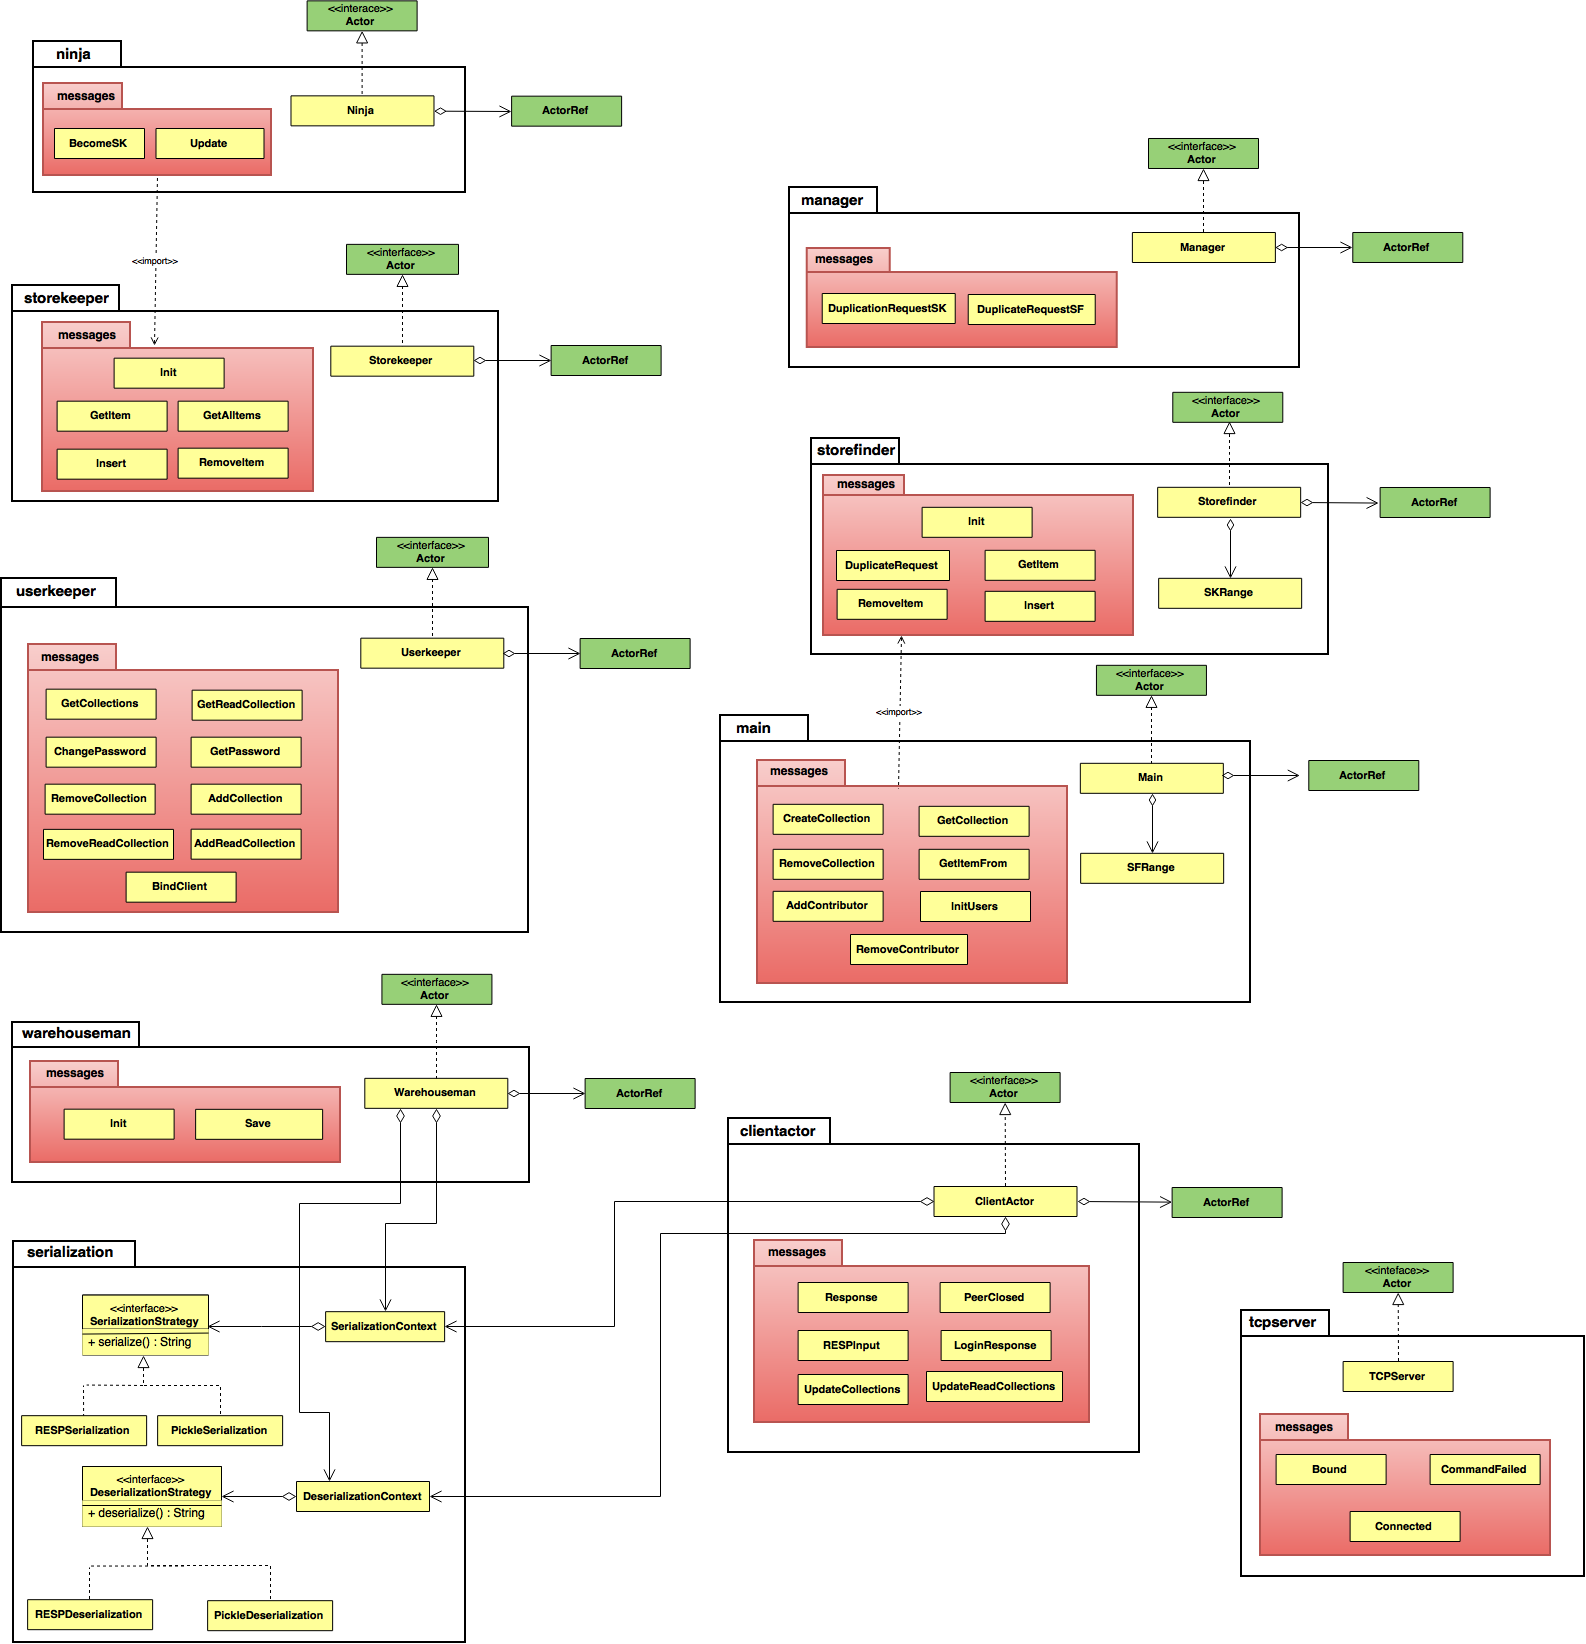
\includegraphics[width=0.9\textwidth,keepaspectratio]{RQ/Actorsystem.png}
    \caption{Actorsystem, visione generale}
  \end{center}
\end{figure}

\subsubsection{Descrizione}

\gloss{Package} che raggruppa tutte le componenti del sistema che
rappresentano il \gloss{server}.

\subsubsection{Package contenuti}

\begin{itemize}
\item \hyperref[sec:actorbase::actorsystem::clientactor]{actorbase::actorsystem::clientactor};
\item \hyperref[sec:actorbase::actorsystem::httpserver]{actorbase::actorsystem::httpserver};
\item \hyperref[sec:actorbase::actorsystem::storefinder]{actorbase::actorsystem::storefinder};
\item \hyperref[sec:actorbase::actorsystem::storekeeper]{actorbase::actorsystem::storekeeper};
\item \hyperref[sec:actorbase::actorsystem::userfinder]{actorbase::actorsystem::userfinder};
\item \hyperref[sec:actorbase::actorsystem::userkeeper]{actorbase::actorsystem::userkeeper};
\item \hyperref[sec:actorbase::actorsystem::warehouseman]{actorbase::actorsystem::warehouseman};
\item \hyperref[sec:actorbase::actorsystem::manager]{actorbase::actorsystem::manager};
\item \hyperref[sec:actorbase::actorsystem::main]{actorbase::actorsystem::main};
\item \hyperref[sec:actorbase::actorsystem::utils]{actorbase::actorsystem::utils}.
\end{itemize}

\subsection{actorbase::actorsystem::utils}
\label{sec:actorbase::actorsystem::utils}

\begin{figure}[H] %TODO aggiungere immagine
  \begin{center}
    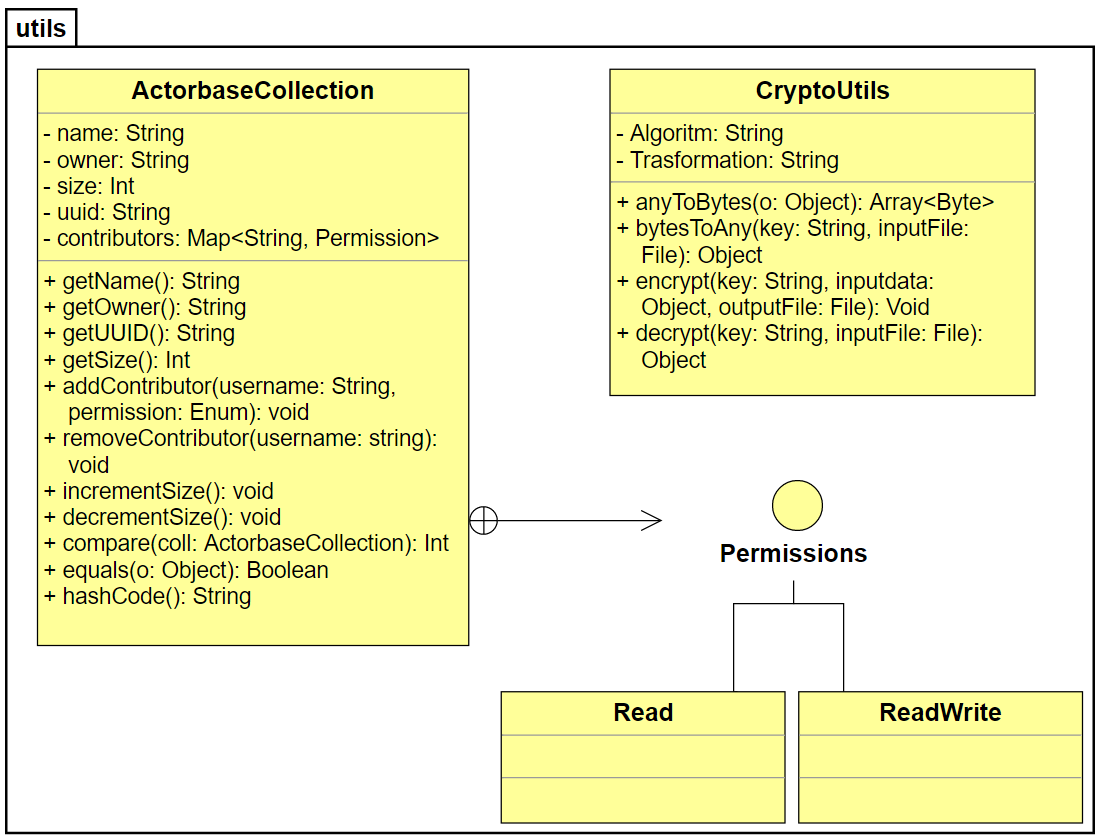
\includegraphics[width=1.0\textwidth,keepaspectratio]{RQ/utils.png}
    \caption{Package actorsystem::utils}
  \end{center}
\end{figure}

\subsubsection{Descrizione}
\gloss{Package} contenente diverse classi di utilità.

\subsubsection{Classi}

%%%%%%%%%%%%%%%%%%%%%%%%%%%%%%%%%%%%%%%%%%%%%%%%%%%%%%%%%%%%%%%%%%%%%%%%%
%%%%%%%%%%%%%%%%%%%%%%%%%%%%%%%%%%%%%%%%%%%%%%%%%%%%%%%%%%%%%%%%%%%%%%%%%

\paragraph{KeyRange}
\label{sec:actorbase::actorsystem::utils::KeyRange}

\subparagraph{Descrizione}
Classe atta a modellare un intervallo di chiavi.\\Viene utilizzata da diversi
attori.

\subparagraph{Utilizzo}
Viene utilizzata da diversi attori del sistema. Questa classe espone metodi
getter, un metodo compare e un metodo per controllare se una determinata
stringa fa parte di questo intervallo di chiavi.

\subparagraph{Realizza}
\begin{itemize}
\item trait scala.math.Ordered.orderingToOrdered
\end{itemize}

\subparagraph{Attributi}
\begin{tabular}{| p{3cm} | p{1.5cm} | p{2cm} | p{2cm} | p{8.5cm} |}
  \hline
  Nome & Accesso & Mutabilità & Tipo & Descrizione\\
  \hline
  minRange & privata & immutabile & String & Rappresenta il limite inferiore delle possibili chiavi di questo range \\
  \hline
  maxRange & private & immutabile & String & Rappresenta il limite superiore delle possibili chiavi di questo range \\
  \hline
\end{tabular}

\subparagraph{Metodi}
\begin{tabular}{| p{3cm} | p{1.5cm} | p{3.5cm} | p{9cm} |}
  \hline
  Nome & Accesso & Tipo di ritorno & Descrizione\\
  \hline
  getMinRange & pubblico & String & Metodo che ritorna il limite minimo del range \\
  \hline
  getMaxRange & pubblico & String & Metodo che ritorna il limite massimo del range \\
  \hline
  contains & pubblico & Boolean & Metodo che ritorna true se il parametro è una stringa contenuta nel KeyRange, false altrimenti\\
  \hline
  toString & pubblico & String & Metodo che ritorna una stringa che contiene un indicazione con il range minimo e massimo del range\\
  \hline
  compare & pubblico & Int & Metodo per l'implementazione dell'interfaccia Ordered\\
  \hline
\end{tabular}

\subparagraph{Parametri}
\begin{center}
  \textbf{contains}\\
\end{center}
\begin{tabular}{| l | l | l |}
  \hline
  Nome & Tipo & Descrizione\\
  \hline
  key & String & Stringa che rappresenta la chiave da controllare se fa parte di questo KeyRange \\
  \hline
\end{tabular}

\begin{center}
  \textbf{compare}\\
\end{center}
\begin{tabular}{| l | l | l |}
  \hline
  Nome & Tipo & Descrizione\\
  \hline
  that & KeyRange & KeyRange da confrontare con l'oggetto this \\
  \hline
\end{tabular}

%%%%%%%%%%%%%%%%%%%%%%%%%%%%%%%%%%%%%%%%%%%%%%%%%%%%%%%%%%%%%%%%%%%%%%%%%
%%%%%%%%%%%%%%%%%%%%%%%%%%%%%%%%%%%%%%%%%%%%%%%%%%%%%%%%%%%%%%%%%%%%%%%%%

\paragraph{CollectionRange}
\label{sec:actorbase::actorsystem::utils::CollectionRange}

\subparagraph{Descrizione}
Classe atta a modellare un intervallo di chiavi di una specifica collezione.

\subparagraph{Utilizzo}
Viene utilizzata da diversi attori del sistema. Questa classe espone metodi
getter, un metodo per il confronto della collezione, un meotodo per il
confronto del range delle chiavi e un metodo compare.

\subparagraph{Realizza}
\begin{itemize}
\item trait scala.math.Ordered.orderingToOrdered
\end{itemize}

\subparagraph{Attributi}
\begin{tabular}{| p{1.5cm} | p{1.5cm} | p{2cm} | p{3.5cm} | p{8.5cm} |}
  \hline
  Nome & Accesso & Mutabilità & Tipo & Descrizione\\
  \hline
  collection & privata & mutabile & \hyperref[sec:actorbase::actorsystem::utils::ActorbaseCollection]{ActorbaseCollection} & Rappresenta la collezione rappresentata \\
  \hline
  range & private & mutabile & \hyperref[sec:actorbase::actorsystem::utils::KeyRange]{KeyRange} & Rappresenta il range di chiavi della collezione \\
  \hline
\end{tabular}

\subparagraph{Metodi}
\begin{tabular}{| p{3cm} | p{1.5cm} | p{3.5cm} | p{9cm} |}
  \hline
  Nome & Accesso & Tipo di ritorno & Descrizione\\
  \hline
  getCollection & pubblico & \hyperref[sec:actorbase::actorsystem::utils::ActorbaseCollection]{ActorbaseCollection} & Metodo che ritorna la collezione rappresentata \\
  \hline
  getKeyRange & pubblico & \hyperref[sec:actorbase::actorsystem::utils::KeyRange]{KeyRange} & Metodo che ritorna il range di chiavi rappresentato \\
  \hline
  contains & pubblico & Boolean & Metodo che ritorna true se il parametro è una stringa contenuta nel KeyRange, false altrimenti\\
  \hline
  isSameCollection & pubblico & Boolean & Metodo che ritorna true se il parametro rappresenta la stessa collezione dell'oggetto this, false altrimenti \\
  \hline
  compare & pubblico & Int & Metodo per l'implementazione dell'interfaccia Ordered \\
  \hline
\end{tabular}

\subparagraph{Parametri}
\begin{center}
  \textbf{contains}\\
\end{center}
\begin{tabular}{| p{1.5cm} | p{1.5cm} | p{9cm} |}
  \hline
  Nome & Tipo & Descrizione\\
  \hline
  key & String & Stringa che rappresenta la chiave da controllare se fa parte del KeyRange della collezione rappresentata \\
  \hline
\end{tabular}

\subparagraph{Parametri}
\begin{center}
  \textbf{isSameCollection}\\
\end{center}
\begin{tabular}{| l | l | l |}
  \hline
  Nome & Tipo & Descrizione\\
  \hline
  that & \hyperref[sec:actorbase::actorsystem::utils::ActorbaseCollection]{ActorbaseCollection} & Collezione da confrontare con la collezione rappresentata dall'oggetto this \\
  \hline
\end{tabular}

\begin{center}
  \textbf{compare}\\
\end{center}
\begin{tabular}{| l | l | l |}
  \hline
  Nome & Tipo & Descrizione\\
  \hline
  that & CollectionRange & CollectionRange da confrontare con l'oggetto this \\
  \hline
\end{tabular}

%%%%%%%%%%%%%%%%%%%%%%%%%%%%%%%%%%%%%%%%%%%%%%%%%%%%%%%%%%%%%%%%%%%%%%%%%
%%%%%%%%%%%%%%%%%%%%%%%%%%%%%%%%%%%%%%%%%%%%%%%%%%%%%%%%%%%%%%%%%%%%%%%%%

\paragraph{CryptoUtils}
\label{sec:actorbase::actorsystem::utils::CryptoUtils}

\subparagraph{Descrizione}
Classe atta a criptare e decriptare i dati per il salvataggio e la lettura dei dati su disco.

\subparagraph{Utilizzo}
Viene utilizzata dall'attore di tipo \gloss{Warehouseman} per il salvataggio e la lettura del database su disco.

\subparagraph{Attributi}
\begin{tabular}{| p{3cm} | p{1.5cm} | p{2cm} | p{2cm} | p{8.5cm} |}
  \hline
  Nome & Accesso & Mutabilità & Tipo & Descrizione\\
  \hline
  Algorithm & pubblica & immutabile & String & Rappresenta l'agoritmo usato per la criptazione \\
  \hline
  Transformation & pubblica & immutabile & String & Rappresenta la trasformazione per ottenere il cifrario usato per la criptazione \\
  \hline
\end{tabular}

\subparagraph{Metodi} %TODO sfora
\begin{tabular}{| p{3cm} | p{1.5cm} | p{3.5cm} | p{9cm} |}
  \hline
  Nome & Accesso & Tipo di ritorno & Descrizione\\
  \hline
  encrypt & pubblico & Unit & Metodo che si occupa di criptare i dati \\
  \hline
  decrypt & pubblico & TreeMap[String, Any] & Metodo che si occupa di decriptare i dati \\
  \hline
\end{tabular}

\subparagraph{Parametri}
\begin{center}
  \textbf{encrypt}\\
\end{center}
\begin{tabular}{| l | l | l |}
  \hline
  Nome & Tipo & Descrizione\\
  \hline
  key & String & Stringa che rappresenta la chiave di criptazione \\
  \hline
  inputData & TreeMap[String, Any] & Mappa che rappresenta i dati che verranno criptati \\
  \hline
  outputFile & File & File destinato a contenere i dati criptati \\
  \hline
\end{tabular}

\begin{center}
  \textbf{decrypt}\\
\end{center}
\begin{tabular}{| l | l | l |}
  \hline
  Nome & Tipo & Descrizione\\
  \hline
  key & String & Stringa che rappresenta la chiave di decriptazione \\
  \hline
  inputFile & File & File che contiene i dati da decriptare \\
  \hline
\end{tabular}

%%%%%%%%%%%%%%%%%%%%%%%%%%%%%%%%%%%%%%%%%%%%%%%%%%%%%%%%%%%%%%%%%%%%%%%%%%%%%%
%%%%%%%%%%%%%%%%%%%%%%%%%%%%%%%%%%%%%%%%%%%%%%%%%%%%%%%%%%%%%%%%%%%%%%%%%%%%%%

\paragraph{ActorbaseCollection}
\label{sec:actorbase::actorsystem::utils::ActorbaseCollection}

\subparagraph{Descrizione}
Classe atta a modellare una collezione del sistema actorbase.

\subparagraph{Utilizzo}
Viene utilizzata da diversi attori del sistema. Questa classe espone metodi
getter e un meotodo per il confronto con un altro oggetto ActorbaseCollection.

\subparagraph{Realizza}
\begin{itemize}
\item trait scala.math.Ordered
\end{itemize}

\subparagraph{Attributi}
\begin{tabular}{| p{3cm} | p{1.5cm} | p{2cm} | p{2cm} | p{8.5cm} |}
  \hline
  Nome & Accesso & Mutabilità & Tipo & Descrizione\\
  \hline
  name & privata & mutabile & String & Rappresenta il nome della collezione \\
  \hline
  owner & private & mutabile & String & Rappresenta lo username dell'utente che ha creato la collezione \\
  \hline
\end{tabular}

\subparagraph{Metodi}
\begin{tabular}{| l | l | l | l |}
  \hline
  Nome & Accesso & Tipo di ritorno & Descrizione\\
  \hline
  getName & pubblico & String & Metodo che ritorna il nome della collezione \\
  \hline
  getOwner & pubblico & String & Metodo che ritorna lo username dell'utente che ha creato la collezione \\
  \hline
  compare & pubblico & Int & Metodo per l'implementazione dell'interfaccia Ordered.\\
  \hline
\end{tabular}

\begin{center}
  \textbf{compare}\\
\end{center}
\begin{tabular}{| l | l | l |}
  \hline
  Nome & Tipo & Descrizione\\
  \hline
  that & ActorbaseCollection & ActorbaseCollection da confrontare con l'oggetto this \\
  \hline
\end{tabular}

% TODO di utils manca cryptoutils

%%%%%%%%%%%%%%%%%%%%%%%%%%%%%%%%%%%%%%%%%%%%%%%%%%%%%%%%%%%%%%%%%%%%%%%%%
%%%%%%%%%%%%%%%%%%%%%%%%%%%%%%%%%%%%%%%%%%%%%%%%%%%%%%%%%%%%%%%%%%%%%%%%%
%%%%%%%%%%%%%%%%%%%%%%%%%%%%%%%%%%%%%%%%%%%%%%%%%%%%%%%%%%%%%%%%%%%%%%%%%

\subsection{actorbase::actorsystem::clientactor}
\label{sec:actorbase::actorsystem::clientactor}

\begin{figure}[H]
  \begin{center}
    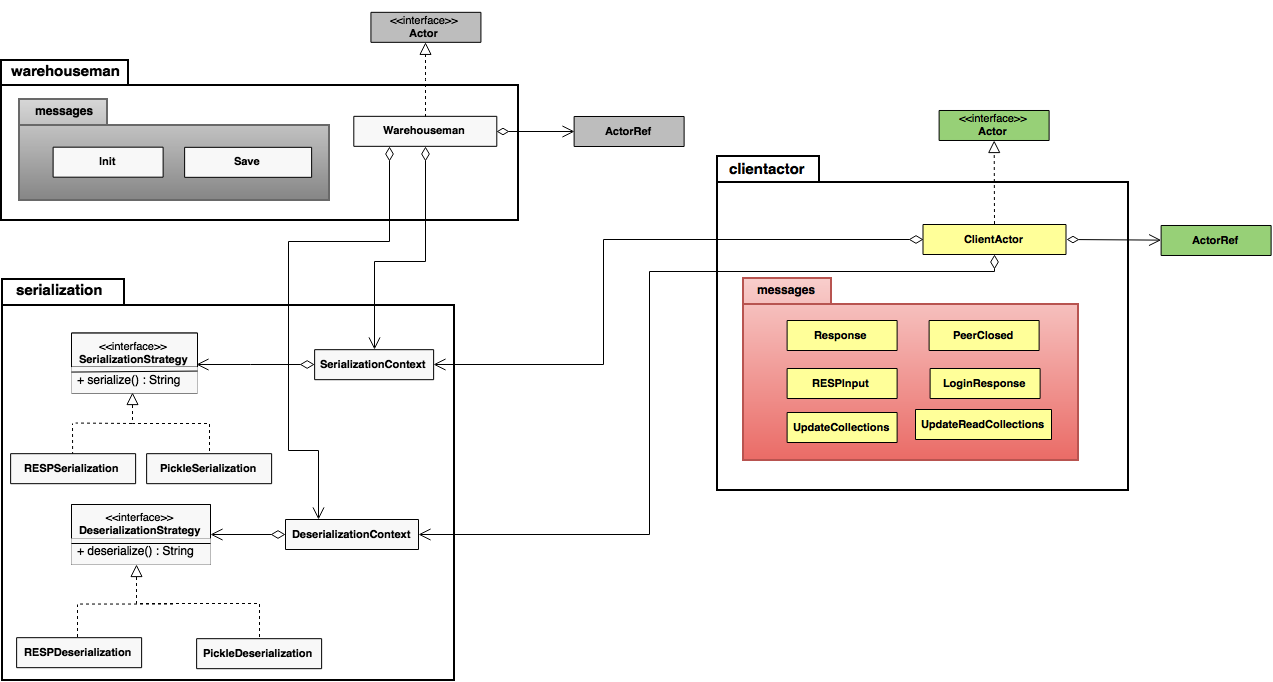
\includegraphics[width=1.0\textwidth,keepaspectratio]{RQ/Clientactor.png}
    \caption{Clientactor e interazioni con main e package serialization}
  \end{center}
\end{figure}

\subsubsection{Descrizione}

\gloss{Package} per l'\gloss{attore} con cui si interfaccerà il \gloss{driver}.

\subsubsection{Package contenuti}

\begin{itemize}
\item \hyperref[sec:actorbase::actorsystem::clientactor::messages]{actorbase::actorsystem::clientactor::messages}.
\end{itemize}

\subsubsection{Classi}

\paragraph{actorbase::actorsystem::clientactor::Authenticator}
\label{sec:actorbase::actorsystem::clientactor::Authenticator}

\subparagraph{Descrizione}

Classe astratta usata per effettuare la validazione di un login.

\subparagraph{Utilizzo}

Questa classe viene usata dalla classe che la realizza per effettuare il controllo
delle credenziali di login.

\subparagraph{Metodi}

\begin{tabular}{| p{4cm} | p{1.5cm} | p{4cm} | p{7.5cm} |}
  \hline
  Nome & Accesso & Tipo di ritorno & Descrizione\\
  \hline
  basicUserAuthenticator & public & AuthMagnet[AuthInfo] & Metodo che riceve e controlla tramite metodi interni le credenziali\\
  \hline
  validateUser & public & Option[AuthInfo] & Metodo che controlla che le credenziali siano corrette\\
  \hline
  authenticator & public & Future[Option[AuthInfo]] & Metodo che restituisce un \gloss{future} che punta alle credenziali dell'utente autenticato\\
  \hline
\end{tabular}

\subparagraph{Parametri}

\begin{center}
  \textbf{basicUserAuthenticator}\\
\end{center}
\begin{tabular}{| p{2cm} | p{3cm} | p{12cm} |}
  \hline
  Nome & Tipo & Descrizione\\
  \hline
  ec & ExecutionContext & Contesto di esecuzione all'interno del quale è stato chiamato questo metodo\\
  \hline
  router & ActorRef & Riferimento dell'attore che si occuperà di comunicare con un attore \gloss{main} per effettuare le operazioni richieste \\
  \hline
\end{tabular}
\\
\begin{center}
  \textbf{validateUser}\\
\end{center}
\begin{tabular}{| l | l | l |}
  \hline
  Nome & Tipo & Descrizione\\
  \hline
  userPass & Option[UserPass] & Credenziali di accesso dell'utente che vuole autenticarsi\\
  \hline
\end{tabular}
\\
\begin{center}
  \textbf{authenticator}\\
\end{center}
\begin{tabular}{| l | l | l |}
  \hline
  Nome & Tipo & Descrizione\\
  \hline
  userPass & Option[UserPass] & Credenziali di accesso dell'utente che vuole autenticarsi\\
  \hline
\end{tabular}

\paragraph{actorbase::actorsystem::clientactor::ItemApi}
\label{sec:actorbase::actorsystem::clientactor::ItemApi}

\subparagraph{Descrizione}

Classe astratta usata per analizzare le route che richiedono operazioni su item.

\subparagraph{Utilizzo}

Questa classe viene usata dalla classe che la realizza per effettuare l'analisi
delle route che richiedono operazioni su item.

\subparagraph{Attributi}
\begin{tabular}{| p{1cm} | p{1.5cm} | p{2cm} | p{4cm} | p{8.5cm} |}
  \hline
  Nome & Accesso & Mutabilità & Tipo & Descrizione\\
  \hline
  ec & public & immutabile & ExecutionContext & Rappresenta il Contesto di esecuzione all'interno del quale è stata creata questa classe \\
  \hline
\end{tabular}

\subparagraph{Metodi}

\begin{tabular}{| p{2.5cm} | p{2.5cm} | p{2.5cm} | p{9.5cm} |}
  \hline
  Nome & Accesso & Tipo di ritorno & Descrizione\\
  \hline
  items & public & Route & Metodo che interagisce con il server tramite un router basandosi sulla route immessa dall'utente\\
  \hline
\end{tabular}

\subparagraph{Parametri}

\begin{center}
  \textbf{items}\\
\end{center}
\begin{tabular}{| p{2.5cm} | p{2.5cm} | p{12cm} |}
  \hline
  Nome & Tipo & Descrizione\\
  \hline
  owner & String & Proprietario della collezione su cui si vuole operare\\
  \hline
  router & ActorRef & Riferimento dell'attore che si occuperà di comunicare con un attore \gloss{main} per effettuare le operazioni richieste\\
  \hline
  collectionName & String & Nome della collezione su cui si vuole operare\\
  \hline
\end{tabular}

\paragraph{actorbase::actorsystem::clientactor::UserApi}
\label{sec:actorbase::actorsystem::clientactor::UserApi}

\subparagraph{Descrizione}

Classe astratta usata per analizzare le route che richiedono operazioni su utenti.

\subparagraph{Utilizzo}

Questa classe viene usata dalla classe che la realizza per effettuare l'analisi
delle route che richiedono operazioni su utenti.

\subparagraph{Attributi}
\begin{tabular}{| p{1.5cm} | p{1.5cm} | p{2cm} | p{3cm} | p{8.5cm} |}
  \hline
  Nome & Accesso & Mutabilità & Tipo & Descrizione\\
  \hline
  ec & public & immutabile & ExecutionContext & Rappresenta il Contesto di esecuzione all'interno del quale è stata creata questa classe \\
  \hline
\end{tabular}

\subparagraph{Metodi}

\begin{tabular}{| p{1.5cm} | p{1.5cm} | p{2.5cm} | p{9.5cm} |}
  \hline
  Nome & Accesso & Tipo di ritorno & Descrizione\\
  \hline
  users & public & Route & Metodo che interagisce con il server tramite un router basandosi sulla route immessa dall'utente\\
  \hline
\end{tabular}

\subparagraph{Parametri}

\begin{center}
  \textbf{collections}\\
\end{center}
\begin{tabular}{| p{2cm} | p{2cm} | p{12.5cm} |}
  \hline
  Nome & Tipo & Descrizione\\
  \hline
  user & String & Utente su cui si vuole operare\\
  \hline
  router & ActorRef & Riferimento dell'attore che si occuperà di comunicare con un attore \gloss{main} per effettuare le operazioni richieste \\
  \hline
\end{tabular}

\paragraph{actorbase::actorsystem::clientactor::CollectionApi}
\label{sec:actorbase::actorsystem::clientactor::CollectionApi}

\subparagraph{Descrizione}

Classe astratta usata per analizzare le route che richiedono operazioni su collezioni.

\subparagraph{Utilizzo}

Questa classe viene usata dalla classe che la realizza per effettuare l'analisi
delle route che richiedono operazioni su collezioni.

\subparagraph{Attributi}
\begin{tabular}{| p{2cm} | p{1.5cm} | p{2cm} | p{3cm} | p{8.5cm} |}
  \hline
  Nome & Accesso & Mutabilità & Tipo & Descrizione\\
  \hline
  ec & public & immutabile & ExecutionContext & Rappresenta il Contesto di esecuzione all'interno del quale è stata creata questa classe \\
  \hline
\end{tabular}

\subparagraph{Metodi}

\begin{tabular}{| p{2cm} | p{1.5cm} | p{2.5cm} | p{11.5cm} |}
  \hline
  Nome & Accesso & Tipo di ritorno & Descrizione\\
  \hline
  collections & public & Route & Metodo che interagisce con il server tramite un router basandosi sulla route immessa dall'utente\\
  \hline
\end{tabular}

\subparagraph{Parametri}

\begin{center}
  \textbf{collections}\\
\end{center}
\begin{tabular}{| p{1.5cm} | p{1.5cm} | p{14cm} |}
  \hline
  Nome & Tipo & Descrizione\\
  \hline
  owner & String & Proprietario della collezione su cui si vuole operare\\
  \hline
  router & ActorRef & Riferimento dell'attore che si occuperà di comunicare con un attore \gloss{main} per effettuare le operazioni richieste\\
  \hline
\end{tabular}

\paragraph{actorbase::actorsystem::clientactor::ClientActor} %TODO da fare
\label{sec:actorbase::actorsystem::clientactor::ClientActor}

\subparagraph{Descrizione}

Classe che rappresenta l'\gloss{attore} con cui si interfaccia il \gloss{driver} dopo
la connessione.

\subparagraph{Utilizzo}

Questo \gloss{attore} riceve le richieste da \hyperref[sec:actorbase::driver::client::Connection]{actorbase::driver::client::Connection}
e si occupa di inviare messaggi a \hyperref[sec:actorbase::actorsystem::main::Main]{actorbase::actorsystem::main::Main}. \\
Questa classe inoltre si occupa di capire che tipo di richiesta è stata fatta dal \gloss{driver} basandosi sulla route di quest'ultima.

\subparagraph{Classi ereditate}

\begin{itemize}

\item akka::actor::Actor;
\item \hyperref[com::actorbase::actorsystem::clientactor::Authenticator]{com::actorbase::actorsystem::clientactor::Authenticator};
\item \hyperref[com::actorbase::actorsystem::clientactor::CollectionApi]{com::actorbase::actorsystem::clientactor::CollectionApi};
\item \hyperref[com::actorbase::actorsystem::clientactor::RestApi]{com::actorbase::actorsystem::clientactor::RestApi};.

\end{itemize}

\subparagraph{Attributi}
\begin{tabular}{| p{3cm} | p{1.5cm} | p{2cm} | p{3cm} | p{7.5cm} |}
  \hline
  Nome & Accesso & Mutabilità & Tipo & Descrizione\\
  \hline
  router & public & immutabile & ActorRef & Rappresenta il riferimento di un attore che si occuperà di gestire le richieste verso i vari \gloss{main} \\
  \hline
  timeout & public & immutabile & Timeout & Rappresenta il tempo limite oltre il quale se un'operazione non è conclusa viene lanciato un errore di timeout \\
  \hline
  collections & private & mutabile & ListBuffer[String] & Rappresenta la lista di collezioni a cui l'utente ha accesso in scrittura e lettura \\
  \hline
  readCollections & private & mutabile & ListBuffer[String] & Rappresenta la lista di collezioni a cui l'utente ha accesso in sola lettura \\
  \hline
\end{tabular}

\subparagraph{Metodi}

\begin{tabular}{| l | l | l | l |}
  \hline
  Nome & Accesso & Tipo di ritorno & Descrizione\\
  \hline
  receive & public &  & Effettua operazioni diverse a seconda del tipo di messaggio ricevuto\\
  \hline
\end{tabular}

\subsection{actorbase::actorsystem::clientactor::messages}
\label{sec:actorbase::actorsystem::clientactor::messages}

\subsubsection{Descrizione}

\gloss{Package} che contiene tutti i messaggi che possono essere ricevuti da
\hyperref[sec:actorbase::actorsystem::clientactor::ClientActor]{actorbase::actorsystem::clientactor::ClientActor}.

\subsubsection{Classi}

\paragraph{actorbase::actorsystem::clientactor::messages::Response}
\label{sec:actorbase::actorsystem::clientactor::messages::Response}

\subparagraph{Descrizione}

Messaggio che rappresenta la risposta da parte del \gloss{server} da inoltrare
al \gloss{driver}.

\subparagraph{Utilizzo}

Quando \hyperref[sec:actorbase::actorsystem::clientactor::ClientActor]{actorbase::actorsystem::clientactor::ClientActor}
riceve questo messaggio il contenuto di quest'ultimo viene
mandato a \hyperref[sec:actorbase::driver::client::ActorbaseClient]{actorbase::driver::\allowbreak{}client::\allowbreak{}ActorbaseClient}.

\subparagraph{Attributi}
\begin{tabular}{| p{3cm} | p{1.5cm} | p{2cm} | p{2cm} | p{8.5cm} |}
  \hline
  Nome & Accesso & Mutabilità & Tipo & Descrizione\\
  \hline
  response & public & immutabile & String & Rappresenta la risposta ricevuta dal server \\
  \hline
\end{tabular}

\paragraph{actorbase::actorsystem::clientactor::messages::MapResponse}
\label{sec:actorbase::actorsystem::clientactor::messages::MapResponse}

\subparagraph{Descrizione}

Messaggio che rappresenta la risposta da parte del \gloss{server} ad una ricerca da inoltrare
al \gloss{driver}.

\subparagraph{Utilizzo}

Quando \hyperref[sec:actorbase::actorsystem::clientactor::ClientActor]{actorbase::actorsystem::clientactor::ClientActor}
riceve questo messaggio il contenuto di quest'ultimo viene
mandato a \hyperref[sec:actorbase::driver::client::ActorbaseClient]{actorbase::driver::\allowbreak{}client::\allowbreak{}ActorbaseClient}.

\subparagraph{Attributi}
\begin{tabular}{| p{1.5cm} | p{1.5cm} | p{2cm} | p{3.5cm} | p{8.5cm} |}
  \hline
  Nome & Accesso & Mutabilità & Tipo & Descrizione\\
  \hline
  collection & public & immutabile & String & Rappresenta la collezione su cui è stata fatta la ricerca \\
  \hline
  map & public & immutabile & Map[String, Any] & Rappresenta l'item (o l'insieme di item) cercati \\
  \hline
\end{tabular}

%%%%%%%%%%%%%%%%%%%%%%%%%%%%%%%%%%%%%%%%%%%%%%%%%%%%%%%%%%%%%%%%%%%%%%%%%
%%%%%%%%%%%%%%%%%%%%%%%%%%%%%%%%%%%%%%%%%%%%%%%%%%%%%%%%%%%%%%%%%%%%%%%%%
%%%%%%%%%%%%%%%%%%%%%%%%%%%%%%%%%%%%%%%%%%%%%%%%%%%%%%%%%%%%%%%%%%%%%%%%%

\subsection{actorbase::actorsystem::httpserver} %TODO da ricontrollare
\label{sec:actorbase::actorsystem::httpserver}

\begin{figure}[H]
  \begin{center}
    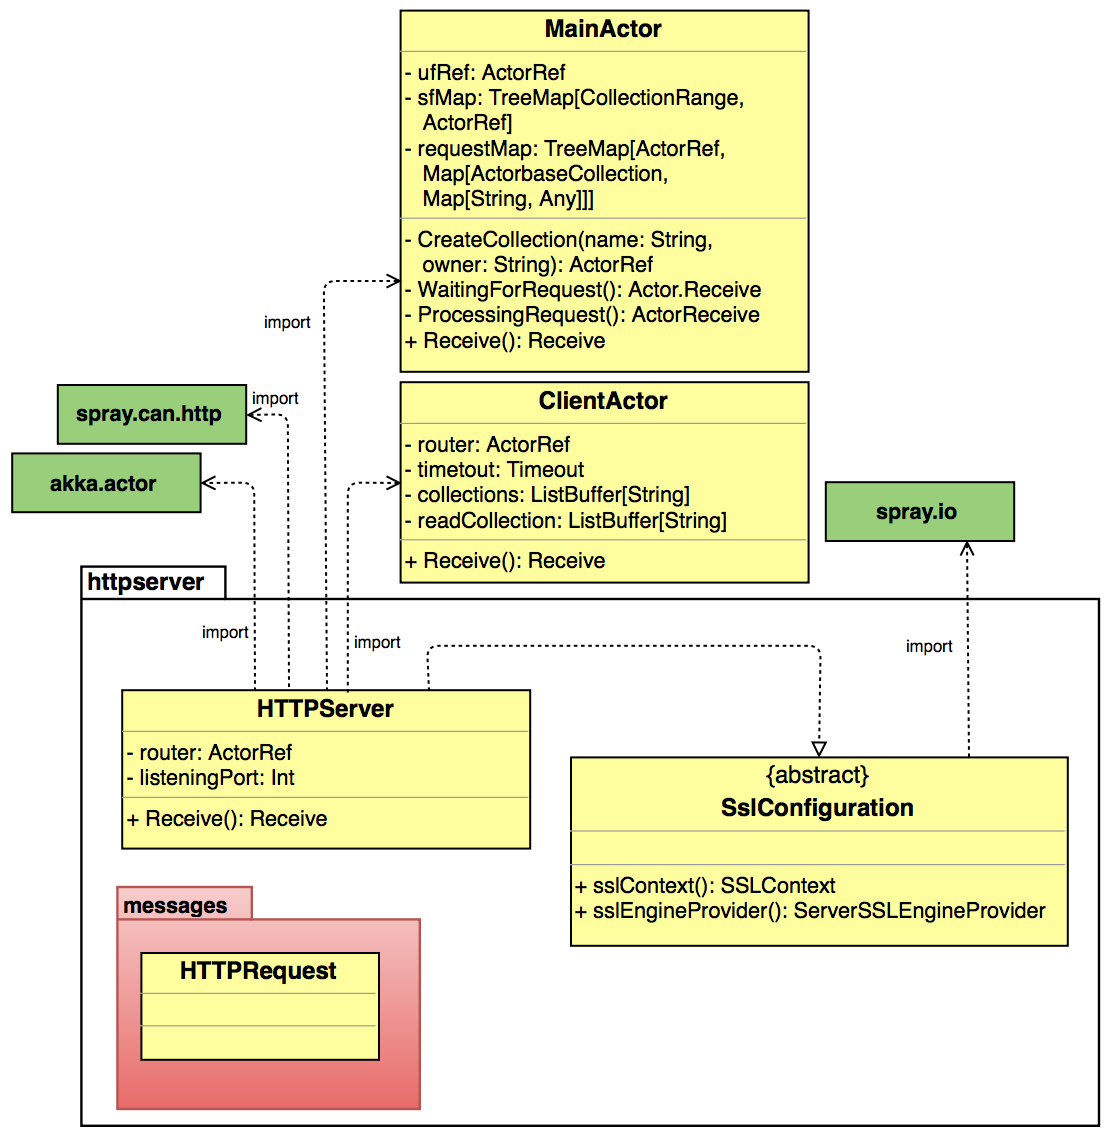
\includegraphics[width=0.5\textwidth,keepaspectratio]{RQ/httpserver.png} % TODO IMMAGINE DA INSERIRE E DA CREARE PERCHE' E' BELLO COSì
    \caption{httpserver, visione generale del package}
  \end{center}
\end{figure}

\subsubsection{Descrizione}
\gloss{Package} per l'\gloss{attore} con cui si interfaccerà il \gloss{driver} per la connessione iniziale.

\subsubsection{Package contenuti}
\begin{itemize}
\item \hyperref[sec:actorbase::actorsystem::httpserver::messages]{actorbase::actorsystem::httpserver::messages}.
\end{itemize}

\subsubsection{Classi}

\paragraph{actorbase::actorsystem::httpserver::HTTPServer}
\label{sec:actorbase::actorsystem::httpserver::HTTPServer}

\subparagraph{Descrizione}
Classe che rappresenta l'\gloss{attore} con cui si interfaccia il \gloss{driver} per
istanziare la connessione.

\subparagraph{Utilizzo}

Questo \gloss{attore} riceve la richiesta di connessione da
\hyperref[sec:actorbase::driver::client::ActorbaseClient]{ActorbaseClient}
e si occupa di associare al \gloss{client} un \gloss{attore} di tipo
\hyperref[sec:actorbase::actorsystem::clientactor::ClientActor]{ClientActor}
per continuare le comunicazioni.

\subparagraph{Classi ereditate}
\begin{itemize}
\item akka::actor::Actor.
\end{itemize}

\subparagraph{Attributi}
\begin{tabular}{| p{3cm} | p{1.5cm} | p{2cm} | p{2cm} | p{8.5cm} |}
  \hline
  Nome & Accesso & Mutabilità & Tipo & Descrizione\\
  \hline
  router & privata & immutabile & ActorRef & Rappresenta un riferimento all'attore che si occupa del routing delle richieste agli attori di tipo \hyperref[sec:actorbase::actorsystem::main::Main]{Main} \\
  \hline
  listenPort & private & immutabile & Int & Rappresenta la porta in cui il server si mette in ascolto \\
  \hline
\end{tabular}

\subparagraph{Metodi}

\begin{tabular}{| l | l | l | l |}
  \hline
  Nome & Accesso & Tipo di ritorno & Descrizione\\
  \hline
  receive & public &  & Effettua operazioni diverse a seconda del tipo di messaggio ricevuto\\
  \hline
\end{tabular}

\paragraph{actorbase::actorsystem::httpserver::SslConfiguration}
\label{sec:actorbase::actorsystem::httpserver::SslConfiguration}

\subparagraph{Descrizione}
Classe che contiene metodi di utilità per applicare algoritmi di crittografia
ssl.

\subparagraph{Metodi}

\begin{tabular}{| l | l | l | l |}
  \hline
  Nome & Accesso & Tipo di ritorno & Descrizione\\
  \hline
  sslContext & public & SSLContext & metodo per impostare le opzioni per SSL\\
  \hline
  sslEngineProvider & public & ServerSSLEngineProvider & metodo per impostare una \gloss{cipher suite}\\
  \hline
\end{tabular}

%%%%%%%%%%%%%%%%%%%%%%%%%%%%%%%%%%%%%%%%%%%%%%%%%%%%%%%%%%%%%%%%%%%%%%%%%
%%%%%%%%%%%%%%%%%%%%%%%%%%%%%%%%%%%%%%%%%%%%%%%%%%%%%%%%%%%%%%%%%%%%%%%%%
%%%%%%%%%%%%%%%%%%%%%%%%%%%%%%%%%%%%%%%%%%%%%%%%%%%%%%%%%%%%%%%%%%%%%%%%%

\subsection{actorbase::actorsystem::warehouseman} %TODO DA FARE
\label{sec:actorbase::actorsystem::warehouseman}

\begin{figure}[H]
  \begin{center}
    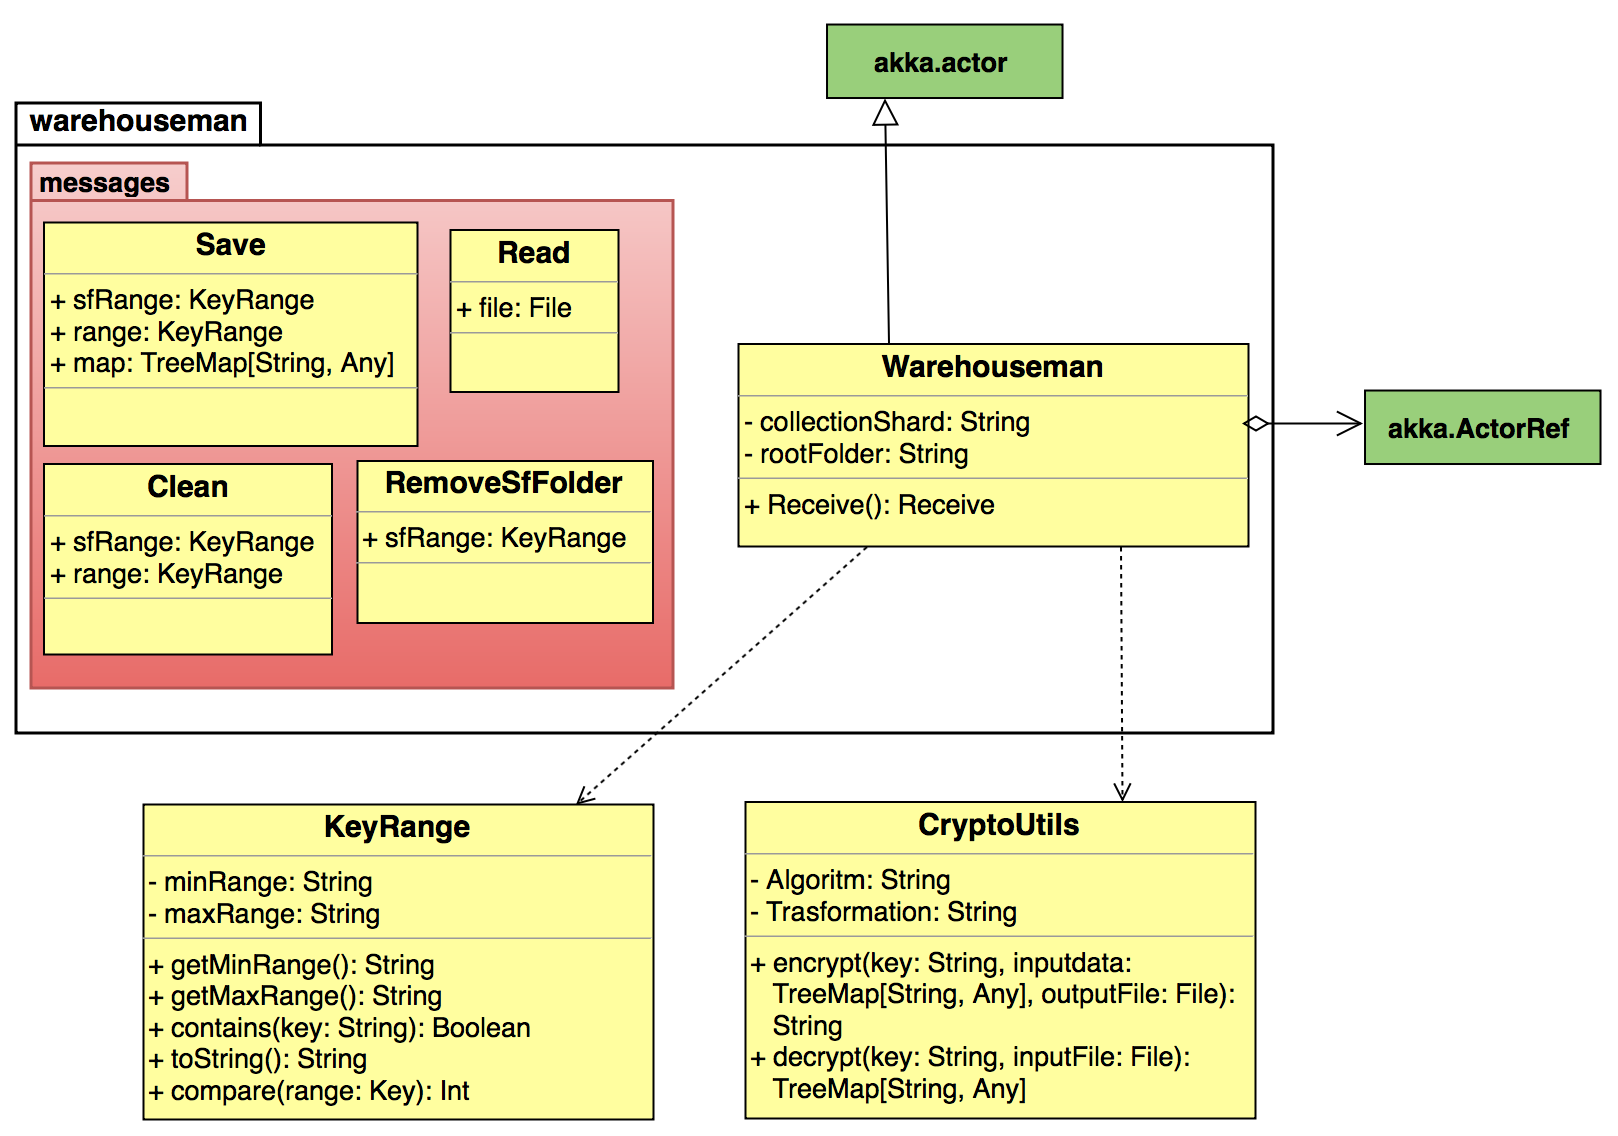
\includegraphics[width=1.0\textwidth,keepaspectratio]{RQ/Warehouseman.png}
    \caption{Warehouseman e interazioni con main e serialization}
  \end{center}
\end{figure}

\subsubsection{Descrizione}

\gloss{Package} che rappresenta l'\gloss{attore} che si occuperà della
\gloss{persistenza} su disco dei dati.

\subsubsection{Package contenuti}

\begin{itemize}

\item \hyperref[sec:actorbase::actorsystem::warehouseman::messages]{actorbase::actorsystem::warehouseman::messages}.

\end{itemize}

\subsubsection{Classi}

\paragraph{actorbase::actorsystem::warehouseman::Warehouseman}
\label{sec:actorbase::actorsystem::warehouseman::Warehouseman}

\subparagraph{Descrizione}

Classe che rappresenta un \gloss{attore} di tipo \gloss{Warehouseman}.

\subparagraph{Utilizzo}

Questa classe viene utilizzata per effettuare il salvataggio su filesystem del
\gloss{database} e per caricare i dati da filesystem.

\subparagraph{Classi ereditate}

\begin{itemize}

\item akka::actor::Actor.

\end{itemize}

\subparagraph{Attributi}
\begin{tabular}{| p{3cm} | p{1.5cm} | p{2cm} | p{2cm} | p{8.5cm} |}
  \hline
  Nome & Accesso & Mutabilità & Tipo & Descrizione\\
  \hline
  collectionShard & pubblico & immutabile & String & Rappresenta il nome della cartella dentro cui verranno salvati i dati \\
  \hline
\end{tabular}

\subparagraph{Metodi}
\begin{tabular}{| l | l | l | l |}
  \hline
  Nome & Accesso & Tipo di ritorno & Descrizione\\
  \hline
  receive & pubblico & Unit & Effettua operazioni diverse a seconda del tipo di messaggio ricevuto \\
  \hline
  removeAll & privato & Unit & Rimuove tutti i file all'interno di una cartella, eliminando anche quest'ultima \\
  \hline
\end{tabular}

\subparagraph{Parametri}

\begin{center}
  \textbf{removeAll}\\
\end{center}
\begin{tabular}{| l | l | l |}
  \hline
  Nome & Tipo & Descrizione\\
  \hline
  path & String & Percorso della cartella da eliminare\\
  \hline
\end{tabular}

\subsection{actorbase::actorsystem::warehouseman::messages}
\label{sec:actorbase::actorsystem::warehouseman::messages}

\subsubsection{Descrizione}

\gloss{Package} che racchiude tutti i messaggi che gli attori di tipo
\gloss{Warehouseman} possono ricevere.

\paragraph{actorbase::actorsystem::warehouseman::messages::Save}
\label{sec:actorbase::actorsystem::warehouseman::messages::Save}

\subparagraph{Descrizione}

Messaggio che porta al salvataggio dei dati su disco.

\subparagraph{Utilizzo}

Quando \hyperref[sec:actorbase::actorsystem::warehouseman::Warehouseman]{actorbase::actorsystem::warehouseman::Warehouseman}
riceve questo messaggio salverà i dati su disco sfruttando
\hyperref[sec:actorbase::actorsystem::utils::CryptoUtils]{actorbase::actorsystem::utils::CryptoUtils}.

\subparagraph{Attributi}
\begin{tabular}{| p{1.5cm} | p{1.5cm} | p{2cm} | p{3.5cm} | p{8.5cm} |}
  \hline
  Nome & Accesso & Mutabilità & Tipo & Descrizione\\
  \hline
  sfRange & pubblico & immutabile & KeyRange & Rappresenta il \gloss{collectionShard} identificativo del padre dell'attore che ha richiesto il salvataggio \\
  \hline
  range & pubblico & immutabile & KeyRange & Rappresenta il \gloss{collectionShard} che verrà salvato \\
  \hline
  map & pubblico & immutabile & TreeMap[String, Any] & Rappresenta i dati che verranno salvati \\
  \hline
\end{tabular}

\paragraph{actorbase::actorsystem::warehouseman::messages::Clean}
\label{sec:actorbase::actorsystem::warehouseman::messages::Clean}

\subparagraph{Descrizione}

Messaggio che porta alla cancellazione dal filesystem di alcuni dati.

\subparagraph{Utilizzo}

Quando \hyperref[sec:actorbase::actorsystem::warehouseman::Warehouseman]{actorbase::actorsystem::warehouseman::Warehouseman}
riceve questo messaggio rimuoverà i dati dal filesystem.

\subparagraph{Attributi}
\begin{tabular}{| p{3cm} | p{1.5cm} | p{2cm} | p{2cm} | p{8.5cm} |}
  \hline
  Nome & Accesso & Mutabilità & Tipo & Descrizione\\
  \hline
  sfRange & pubblico & immutabile & KeyRange & Rappresenta il \gloss{collectionShard} identificativo del padre dell'attore che ha richiesto la rimozione \\
  \hline
  range & pubblico & immutabile & KeyRange & Rappresenta il \gloss{collectionShard} che verrà rimosso \\
  \hline
\end{tabular}

\paragraph{actorbase::actorsystem::warehouseman::messages::RemoveSfFolder}
\label{sec:actorbase::actorsystem::warehouseman::messages::RemoveSfFolder}

\subparagraph{Descrizione}

Messaggio che porta alla rimozione di una cartella da disco.

\subparagraph{Utilizzo}

Quando \hyperref[sec:actorbase::actorsystem::warehouseman::Warehouseman]{actorbase::actorsystem::warehouseman::Warehouseman}
riceve questo messaggio rimuoverà i dati da disco.

\subparagraph{Attributi}
\begin{tabular}{| p{3cm} | p{1.5cm} | p{2cm} | p{2cm} | p{8.5cm} |}
  \hline
  Nome & Accesso & Mutabilità & Tipo & Descrizione\\
  \hline
  sfRange & pubblico & immutabile & KeyRange & Rappresenta il \gloss{collectionShard} identificativo dei dati da rimuovere \\
  \hline
\end{tabular}

\paragraph{actorbase::actorsystem::warehouseman::messages::Read}
\label{sec:actorbase::actorsystem::warehouseman::messages::Read}

\subparagraph{Descrizione}

Messaggio che porta alla lettura di dati da disco.

\subparagraph{Utilizzo}

Quando \hyperref[sec:actorbase::actorsystem::warehouseman::Warehouseman]{actorbase::actorsystem::warehouseman::Warehouseman}
riceve questo messaggio leggerà i dati da disco sfruttando
\hyperref[sec:actorbase::actorsystem::utils::CryptoUtils]{actorbase::actorsystem::utils::CryptoUtils}.

\subparagraph{Attributi}
\begin{tabular}{| p{3cm} | p{1.5cm} | p{2cm} | p{2cm} | p{8.5cm} |}
  \hline
  Nome & Accesso & Mutabilità & Tipo & Descrizione\\
  \hline
  file & pubblico & immutabile & File & Rappresenta il file che verrà letto \\
  \hline
\end{tabular}

%%%%%%%%%%%%%%%%%%%%%%%%%%%%%%%%%%%%%%%%%%%%%%%%%%%%%%%%%%%%%%%%%%%%%%%%%
%%%%%%%%%%%%%%%%%%%%%%%%%%%%%%%%%%%%%%%%%%%%%%%%%%%%%%%%%%%%%%%%%%%%%%%%%
%%%%%%%%%%%%%%%%%%%%%%%%%%%%%%%%%%%%%%%%%%%%%%%%%%%%%%%%%%%%%%%%%%%%%%%%%

\subsection{actorbase::actorsystem::main} %TODO DA controllare e finire
\label{sec:actorbase::actorsystem::main}

\begin{figure}[H]
  \begin{center}
    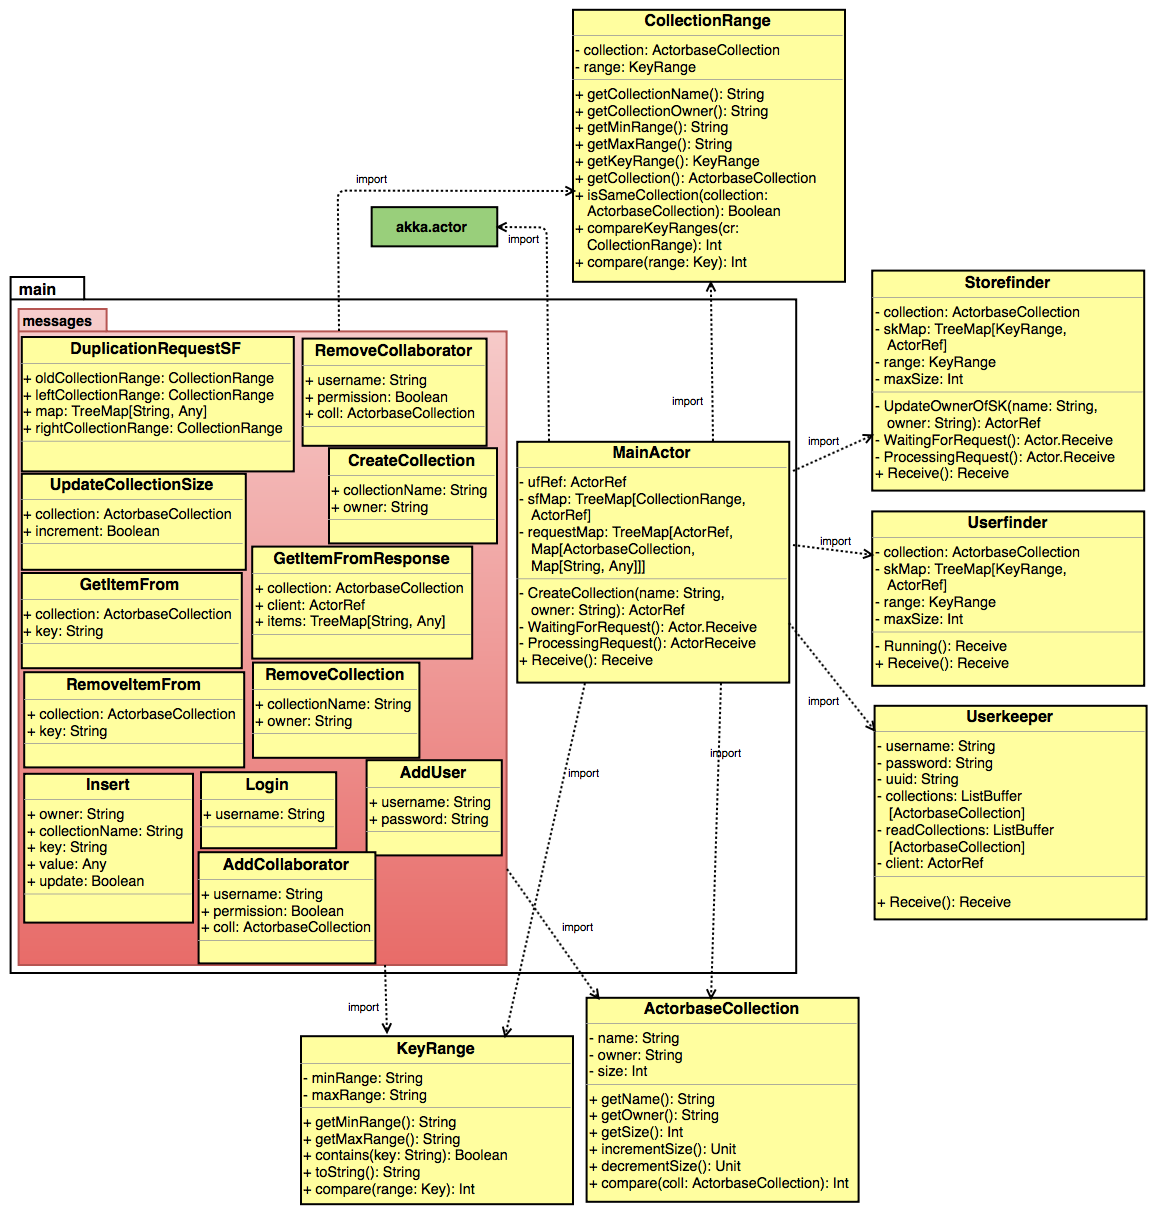
\includegraphics[width=0.8\textwidth,keepaspectratio]{RQ/Main.png}
    \caption{Package dell'attore di tipo Main}
  \end{center}
\end{figure}

\subsubsection{Descrizione}
\gloss{Package} che rappresenta l'\gloss{attore} che si occuperà di gestire le
richieste al \gloss{server}.

\subsubsection{Package contenuti}
\begin{itemize}
\item \hyperref[sec:actorbase::actorsystem::main::messages]{actorbase::actorsystem::main::messages}.
\end{itemize}

\subsubsection{Classi}

\paragraph{actorbase::actorsystem::main::Main}
\label{sec:actorbase::actorsystem::main::Main}

\subparagraph{Descrizione}
Classe che rappresenta un \gloss{attore} di tipo \gloss{Main}.

\subparagraph{Utilizzo}
Questa classe viene utilizzata per gestire le richieste ricevute al
\gloss{server}.

\subparagraph{Classi ereditate}
\begin{itemize}
\item akka::actor::Actor.
\end{itemize}

\subparagraph{Attributi}
\begin{tabular}{| p{2.5cm} | p{1.5cm} | p{2cm} | p{4.2cm} | p{7cm} |}
  \hline
  Nome & Accesso & Mutabilità & Tipo & Descrizione\\
  \hline
  sfMap & private & mutabile & TreeMap[CollectionRange, ActorRef] & Rappresenta una mappa contenente come chiavi degli oggetti CollectionRange (che a sua volta rappresentano intervalli di chiavi di una specifica collezione) e come valore i riferimenti degli storefinder che mappano quelle chiavi \\
  \hline
  ufRef & private & immutabile & ActorRef & Rappresenta il riferimento all'attore di tipo Userfinder. Questo serve per poter instradare le richieste più velocemente agli attori Userkeeper \\
  \hline
  requestMap & private & mutabile & TreeMap[ActorRef, Map[ActorbaseCollection, Map[String, Any]]] & Struttura dati atta a restituire intere collezioni\\
  \hline
\end{tabular}

\subparagraph{Metodi}

\begin{tabular}{| p{3.5cm} | p{1.5cm} | p{2.5cm} | p{9.5cm} |}
  \hline
  Nome & Accesso & Tipo di ritorno & Descrizione\\
  \hline
  receive & public &  & Effettua operazioni diverse a seconda del tipo di messaggio ricevuto\\
  \hline
  createCollection & private & ActorRef & Metodo utilizzato per creare una collezione, al suo interno il metodo crea uno Storefinder adibito a tale collezione, successivamente aggiorna sfMap. Ritorna il riferimento al nuovo attore creato\\
  \hline
  waitingForRequests & private & Actor.Receive & Metodo che definisce il tipo di messaggio che l'attore \hyperref[sec:actorbase::actorsystem::main::Main]{Main} può ricevere mentre si trova nello stato waitingForRequests\\
  \hline
  processingRequest & private & Actor.Receive & Metodo che definisce il tipo di messaggio che l'attore \hyperref[sec:actorbase::actorsystem::main::Main]{Main} può ricevere mentre si trova nello stato processingRequest\\
  \hline
\end{tabular}

\subsection{actorbase::actorsystem::main::messages}
\label{sec:actorbase::actorsystem::main::messages}

\subsubsection{Descrizione}
\gloss{Package} che racchiude tutti i messaggi che gli attori di tipo
\gloss{Main} possono ricevere.

\subsubsection{Classi}

\paragraph{actorbase::actorsystem::main::messages::AddUser}
\label{sec:actorbase::actorsystem::main::messages::AddUser}

\subparagraph{Descrizione}
Messaggio che porta alla creazione di un \gloss{utente}.\\Viene ricevuto
quando un amministratore di actorbase aggiunge un utente al sistema.

\subparagraph{Utilizzo}
Quando \hyperref[sec:actorbase::actorsystem::main::Main]{actorbase::actorsystem::main::Main}
riceve questo messaggio inoltra la richiesta di aggiunta utente allo
Userfinder di cui ha riferimento.

\subparagraph{Attributi}
\begin{tabular}{| p{3cm} | p{1.5cm} | p{2cm} | p{2cm} | p{8.5cm} |}
  \hline
  Nome & Accesso & Mutabilità & Tipo & Descrizione\\
  \hline
  username & public & immutabile & String & stringa che rappresenta lo username dell'utente da inserire \\
  \hline
  password & public & immutabile & String & stringa che rappresenta la password dell'utente da inserire \\
  \hline
\end{tabular}

\paragraph{actorbase::actorsystem::main::messages::Login}
\label{sec:actorbase::actorsystem::main::messages::Login}

\subparagraph{Descrizione}
Messaggio che indica una richiesta di autenticazione al sistema.

\subparagraph{Utilizzo}
Quando \hyperref[sec:actorbase::actorsystem::main::Main]{actorbase::actorsystem::main::Main}
riceve questo messaggio manderà un messaggio di tipo GetPasswordOf
all'attore di tipo \hyperref[sec:actorbase::actorsystem::userfinder::Userfinder]{Userfinder} di cui ha riferimento.

\subparagraph{Attributi}
\begin{tabular}{| p{3cm} | p{1.5cm} | p{2cm} | p{2cm} | p{8.5cm} |}
  \hline
  Nome & Accesso & Mutabilità & Tipo & Descrizione\\
  \hline
  username & public & immutabile & String & stringa che rappresenta lo username inserito dall'utente \\
  \hline
  password & public & immutabile & String & stringa che rappresenta la password inserita dall'utente \\
  \hline
\end{tabular}

\paragraph{actorbase::actorsystem::main::messages::Insert}
\label{sec:actorbase::actorsystem::main::messages::Insert}

\subparagraph{Descrizione}
Messaggio che indica una richiesta di inserimento di un item.

\subparagraph{Utilizzo}

Quando \hyperref[sec:actorbase::actorsystem::main::Main]{Main}
riceve questo messaggio inoltrerà il messaggio allo \hyperref[sec:actorbase::actorsystem::storefinder::Storefinder]{Storefinder}
che si occupa del range di chiavi che contiene la chiave inserita.

\subparagraph{Attributi}
\begin{tabular}{| p{3cm} | p{1.5cm} | p{2cm} | p{2cm} | p{8.5cm} |}
  \hline
  Nome & Accesso & Mutabilità & Tipo & Descrizione\\
  \hline
  key & public & immutabile & String & stringa che rappresenta la chiave dell'item da inserire \\
  \hline
  value & public & immutabile & Any & stringa che rappresenta il valore dell'item da inserire \\
  \hline
  update & public & immutable & Boolean & flag che rappresenta se l'inserimento può sovrascrivere un item già presente o no \\
  \hline
\end{tabular}

\paragraph{actorbase::actorsystem::main::messages::RemoveItemFrom}
\label{sec:actorbase::actorsystem::main::messages::RemoveItemFrom}

\subparagraph{Descrizione}
Messaggio che indica una richiesta di rimozione di un item.

\subparagraph{Utilizzo}
Quando \hyperref[sec:actorbase::actorsystem::main::Main]{Main}
riceve questo messaggio inoltrerà il messaggio allo \hyperref[sec:actorbase::actorsystem::storefinder::Storefinder]{Storefinder}
che si occupa del range di chiavi che contiene la chiave inserita.

\subparagraph{Attributi}
\begin{tabular}{| p{3cm} | p{1.5cm} | p{2cm} | p{2cm} | p{8.5cm} |}
  \hline
  Nome & Accesso & Mutabilità & Tipo & Descrizione\\
  \hline
  key & public & immutabile & String & stringa che rappresenta la chiave dell'item da inserire \\
  \hline
  collection & public & immutabile & String & Rappresenta la collezione su cui effettuare l'operazione \\
  \hline
\end{tabular}

\paragraph{actorbase::actorsystem::main::messages::GetItemFrom}
\label{sec:actorbase::actorsystem::main::messages::GetItemFrom}

\subparagraph{Descrizione}

Messaggio che indica una richiesta di ricerca di un \gloss{item} da una \gloss{collezione}.

\subparagraph{Utilizzo}

Quando \hyperref[sec:actorbase::actorsystem::main::Main]{Main}
riceve questo messaggio cercherà gli attori di tipo
\hyperref[sec:actorbase::actorsystem::storefinder::Storefinder]{Storefinder}
corrispondenti alla \gloss{collezione} su cui effettuare la ricerca
e inoltrerà lui la richiesta dell'\gloss{item} con la chiave da cercare.

\subparagraph{Attributi}
\begin{tabular}{| p{3cm} | p{1.5cm} | p{2cm} | p{2cm} | p{8.5cm} |}
  \hline
  Nome & Accesso & Mutabilità & Tipo & Descrizione\\
  \hline
  collection & public & immutabile & String & Stringa che rappresenta la collezione da cui restitire l'item\\
  \hline
  key & public & immutabile & String & stringa che rappresenta la chiave dell'item da restituire \\
  \hline
\end{tabular}

\paragraph{actorbase::actorsystem::main::messages::GetItemFromResponse}
\label{sec:actorbase::actorsystem::main::messages::GetItemFromResponse}

\subparagraph{Descrizione}

Messaggio che serve per comporre l'intera collezione da restituire all'utente

\subparagraph{Utilizzo}

Quando \hyperref[sec:actorbase::actorsystem::main::Main]{Main}
riceve questo messaggio cercherà gli attori di tipo
\hyperref[sec:actorbase::actorsystem::storefinder::Storefinder]{Storefinder}
corrispondenti alla \gloss{collezione} su cui effettuare la ricerca
e inoltrerà lui la richiesta dell'\gloss{item} con la chiave da cercare.

\subparagraph{Attributi}
\begin{tabular}{| p{3cm} | p{1.5cm} | p{2cm} | p{2cm} | p{8.5cm} |}
  \hline
  Nome & Accesso & Mutabilità & Tipo & Descrizione\\
  \hline
  clientRef & public & immutabile & ActorRef & Riferimento del client che richiede la collezione\\
  \hline
  collection & public & immutabile & ActorbaseCollection & contiene il numero di risposte attese per la collezione richiesta\\
  \hline
  items & public & immutabile & TreeMap[String, Any] & rappresenta un pezzo della collezione richiesta\\
  \hline
\end{tabular}

\paragraph{actorbase::actorsystem::main::messages::GetCollection}
\label{sec:actorbase::actorsystem::main::messages::GetCollection}

\subparagraph{Descrizione}

Messaggio che indica una richiesta di una \gloss{collezione}.

\subparagraph{Utilizzo}

Quando \hyperref[sec:actorbase::actorsystem::main::Main]{Main}
riceve questo messaggio inoltrerà la richiesta a tutti gli attori di
tipo \hyperref[sec:actorbase::actorsystem::storefinder::Storefinder]{Storefinder} per restituire tutta la collezione richiesta.

\subparagraph{Attributi}
\begin{tabular}{| p{3cm} | p{1.5cm} | p{2cm} | p{2cm} | p{8.5cm} |}
  \hline
  Nome & Accesso & Mutabilità & Tipo & Descrizione\\
  \hline
  collection & public & immutabile & String & Stringa che rappresenta la collezione da cui restitire l'item\\
  \hline
\end{tabular}

\paragraph{actorbase::actorsystem::main::messages::CreateCollection}
\label{sec:actorbase::actorsystem::main::messages::CreateCollection}

\subparagraph{Descrizione}
Messaggio che indica una richiesta di creazione di una \gloss{collezione}.

\subparagraph{Utilizzo}
Quando \hyperref[sec:actorbase::actorsystem::main::Main]{Main}
riceve questo messaggio provvederà a creare uno \hyperref[sec:actorbase::actorsystem::storefinder::Storefinder]{Storefinder} adibito
alla gestione della collezione e aggiornerà la propria struttura dati
aggiungendo questo riferimento.

\subparagraph{Attributi}
\begin{tabular}{| p{3cm} | p{1.5cm} | p{2cm} | p{2cm} | p{8.5cm} |}
  \hline
  Nome & Accesso & Mutabilità & Tipo & Descrizione\\
  \hline
  collection & public & immutabile & String & Stringa che rappresenta la collezione da cui restitire l'item\\
  \hline
\end{tabular}

\paragraph{actorbase::actorsystem::main::messages::RemoveCollection}
\label{sec:actorbase::actorsystem::main::messages::RemoveCollection}

\subparagraph{Descrizione}
Messaggio che indica una richiesta di rimozione di una \gloss{collezione}.

\subparagraph{Utilizzo}
Quando \hyperref[sec:actorbase::actorsystem::main::Main]{Main}
riceve questo messaggio provvederà a terminare gli attori storefinder
che rappresentano la collezione da rimuovere.

\subparagraph{Attributi}
\begin{tabular}{| p{3cm} | p{1.5cm} | p{2cm} | p{2cm} | p{8.5cm} |}
  \hline
  Nome & Accesso & Mutabilità & Tipo & Descrizione\\
  \hline
  collection & public & immutabile & String & Stringa che rappresenta la collezione da cui restitire l'item\\
  \hline
\end{tabular}

\paragraph{actorbase::actorsystem::main::messages::AddContributor}
\label{sec:actorbase::actorsystem::main::messages::AddContributor}

\subparagraph{Descrizione}

Messaggio che indica una richiesta di aggiunta di un collaboratore ad una
\gloss{collezione}.

\subparagraph{Utilizzo}

Quando \hyperref[sec:actorbase::actorsystem::main::Main]{Main}
riceve questo messaggio inoltrerà la richiesta all'attore
\hyperref[sec:actorbase::actorsystem::userfinder::Userfinder]{Userfinder}.

\subparagraph{Attributi}
\begin{tabular}{| p{3cm} | p{1.5cm} | p{2cm} | p{2cm} | p{8.5cm} |}
  \hline
  Nome & Accesso & Mutabilità & Tipo & Descrizione\\
  \hline
  Username & public & immutable & String & Stringa che rappresenta lo username dell'utente da aggiungere come collaboratore\\
  \hline
  permissions & public & immutable & Boolean & Flag che indica i permessi del collaboratore ( false se sola lettura, true se lettura e scrittura )\\
  \hline
  collection & public & immutabile & String & Stringa che rappresenta la collezione a cui dare accesso\\
  \hline
\end{tabular}

\paragraph{actorbase::actorsystem::main::messages::RemoveContributor}
\label{sec:actorbase::actorsystem::main::messages::RemoveContributor}

\subparagraph{Descrizione}

Messaggio che indica una richiesta di rimozione di un collaboratore da una
\gloss{collezione}.

\subparagraph{Utilizzo}

Quando \hyperref[sec:actorbase::actorsystem::main::Main]{Main}
riceve questo messaggio inoltrerà la richiesta all'attore \hyperref[sec:actorbase::actorsystem::userfinder::Userfinder]{Userfinder}.

\subparagraph{Attributi}
\begin{tabular}{| p{3cm} | p{1.5cm} | p{2cm} | p{2cm} | p{8.5cm} |}
  \hline
  Nome & Accesso & Mutabilità & Tipo & Descrizione\\
  \hline
  Username & public & immutable & String & Stringa che rappresenta lo username dell'utente da rimuovere come collaboratore\\
  \hline
  permissions & public & immutable & Boolean & Flag che indica i permessi del collaboratore ( false se sola lettura, true se lettura e scrittura )\\
  \hline
  collection & public & immutabile & String & Stringa che rappresenta la collezione da cui rimuovere il collaboratore\\
  \hline
\end{tabular}

\paragraph{actorbase::actorsystem::main::messages::Ack}
\label{sec:actorbase::actorsystem::main::messages::Ack}

\subparagraph{Descrizione}

Messaggio che indica il completamento della richiesta precedente; \hyperref[sec:actorbase::actorsystem::main::Main]{Main} torna nello stato waitingForRequests.

\subparagraph{Utilizzo}

Quando \hyperref[sec:actorbase::actorsystem::main::Main]{Main}
riceve questo messaggio cambia il suo context passando a waitingForRequests.

\paragraph{actorbase::actorsystem::main::messages::DuplicationRequestSF}
\label{sec:actorbase::actorsystem::main::messages::DuplicateRequestSF}

\subparagraph{Descrizione}

Messaggio che indica l'avvenuto duplicamento di uno \hyperref[sec:actorbase::actorsystem::storefinder::Storefinder]{Storefinder}.

\subparagraph{Utilizzo}
Quando \hyperref[sec:actorbase::actorsystem::main::Main]{Main}
riceve questo messaggio provvederà a aggiornare la propria struttura dati
contenente la mappatura degli \hyperref[sec:actorbase::actorsystem::storefinder::Storefinder]{Storefinder}.

\subparagraph{Attributi}
\begin{tabular}{| p{3cm} | p{1.5cm} | p{2cm} | p{2cm} | p{8.5cm} |}
  \hline
  Nome & Accesso & Mutabilità & Tipo & Descrizione\\
  \hline
  oldCollRange & public & immutable & \hyperref[sec:actorbase::actorsystem::utils::CollectionRange]{CollectionRange} & Rappresenta il pezzo di collezione che si è duplicato\\
  \hline
  leftCollRange & public & immutable & \hyperref[sec:actorbase::actorsystem::utils::CollectionRange]{CollectionRange} & Rappresenta il nuovo CollectionRange dello \hyperref[sec:actorbase::actorsystem::storefinder::Storefinder]{Storefinder} che si è duplicato\\
  \hline
  newSf & public & immutabile & ActorRef & Riferimento allo \hyperref[sec:actorbase::actorsystem::storefinder::Storefinder]{Storefinder} nuovo\\
  \hline
  rightCollRange & public & immutable & \hyperref[sec:actorbase::actorsystem::utils::CollectionRange]{CollectionRange} & Rappresenta il CollectionRange dello \hyperref[sec:actorbase::actorsystem::storefinder::Storefinder]{Storefinder} nuovo\\
  \hline
\end{tabular}

\paragraph{actorbase::actorsystem::main::messages::UpdateCollectionSize}
\label{sec:actorbase::actorsystem::main::messages::UpdateCollectionSize}

\subparagraph{Descrizione}

Messaggio che incrementa il numero delle coppie chiave-valore alla collezione

\subparagraph{Utilizzo}

Quando \hyperref[sec:actorbase::actorsystem::main::Main]{Main}
riceve questo messaggio provvederà ad inoltrare allo \hyperref[sec:actorbase::actorsystem::userfinder::Userfinder]{Userfinder} l'incremento della collezione.

\subparagraph{Attributi}
\begin{tabular}{| p{3cm} | p{1.5cm} | p{2cm} | p{2cm} | p{8.5cm} |}
  \hline
  Nome & Accesso & Mutabilità & Tipo & Descrizione\\
  \hline
  collectionName & public & immutable & ActorbaseCollection & Nome della collezione che si vuole incrementare\\
  \hline
  increment & public & immutable & boolean & indica se deve esser fatto un incremento (true) o un decremento (false)\\
  \hline
\end{tabular}

%%%%%%%%%%%%%%%%%%%%%%%%%%%%%%%%%%%%%%%%%%%%%%%%%%%%%%%%%%%%%%%%%%%%%%%%
%%%%%%%%%%%%%%%%%%%%%%%%%%%%%%%%%%%%%%%%%%%%%%%%%%%%%%%%%%%%%%%%%%%%%%%%
%%%%%%%%%%%%%%%%%%%%%%%%%%%%%%%%%%%%%%%%%%%%%%%%%%%%%%%%%%%%%%%%%%%%%%%%

\subsection{actorbase::actorsystem::userfinder} %TODO da fare qualcosa, tipo l'immagine
\label{sec:actorbase::actorsystem::userfinder}

\begin{figure}[H]
  \begin{center}
    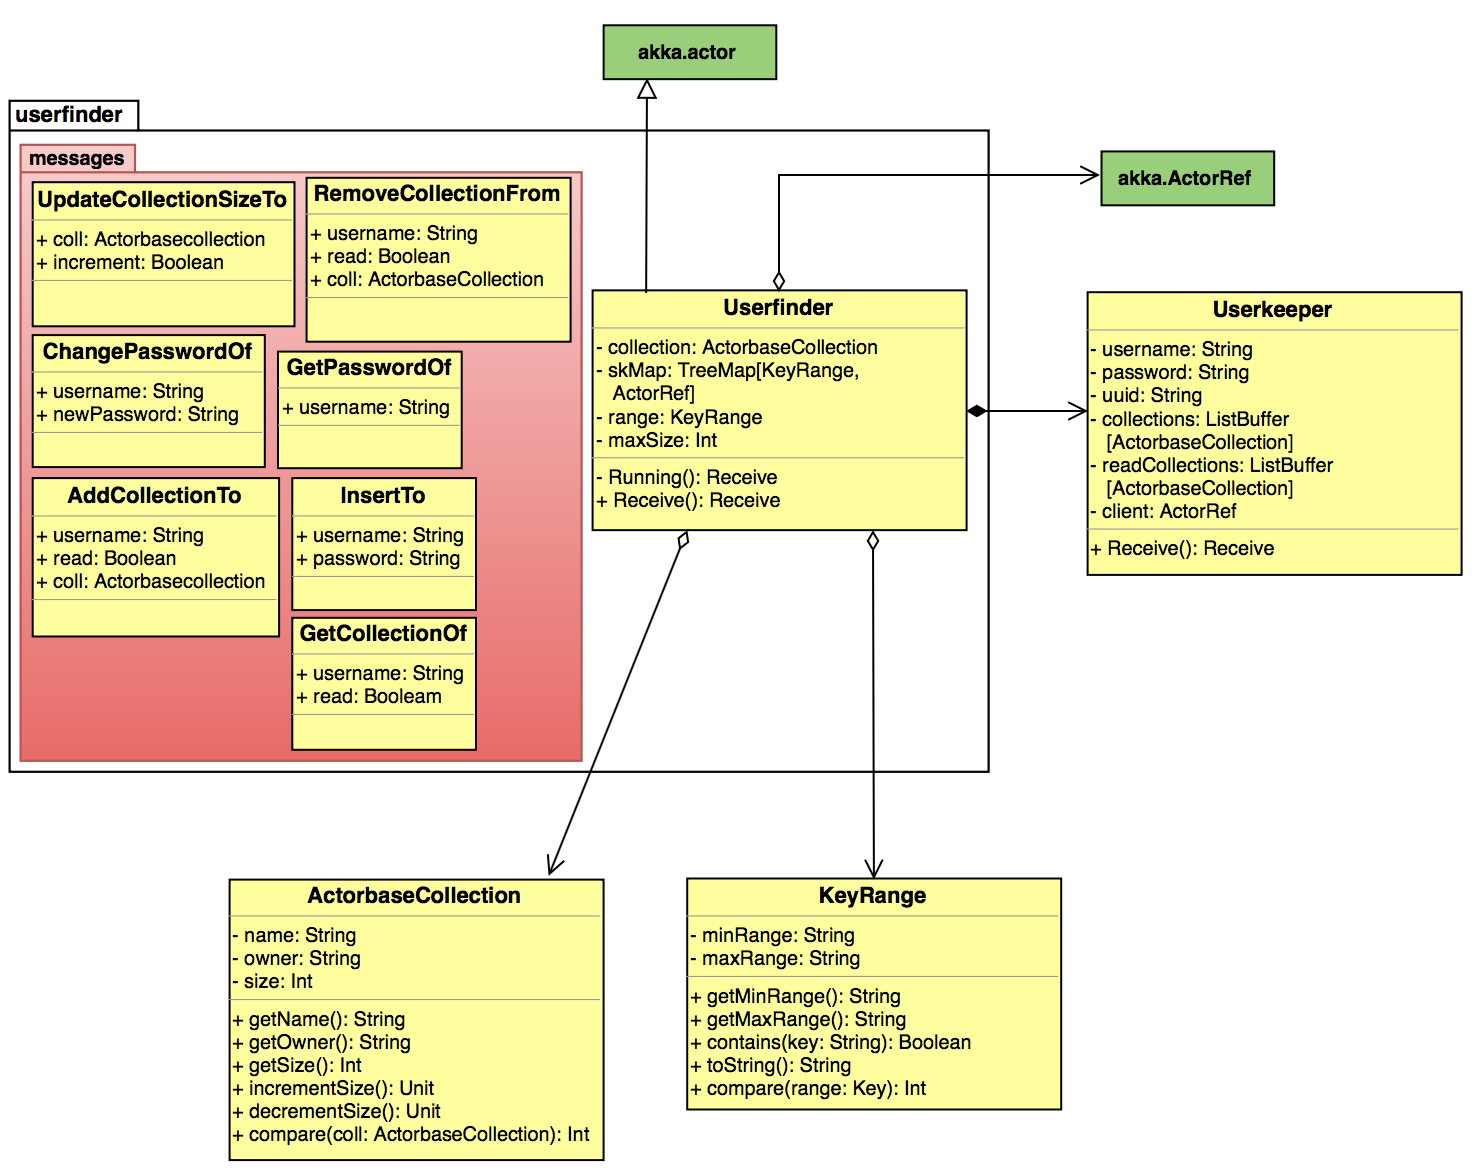
\includegraphics[width=0.8\textwidth,keepaspectratio]{RQ/userfinder.png}
    \caption{Userfinder, visione generale del package}
  \end{center}
\end{figure}

\subsubsection{Descrizione}
Classe che rappresenta un \gloss{attore} di tipo \gloss{Userfinder}.

\subsubsection{Package contenuti}
\begin{itemize}
\item \hyperref[sec:actorbase::actorsystem::userfinder::messages]{actorbase::actorsystem::userfinder::messages}.
\end{itemize}

\subsubsection{Classi}

\paragraph{actorbase::actorsystem::userfinder::Userfinder}
\label{sec:actorbase::actorsystem::userfinder::Userfinder}

\subparagraph{Descrizione}
Classe che rappresenta un \gloss{attore} di tipo \gloss{Userfinder}.

\subparagraph{Utilizzo}
Questa classe viene utilizzata per tener traccia degli attori di tipo
\hyperref[sec:actorbase::actorsystem::userkeeper::Userkeeper]{actorbase::actorsystem::userkeeper::Userkeeper}.

\subparagraph{Classi ereditate}
\begin{itemize}
\item akka::actor::Actor.
\end{itemize}

\subparagraph{Attributi}
\begin{tabular}{| p{3cm} | p{1.5cm} | p{2cm} | p{2cm} | p{8.5cm} |}
  \hline
  Nome & Accesso & Mutabilità & Tipo & Descrizione\\
  \hline
  ukMap & private & immutabile & TreeMap [String, ActorRef] & Rappresenta una mappa contenente come chiavi gli username degli utenti e come valori i riferimenti degli userkeeper che li rappresentano \\
  \hline
\end{tabular}

\subparagraph{Metodi}

\begin{tabular}{| l | l | l | l |}
  \hline
  Nome & Accesso & Tipo di ritorno & Descrizione\\
  \hline
  receive & public &  & Effettua operazioni diverse a seconda del tipo di messaggio ricevuto\\
  \hline
\end{tabular}

\subsection{actorbase::actorsystem::userfinder::messages}
\label{sec:actorbase::actorsystem::userfinder::messages}

\subsubsection{Descrizione}
\gloss{Package} che contiene tutti i messaggi che possono essere ricevuti da
\hyperref[sec:actorbase::actorsystem::userfinder::Userfinder]{actorbase::actorsystem::userfinder::Userfinder}.

\subsubsection{Classi}

\paragraph{actorbase::actorsystem::userfinder::messages::GetPasswordOf}
\label{sec:actorbase::actorsystem::userfinder::messages::GetPasswordOf}

\subparagraph{Descrizione}
Messaggio che indica la richiesta di autenticazione da parte di un utente.\\

\subparagraph{Utilizzo}
Quando l'attore riceve questo messaggio provvederà a inoltrare la richiesta
allo \hyperref[sec:actorbase::actorsystem::userkeeper::Userkeeper]{Userkeeper}
relativo allo username ricevuto.

\subparagraph{Attributi}
\begin{tabular}{| p{3cm} | p{1.5cm} | p{2cm} | p{2cm} | p{8.5cm} |}
  \hline
  Nome & Accesso & Mutabilità & Tipo & Descrizione\\
  \hline
  username & public & immutabile & String & stringa che rappresenta lo username dell'utente che richiede di autenticarsi\\
  \hline
\end{tabular}

\paragraph{actorbase::actorsystem::userfinder::messages::InsertTo}
\label{sec:actorbase::actorsystem::userfinder::messages::InsertTo}

\subparagraph{Descrizione}
Messaggio che indica la richiesta di un aggiunta di un utente nel sistema,
corrisponde con la creazione di un attore \hyperref[sec:actorbase::actorsystem::userkeeper::Userkeeper]{actorbase::\allowbreak{}actorsystem::\allowbreak{}userkeeper::\allowbreak{}Userkeeper}.

\subparagraph{Utilizzo}
Quando l'attore riceve questo messaggio provvederà a creare un attore di tipo \hyperref[sec:actorbase::actorsystem::userkeeper::Userkeeper]{actorbase::\allowbreak{}actorsystem::\allowbreak{}userkeeper::\allowbreak{}Userkeeper}
e l'inserimento del suo riferimento nella propria struttura dati.

\subparagraph{Attributi}
\begin{tabular}{| p{3cm} | p{1.5cm} | p{2cm} | p{2cm} | p{8.5cm} |}
  \hline
  Nome & Accesso & Mutabilità & Tipo & Descrizione\\
  \hline
  username & public & immutabile & String & stringa che rappresenta lo username dell'utente da inserire \\
  \hline
  password & public & immutabile & String & stringa che rappresenta la password dell'utente da inserire \\
  \hline
\end{tabular}

\paragraph{actorbase::actorsystem::userfinder::messages::GetCollectionOf}
\label{sec:actorbase::actorsystem::userfinder::messages::GetCollectionOf}

\subparagraph{Descrizione}
Messaggio che indica la necessità di tornare le collezioni con il tipo di permessi immesso di un utente.

\subparagraph{Utilizzo}
Quando l'attore riceve questo messaggio provvederà a inoltrare la richiesta all'attore di tipo \hyperref[sec:actorbase::actorsystem::userkeeper::Userkeeper]{actorbase::\allowbreak{}actorsystem::\allowbreak{}userkeeper::\allowbreak{}Userkeeper}
che rappresenta l'utente richiesto dal parametro di ingresso.

\subparagraph{Attributi}
\begin{tabular}{| p{3cm} | p{1.5cm} | p{2cm} | p{2cm} | p{8.5cm} |}
  \hline
  Nome & Accesso & Mutabilità & Tipo & Descrizione\\
  \hline
  username & public & immutabile & String & stringa che rappresenta lo username dell'utente cui si vogliono ritornare le collezioni \\
  \hline
  write & public & immutabile & Boolean & Flag che indica se il metodo deve tornare le collezioni su cui l'utente ha permessi in sola lettura (write \= 0) o le collezioni su cui l'utente ha permessi di lettura e scrittura (write \= 1) \\
  \hline
\end{tabular}

\paragraph{actorbase::actorsystem::userfinder::messages::ChangePasswordOf}
\label{sec:actorbase::actorsystem::userfinder::messages::ChangePasswordOf}

\subparagraph{Descrizione}
Messaggio che indica la richiesta di una modifica password di un utente.

\subparagraph{Utilizzo}
Quando l'attore riceve questo messaggio provvederà a inoltrare la richiesta di cambio password all'attore di tipo \hyperref[sec:actorbase::actorsystem::userkeeper::Userkeeper]{actorbase::\allowbreak{}actorsystem::\allowbreak{}userkeeper::\allowbreak{}Userkeeper}
corrispondente all'utente corretto.

\subparagraph{Attributi}
\begin{tabular}{| p{3cm} | p{1.5cm} | p{2cm} | p{2cm} | p{8.5cm} |}
  \hline
  Nome & Accesso & Mutabilità & Tipo & Descrizione\\
  \hline
  username & public & immutabile & String & stringa che rappresenta lo username dell'utente che ha richiesto la modifica password \\
  \hline
  newPassword & public & immutabile & String & stringa che rappresenta la password nuoca dell'utente \\
  \hline
\end{tabular}

\paragraph{actorbase::actorsystem::userfinder::messages::RemoveCollectionFrom}
\label{sec:actorbase::actorsystem::userfinder::messages::RemoveCollectionFrom}

\subparagraph{Descrizione}
Messaggio che indica la richiesta di rimozione di una collezione dalla struttura dati dello \hyperref[sec:actorbase::actorsystem::userkeeper::Userkeeper]{actorbase::\allowbreak{}actorsystem::\allowbreak{}userkeeper::\allowbreak{}Userkeeper} corrispondente.

\subparagraph{Utilizzo}
Quando l'attore riceve questo messaggio provvederà a inoltrare la richiesta
all'attore di tipo \hyperref[sec:actorbase::actorsystem::userkeeper::Userkeeper]{actorbase::\allowbreak{}actorsystem::\allowbreak{}userkeeper::\allowbreak{}Userkeeper}
corrispondente all'utente corretto.

\subparagraph{Attributi}
\begin{tabular}{| p{3cm} | p{1.5cm} | p{2cm} | p{2cm} | p{8.5cm} |}
  \hline
  Nome & Accesso & Mutabilità & Tipo & Descrizione\\
  \hline
  username & public & immutabile & String & stringa che rappresenta lo username dell'utente su cui effettuare l'operazione \\
  \hline
  write & public & immutable & Boolean & flag che rappresenta i permessi che l'utente ha sulla collezione da rimuovere \\
  \hline
  collection & public & immutabile & String & stringa che rappresenta la collezione da rimuovere \\
  \hline
\end{tabular}

\paragraph{actorbase::actorsystem::userfinder::messages::AddCollectionTo}
\label{sec:actorbase::actorsystem::userfinder::messages::AddCollectionTo}

\subparagraph{Descrizione}
Messaggio che indica la richiesta di un aggiunta di una collezione con i permessi inseriti ad un utente nel sistema.

\subparagraph{Utilizzo}
Quando l'attore riceve questo messaggio provvederà a inoltrare la richiesta all'attore di tipo \hyperref[sec:actorbase::actorsystem::userkeeper::Userkeeper]{actorbase::\allowbreak{}actorsystem::\allowbreak{}userkeeper::\allowbreak{}Userkeeper}
corrispondente all'utente su cui effettuare l'operazione.

\subparagraph{Attributi}
\begin{tabular}{| p{3cm} | p{1.5cm} | p{2cm} | p{2cm} | p{8.5cm} |}
  \hline
  Nome & Accesso & Mutabilità & Tipo & Descrizione\\
  \hline
  username & public & immutabile & String & stringa che rappresenta lo username dell'utente a cui aggiungere la collezione \\
  \hline
  write & public & immutable & Boolean & flag che rappresenta i permessi che l'utente ha sulla collezione da aggiungere \\
  \hline
  collection & public & immutabile & String & stringa che rappresenta la collezione da aggiungere \\
  \hline
\end{tabular}

\paragraph{actorbase::actorsystem::userfinder::messages::UpdateCollectionSizeTo}
\label{sec:actorbase::actorsystem::userfinder::messages::UpdateCollectionSizeTo}

\subparagraph{Descrizione}

Messaggio che indica la ncessità di aggiornare il numero di item di una collezione.

\subparagraph{Utilizzo}

Quando \hyperref[sec:actorbase::actorsystem::userfinder::Userfinder]{actorbase::\allowbreak{}actorsystem::\allowbreak{}userfinder::\allowbreak{}Userfinder}
riceve questo messaggio provvederà ad inoltrare all'attore di tipo
\hyperref[sec:actorbase::actorsystem::userkeeper::Userkeeper]{actorbase::\allowbreak{}actorsystem::\allowbreak{}userkeeper::\allowbreak{}Userkeeper}.

\subparagraph{Attributi}
\begin{tabular}{| p{3cm} | p{1.5cm} | p{2cm} | p{2cm} | p{8.5cm} |}
  \hline
  Nome & Accesso & Mutabilità & Tipo & Descrizione\\
  \hline
  collection & public & immutabile & ActorbaseCollection & Collezione di cui aggiornare il contatore \\
  \hline
  increment & public & immutabile & Boolean & Se true causa un incremento del contatore, se false causa un decremento del contatore \\
  \hline
\end{tabular}


%%%%%%%%%%%%%%%%%%%%%%%%%%%%%%%%%%%%%%%%%%%%%%%%%%%%%%%%%%%%%%%%%%%%%%%%
%%%%%%%%%%%%%%%%%%%%%%%%%%%%%%%%%%%%%%%%%%%%%%%%%%%%%%%%%%%%%%%%%%%%%%%%
%%%%%%%%%%%%%%%%%%%%%%%%%%%%%%%%%%%%%%%%%%%%%%%%%%%%%%%%%%%%%%%%%%%%%%%%

\subsection{actorbase::actorsystem::userkeeper} %TODO fatto, non so se ci sia da aggiornare qualcosa, tipo l'immagine, boh
\label{sec:actorbase::actorsystem::userkeeper}

\begin{figure}[H]
  \begin{center}
    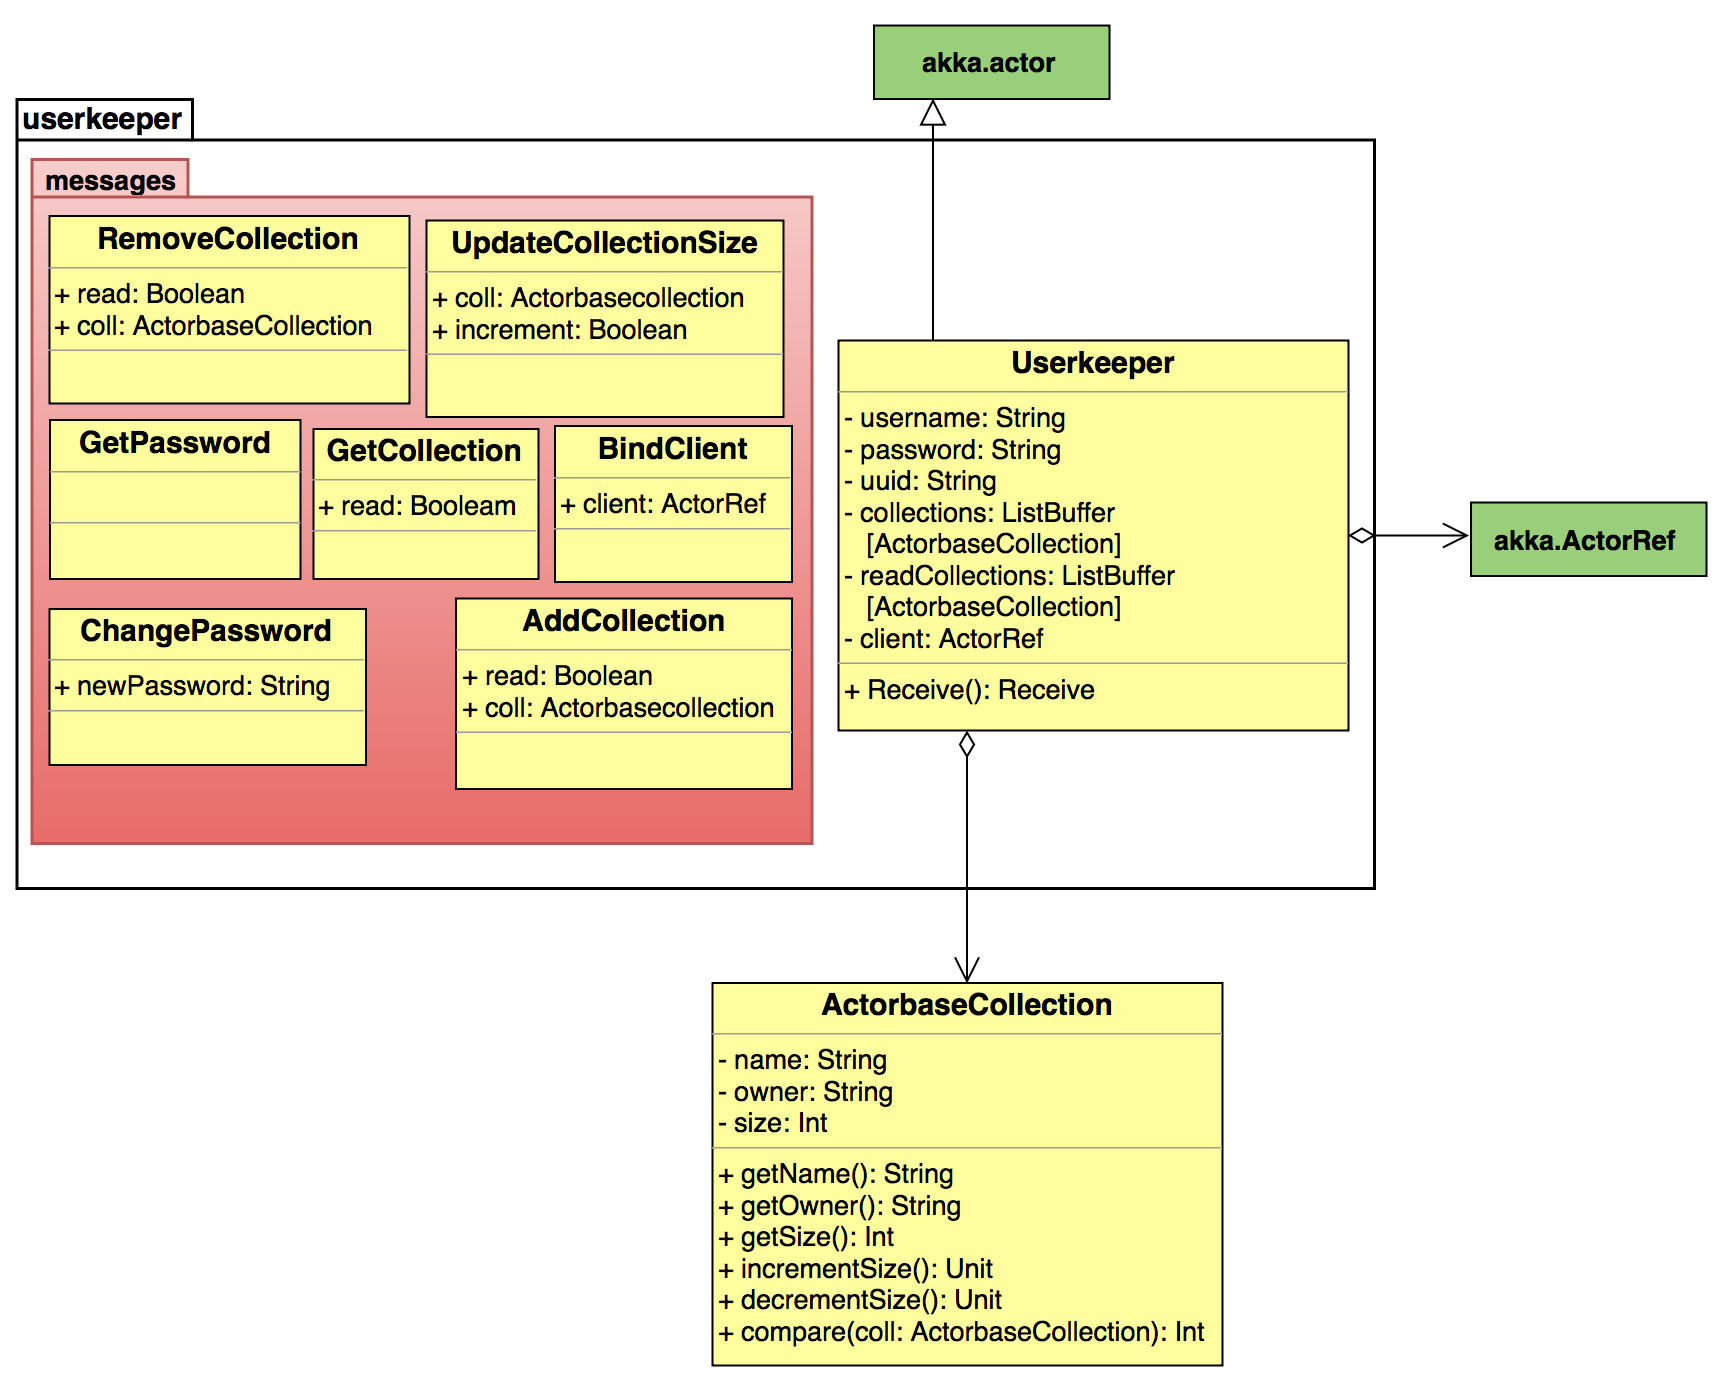
\includegraphics[width=0.8\textwidth,keepaspectratio]{RQ/userkeeper.png}
    \caption{Userkeeper, visione generale del package}
  \end{center}
\end{figure}

\subsubsection{Descrizione}
Classe che rappresenta un \gloss{attore} di tipo \gloss{Userkeeper}.

\subsubsection{Package contenuti}
\begin{itemize}
\item \hyperref[sec:actorbase::actorsystem::userkeeper::messages]{actorbase::actorsystem::userkeeper::messages}.
\end{itemize}

\subsubsection{Classi}

\paragraph{actorbase::actorsystem::userkeeper::Userkeeper}
\label{sec:actorbase::actorsystem::userkeeper::Userkeeper}

\subparagraph{Descrizione}
Classe che rappresenta un \gloss{attore} di tipo \gloss{Userkeeper}.

\subparagraph{Utilizzo}
Questa classe viene utilizzata per salvare gli utenti e i loro dati nel \gloss{database}.

\subparagraph{Classi ereditate}
\begin{itemize}
\item akka::actor::Actor.
\end{itemize}

\subparagraph{Attributi}
\begin{tabular}{| p{3cm} | p{1.5cm} | p{2cm} | p{2cm} | p{8.5cm} |}
  \hline
  Nome & Accesso & Mutabilità & Tipo & Descrizione\\
  \hline
  collections & private & mutabile & ListBuffer [String] & Rappresenta la lista di collezioni di cui l'utente ha permessi di lettura e scrittura \\
  \hline
  readCollections & private & mutabile & ListBuffer [String] & Rappresenta la lista di collezioni di cui l'utente ha permessi di sola lettura \\
  \hline
  client & private & mutabile & ActorRef & Riferimento all'attore di tipo \gloss{ClientActor}. Questo servirà a velocizzare l'aggiornamento del \gloss{ClientActor} \\
  \hline
  username & private & mutabile & String & Stringa che rappresenta l'username dell'utente associato a questo Userkeeper \\
  \hline
  password & private & mutabile & String & Stringa che rappresenta la password dell'utente associato a questo Userkeeper \\
  \hline
  uuid & private & immutable & String & Stringa generata casualmente che rappresenta l'id dell'utente associato a questo Userkeeper \\
  \hline
\end{tabular}

\subparagraph{Metodi}
\begin{tabular}{| l | l | l | l |}
  \hline
  Nome & Accesso & Tipo di ritorno & Descrizione\\
  \hline
  receive & public & Actor.Receive  & Effettua operazioni diverse a seconda del tipo di messaggio ricevuto\\
  \hline
  updateOwnerOfSK & private &  Unit & Metodo che aggiorna il proprietario di tutti gli \hyperref[sec:actorbase::actorsystem::storekeeper::Storekeeper]{Storekeeper} mappati dallo storefinder\\
  \hline
  waitingForRequests & private & Actor.Receive & Metodo che definisce il tipo di messaggio che l'attore \hyperref[sec:actorbase::actorsystem::storefinder::Storefinder]{Storefinder} può ricevere mentre si trova nello stato waitingForRequests\\
  \hline
  processingRequest & private & Actor.Receive & Metodo che definisce il tipo di messaggio che l'attore \hyperref[sec:actorbase::actorsystem::main::storefinder::Storefinder]{Storefinder} può ricevere mentre si trova nello stato processingRequest\\
  \hline
\end{tabular}

\subsection{actorbase::actorsystem::userkeeper::messages}
\label{sec:actorbase::actorsystem::userkeeper::messages}

\subsubsection{Descrizione}

\gloss{Package} che contiene tutti i messaggi che possono essere ricevuti da
\hyperref[sec:actorbase::actorsystem::userkeeper::Userkeeper]{actorbase::actorsystem::userkeeper::Userkeeper}.

\subsubsection{Classi}

\paragraph{actorbase::actorsystem::userkeeper::messages::GetCollections}
\label{sec:actorbase::actorsystem::userkeeper::messages::GetCollections}

\subparagraph{Descrizione}
Messaggio che indica la richiesta della lista di \gloss{collezioni} di cui
l'utente ha permessi in lettura e scrittura.

\subparagraph{Utilizzo}
Quando \hyperref[sec:actorbase::actorsystem::userkeeper::Userkeeper]{actorbase::\allowbreak{}actorsystem::\allowbreak{}userkeeper::\allowbreak{}Userkeeper}
riceve questo messaggio provvederà a restituire all'\gloss{attore} di tipo
\hyperref[sec:actorbase::actorsystem::clientactor::ClientActor]{actorbase::\allowbreak{}actorsystem::\allowbreak{}clientactor::\allowbreak{}ClientActor}
la lista di \gloss{collezioni} di cui l'utente ha permessi in lettura
e scrittura.

\subparagraph{Attributi}
\begin{tabular}{| p{3cm} | p{1.5cm} | p{2cm} | p{2cm} | p{8.5cm} |}
  \hline
  Nome & Accesso & Mutabilità & Tipo & Descrizione\\
  \hline
  write & public & immutabile & Boolean & Booleano che serve a scegliere se il metodo deve tornare la lista di collezioni cui l'utente ha permessi in sola lettura (se write = false) o in lettura e scrittura (se write = true) \\
  \hline
\end{tabular}


\paragraph{actorbase::actorsystem::userkeeper::messages::ChangePassword}
\label{sec:actorbase::actorsystem::userkeeper::messages::ChangePassword}

\subparagraph{Descrizione}
Messaggio che indica la richiesta di cambiamento della password.

\subparagraph{Utilizzo}
Quando \hyperref[sec:actorbase::actorsystem::userkeeper::Userkeeper]{actorbase::\allowbreak{}actorsystem::\allowbreak{}userkeeper::\allowbreak{}Userkeeper}
riceve questo messaggio provvederà a modificare la password dell'utente.

\subparagraph{Attributi}
\begin{tabular}{| p{3cm} | p{1.5cm} | p{2cm} | p{2cm} | p{8.5cm} |}
  \hline
  Nome & Accesso & Mutabilità & Tipo & Descrizione\\
  \hline
  newPassword & public & immutabile & String & stringa che rappresenta la nuova password da assegnare all'utente rappresentato \\
  \hline
\end{tabular}


\paragraph{actorbase::actorsystem::userkeeper::messages::GetPassword}
\label{sec:actorbase::actorsystem::userkeeper::messages::GetPassword}

\subparagraph{Descrizione}

Messaggio che indica la richiesta della password.

\subparagraph{Utilizzo}

Quando \hyperref[sec:actorbase::actorsystem::userkeeper::Userkeeper]{actorbase::\allowbreak{}actorsystem::\allowbreak{}userkeeper::\allowbreak{}Userkeeper}
riceve questo messaggio provvederà a inviare la password all'\gloss{attore} di tipo
\hyperref[sec:actorbase::actorsystem::clientactor::ClientActor]{actorbase::\allowbreak{}actorsystem::\allowbreak{}clientactor::\allowbreak{}ClientActor}.

\paragraph{actorbase::actorsystem::userkeeper::messages::RemoveCollection}
\label{sec:actorbase::actorsystem::userkeeper::messages::RemoveCollection}

\subparagraph{Descrizione}

Messaggio che indica la richiesta di rimozione di una \gloss{collezione} dalla
lista contenente le \gloss{collezioni} di cui l'utente ha permessi in lettura
o in scrittura.

\subparagraph{Utilizzo}

Quando \hyperref[sec:actorbase::actorsystem::userkeeper::Userkeeper]{actorbase::\allowbreak{}actorsystem::\allowbreak{}userkeeper::\allowbreak{}Userkeeper}
riceve questo messaggio provvederà a rimuovere la \gloss{collezione} desiderata
dalla lista contenente le \gloss{collezioni} di cui l'utente ha permessi in
lettura o in scrittura.

\subparagraph{Attributi}
\begin{tabular}{| p{3cm} | p{1.5cm} | p{2cm} | p{2cm} | p{8.5cm} |}
  \hline
  Nome & Accesso & Mutabilità & Tipo & Descrizione\\
  \hline
  write & public & immutabile & Boolean & Boolean che rappresenta i permessi dell'utente sulla collezione da rimuovere ( \=0 se sola lettura e \=1 se lettura e scrittura) \\
  \hline
  collection & public & immutabile & String & Stringa che rappresenta il nome della collezione da rimuovere \\
  \hline
\end{tabular}


\paragraph{actorbase::actorsystem::userkeeper::messages::AddCollection}
\label{sec:actorbase::actorsystem::userkeeper::messages::AddCollection}

\subparagraph{Descrizione}

Messaggio che indica la richiesta di aggiunta di una \gloss{collezione} dalla
lista contenente le \gloss{collezioni} di cui l'utente ha permessi in lettura
o in lettura e scrittura.

\subparagraph{Utilizzo}

Quando \hyperref[sec:actorbase::actorsystem::userkeeper::Userkeeper]{actorbase::\allowbreak{}actorsystem::\allowbreak{}userkeeper::\allowbreak{}Userkeeper}
riceve questo messaggio provvederà ad aggiungere la \gloss{collezione} desiderata
dalla lista contenente le \gloss{collezioni} di cui l'utente ha permessi in
lettura o in lettura e scrittura.

\subparagraph{Attributi}
\begin{tabular}{| p{3cm} | p{1.5cm} | p{2cm} | p{2cm} | p{8.5cm} |}
  \hline
  Nome & Accesso & Mutabilità & Tipo & Descrizione \\
  \hline
  write & public & immutabile & Boolean & Boolean che rappresenta i permessi dell'utente sulla collezione da aggiungere ( \=0 se sola lettura e \=1 se lettura e scrittura) \\
  \hline
  collection & public & immutabile & String & Stringa che rappresenta il nome della collezione da aggiungere \\
  \hline
\end{tabular}


\paragraph{actorbase::actorsystem::userkeeper::messages::BindClient}
\label{sec:actorbase::actorsystem::userkeeper::messages::BindClient}

\subparagraph{Descrizione}

Messaggio che indica la richiesta di collegamento con un \gloss{ClientActor}.

\subparagraph{Utilizzo}

Quando \hyperref[sec:actorbase::actorsystem::userkeeper::Userkeeper]{actorbase::\allowbreak{}actorsystem::\allowbreak{}userkeeper::\allowbreak{}Userkeeper}
riceve questo messaggio provvederà a salvarsi il riferimento dell'\gloss{attore} di tipo
\hyperref[sec:actorbase::actorsystem::clientactor::ClientActor]{actorbase::\allowbreak{}actorsystem::\allowbreak{}clientactor::\allowbreak{}ClientActor}
che ha inviato questo messaggio.

\subparagraph{Attributi}
\begin{tabular}{| p{3cm} | p{1.5cm} | p{2cm} | p{2cm} | p{8.5cm} |}
  \hline
  Nome & Accesso & Mutabilità & Tipo & Descrizione\\
  \hline
  client & public & immutabile & ActorRef & Riferimento all'attore del tipo \gloss{ClientActor} che si occupa delle richieste dell'utente rappresentato da questo Userkeeper \\
  \hline
\end{tabular}

\paragraph{actorbase::actorsystem::userkeeper::messages::UpdateCollectionSize}
\label{sec:actorbase::actorsystem::userkeeper::messages::UpdateCollectionSize}

\subparagraph{Descrizione}

Messaggio che aggiorna il numero di item di una collezione.

\subparagraph{Utilizzo}

Quando \hyperref[sec:actorbase::actorsystem::userkeeper::Userkeeper]{actorbase::\allowbreak{}actorsystem::\allowbreak{}userkeeper::\allowbreak{}Userkeeper}
riceve questo messaggio provvederà ad aggiornare il contatore relativo al numero di oggetti
nella collezione.

\subparagraph{Attributi}
\begin{tabular}{| p{3cm} | p{1.5cm} | p{2cm} | p{2cm} | p{8.5cm} |}
  \hline
  Nome & Accesso & Mutabilità & Tipo & Descrizione\\
  \hline
  collection & public & immutabile & ActorbaseCollection & Collezione di cui aggiornare il contatore \\
  \hline
  increment & public & immutabile & Boolean & Se true causa un incremento del contatore, se false causa un decremento del contatore \\
  \hline
\end{tabular}

%%%%%%%%%%%%%%%%%%%%%%%%%%%%%%%%%%%%%%%%%%%%%%%%%%%%%%%%%%%%%%%%%%%%%%%%
%%%%%%%%%%%%%%%%%%%%%%%%%%%%%%%%%%%%%%%%%%%%%%%%%%%%%%%%%%%%%%%%%%%%%%%%
%%%%%%%%%%%%%%%%%%%%%%%%%%%%%%%%%%%%%%%%%%%%%%%%%%%%%%%%%%%%%%%%%%%%%%%%

\subsection{actorbase::actorsystem::storefinder} %TODO DA controllare e finire
\label{sec:actorbase::actorsystem::storefinder}

\begin{figure}[H]
  \begin{center}
    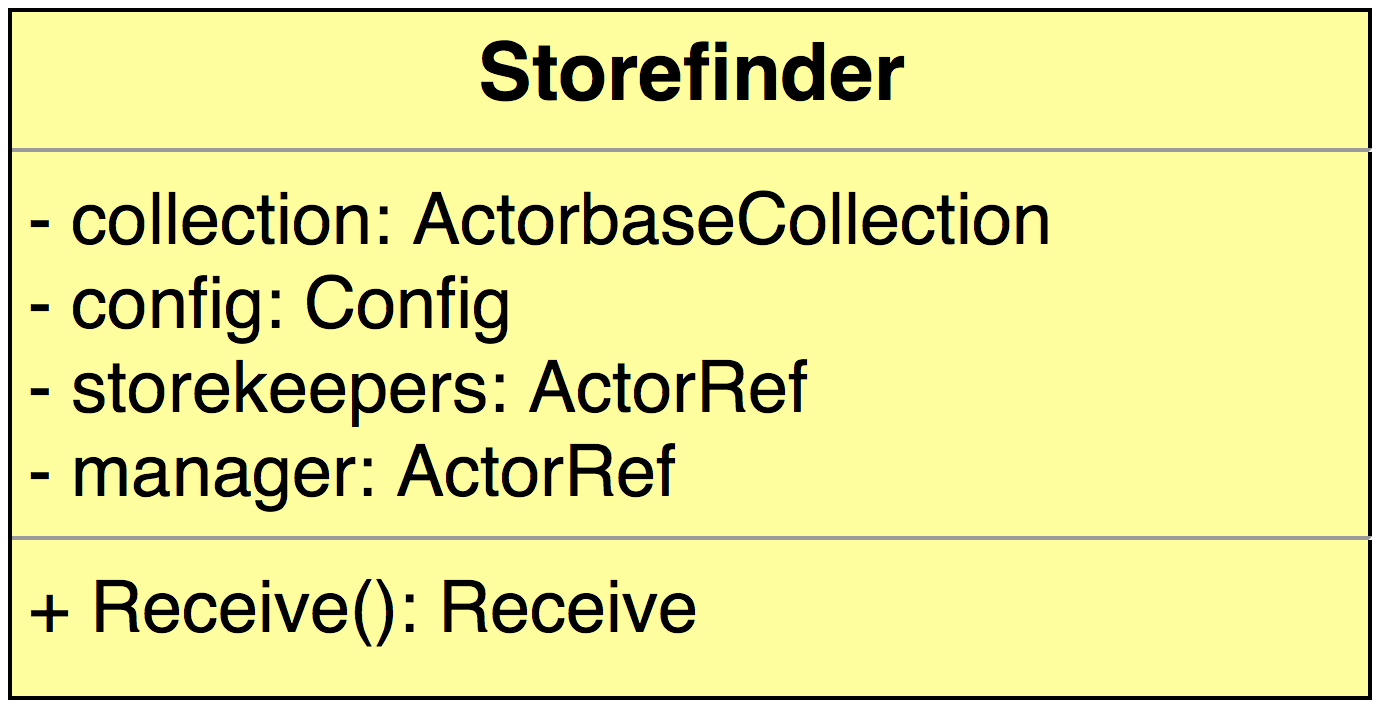
\includegraphics[width=0.8\textwidth,keepaspectratio]{RQ/storefinder.png}
    \caption{Storefinder e interazioni con main}
  \end{center}
\end{figure}

\subsubsection{Descrizione}
Classe che rappresenta un \gloss{attore} di tipo \gloss{Storefinder}.

\subsubsection{Package contenuti}
\begin{itemize}
\item \hyperref[sec:actorbase::actorsystem::storefinder::messages]{actorbase::actorsystem::storefinder::messages}.
\end{itemize}

\subsubsection{Classi}

\paragraph{actorbase::actorsystem::storefinder::Storefinder}
\label{sec:actorbase::actorsystem::storefinder::Storefinder}

\subparagraph{Descrizione}

Classe che rappresenta un \gloss{attore} di tipo \gloss{Storefinder}.

\subparagraph{Utilizzo}
Questa classe viene utilizzata per tener traccia degli attori di tipo
\hyperref[sec:actorbase::actorsystem::storekeeper::Storekeeper]{actorbase::actorsystem::storekeeper::Storekeeper}.

\subparagraph{Classi ereditate}

\begin{itemize}

\item akka::actor::Actor.

\end{itemize}

\subparagraph{Attributi}

\begin{tabular}{| p{3cm} | p{1.5cm} | p{2cm} | p{2cm} | p{8.5cm} |}
  \hline
  Nome & Accesso & Mutabilità & Tipo & Descrizione\\
  \hline
  skMap & private & mutabile & TreeMap [KeyRange, ActorRef] & Rappresenta la mappa di attori di tipo storekeeper relativi alla collezione \\
  \hline
  collection & private & mutabile & actorbaseCollection & Rappresenta il nome della collezione che va a rappresentare\\
  \hline
  range & private & mutabile & KeyRange & Rappresenta l'intervallo delle chiavi mappabili nel particolare storefinder\\
  \hline
  maxSize & private & immutabile & int & Rappresenta la grandezza massima della collezione\\
  \hline
\end{tabular}

\subparagraph{Metodi}

\begin{tabular}{| l | l | l | l |}
  \hline
  Nome & Accesso & Tipo di ritorno & Descrizione\\
  \hline
  receive & public &  & Effettua operazioni diverse a seconda del tipo di messaggio ricevuto\\
  \hline
\end{tabular}

\subsection{actorbase::actorsystem::storefinder::messages}
\label{sec:actorbase::actorsystem::storefinder::messages}

\subsubsection{Descrizione}

\gloss{Package} che contiene tutti i messaggi che possono essere ricevuti da
\hyperref[sec:actorbase::actorsystem::storefinder::Storefinder]{actorbase::actorsystem::storefinder::Storefinder}.

\subsubsection{Classi}

\paragraph{actorbase::actorsystem::storefinder::messages::DuplicationRequestSK}
\label{sec:actorbase::actorsystem::storefinder::messages::DuplicationRequestSK}

\subparagraph{Descrizione}
Messaggio atto ad aggiornare uno Storefinder a seguito di una duplicazione
di un attore di tipo Storekeeper.\\

\subparagraph{Utilizzo}
Quando \hyperref[sec:actorbase::actorsystem::storefinder::Storefinder]{actorbase::\allowbreak{}actorsystem::\allowbreak{}storefinder::\allowbreak{}Storefinder}
riceve questo messaggio provvederà ad aggiornare la sua struttura dati.\\In
particolare aggiornerà i range di chiavi contenuti dagli Storekeeper presenti
nella sua struttura dati.

\subparagraph{Attributi}  % TODO da fare quando il metodo sarà fatto
\begin{tabular}{| p{3cm} | p{1.5cm} | p{2cm} | p{2cm} | p{8.5cm} |}
  \hline
  Nome & Accesso & Mutabilità & Tipo & Descrizione\\
  \hline
  oldKeyRange & public & immutabile & \hyperref[sec:actorbase::actorsystem::utils::KeyRange]{KeyRange} & rappresenta il \hyperref[sec:actorbase::actorsystem::utils::KeyRange]{KeyRange} da duplicare\\
  \hline
  leftRange & public & immutabile & \hyperref[sec:actorbase::actorsystem::utils::KeyRange]{KeyRange} & rappresenta il \hyperref[sec:actorbase::actorsystem::utils::KeyRange]{KeyRange} da assegnare allo \hyperref[sec:actorbase::actorsystem::storekeeper::Storekeeper]{Storekeeper} duplicato \\
  \hline
  map & public & immutable & struttura dati dello \hyperref[sec:actorbase::actorsystem::storekeeper::Storekeeper]{Storekeeper} da creare\\
  \hline
  rightRange & public & immutabile & \hyperref[sec:actorbase::actorsystem::utils::KeyRange]{KeyRange} & rappresenta il \hyperref[sec:actorbase::actorsystem::utils::KeyRange]{KeyRange} da assegnare allo \hyperref[sec:actorbase::actorsystem::storekeeper::Storekeeper]{Storekeeper} da creare\\
  \hline
\end{tabular}


\paragraph{actorbase::actorsystem::storefinder::messages::GetItem}
\label{sec:actorbase::actorsystem::storefinder::messages::GetItem}

\subparagraph{Descrizione}

Messaggio che indica la richiesta di un \gloss{item}.

\subparagraph{Utilizzo}

Quando \hyperref[sec:actorbase::actorsystem::storefinder::Storefinder]{actorbase::\allowbreak{}actorsystem::\allowbreak{}storefinder::\allowbreak{}Storefinder}
riceve questo messaggio provvederà a inoltrare la richiesta all'\gloss{attore} di tipo
\hyperref[sec:actorbase::actorsystem::storekeeper::Storekeeper]{actorbase::\allowbreak{}actorsystem::\allowbreak{}storekeeper::\allowbreak{}Storekeeper}
che contiene l'\gloss{item} cercato.

\subparagraph{Attributi}
\begin{tabular}{| p{3cm} | p{1.5cm} | p{2cm} | p{2cm} | p{8.5cm} |}
  \hline
  Nome & Accesso & Mutabilità & Tipo & Descrizione\\
  \hline
  key & public & immutabile & String & chiave che rappresenta l'\gloss{item} cercato\\
  \hline
\end{tabular}

\paragraph{actorbase::actorsystem::storefinder::messages::RemoveItem}
\label{sec:actorbase::actorsystem::storefinder::messages::RemoveItem}

\subparagraph{Descrizione}

Messaggio che indica la richiesta di rimozione di un \gloss{item}.

\subparagraph{Utilizzo}

Quando \hyperref[sec:actorbase::actorsystem::storefinder::Storefinder]{actorbase::\allowbreak{}actorsystem::\allowbreak{}storefinder::\allowbreak{}Storefinder}
riceve questo messaggio provvederà a inoltrare la richiesta all'\gloss{attore} di tipo
\hyperref[sec:actorbase::actorsystem::storekeeper::Storekeeper]{actorbase::\allowbreak{}actorsystem::\allowbreak{}storekeeper::\allowbreak{}Storekeeper}
che contiene l'\gloss{item} da rimuovere.

\subparagraph{Attributi}
\begin{tabular}{| p{3cm} | p{1.5cm} | p{2cm} | p{2cm} | p{8.5cm} |}
  \hline
  Nome & Accesso & Mutabilità & Tipo & Descrizione\\
  \hline
  key & public & immutabile & String & chiave che rappresenta l'\gloss{item} da rimuovere\\
  \hline
\end{tabular}

\paragraph{actorbase::actorsystem::storefinder::messages::Insert}
\label{sec:actorbase::actorsystem::storefinder::messages::Insert}

\subparagraph{Descrizione}

Messaggio che indica la richiesta di inserimento di un \gloss{item}.

\subparagraph{Utilizzo}

Quando \hyperref[sec:actorbase::actorsystem::storefinder::Storefinder]{actorbase::\allowbreak{}actorsystem::\allowbreak{}storefinder::\allowbreak{}Storefinder}
riceve questo messaggio provvederà a inoltrare la richiesta all'\gloss{attore} di tipo
\hyperref[sec:actorbase::actorsystem::storekeeper::Storekeeper]{actorbase::\allowbreak{}actorsystem::\allowbreak{}storekeeper::\allowbreak{}Storekeeper}
destinato a ricevere l'\gloss{item} da inserire.

\subparagraph{Attributi}
\begin{tabular}{| p{3cm} | p{1.5cm} | p{2cm} | p{2cm} | p{8.5cm} |}
  \hline
  Nome & Accesso & Mutabilità & Tipo & Descrizione\\
  \hline
  key & public & immutabile & String & chiave che rappresenta l'\gloss{item} da inserire\\
  \hline
  value & public & immutable & Any & valore dell'\gloss{item} da inserire\\
  \hline
  update & public & immutable & Boolean & flag che serve a sapere se l'\gloss{item} da inserire può sovrascrivere un \gloss{item} già presente o no\\
  \hline
\end{tabular}

\paragraph{actorbase::actorsystem::storefinder::messages::GetAllItem}
\label{sec:actorbase::actorsystem::storefinder::messages::GetAllItem}

\subparagraph{Descrizione}

Messaggio che indica la richiesta di restituzione di tutti gli
\gloss{item} mappati dallo Storefinder.

\subparagraph{Utilizzo}

Quando \hyperref[sec:actorbase::actorsystem::storefinder::Storefinder]{actorbase::\allowbreak{}actorsystem::\allowbreak{}storefinder::\allowbreak{}Storefinder}
riceve questo messaggio provvederà a inoltrare la richiesta a tutti gli attori
di tipo
\hyperref[sec:actorbase::actorsystem::storekeeper::Storekeeper]{actorbase::\allowbreak{}actorsystem::\allowbreak{}storekeeper::\allowbreak{}Storekeeper}
che dovranno restituire tutti gli \gloss{items} contenuti in essi.

\paragraph{actorbase::actorsystem::storefinder::messages::GetAllItemResponse}
\label{sec:actorbase::actorsystem::storefinder::messages::GetAllItemResponse}

\subparagraph{Descrizione}

Messaggio che serve per comporre l'intera collezione da restituire all'utente

\subparagraph{Utilizzo}

Quando \hyperref[sec:actorbase::actorsystem::storefinder::Storefinder]{Storefinder}
riceve questo messaggio non farà altro che richiamare il metodo
\hyperref[sec:actorbase::actorsystem::main::messages::GetItemFromResponse]{GetItemFromResponse} del Main.

\subparagraph{Attributi}
\begin{tabular}{| p{3cm} | p{1.5cm} | p{2cm} | p{2cm} | p{8.5cm} |}
  \hline
  Nome & Accesso & Mutabilità & Tipo & Descrizione\\
  \hline
  clientRef & public & immutabile & ActorRef & Riferimento del client che richiede la collezione\\
  \hline
  items & public & immutabile & TreeMap[String, Any] & rappresenta un pezzo della collezione richiesta\\
  \hline
\end{tabular}

\paragraph{actorbase::actorsystem::storefinder::messages::UpdateCollectionSize}
\label{sec:actorbase::actorsystem::storefinder::messages::UpdateCollectionSize}

\subparagraph{Descrizione}

Messaggio che incrementa il numero delle coppie chiave-valore alla collezione

\subparagraph{Utilizzo}

Quando \hyperref[sec:actorbase::actorsystem::storefinder::Storefinder]{Storefinder}
riceve questo messaggio non farà altro che richiamare il metodo
\hyperref[sec:actorbase::actorsystem::main::messages::UpdateCollectionSize]{UpdateCollectionSize} del Main.

\subparagraph{Attributi}
\begin{tabular}{| p{3cm} | p{1.5cm} | p{2cm} | p{2cm} | p{8.5cm} |}
  \hline
  Nome & Accesso & Mutabilità & Tipo & Descrizione\\
  \hline
  collection & public & immutable & ActorbaseCollection & Nome della collezione che si vuole incrementare\\
  \hline
  increment & public & immutable & boolean & indica se deve esser fatto un incremento (true) o un decremento (false)\\
  \hline
\end{tabular}

%%%%%%%%%%%%%%%%%%%%%%%%%%%%%%%%%%%%%%%%%%%%%%%%%%%%%%%%%%%%%%%%%%%%%%%%
%%%%%%%%%%%%%%%%%%%%%%%%%%%%%%%%%%%%%%%%%%%%%%%%%%%%%%%%%%%%%%%%%%%%%%%%
%%%%%%%%%%%%%%%%%%%%%%%%%%%%%%%%%%%%%%%%%%%%%%%%%%%%%%%%%%%%%%%%%%%%%%%%

\subsection{actorbase::actorsystem::storekeeper}
\label{sec:actorbase::actorsystem::storekeeper}

\begin{figure}[H]
  \begin{center}
    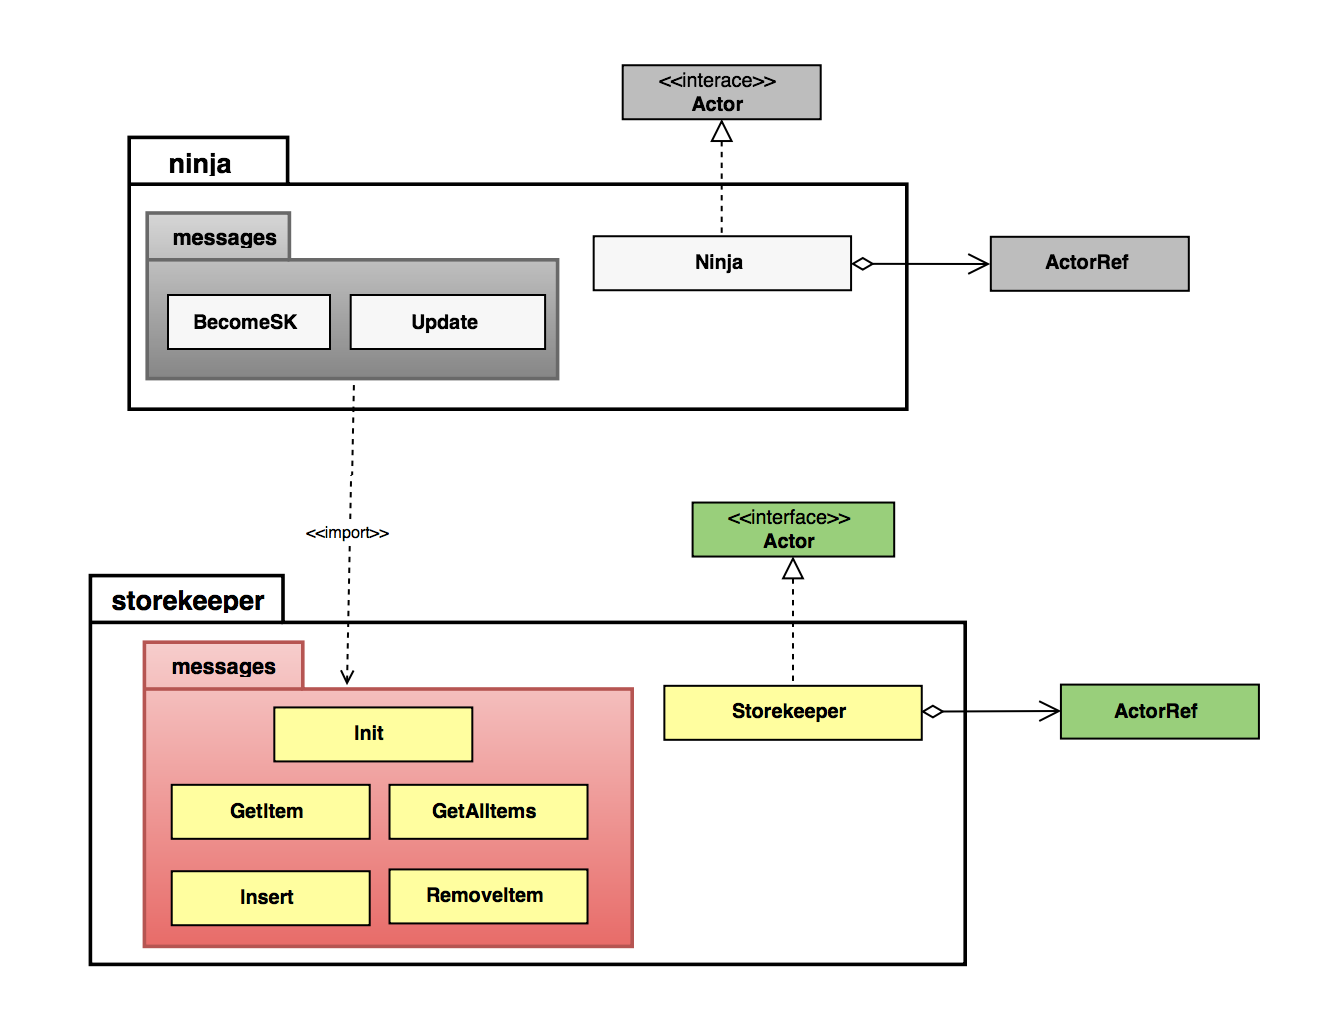
\includegraphics[width=0.8\textwidth,keepaspectratio]{RQ/Storekeeper.png}
    \caption{Storekeeper e interazioni con ninja}
  \end{center}
\end{figure}

\subsubsection{Descrizione}
\gloss{Package} che rappresenta l'\gloss{attore} di tipo \gloss{Storekeeper}.

\subsubsection{Package contenuti}
\begin{itemize}
\item \hyperref[sec:actorbase::actorsystem::storekeeper::messages]{actorbase::actorsystem::storekeeper::messages}.
\end{itemize}

\subsubsection{Classi}

\paragraph{actorbase::actorsystem::storekeeper::Storekeeper}
\label{sec:actorbase::actorsystem::storekeeper::Storekeeper}

\subparagraph{Descrizione}
Classe che rappresenta un \gloss{attore} di tipo \gloss{Storekeeper}.

\subparagraph{Utilizzo}
Questa classe viene utilizzata per salvare nel \gloss{database} gli item.

\subparagraph{Classi ereditate}
\begin{itemize}
\item akka::actor::Actor.
\end{itemize}

\subparagraph{Attributi}

\begin{tabular}{| p{3cm} | p{1.5cm} | p{2cm} | p{2cm} | p{8.5cm} |}
  \hline
  Nome & Accesso & Mutabilità & Tipo & Descrizione\\
  \hline
  parentRef & private & mutabile & ActorRef & Riferimento all'attore di tipo \gloss{Storefinder} che contiene l'attore di tipo \gloss{Storekeeper} \\
  \hline
  data & private & mutabile & TreeMap [String, Any] & Rappresenta l'insieme di \gloss{item} contenuta nell'attore\\
  \hline
  range & private & mutabile & KeyRange & Rappresenta il range di chiavi contenuta nell'attore\\
  \hline
  collection & private & immutabile & ActorbaseCollection & Rappresenta la collezione a cui lo \gloss{Storekeeper} appartiene\\
  \hline
  parentRange & private & mutabile & KeyRange & Rappresenta il range di chiavi contenuta nell'attore di tipo \gloss{Storefinder} che contiene lo \gloss{Storekeeper}\\
  \hline
  maxSize & private & immutabile & Int & Rappresenta il numero massimo di \gloss{item} che possono essere contenuti\\
  \hline
  warehouseman & private & immutabile & ActorRef & Rappresenta il \gloss{Warehouseman} responsabile del salvataggio dei dati dello \gloss{Storekeeper}\\
  \hline
\end{tabular}

\subparagraph{Metodi}

\begin{tabular}{| l | l | l | l |}
  \hline
  Nome & Accesso & Tipo di ritorno & Descrizione\\
  \hline
  receive & public &  & Effettua operazioni diverse a seconda del tipo di messaggio ricevuto\\
  \hline
  insertOrUpdate & private & & Inserisce un item nella collezione\\
  \hline
\end{tabular}

\subparagraph{Parametri}

\begin{center}
  \textbf{insertOrUpdate}\\
\end{center}
\begin{tabular}{| l | l | l |}
  \hline
  Nome & Tipo & Descrizione\\
  \hline
  update & Boolean & Variabile che, se uguale a true, indica che l'inserimento da effettuare è con sovrascrittura\\
  \hline
  key & String & Variabile che indica la chiave dell'\gloss{item} da inserire\\
  \hline
  value & Any & Variabile che indica il valore dell'\gloss{item} da inserire\\
  \hline
\end{tabular}

\subsection{actorbase::actorsystem::storekeeper::messages}
\label{sec:actorbase::actorsystem::storekeeper::messages}

\subsubsection{Descrizione}

\gloss{Package} che contiene tutti i messaggi che possono essere
ricevuti dall'\gloss{attore} di tipo
\hyperref[sec:actorbase::actorsystem::storekeeper::Storekeeper]{actorbase::\allowbreak{}actorsystem::\allowbreak{}storekeeper::\allowbreak{}Storekeeper}.

\subsubsection{Classi}

\paragraph{actorbase::actorsystem::storekeeper::messages::GetItem}
\label{sec:actorbase::actorsystem::storekeeper::messages::GetItem}

\subparagraph{Descrizione}

Messaggio che richiede un \gloss{item} contenuto dall'\gloss{attore}
\gloss{Storekeeper} che lo riceve.

\subparagraph{Utilizzo}

Quando \hyperref[sec:actorbase::actorsystem::storekeeper::Storekeeper]{actorbase::actorsystem::storekeeper::Storekeeper}
riceve questo messaggio risponde mandando l'\gloss{item} cercato all'\gloss{attore} di tipo
\hyperref[sec:actorbase::actorsystem::clientactor::ClientActor]{actorbase::actorsystem::clientactor::ClientActor}
che aveva effettuato la richiesta.

\subparagraph{Attributi}
\begin{tabular}{| p{3cm} | p{1.5cm} | p{2cm} | p{2cm} | p{8.5cm} |}
  \hline
  Nome & Accesso & Mutabilità & Tipo & Descrizione\\
  \hline
  key & public & immutabile & String & chiave che rappresenta l'\gloss{item} cercato\\
  \hline
\end{tabular}

\paragraph{actorbase::actorsystem::storekeeper::messages::GetAllItem}
\label{sec:actorbase::actorsystem::storekeeper::messages::GetAllItem}

\subparagraph{Descrizione}

Messaggio che richiede gli \gloss{item} contenuti dall'\gloss{attore}
\gloss{Storekeeper} che lo riceve.

\subparagraph{Utilizzo}

Quando \hyperref[sec:actorbase::actorsystem::storekeeper::Storekeeper]{actorbase::actorsystem::storekeeper::Storekeeper}
riceve questo messaggio risponde mandando gli \gloss{item} all'\gloss{attore} di tipo
\hyperref[sec:actorbase::actorsystem::clientactor::ClientActor]{actorbase::actorsystem::clientactor::ClientActor}
che aveva effettuato la richiesta.

\paragraph{actorbase::actorsystem::storekeeper::messages::Insert}
\label{sec:actorbase::actorsystem::storekeeper::messages::Insert}

\subparagraph{Descrizione}

Messaggio che richiede l'inserimento di un \gloss{item}.

\subparagraph{Utilizzo}

Quando \hyperref[sec:actorbase::actorsystem::storekeeper::Storekeeper]{actorbase::actorsystem::storekeeper::Storekeeper}
riceve questo messaggio inserisce l'\gloss{item} nel suo attributo data.

\subparagraph{Attributi}
\begin{tabular}{| p{3cm} | p{1.5cm} | p{2cm} | p{2cm} | p{8.5cm} |}
  \hline
  Nome & Accesso & Mutabilità & Tipo & Descrizione\\
  \hline
  key & public & immutabile & String & Chiave che rappresenta l'\gloss{item} da inserire\\
  \hline
  value & public & immutabile & Any & Valore dell'\gloss{item} da inserire\\
  \hline
  update & public & immutabile & Boolean & Indica se l'inserimento da effettuare sia con o senza sovrascrittura\\
  \hline
\end{tabular}

\paragraph{actorbase::actorsystem::storekeeper::messages::RemoveItem}
\label{sec:actorbase::actorsystem::storekeeper::messages::RemoveItem}

\subparagraph{Descrizione}

Messaggio che richiede la rimozione di un \gloss{item}.

\subparagraph{Utilizzo}

Quando \hyperref[sec:actorbase::actorsystem::storekeeper::Storekeeper]{actorbase::actorsystem::storekeeper::Storekeeper}
riceve questo messaggio rimuove l'\gloss{item}.

\subparagraph{Attributi}
\begin{tabular}{| p{3cm} | p{1.5cm} | p{2cm} | p{2cm} | p{8.5cm} |}
  \hline
  Nome & Accesso & Mutabilità & Tipo & Descrizione\\
  \hline
  key & public & immutabile & String & Chiave che rappresenta l'\gloss{item} da rimuovere\\
  \hline
\end{tabular}

\paragraph{actorbase::actorsystem::storekeeper::messages::UpdateOwnerOfSk}
\label{sec:actorbase::actorsystem::storekeeper::messages::UpdateOwnerOfSk}

\subparagraph{Descrizione}

Messaggio che richiede l'update del campo dati che rappresenta lo \hyperref[sec:actorbase::actorsystem::storefinder::Storefinder]{Storefinder} che contiene lo \hyperref[sec:actorbase::actorsystem::storekeeper::Storekeeper]{Storekeeper} che ha ricevuto il messaggio.

\subparagraph{Utilizzo}

Quando \hyperref[sec:actorbase::actorsystem::storekeeper::Storekeeper]{Storekeeper}
riceve questo messaggio aggiorna il campo dati relativo allo \hyperref[sec:actorbase::actorsystem::storefinder::Storefinder]{Storefinder} che lo contiene.

\subparagraph{Attributi}
\begin{tabular}{| p{3cm} | p{1.5cm} | p{2cm} | p{2cm} | p{8.5cm} |}
  \hline
  Nome & Accesso & Mutabilità & Tipo & Descrizione\\
  \hline
  newParent & public & immutabile & ActorRef & Rappresenta lo \hyperref[sec:actorbase::actorsystem::storefinder::Storefinder]{Storefinder} che diventerà padre \\
  \hline
  newRange & public & immutabile & KeyRange & Rappresenta il range dello \hyperref[sec:actorbase::actorsystem::storefinder::Storefinder]{Storefinder} che diventerà padre \\
  \hline
\end{tabular}

\paragraph{actorbase::actorsystem::storekeeper::messages::Update}
\label{sec:actorbase::actorsystem::storekeeper::messages::Update}

\subparagraph{Descrizione}

Messaggio che richiede l'update dell'\gloss{attore} che lo riceve.

\subparagraph{Utilizzo}

Quando \hyperref[sec:actorbase::actorsystem::storekeeper::Storekeeper]{actorbase::actorsystem::storekeeper::Storekeeper}
riceve questo messaggio aggiorna gli \gloss{item} che contiene.

\paragraph{actorbase::actorsystem::storekeeper::messages::BecomeSK}
\label{sec:actorbase::actorsystem::storekeeper::messages::BecomeSK}

\subparagraph{Descrizione}

Messaggio che richiede che l'\gloss{attore} di tipo \gloss{Ninja} diventi di tipo
\gloss{Storekeeper}.

\subparagraph{Utilizzo}
Quando \hyperref[sec:actorbase::actorsystem::storekeeper::Storekeeper]{actorbase::actorsystem::storekeeper::Storekeeper}
riceve questo messaggio ed è attualmente un attore di tipo \gloss{Ninja},
esso cambia il proprio contesto e potrà ricevere tutti i messaggi
di \hyperref[sec:actorbase::actorsystem::storekeeper::messages]{actorbase::\allowbreak{}actorsystem::\allowbreak{}storekeeper::\allowbreak{}messages}
eccetto \hyperref[sec:actorbase::actorsystem::storekeeper::messages::BecomeNinja]{actorbase::\allowbreak{}actorsystem::\allowbreak{}storekeeper::\allowbreak{}messages::\allowbreak{}BecomeNinja} e
\hyperref[sec:actorbase::actorsystem::storekeeper::messages::Update]{actorbase::\allowbreak{}actorsystem::\allowbreak{}storekeeper::\allowbreak{}messages::\allowbreak{}Update}.

\paragraph{actorbase::actorsystem::storekeeper::messages::BecomeNinja}
\label{sec:actorbase::actorsystem::storekeeper::messages::BecomeNinja}

\subparagraph{Descrizione}
Messaggio che richiede che l'\gloss{attore} di tipo \gloss{Storekeeper} diventi di tipo
\gloss{Ninja}.

\subparagraph{Utilizzo}
Quando \hyperref[sec:actorbase::actorsystem::storekeeper::Storekeeper]{actorbase::actorsystem::storekeeper::Storekeeper}
riceve questo messaggio cambia il proprio contesto diventando un attore di tipo \gloss{Ninja}. Questo comporta l'accesso ai messaggi
\hyperref[sec:actorbase::actorsystem::storekeeper::messages::BecomeNinja]{actorbase::\allowbreak{}actorsystem::\allowbreak{}storekeeper::\allowbreak{}messages::\allowbreak{}BecomeNinja},
\hyperref[sec:actorbase::actorsystem::storekeeper::messages::Update]{actorbase::\allowbreak{}actorsystem::\allowbreak{}storekeeper::\allowbreak{}messages::\allowbreak{}Update}.

\paragraph{actorbase::actorsystem::storekeeper::messages::Persist}
\label{sec:actorbase::actorsystem::storekeeper::messages::Persist}

\subparagraph{Descrizione}
Messaggio che richiede che il salvataggio su disco dei dati contenuti.

\subparagraph{Utilizzo}
Quando lo \hyperref[sec:actorbase::actorsystem::storekeeper::Storekeeper]{Storekeeper}
riceve questo messaggio si occupa di mandare un messaggio al \hyperref[sec:actorbase::actorsystem::warehouseman::Warehouseman]{Warehouseman}
per il salvataggio dei propri dati su disco.


%%%%%%%%%%%%%%%%%%%%%%%%%%%%%%%%%%%%%%%%%%%%%%%%%%%%%%%%%%%%%%%%%%%%%%%%
%%%%%%%%%%%%%%%%%%%%%%%%%%%%%%%%%%%%%%%%%%%%%%%%%%%%%%%%%%%%%%%%%%%%%%%%
%%%%%%%%%%%%%%%%%%%%%%%%%%%%%%%%%%%%%%%%%%%%%%%%%%%%%%%%%%%%%%%%%%%%%%%%

\subsection{actorbase::actorsystem::manager}
\label{sec:actorbase::actorsystem::manager}

\begin{figure}[H]
  \begin{center}
    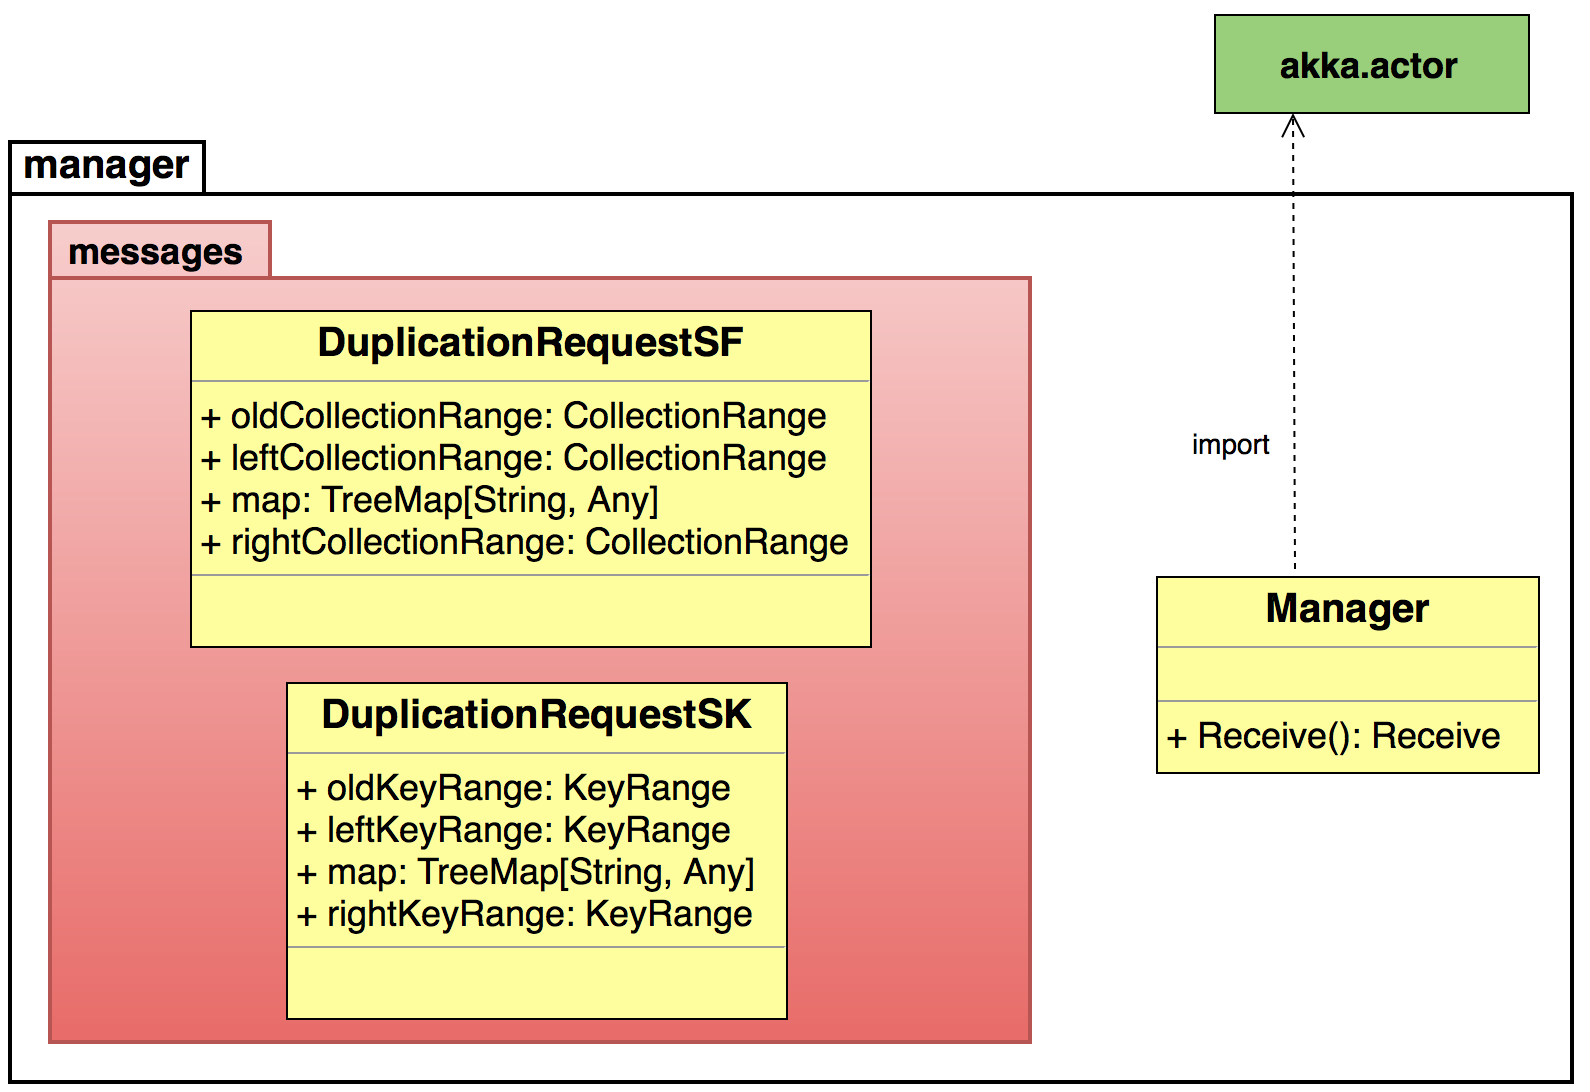
\includegraphics[width=0.8\textwidth,keepaspectratio]{RQ/manager.png}
    \caption{Manager, visione generale del package}
  \end{center}
\end{figure}

\subsubsection{Descrizione}
\gloss{Package} che rappresenta l'\gloss{attore} di tipo \gloss{Manager}.

\subsubsection{Package contenuti}

\begin{itemize}
\item \hyperref[sec:actorbase::actorsystem::manager::messages]{actorbase::actorsystem::manager::messages}.
\end{itemize}

\subsubsection{Classi}

\paragraph{actorbase::actorsystem::manager::Manager}
\label{sec:actorbase::actorsystem::manager::Manager}

\subparagraph{Descrizione}
Classe che rappresenta un \gloss{attore} di tipo \gloss{Manager}.

\subparagraph{Utilizzo}
Questa classe viene utilizzata per gestire le richieste di divisione di attori di tipo
\hyperref[sec:actorbase::actorsystem::storekeeper::Storekeeper]{Storekeeper}
e \hyperref[sec:actorbase::actorsystem::storefinder::Storefinder]{Storefinder}.

\subparagraph{Classi ereditate}
\begin{itemize}
\item akka::actor::Actor.
\end{itemize}

\subparagraph{Attributi}

\begin{tabular}{| p{3cm} | p{1.5cm} | p{2cm} | p{2cm} | p{8.5cm} |}
  \hline
  Nome & Accesso & Mutabilità & Tipo & Descrizione\\
  \hline
  parentRef & private & immutabile & ActorRef & Riferimento all'attore di tipo \gloss{Storefinder} che l'ha creato\\
  \hline
\end{tabular}

\subsection{actorbase::actorsystem::manager::messages}
\label{sec:actorbase::actorsystem::manager::messages}

\subparagraph{Descrizione}
\gloss{Package} che contiene tutti i messaggi che possono essere ricevuti
dall'\gloss{attore} di tipo
\hyperref[sec:actorbase::actorsystem::manager::Manager]{actorbase::\allowbreak{}actorsystem::\allowbreak{}manager::\allowbreak{}Manager}

\paragraph{actorbase::actorsystem::manager::messages::DuplicationRequestSK}
\label{sec:actorbase::actorsystem::manager::messages::DuplicationRequestSK}

\subparagraph{Descrizione}

Messaggio che richiede la divisione a metà dell'\gloss{attore} di tipo
\hyperref[sec:actorbase::actorsystem::storekeeper::Storekeeper]{Storekeeper}.

\subparagraph{Utilizzo}

Quando \hyperref[sec:actorbase::actorsystem::manager::Manager]{Manager}
riceve questo messaggio provvederà a dividere a metà l'\gloss{attore} di tipo
\hyperref[sec:actorbase::actorsystem::storekeeper::Storekeeper]{Storekeeper}
che dovrà essere diviso.\\Manderà inoltre un messaggio \hyperref[sec:actorbase::actorsystem::storefinder::messages::DuplicateSKNotify]{DuplicateSKNotify} all'\gloss{attore} di tipo
\hyperref[sec:actorbase::actorsystem::storefinder::Storefinder]{Storefinder}
per aggiornare i suoi riferimenti.

\subparagraph{Attributi}
\begin{tabular}{| p{3cm} | p{1.5cm} | p{2cm} | p{2cm} | p{8.5cm} |}
  \hline
  Nome & Accesso & Mutabilità & Tipo & Descrizione\\
  \hline
  oldKeyRange & public & immutabile & KeyRange & KeyRange che rappresenta il range di chiavi identificativo da duplicare\\
  \hline
  leftRange & public & immutable & KeyRange & KeyRange che rappresenta il range di chiavi nuovo relativo allo Storekeeper che si è duplicato\\
  \hline
  map & public & immutable & TreeSet [String, Any] & struttura dati da inizializzare allo Storekeeper da creare\\
  \hline
  rightRange & public & immutable & KeyRange & KeyRange che rappresenta il range di chiavi da assegnare allo Storekeeper da creare\\
  \hline
\end{tabular}

\paragraph{actorbase::actorsystem::manager::messages::DuplicationRequestSF}
\label{sec:actorbase::actorsystem::manager::messages::DuplicationRequestSF}

\subparagraph{Descrizione}

Messaggio che richiede la divisione a metà dell'\gloss{attore} di tipo
\gloss{Storefinder}.

\subparagraph{Utilizzo}

Quando \hyperref[sec:actorbase::actorsystem::manager::Manager]{actorbase::\allowbreak{}actorsystem::\allowbreak{}manager::\allowbreak{}Manager}
riceve questo messaggio provvederà a dividere a metà l'\gloss{attore} di tipo
\hyperref[sec:actorbase::actorsystem::storefinder::Storefinder]{actorbase::\allowbreak{}actorsystem::\allowbreak{}storefinder::\allowbreak{}Storefinder}
che dovrà essere diviso. Manderà inoltre un messaggio all'\gloss{attore} di tipo
\hyperref[sec:actorbase::actorsystem::main::Main]{actorbase::\allowbreak{}actorsystem::\allowbreak{}main::\allowbreak{}Main}
per aggiornare i suoi riferimenti.

\subparagraph{Attributi}
\begin{tabular}{| p{3cm} | p{1.5cm} | p{2cm} | p{2cm} | p{8.5cm} |}
  \hline
  Nome & Accesso & Mutabilità & Tipo & Descrizione \\
  \hline
  oldCollRange & public & immutabile & CollectionRange & CollectionRange che identifica quale CollectionRange è da duplicare \\
  \hline
  leftCollRange & public & immutable & CollRange & Identifica il nuovo CollectionRange dello Storefinder che si è duplicato \\
  \hline
  map & public & immutable & TreeSet [KeyRamge, ActorRef] & struttura dati da inizializzare allo Storefinder da creare\\
  \hline
  rightCollRange & public & immutable & CollRange & Identifica il nuovo CollectionRange dello Storefinder da duplicare \\
  \hline
\end{tabular}

%%%%%%%%%%%%%%%%%%%%%%%%%%%%%%%%%%%%%%%%%%%%%%%%%%%%%%%%%%%%%%%%%%%%
%%% DRIVER PARTE                         %%%
%%%%%%%%%%%%%%%%%%%%%%%%%%%%%%%%%%%%%%%%%%%%%%%%%%%%%%%%%%%%%%%%%%%%

\subsection{actorbase::driver}
\label{sec:actorbase::driver}

\begin{figure}[H]
  \begin{center}
    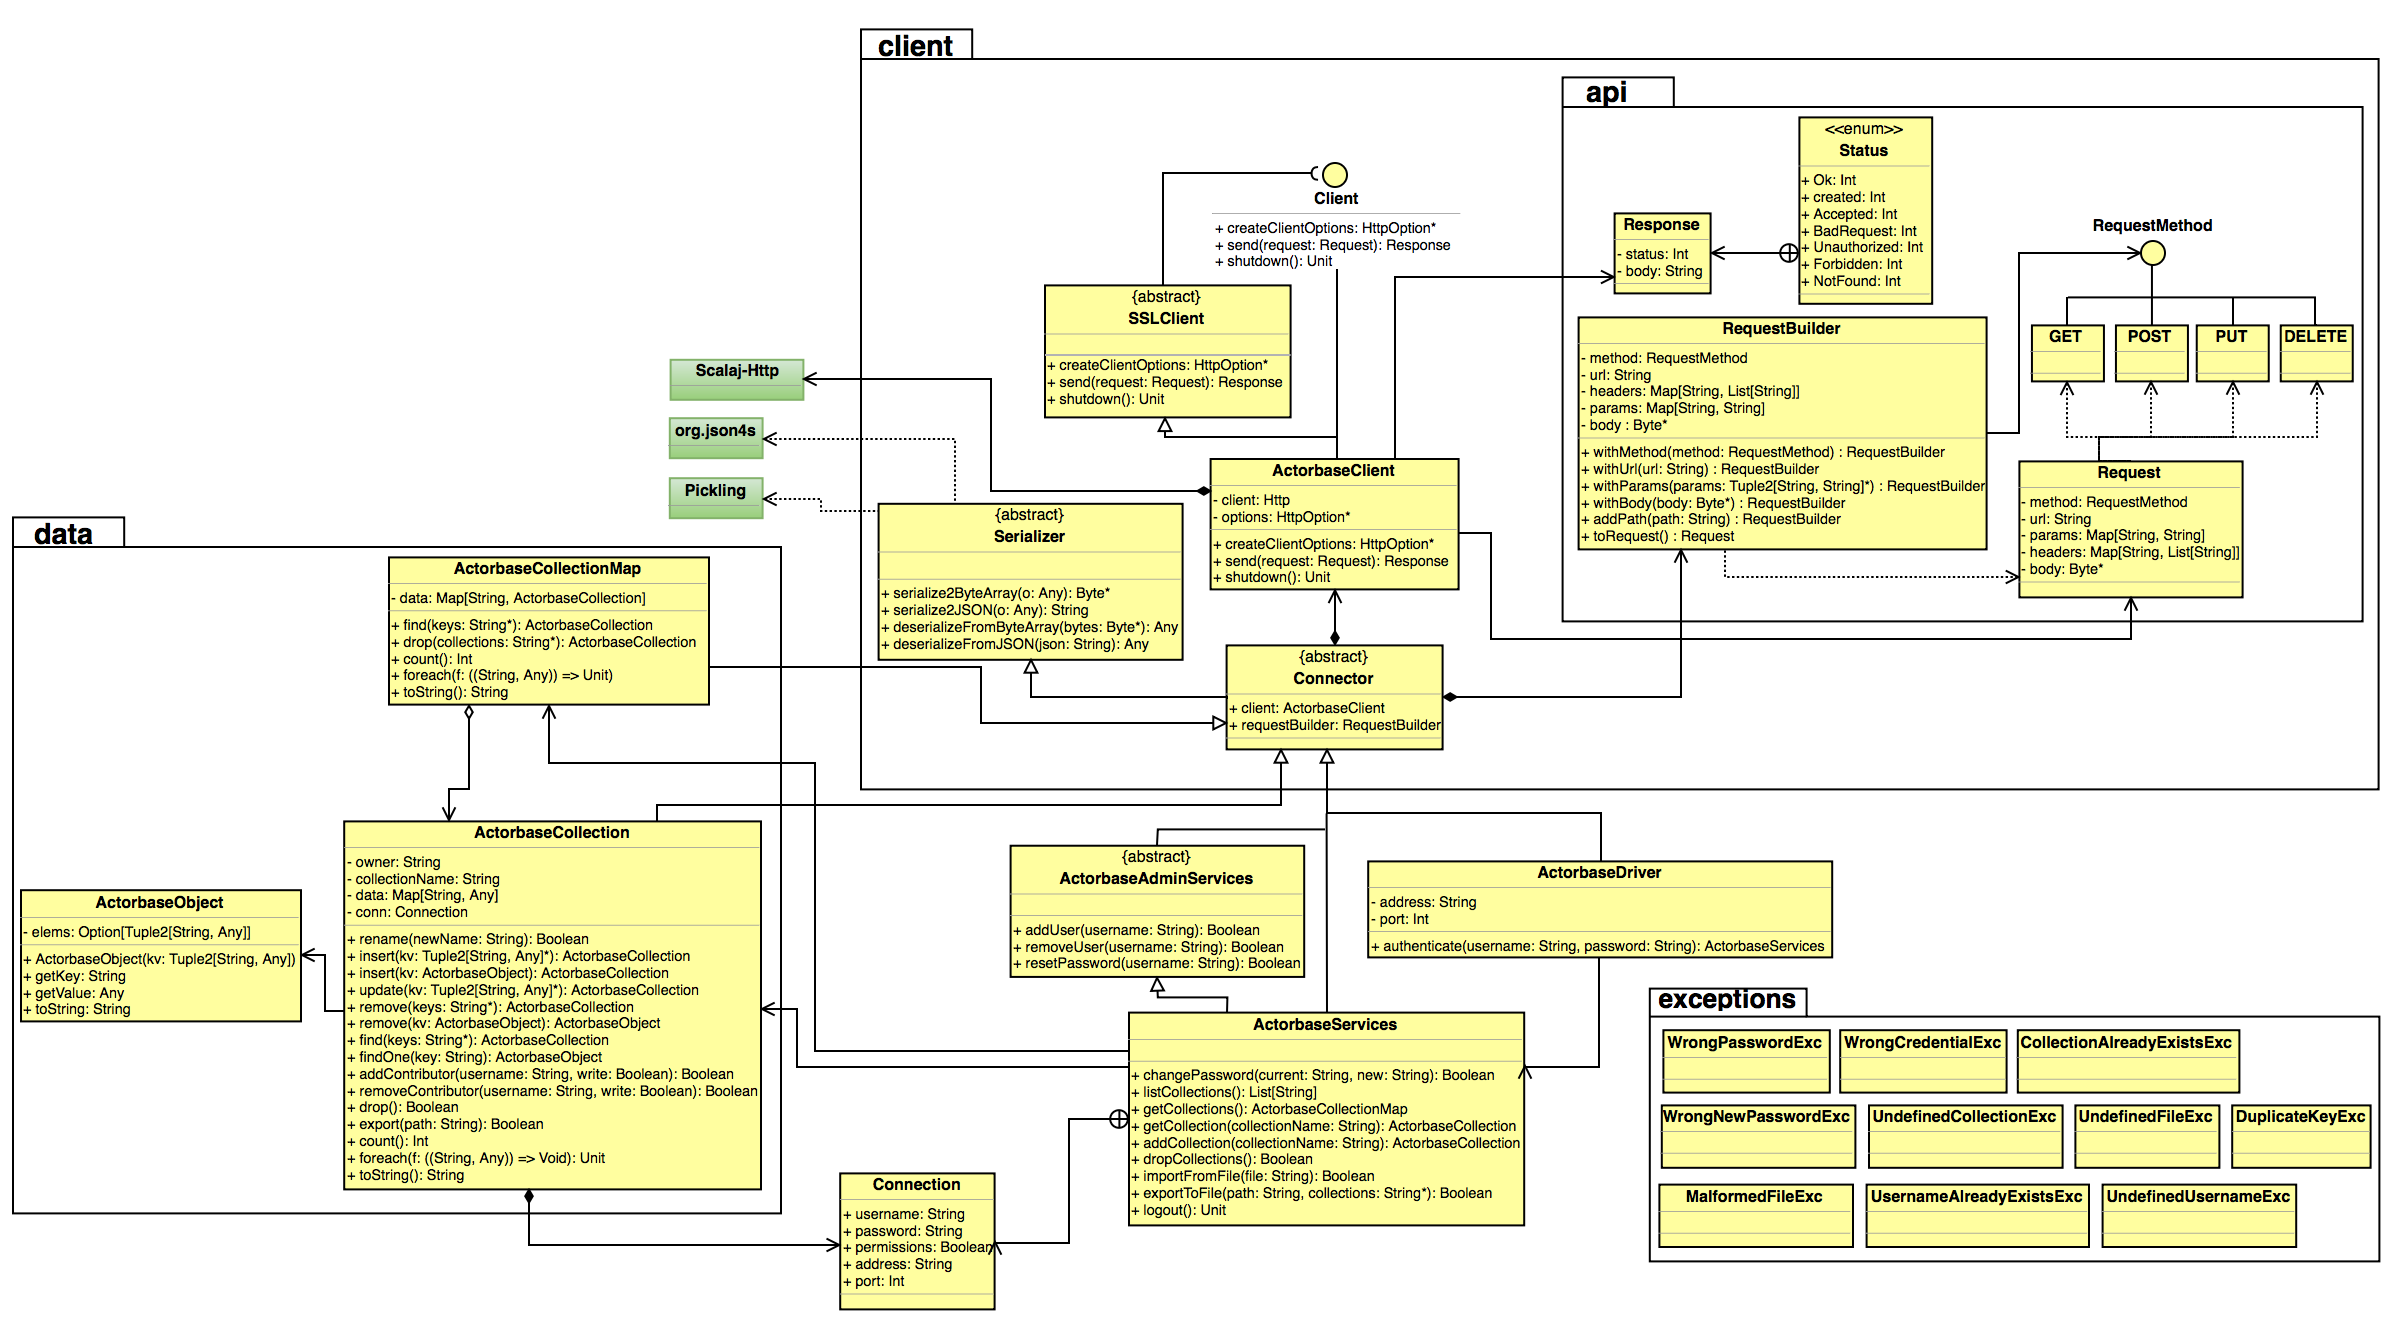
\includegraphics[width=1.0\textwidth,keepaspectratio]{RQ/Driver-RQ.png}
    \caption{Driver: Architettura generale}
  \end{center}
\end{figure}

\subsubsection{Descrizione}

\gloss{Package} per la componente \gloss{driver} da utilizzare in un programma
\gloss{Scala}.

\subsubsection{Package contenuti}

\begin{itemize}
\item \hyperref[sec:actorbase::driver::client]{actorbase::driver::client};
\item \hyperref[sec:actorbase::driver::client::api]{actorbase::driver::client::api};
\item \hyperref[sec:actorbase::driver::data]{actorbase::driver::data};
\item \hyperref[sec:actorbase::driver::exceptions]{actorbase::driver::exceptions}.
\end{itemize}

\subsubsection{Classi}

\paragraph{ActorbaseDriver}
\label{sec:actorbase::driver::ActorbaseDriver}

\begin{figure}[H]
  \begin{center}
    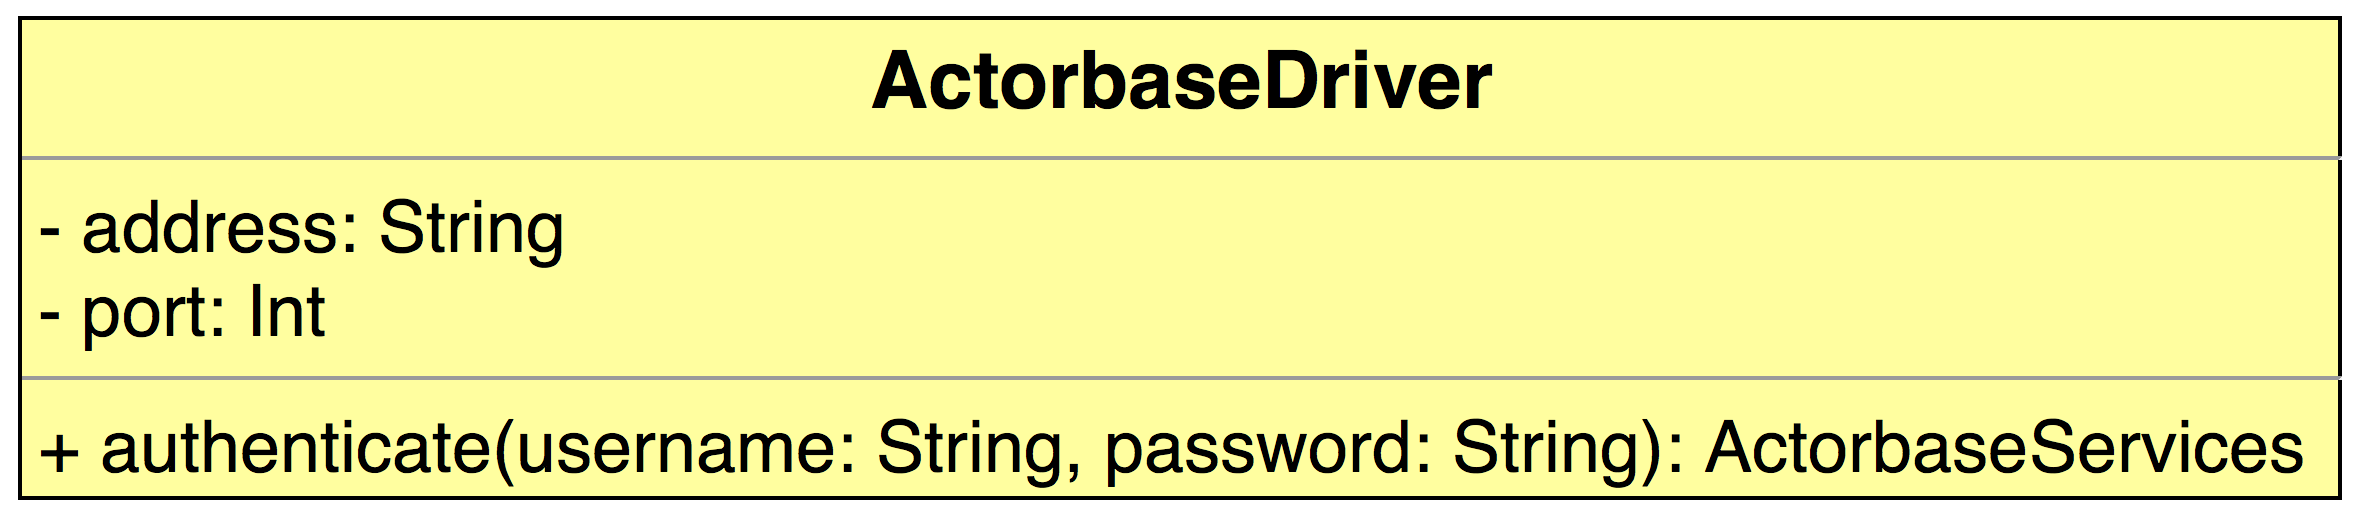
\includegraphics[width=1.0\textwidth,keepaspectratio]{RQ/ActorbaseDriver.png}
    \caption{Driver: Classe ActorbaseDriver}
  \end{center}
\end{figure}

\subparagraph{Descrizione}

Classe principale della componente \gloss{driver}, rappresenta l'interfaccia
di connessione e autenticazione con il \gloss{server}

\subparagraph{Utilizzo}

Espone i metodi di connessione e autenticazione al \gloss{server} \textbf{Actorbase}, e restituisce un oggetto
di tipo \hyperref[sec::actorbase::driver::ActorbaseServices]{ActorbaseServices} in base ai privilegi del proprio
profilo nel sistema.

\subparagraph{Eredita}

\begin{itemize}
\item \hyperref[sec:actorbase::driver::client::Connector]{actorbase::driver::client::Connector}.
\end{itemize}

\subparagraph{Attributi}

% TODO: Da completare

\begin{tabular}{| p{3cm} | p{1.5cm} | p{2cm} | p{2cm} | p{8.5cm} |}
  \hline
  Nome & Accesso & Mutabilità & Tipo & Descrizione\\
  \hline
  address & private & immutabile & String & Rappresenta l'indirizzo del \gloss{server} Actorbase\\
  \hline
  port & private & immutabile & Int & Rappresenta la porta esposta dal \gloss{server}\\
  \hline
\end{tabular}

\subparagraph{Metodi}

% TODO: Da completare

\begin{tabular}{| p{3cm} | p{1.5cm} | p{3cm} | p{10cm} |}
  \hline
  Nome & Accesso & Tipo di ritorno & Descrizione\\
  \hline
  authenticate & public & \hyperref[sec:actorbase::driver::ActorbaseServices]{ActorbaseServices} & Metodo di autenticazione sul server mediante credenziali\\
  \hline
\end{tabular}

\subparagraph{Parametri}

% TODO: Da completare

\begin{center}
  \textbf{authenticate}
\end{center}
\begin{tabular}{| p{3cm} | p{3.5cm} | p{8.5cm} |}
  \hline
  Nome & Tipo & Descrizione\\
  \hline
  username & String & Rappresenta lo \gloss{username} dell'utente\\
  \hline
  password & String & Rappresenta la password dell'utente\\
  \hline
\end{tabular}

\begin{center}
  \textbf{getCollection}
\end{center}
\begin{tabular}{| p{3cm} | p{3.5cm} | p{8.5cm} |}
  \hline
  Nome & Tipo & Descrizione\\
  \hline
  collectionName & String & Rappresenta il nome della \gloss{collezione} da richiedere al server\\
  \hline
\end{tabular}

\begin{center}
  \textbf{addCollection}
\end{center}
\begin{tabular}{| p{3cm} | p{3.5cm} | p{8.5cm} |}
  \hline
  Nome & Tipo & Descrizione\\
  \hline
  collectionName & String & Rappresenta il nome della \gloss{collezione} da richiedere al server\\
  \hline
\end{tabular}

\paragraph{ActorbaseServices}
\label{sec:actorbase::driver::ActorbaseServices}

\begin{figure}[H]
  \begin{center}
    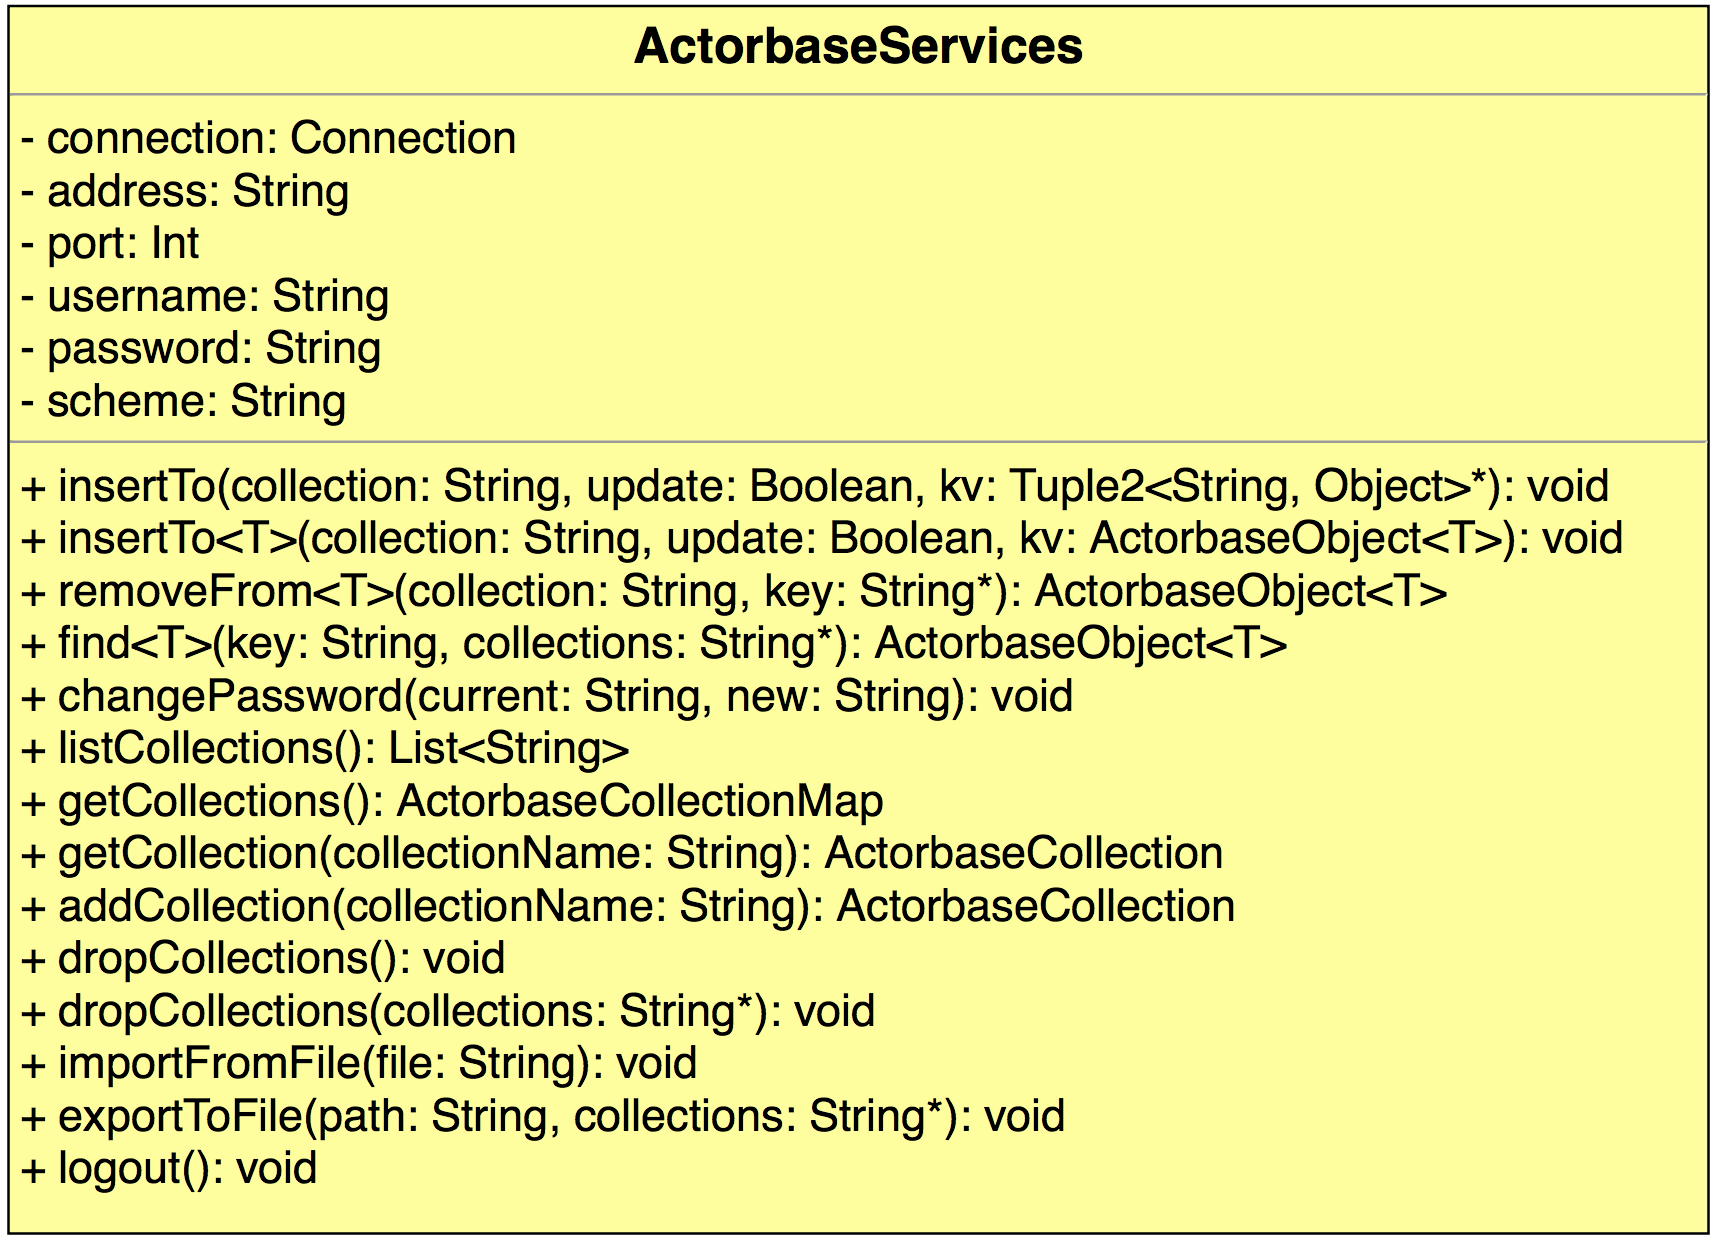
\includegraphics[width=1.0\textwidth,keepaspectratio]{RQ/ActorbaseServices.png}
    \caption{Driver: Classe ActorbaseServices}
  \end{center}
\end{figure}

\subparagraph{Descrizione}

Classe principale della componente \gloss{driver}, rappresenta l'interfaccia
contenente i metodi designati all'utilizzo di \textbf{Actorbase} in un programma
\gloss{Scala}.

\subparagraph{Utilizzo}

Espone i metodi di interrogazione, ricerca e gestione dei dati
remoti all'interno del \gloss{database}.

\subparagraph{Eredita}

\begin{itemize}
\item \hyperref[sec:actorbase::driver::client::Connector]{actorbase::driver::client::Connector}.
\item \hyperref[sec:actorbase::driver::ActorbaseAdminServices]{actorbase::driver::ActorbaseAdminServices}.
\end{itemize}

\subparagraph{Metodi}

% TODO: Da completare

\begin{tabular}{| p{3cm} | p{1.5cm} | p{3cm} | p{9.5cm} |}
  \hline
  Nome & Accesso & Tipo di ritorno & Descrizione\\
  \hline
  changePassword & public & Boolean & Metodo utilizzato per la modifica della propria password di profilo \textbf{Actorbase}\\
  \hline
  listCollections & public & List[String] & Ritorna una lista di stringhe, rappresentano i nomi delle collezioni\\
  \hline
  getCollections & public & \hyperref[sec:actorbase::driver::data::ActorbaseCollectionMap]{ActorbaseCollection\allowbreak{}Map} & Ritorna un oggetto di tipo \hyperref[sec:actorbase::driver::data::ActorbaseCollectionMap]{ActorbaseCollectionMap}\\
  \hline
  getCollection & public & \hyperref[sec:actorbase::driver::data::ActorbaseCollection]{ActorbaseCollection} & Ritorna un oggetto di tipo \hyperref[sec:actorbase::driver::data::ActorbaseCollection]{ActorbaseCollection}\\
  \hline
  addCollection & public & \hyperref[sec:actorbase::driver::data::ActorbaseCollection]{ActorbaseCollection} & Ritorna un oggetto di tipo \hyperref[sec:actorbase::driver::data::ActorbaseCollection]{ActorbaseCollection}\\
  \hline
  dropCollection & public & \hyperref[sec:actorbase::driver::data::ActorbaseCollection]{ActorbaseCollection} & Ritorna un oggetto di tipo \hyperref[sec:actorbase::driver::data::ActorbaseCollection]{ActorbaseCollection}\\
  \hline
  importFromFile & public & Boolean & Metodo da utilizzare per importare \gloss{collezioni} sul \gloss{server} da \gloss{file}\\
  \hline
  exportToFile & public & Boolean & Metodo da utilizzare per esportare \gloss{collezioni} dal \gloss{server} su \gloss{filesystem}\\
  \hline
  logout & public & Unit & Effettua il logout dal server\\
  \hline
\end{tabular}

\subparagraph{Parametri}

% TODO: Da completare

\begin{center}
  \textbf{changePassword}
\end{center}
\begin{tabular}{| p{3cm} | p{3.5cm} | p{8.5cm} |}
  \hline
  Nome & Tipo & Descrizione\\
  \hline
  current & String & Rappresenta la password attuale sul profilo \textbf{Actorbase}\\
  \hline
  new & String & Rappresenta la nuova password di profilo \textbf{Actorbase}\\
  \hline
\end{tabular}

\begin{center}
  \textbf{getCollection}
\end{center}
\begin{tabular}{| p{3cm} | p{3.5cm} | p{8.5cm} |}
  \hline
  Nome & Tipo & Descrizione\\
  \hline
  collectionName & String & Rappresenta il nome della \gloss{collezione} da richiedere al \gloss{server}\\
  \hline
\end{tabular}

\begin{center}
  \textbf{addCollection}
\end{center}
\begin{tabular}{| p{3cm} | p{3.5cm} | p{8.5cm} |}
  \hline
  Nome & Tipo & Descrizione\\
  \hline
  collectionName & String & Rappresenta il nome della \gloss{collezione} da richiedere al \gloss{server}\\
  \hline
\end{tabular}

\begin{center}
  \textbf{importFromFile}
\end{center}
\begin{tabular}{| p{3cm} | p{3.5cm} | p{8.5cm} |}
  \hline
  Nome & Tipo & Descrizione\\
  \hline
  path & String & Rappresenta il percorso su \gloss{filesystem} del \gloss{file} contenente le \gloss{collezioni} da importare sul \gloss{server}\\
  \hline
\end{tabular}

\begin{center}
  \textbf{exportToFile}
\end{center}
\begin{tabular}{| p{3cm} | p{3.5cm} | p{8.5cm} |}
  \hline
  Nome & Tipo & Descrizione\\
  \hline
  path & String & Rappresenta il percorso su \gloss{filesystem} del \gloss{file} da utilizzare per l'esportazione delle \gloss{collezioni} dal \gloss{server}\\
  \hline
  collections & \gloss{vararg} di String & Rappresenta una sequenza eventualmente vuota di nomi di \gloss{collezioni} da esportare su \gloss{filesystem}.\\
  \hline
\end{tabular}

% FINE ACTORBASEDRIVER

\paragraph{ActorbaseAdminServices (abstract)}
\label{sec:actorbase::driver::ActorbaseAdminServices}

\begin{figure}[H]
  \begin{center}
    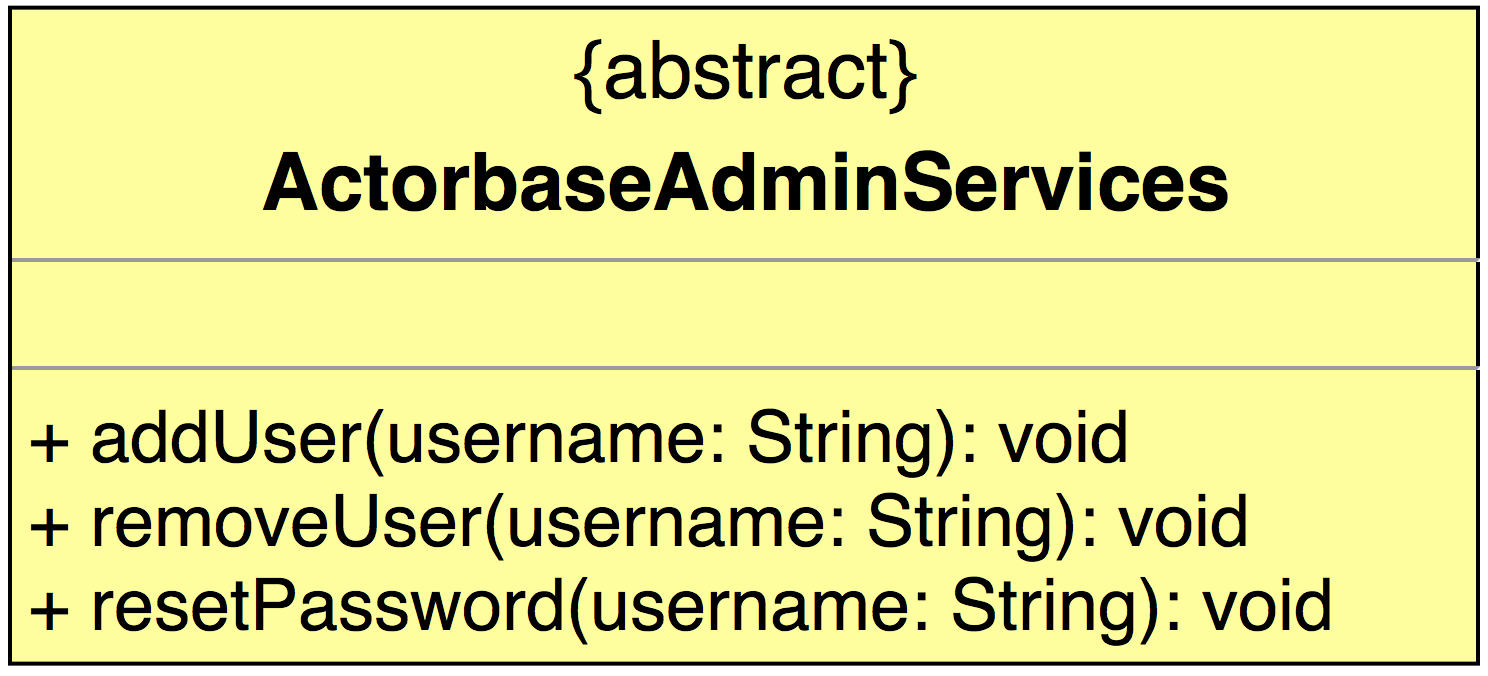
\includegraphics[width=1.0\textwidth,keepaspectratio]{RQ/ActorbaseAdminServices.png}
    \caption{Driver: Classe ActorbaseAdminServices}
  \end{center}
\end{figure}

\subparagraph{Descrizione}

Classe astratta contenente alcuni metodi di utilità esclusivamente amministrativa.

\subparagraph{Utilizzo}

Aggiunge funzionalità amministrative all'oggetto
\hyperref[sec:actorbase::driver::ActorbaseServices]{ActorbaseServices}, ossia
operazioni di gestione degli utenti. Funge da iniezione di dipendenze mediante
\gloss{cake pattern}.

\subparagraph{Eredita}

\begin{itemize}
\item \hyperref[sec:actorbase::driver::client::Connector]{actorbase::driver::client::Connector}.
\end{itemize}

\subparagraph{Metodi}

% TODO: Da completare

\begin{tabular}{| p{3cm} | p{1.5cm} | p{2.5cm} | p{10cm} |}
  \hline
  Nome & Accesso & Tipo di ritorno & Descrizione\\
  \hline
  addUSer & public & Boolean & Permette di aggiungere un nuovo utente al sistema\\
  \hline
  removeUser & public & Boolean & Permette la rimozione di un utente dal sistema\\
  \hline
  resetPassword & public & Boolean & Effettua il \gloss{reset} della password di un utente\\
  \hline
\end{tabular}

\subparagraph{Parametri}

% TODO: Da completare

\begin{center}
  \textbf{addUser}
\end{center}
\begin{tabular}{| p{3cm} | p{3.5cm} | p{8.5cm} |}
  \hline
  Nome & Tipo & Descrizione\\
  \hline
  username & String & Rappresenta lo \gloss{username} dell'utente da aggiungere al sistema\\
  \hline
\end{tabular}

\begin{center}
  \textbf{removeUser}
\end{center}
\begin{tabular}{| p{3cm} | p{3.5cm} | p{8.5cm} |}
  \hline
  Nome & Tipo & Descrizione\\
  \hline
  username & String & Rappresenta lo \gloss{username} dell'utente da rimuovere dal sistema\\
  \hline
\end{tabular}

\begin{center}
  \textbf{resetPassword}
\end{center}
\begin{tabular}{| p{3cm} | p{3.5cm} | p{8.5cm} |}
  \hline
  Nome & Tipo & Descrizione\\
  \hline
  username & String & Rappresenta lo \gloss{username} dell'utente a cui effettuare il \gloss{reset} della password\\
  \hline
\end{tabular}

% FINE ACTORBASEADMINSERVICES

\paragraph{Connection}
\label{sec:actorbase::driver::Connection}

\begin{figure}[H]
  \begin{center}
    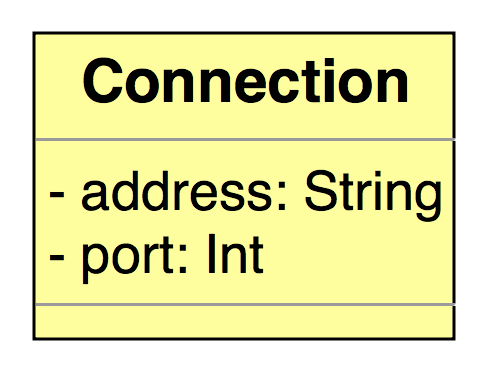
\includegraphics[width=1.0\textwidth,keepaspectratio]{RQ/Connection.png}
    \caption{Driver: Classe Connection}
  \end{center}
\end{figure}

\subparagraph{Descrizione}

Classe interna all'oggetto
\hyperref[sec:actorbase::driver::ActorbaseServices]{ActorbaseServices} contenente i
parametri di connessione al \gloss{server} e le credenziali del profilo \textbf{Actorbase}.

\subparagraph{Utilizzo}

Viene utilizzata come oggetto contenente i parametri di connessione, da
utilizzare nelle classi che necessitano di collegamenti al \gloss{server}.

\subparagraph{Attributi}

\begin{tabular}{| p{3cm} | p{1.5cm} | p{2cm} | p{2cm} | p{8.5cm} |}
  \hline
  Nome & Accesso & Mutabilità & Tipo & Descrizione\\
  \hline
  username & public & immutabile & String & Rappresenta lo \gloss{username} dell'utente\\
  \hline
  password & public & immutabile & String & Rappresenta la password dell'utente\\
  \hline
  administrator & public & immutabile & Boolean & Indica il livello di privilegio del profilo \textbf{Actorbase}, \gloss{true} se amministrativo, altrimento \gloss{false}\\
  \hline
  address & public & immutabile & String & Rappresenta l'indirizzo del \gloss{server} \textbf{Actorbase}\\
  \hline
  port & public & immutabile & Int & Rappresenta la porta esposta dal \gloss{server}\\
  \hline
\end{tabular}

\subsection{actorbase::driver::client}
\label{sec:actorbase::driver::client}

\begin{figure}[H]
  \begin{center}
    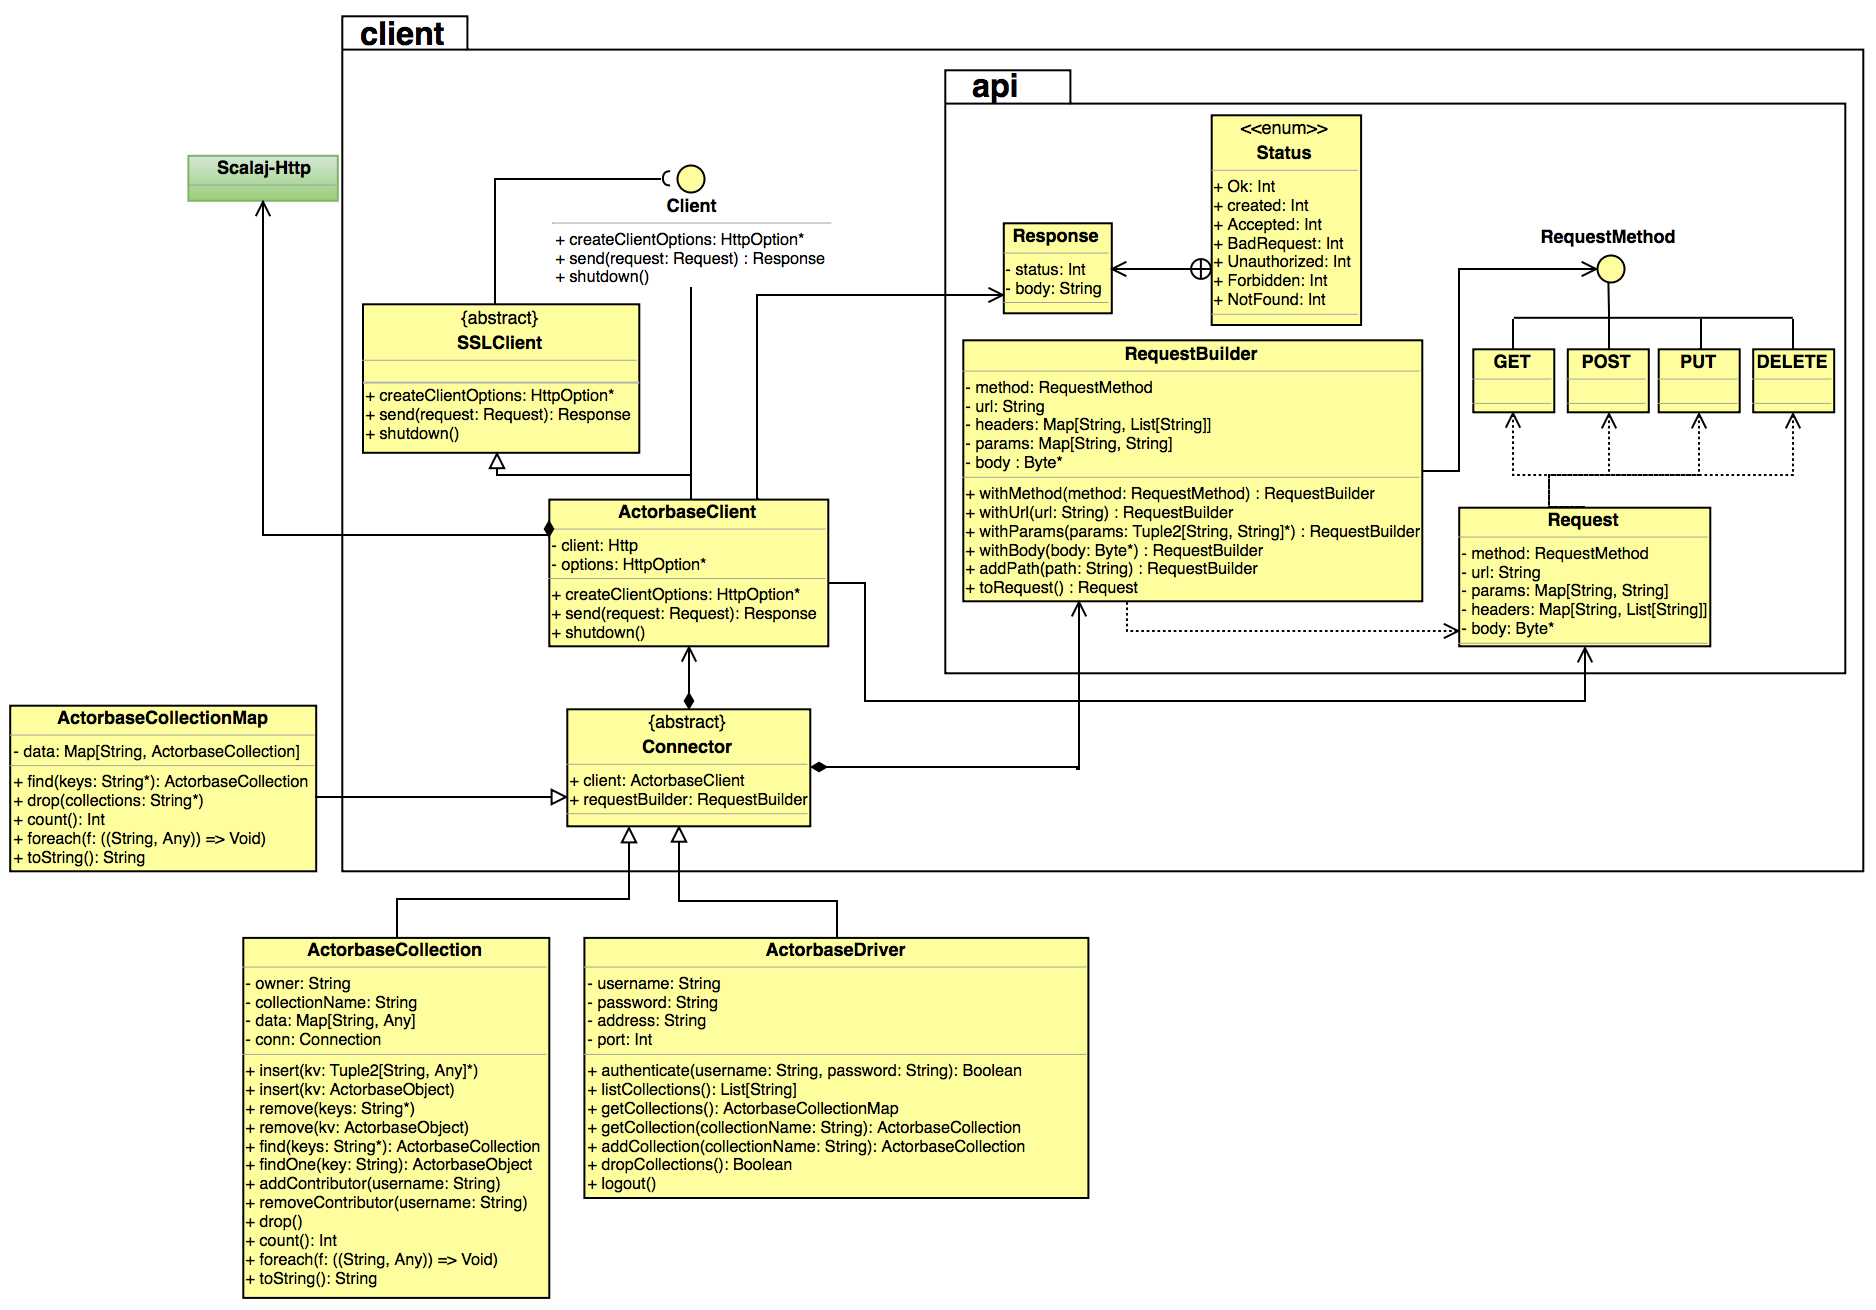
\includegraphics[width=1.0\textwidth,keepaspectratio]{RQ/Client.png}
    \caption{Driver: Client}
  \end{center}
\end{figure}

\subsubsection{Descrizione}

\gloss{Package} che si occupa di comunicare sia con la componente \gloss{cli}
che con la componente \gloss{server} del sistema.

\subsubsection{Interfacce}

\paragraph{Client}
\label{sec:actorbase::driver::client::Client}

\begin{figure}[H]
  \begin{center}
    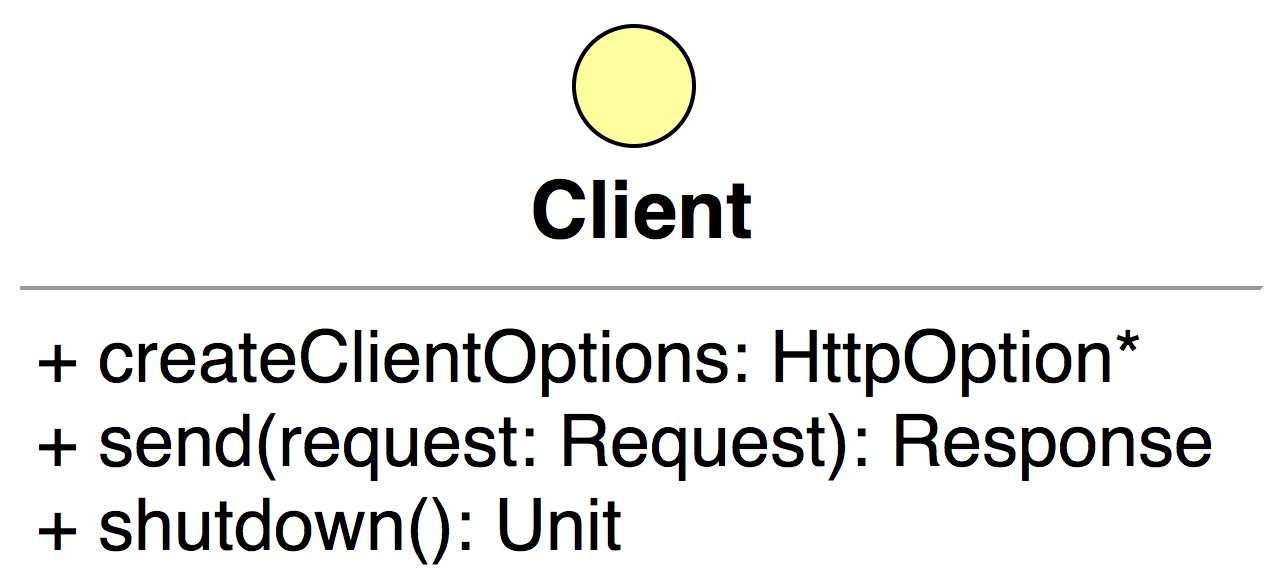
\includegraphics[width=0.9\textwidth,keepaspectratio]{RQ/ClientInterface.png}
    \caption{Driver: Client interface}
  \end{center}
\end{figure}

\subparagraph{Descrizione}

Interfaccia che rappresenta il comportamento di un client atto alla connessione con un server.

\subparagraph{Utilizzo}

Viene utilizzata per delineare il comportamento generale di un generico client,
le classi che la realizzano hanno libertà di implementazione specifica dei
metodi.

\subparagraph{Ereditata da}

\begin{itemize}
\item \hyperref[sec:actorbase::driver::client::SSLClient]{actorbase::driver::client::SSLClient}
\end{itemize}

\subparagraph{Realizzata da}

\begin{itemize}
\item \hyperref[sec:actorbase::driver::client::ActorbaseClient]{actorbase::driver::client::ActorbaseClient}
\end{itemize}

\subparagraph{Metodi}

\begin{tabular}{| p{3cm} | p{1.5cm} | p{2.5cm} | p{10cm} |}
  \hline
  Nome & Accesso & Tipo di ritorno & Descrizione\\
  \hline
  createClientOptions & public & \gloss{array} di HttpOption & Crea le opzioni di utilizzo del \gloss{client} \gloss{Http}\\
  \hline
  send & public & \hyperref[sec::actorbase::driver::client::api]{Response} & Invia la richiesta al server e riceve la risposta sincronamente\\
  \hline
  shutdown & public & Unit  & Chiude la connessione con il server\\
  \hline
\end{tabular}

\subparagraph{Parametri}

\begin{center}
  \textbf{send}
\end{center}
\begin{tabular}{| p{3cm} | p{3.5cm} | p{8.5cm} |}
  \hline
  Nome & Tipo & Descrizione\\
  \hline
  request & \hyperref[actorbase::driver::client::api::Request]{Request} & Rappresenta una richiesta da inviare al server, comprensiva di \gloss{payload} dati\\
  \hline
\end{tabular}

\subsubsection{Classi}

\paragraph{Serializer (abstract)}
\label{sec:actorbase::driver::client::Serializer}

\begin{figure}[H]
  \begin{center}
    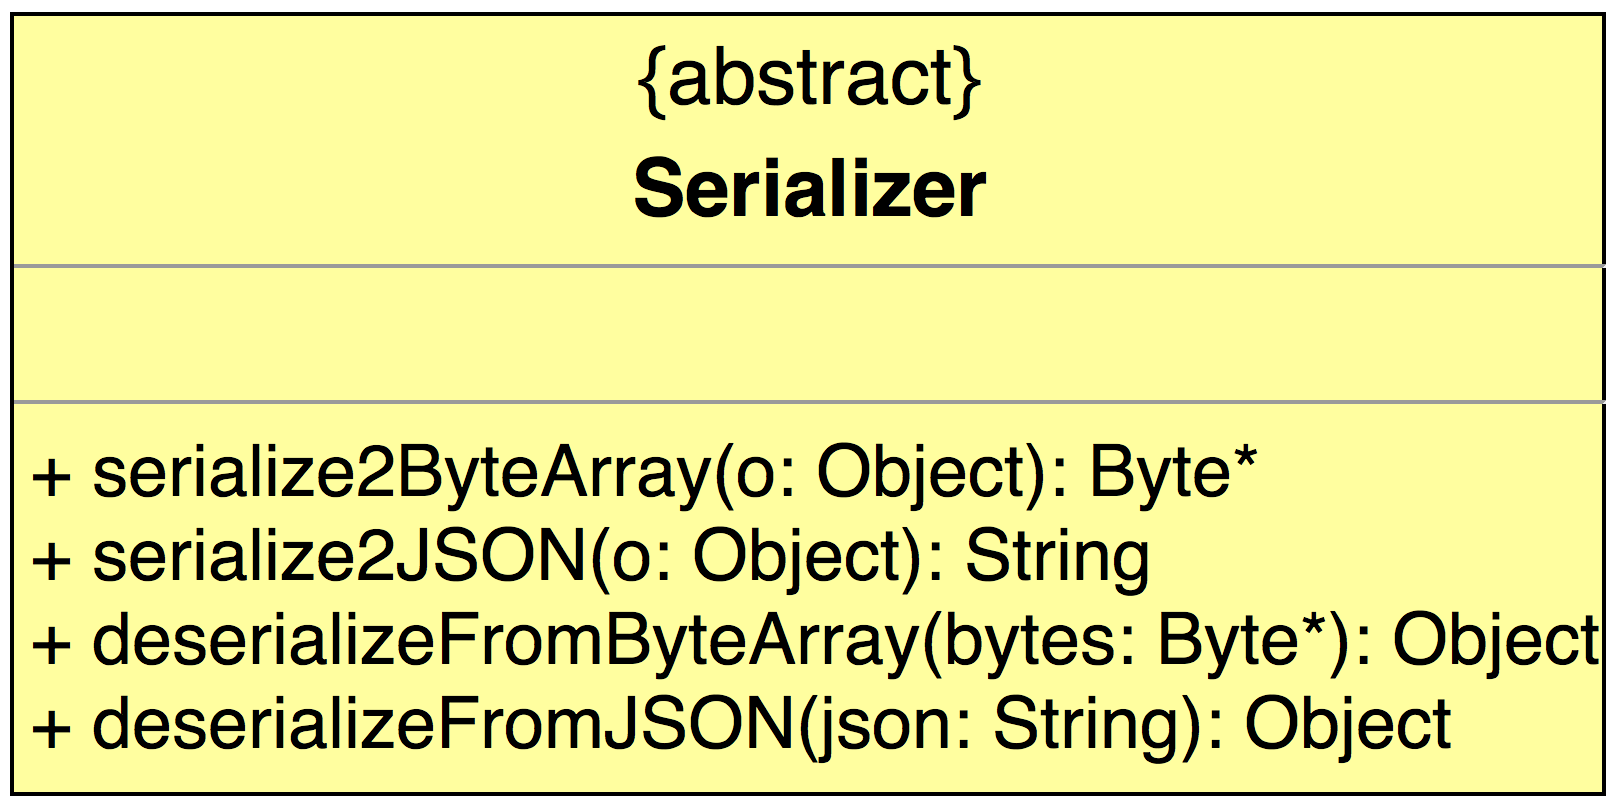
\includegraphics[width=0.9\textwidth,keepaspectratio]{RQ/Serializer.png}
    \caption{Driver: Classe serializer}
  \end{center}
\end{figure}


\subparagraph{Descrizione}

Classe astratta atta a fornire metodi di serializzazione e deserializzazione nelle
varianti \gloss{JSON} e \gloss{array} di \gloss{byte}.

\subparagraph{Utilizzo}

Viene utilizzata mediante estensione dalle classi che necessitano di operazioni di
serializzazione e deserializzazione in formato \gloss{JSON} o \gloss{array} di byte
o entrambi.

\subparagraph{Ereditata da}
% TODO controllare eventuali altre eredità
\begin{itemize}
\item \hyperref[sec:actorbase::driver::client::Connector]{actorbase::driver::client::Connector}.
\end{itemize}

\subparagraph{Metodi}

\begin{tabular}{| p{3cm} | p{1.5cm} | p{2.5cm} | p{10cm} |}
  \hline
  Nome & Accesso & Tipo di ritorno & Descrizione\\
  \hline
  serialize2ByteArray & public & \gloss{array} di \gloss{Byte} & Serializza l'oggetto parametro in formato \gloss{array} di \gloss{Byte}\\
  \hline
  serialize2JSON & public & String & Serializza l'oggetto parametro in formato \gloss{JSON}\\
  \hline
  deserializeFrom\allowbreak{}ByteArray & public & \gloss{Any} & Deserializza l'\gloss{array} di \gloss{Byte} parametro riportandolo al formato originale\\
  \hline
  deserializeFrom\allowbreak{}JSON & public & \gloss{Any} & Deserializza la stringa \gloss{JSON} parametro riportandola al formato originale\\
  \hline
\end{tabular}

\subparagraph{Parametri}

\begin{center}
  \textbf{serialize2Bytearray}
\end{center}
\begin{tabular}{| p{3cm} | p{3.5cm} | p{8.5cm} |}
  \hline
  Nome & Tipo & Descrizione\\
  \hline
  o & \gloss{Any} & L'oggetto generico da serializzare in formato \gloss{array} di \gloss{byte}\\
  \hline
\end{tabular}

\begin{center}
  \textbf{serialize2JSON}
\end{center}
\begin{tabular}{| p{3cm} | p{3.5cm} | p{8.5cm} |}
  \hline
  Nome & Tipo & Descrizione\\
  \hline
  o & \gloss{Any} & L'oggetto generico da serializzare in formato \gloss{JSON}\\
  \hline
\end{tabular}

\begin{center}
  \textbf{deserializeFromByteArray}
\end{center}
\begin{tabular}{| p{3cm} | p{3.5cm} | p{8.5cm} |}
  \hline
  Nome & Tipo & Descrizione\\
  \hline
  bytes & \gloss{array} di \gloss{Byte} & Rappresentazione di un' oggetto serializzato in formato \gloss{array} di \gloss{byte}\\
  \hline
\end{tabular}

\begin{center}
  \textbf{deserializeFromJSON}
\end{center}
\begin{tabular}{| p{3cm} | p{3.5cm} | p{8.5cm} |}
  \hline
  Nome & Tipo & Descrizione\\
  \hline
  json & String & Rappresentazione di un' oggetto serializzato in formato \gloss{JSON}\\
  \hline
\end{tabular}

% FINE SERIALIZER

\paragraph{SSLClient (abstract)}
\label{sec:actorbase::driver::client::SSLClient}

\begin{figure}[H]
  \begin{center}
    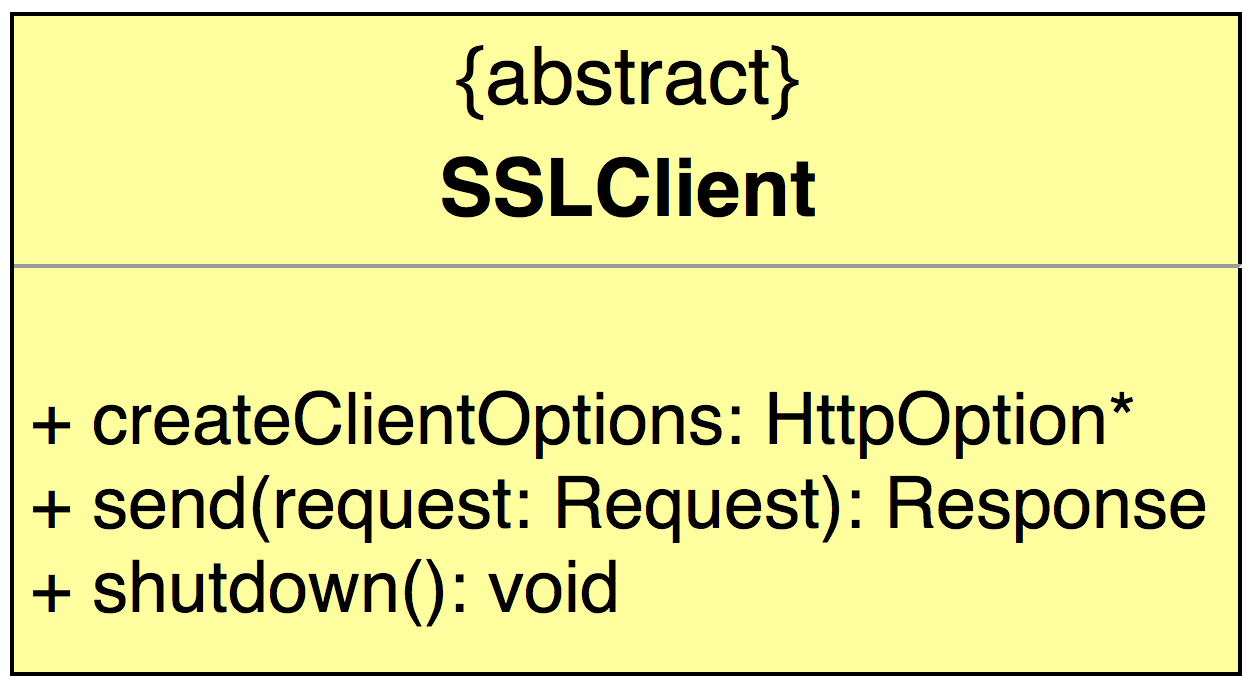
\includegraphics[width=0.9\textwidth,keepaspectratio]{RQ/SSLClient.png}
    \caption{Driver: Classe SSLClient}
  \end{center}
\end{figure}

\subparagraph{Descrizione}

Classe astratta che rappresenta il comportamento di un client atto alla connessione
protetta con un server.

\subparagraph{Utilizzo}

Viene utilizzata per delineare il comportamento generale di un generico client,
funge da \gloss{Decorator} in quanto aggiunge funzionalità di protezione della
connesione mediante protocolli \gloss{TLS/SSL}, le classi che la realizzano
hanno libertà di implementazione specifica dei metodi.

\subparagraph{Realizzata da}

\begin{itemize}
\item \hyperref[sec:actorbase::driver::client::ActorbaseClient]{actorbase::driver::client::ActorbaseClient}
\end{itemize}

\subparagraph{Metodi}

\begin{tabular}{| p{3cm} | p{1.5cm} | p{2.5cm} | p{10cm} |}
  \hline
  Nome & Accesso & Tipo di ritorno & Descrizione\\
  \hline
  createClientOptions & public & \gloss{array} di HttpOption & Crea le opzioni di utilizzo del \gloss{client} \gloss{Http} specificandone il protocollo di protezione\\
  \hline
  send & public & \hyperref[sec:actorbase::driver::client::api::Response]{Response} & Invia la richiesta al server e riceve la risposta sincronamente\\
  \hline
  shutdown & public & Unit  & Chiude la connessione con il server\\
  \hline
\end{tabular}

\subparagraph{Parametri}

\begin{center}
  \textbf{send}
\end{center}
\begin{tabular}{| p{3cm} | p{3.5cm} | p{8.5cm} |}
  \hline
  Nome & Tipo & Descrizione\\
  \hline
  request & \hyperref[actorbase::driver::client::api::Request]{Request} & Rappresenta una richiesta da inviare al server, comprensiva di \gloss{payload} dati\\
  \hline
\end{tabular}

\paragraph{ActorbaseClient}
\label{sec:actorbase::driver::client::ActorbaseClient}

\begin{figure}[H]
  \begin{center}
    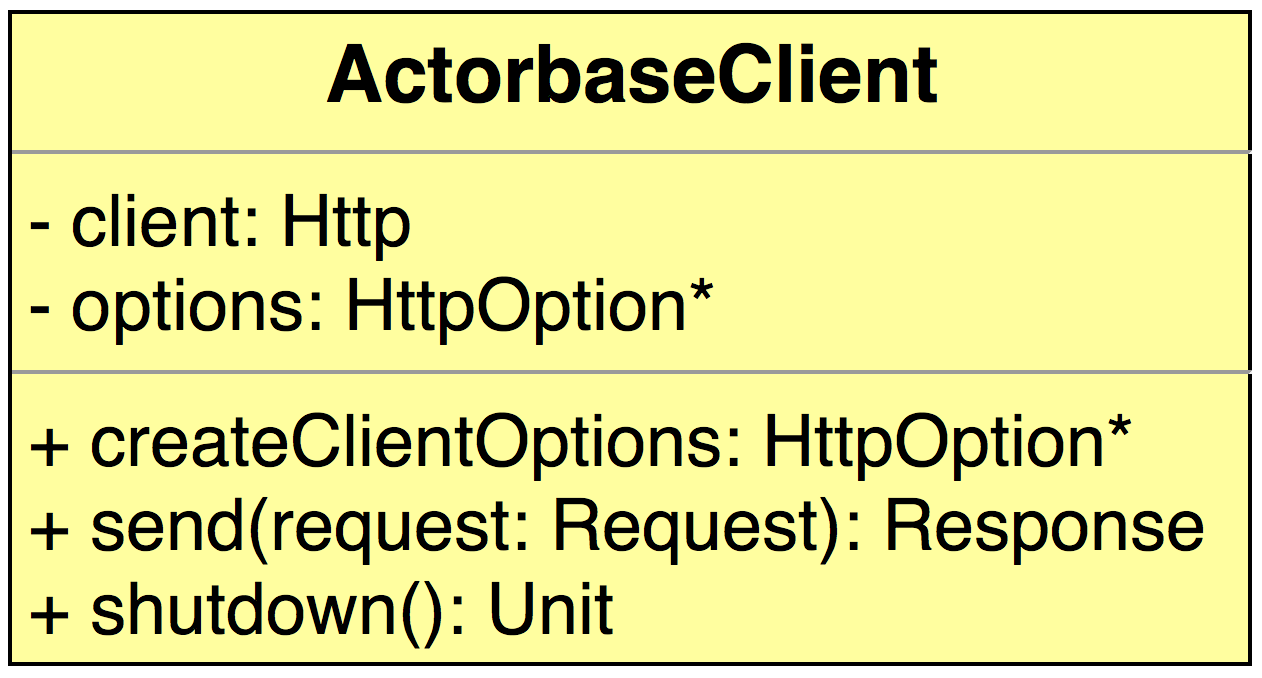
\includegraphics[width=0.9\textwidth,keepaspectratio]{RQ/ActorbaseClient.png}
    \caption{Driver: Classe ActorbaseClient}
  \end{center}
\end{figure}

\subparagraph{Descrizione}

Classe che rappresenta il client utilizzato per la connessione con la componente
\gloss{server} del sistema.

\subparagraph{Utilizzo}

Viene utilizzata dalla componente
\hyperref[sec:actorbase::driver::client::Connector]{Connector} per fornire la
comunicazione con la componente \gloss{server} del sistema alle classi che lo
necessitano.

\subparagraph{Interfacce realizzate}

\begin{itemize}
\item \hyperref[sec:actorbase::driver::client::Client]{actorbase::driver::client::Client}.
\end{itemize}

\subparagraph{Classi ereditate}

\begin{itemize}
\item \hyperref[sec:actorbase::driver::client::SSLClient]{actorbase::driver::client::SSLClient}.
\end{itemize}

\subparagraph{Attributi}

\begin{tabular}{| p{3cm} | p{1.5cm} | p{2cm} | p{2cm} | p{8.5cm} |}
  \hline
  Nome & Accesso & Mutabilità & Tipo & Descrizione\\
  \hline
  client & private & immutabile & Http & Oggetto istanziato utilizzando la libreria esterna \gloss{Scalaj} dedicato alla comunicazione \gloss{HTTP} con il server\\
  \hline
  options & private & immutabile & array di HttpOption & Array di opzioni da utilizzare con l'oggetto client, responsabile di settaggi quali livello di protezione della comunicazione e \gloss{timeout} richieste\\
  \hline
\end{tabular}

\subparagraph{Metodi}

\begin{tabular}{| p{3cm} | p{1.5cm} | p{2.5cm} | p{10cm} |}
  \hline
  Nome & Accesso & Tipo di ritorno & Descrizione\\
  \hline
  createClientOptions & public & \gloss{array} di HttpOption & Crea le opzioni di utilizzo del \gloss{client} \gloss{Http}\\
  \hline
  send & public & \hyperref[sec::actorbase::driver::api::Response]{Response} & Invia la richiesta al server e riceve la risposta sincronamente\\
  \hline
  shutdown & public &  & Chiude la connessione con il server\\
  \hline
\end{tabular}

% FINE ACTORBASECLIENT

\paragraph{Connector (abstract)}
\label{sec:actorbase::driver::client::Connector}

\begin{figure}[H]
  \begin{center}
    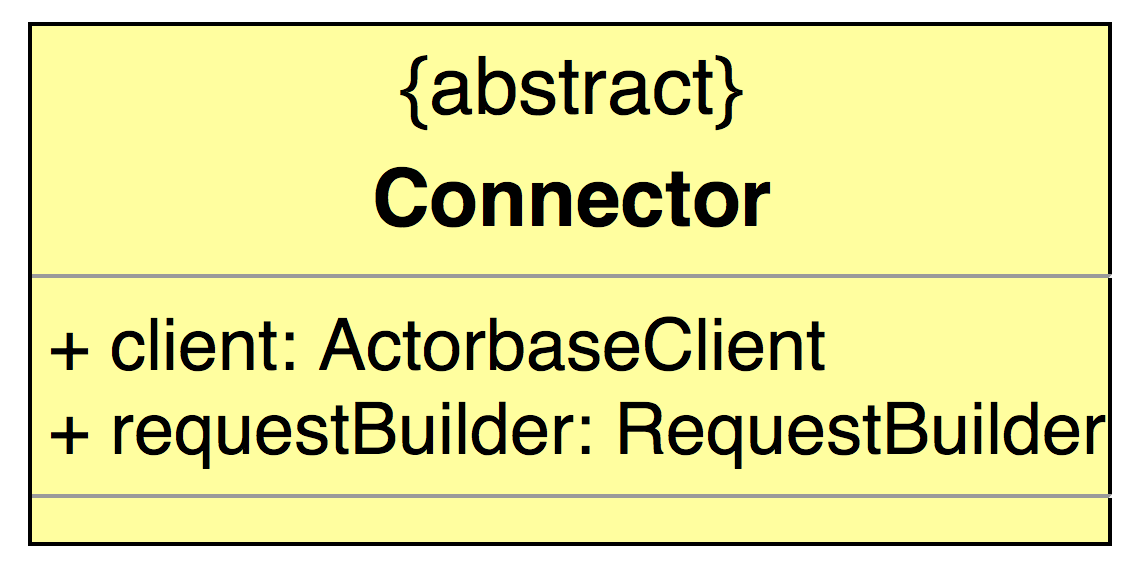
\includegraphics[width=0.9\textwidth,keepaspectratio]{RQ/Connector.png}
    \caption{Driver: Classe astratta Connector}
  \end{center}
\end{figure}

\subparagraph{Descrizione}

Classe astratta che si occupa di istanziare un oggetto di tipo
\hyperref[sec:actorbase::driver::client::ActorbaseClient]{ActorbaseClient} e uno
di tipo
\hyperref[sec:actorbase::driver::client::api::RequestBuilder]{RequestBuilder} in
modo da fornire possibilità di comunicazione con il server alle classi che la
estendono.

\subparagraph{Utilizzo}

Viene estesa dalle classi che necessitano di comunicare con il server.

\subparagraph{Attributi}

\begin{tabular}{| p{3cm} | p{1.5cm} | p{2cm} | p{2.5cm} | p{8cm} |}
  \hline
  Nome & Accesso & Mutabilità & Tipo & Descrizione\\
  \hline
  client & public & immutabile & \hyperref[sec:actorbase::driver::ActorbaseClient]{ActorbaseClient} & Ha lo scopo di fornire comunicazione con il server, mediante protocollo \gloss{HTTP}\\
  \hline
  requestBuilder & public & immutabile & \hyperref[sec:actorbase::driver::api::RequestBuilder]{RequestBuilder} & E' utilizzato per costruire le richieste \gloss{REST} da iniviare al server mediante oggetto di tipo \hyperref[sec:actorbase::driver::client::api::Request]{Request}\\
  \hline
\end{tabular}

\subparagraph{Eredita}
\begin{itemize}
\item \hyperref[sec:actorbase::driver::client::Serializer]{actorbase::driver::client::Serializer}.
\end{itemize}

\subparagraph{Ereditata da}
\begin{itemize}
\item \hyperref[sec:actorbase::driver::client::Connector]{actorbase::driver::client::Connector}.
\end{itemize}

% FINE CONNECTOR

% INIZIO PACKAGE ACTORBASE::DRIVER::CLIENT::API

\subsection{actorbase::driver::client::api}
\label{sec:actorbase::driver::client::api}

\begin{figure}[H]
  \begin{center}
    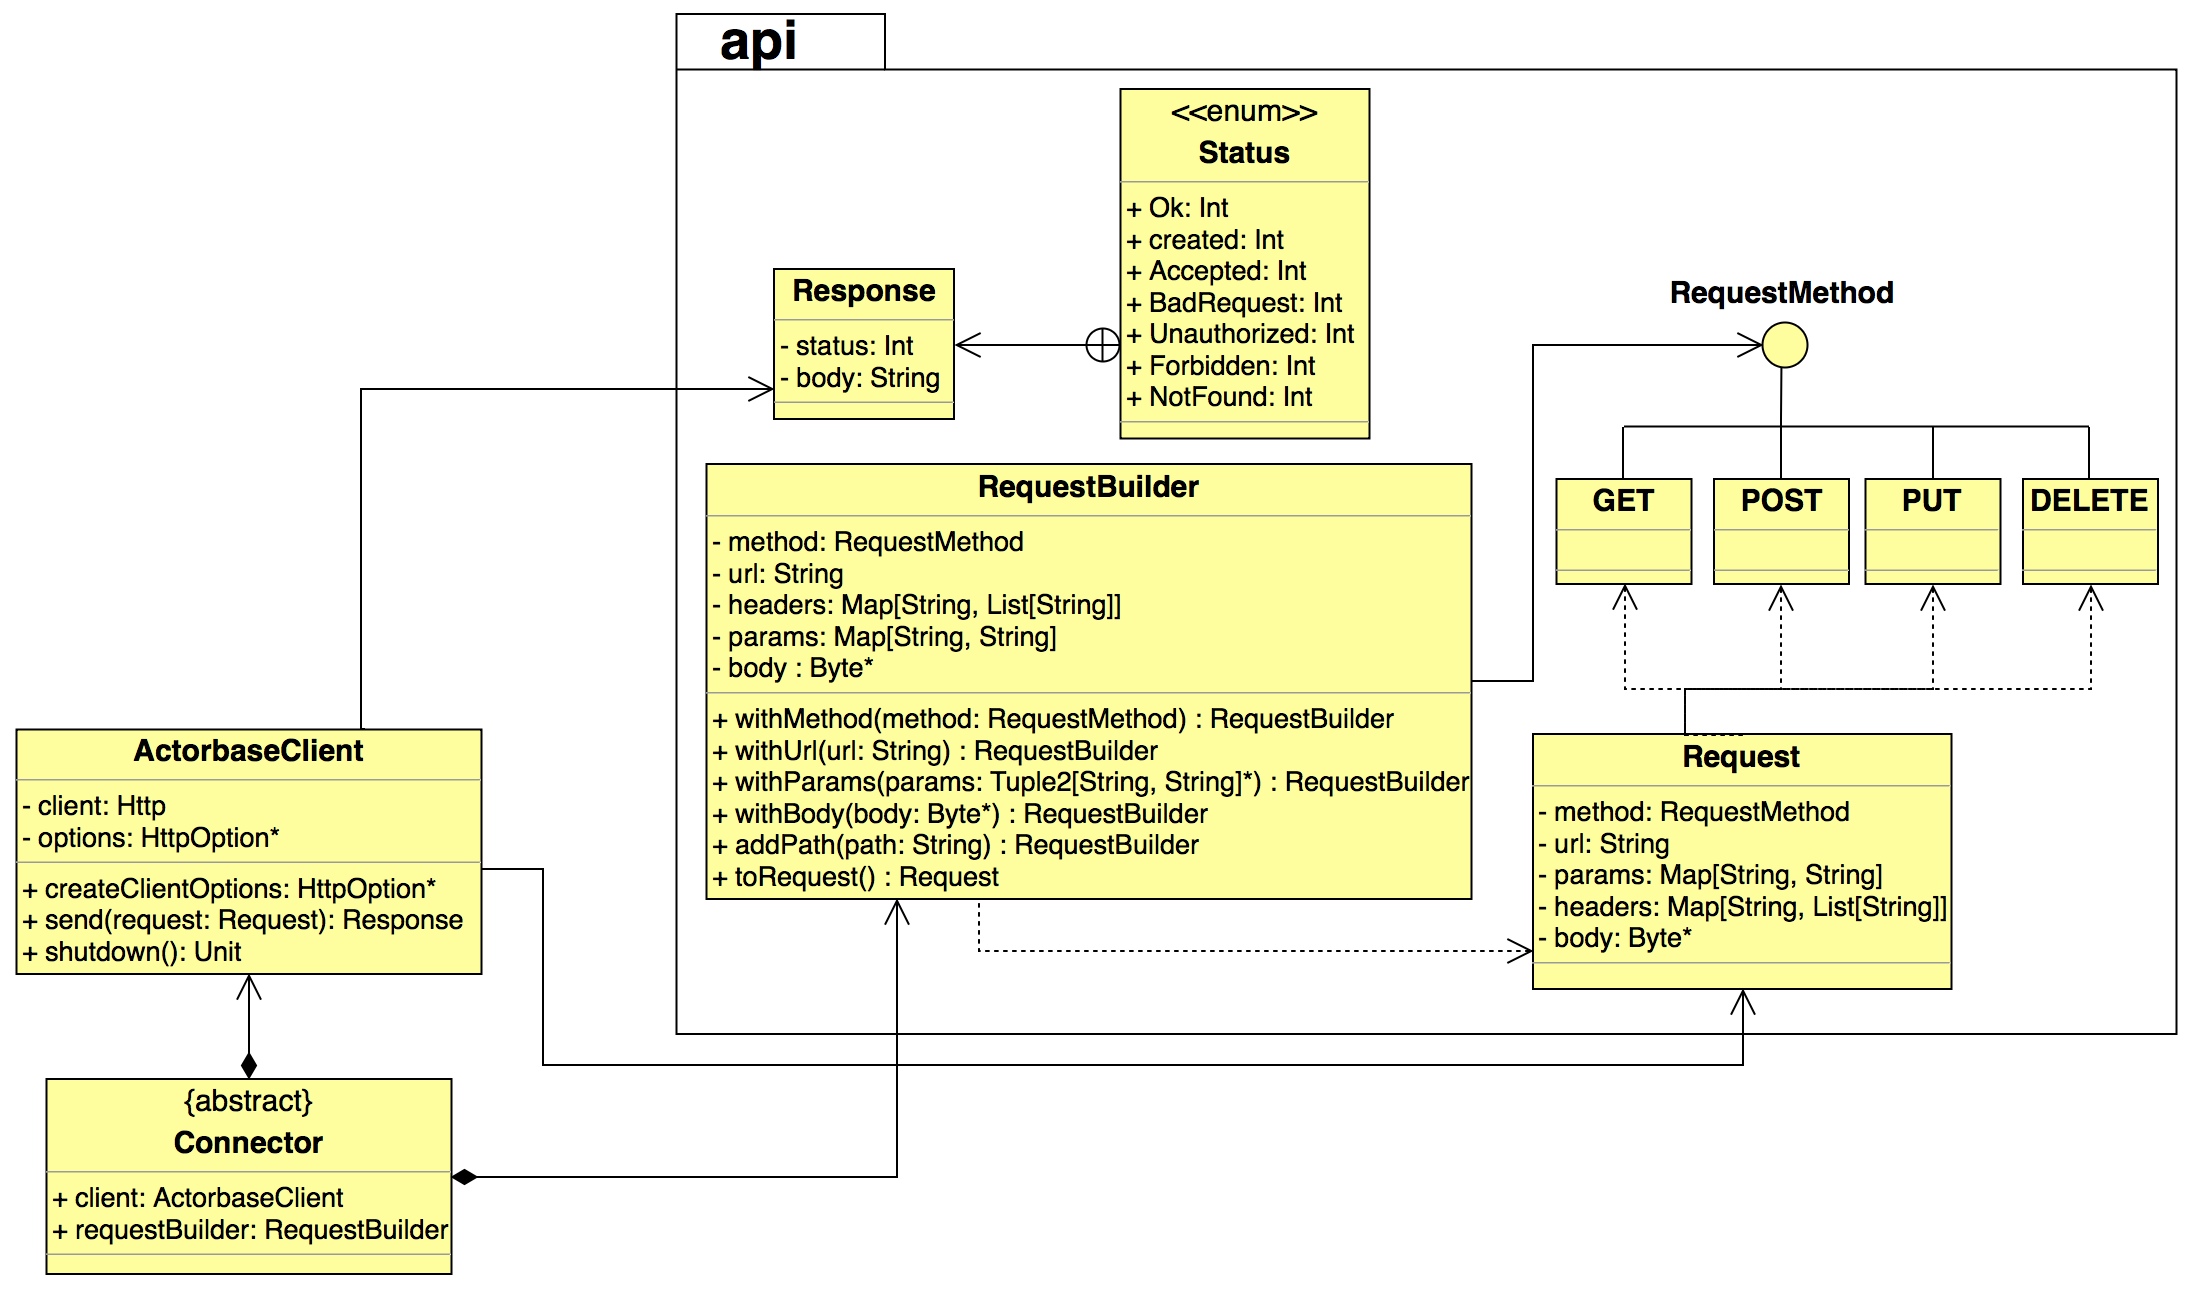
\includegraphics[width=0.9\textwidth,keepaspectratio]{RQ/Api.png}
    \caption{Driver: Package api}
  \end{center}
\end{figure}

\subsubsection{Descrizione}

\gloss{Package} che offre le strutture dati necessarie per la comunicazione con
il \gloss{server}, con la \gloss{cli} o eventuali programmi esterni. Si occupa
inoltre della gestione delle richieste \gloss{REST} da inviare utilizzando il
protocollo \gloss{HTTP}.

\subsubsection{Classi}

\paragraph{RequestMethod (abstract)}
\label{sec:actorbase::driver::client::api::RequestMethod}

\begin{figure}[H]
  \begin{center}
    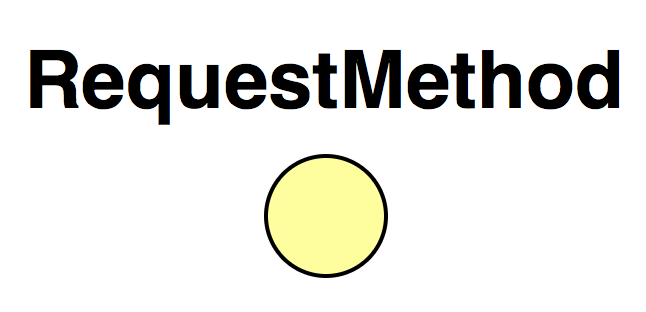
\includegraphics[width=0.9\textwidth,keepaspectratio]{RQ/RequestMethod.png}
    \caption{Driver: RequestMethod interface}
  \end{center}
\end{figure}

\subparagraph{Descrizione}

Classe astratta che rappresenta una generica richiesta \gloss{HTTP},
implementata utilizzando la specifica funzionalità \textit{case class} di Scala,
in modo da poter usufruirne mediante costrutti e algoritmi di \gloss{pattern
  matching}.

\subparagraph{Utilizzo}

Viene utilizzata come classe padre per l'implementazione delle richieste
\gloss{HTTP} da utilizzare nella comunicazione con il server.

\subparagraph{Ereditata da}

\begin{itemize}
\item \hyperref[sec:actorbase::driver::client::api::GET]{actorbase::driver::client::api::GET}
\item \hyperref[sec:actorbase::driver::client::api::POST]{actorbase::driver::client::api::POST}
\item \hyperref[sec:actorbase::driver::client::api::PUT]{actorbase::driver::client::api::PUT}
\item \hyperref[sec:actorbase::driver::client::api::DELETE]{actorbase::driver::client::api::DELETE}
\end{itemize}

% FINE REQUEST METHOD

\paragraph{GET (abstract)}
\label{sec:actorbase::driver::client::api::GET}

\begin{figure}[H]
  \begin{center}
    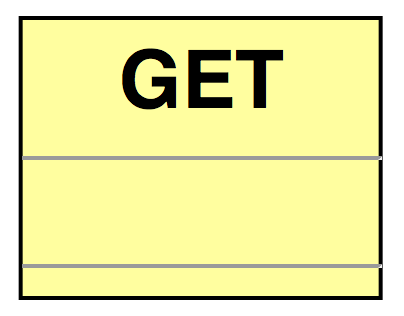
\includegraphics[width=0.9\textwidth,keepaspectratio]{RQ/Get.png}
    \caption{Driver: Oggetto rappresentante richiesta get}
  \end{center}
\end{figure}

\subparagraph{Descrizione}

Classe astratta che rappresenta una generica richiesta \gloss{HTTP} di tipo
\gloss{GET}, implementata utilizzando la specifica funzionalità \textit{case
  class} di Scala, in modo da poter usufruirne mediante costrutti e algoritmi di
\gloss{pattern matching}.

\subparagraph{Utilizzo}

Viene utilizzata come classe per l'implementazione delle richieste \gloss{HTTP}
di tipo \gloss{GET} da utilizzare nella comunicazione con il server.

\subparagraph{Eredita}

\begin{itemize}
\item \hyperref[sec:actorbase::driver::client::api::RequestMethod]{actorbase::driver::client::api::RequestMethod}
\end{itemize}

% FINE GET

\paragraph{POST (abstract)}
\label{sec:actorbase::driver::client::api::POST}

\begin{figure}[H]
  \begin{center}
    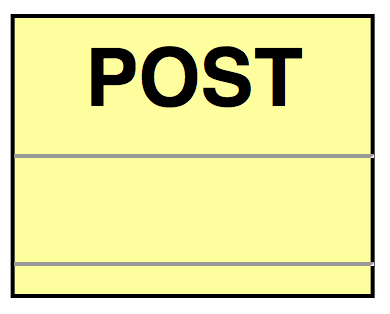
\includegraphics[width=0.9\textwidth,keepaspectratio]{RQ/Post.png}
    \caption{Driver: Oggetto rappresentante richiesta post}
  \end{center}
\end{figure}

\subparagraph{Descrizione}

Classe astratta che rappresenta una generica richiesta \gloss{HTTP} di tipo
\gloss{POST}, implementata utilizzando la specifica funzionalità \textit{case
  class} di Scala, in modo da poter usufruirne mediante costrutti e algoritmi di
\gloss{pattern matching}.

\subparagraph{Utilizzo}

Viene utilizzata come classe per l'implementazione delle richieste \gloss{HTTP}
di tipo \gloss{POST} da utilizzare nella comunicazione con il server.

\subparagraph{Eredita}

\begin{itemize}
\item \hyperref[sec:actorbase::driver::client::api::RequestMethod]{actorbase::driver::client::api::RequestMethod}
\end{itemize}

% FINE POST

\paragraph{PUT (abstract)}
\label{sec:actorbase::driver::client::api::PUT}

\begin{figure}[H]
  \begin{center}
    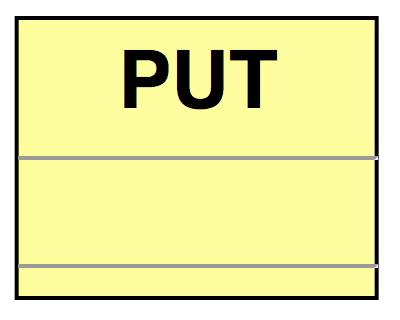
\includegraphics[width=0.9\textwidth,keepaspectratio]{RQ/Put.png}
    \caption{Driver: Oggetto rappresentante richiesta Put}
  \end{center}
\end{figure}

\subparagraph{Descrizione}

Classe astratta che rappresenta una generica richiesta \gloss{HTTP} di tipo
\gloss{PUT}, implementata utilizzando la specifica funzionalità \textit{case
  class} di Scala, in modo da poter usufruirne mediante costrutti e algoritmi di
\gloss{pattern matching}.

\subparagraph{Utilizzo}

Viene utilizzata come classe per l'implementazione delle richieste \gloss{HTTP}
di tipo \gloss{PUT} da utilizzare nella comunicazione con il server.

\subparagraph{Eredita}

\begin{itemize}
\item \hyperref[sec:actorbase::driver::client::api::RequestMethod]{actorbase::driver::client::api::RequestMethod}
\end{itemize}

% FINE PUT

\paragraph{DELETE (abstract)}
\label{sec:actorbase::driver::client::api::DELETE}

\begin{figure}[H]
  \begin{center}
    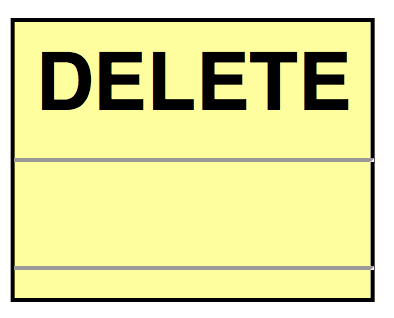
\includegraphics[width=0.9\textwidth,keepaspectratio]{RQ/Delete.png}
    \caption{Driver: Oggetto rappresentante richiesta Delete}
  \end{center}
\end{figure}

\subparagraph{Descrizione}

Classe astratta che rappresenta una generica richiesta \gloss{HTTP} di tipo
\gloss{DELETE}, implementata utilizzando la specifica funzionalità \textit{case
  class} di Scala, in modo da poter usufruirne mediante costrutti e algoritmi di
\gloss{pattern matching}.

\subparagraph{Utilizzo}

Viene utilizzata come classe per l'implementazione delle richieste \gloss{HTTP}
di tipo \gloss{DELETE} da utilizzare nella comunicazione con il server.

\subparagraph{Eredita}

\begin{itemize}
\item \hyperref[sec:actorbase::driver::client::api::RequestMethod]{actorbase::driver::client::api::RequestMethod}
\end{itemize}

% FINE DELETE

\paragraph{Request}
\label{sec:actorbase::driver::client::api::Request}

\begin{figure}[H]
  \begin{center}
    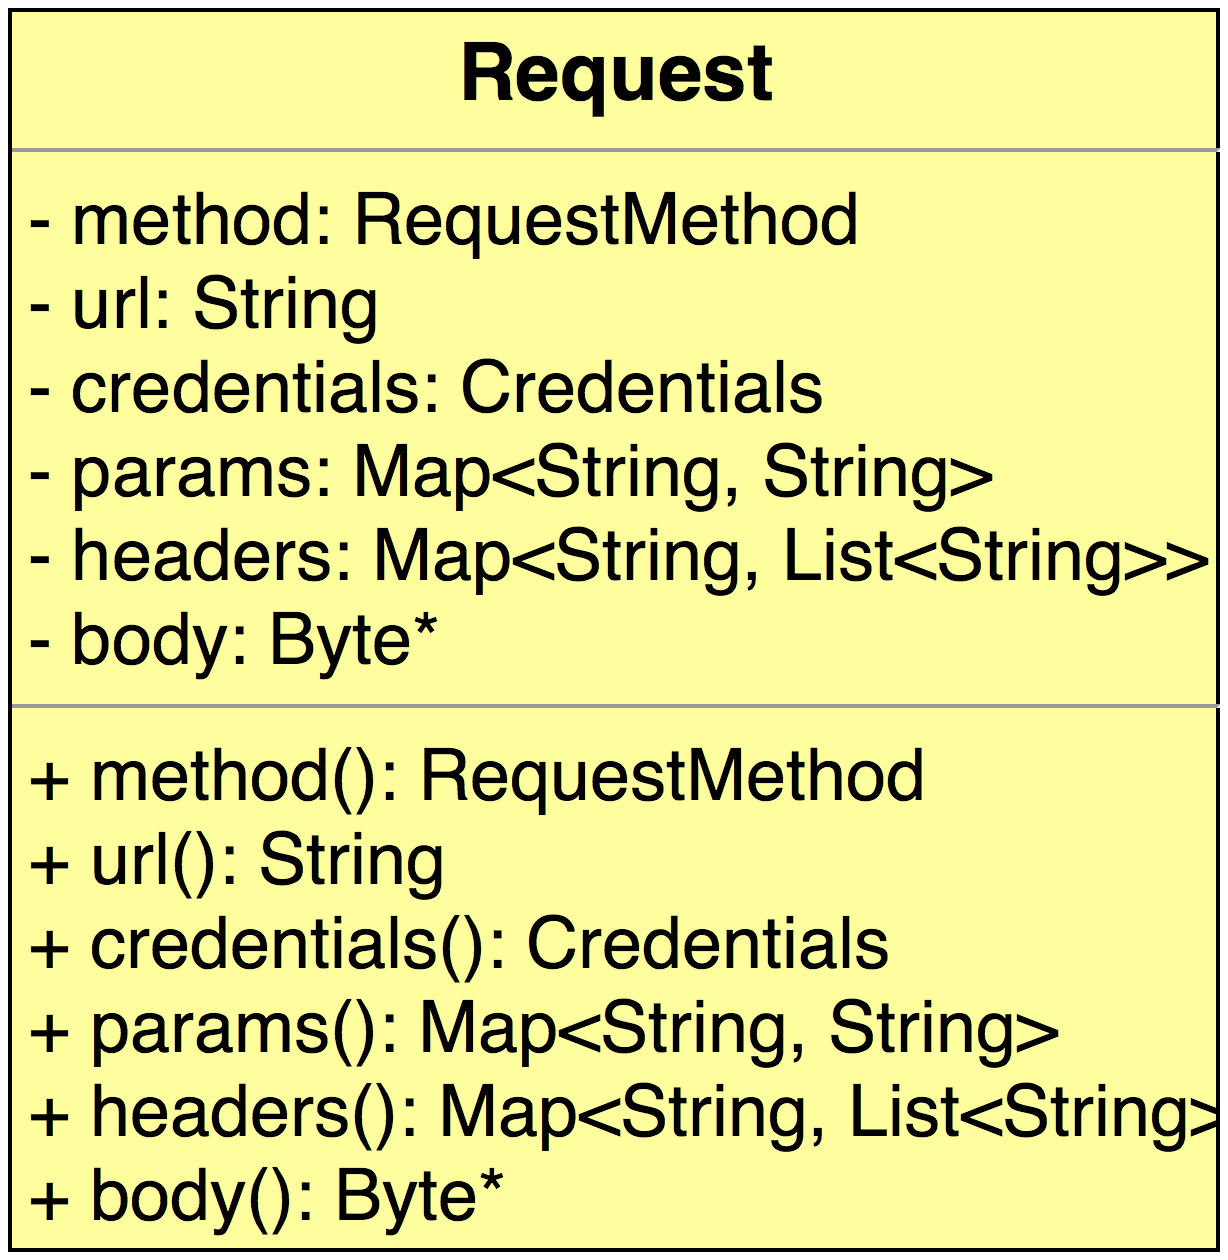
\includegraphics[width=0.9\textwidth,keepaspectratio]{RQ/Request.png}
    \caption{Driver: Classe request}
  \end{center}
\end{figure}

\subparagraph{Descrizione}

Classe che rappresenta una generica richiesta \gloss{HTTP}, implementata
utilizzando la specifica funzionalità \textit{case class} di Scala, in modo da
poter usufruirne mediante costrutti e algoritmi di \gloss{pattern matching},
racchiude al suo interno i parametri di richiesta, quali il metodo, di tipo
\hyperref[sec:actorbase::driver::client::api::RequestMethod]{RequestMethod},
l'\gloss{URL} a cui inviare la richiesta, gli \gloss{header} \gloss{HTTP}
associati, i parametri e il \gloss{payload}.

\subparagraph{Utilizzo}

Viene utilizzata come classe per l'implementazione delle richieste \gloss{HTTP}
di tipo \gloss{DELETE} da utilizzare nella comunicazione con il server. Viene
creata mediante il design pattern \gloss{Builder} nella classe
\hyperref[sec:actorbase::driver::client::api::RequestBuilder]{RequestBuilder}.

\subparagraph{Attributi}

\begin{tabular}{| p{2.5cm} | p{1.5cm} | p{2cm} | p{2.5cm} | p{8.5cm} |}
  \hline
  Nome & Accesso & Mutabilità & Tipo & Descrizione\\
  \hline
  method & private & immutabile & \hyperref[sec:actorbase::driver::api::RequestMethod]{RequestMethod} & Indica il tipo di richiesta \gloss{HTTP}\\
  \hline
  url & private & immutabile & String & Rappresenta l'indirizzo dell'\gloss{API} esposta sul server a cui inviare la richiesta\\
  \hline
  headers & private & immutabile & Map[String, List[String]] & Rappresenta gli \gloss{header} \gloss{HTTP} da associare alla richiesta\\
  \hline
  params & private & immutabile &  Map[String, String] & Rappresenta i parametri da allegare alla richiesta \gloss{HTTP}\\
  \hline
  body & private & immutabile & Array di Byte & Rappresenta i dati di \gloss{payload} da iniviare sul server\\
  \hline
\end{tabular}

% FINE REQUEST

\paragraph{Response}
\label{sec:actorbase::driver::client::api::Response}

\begin{figure}[H]
  \begin{center}
    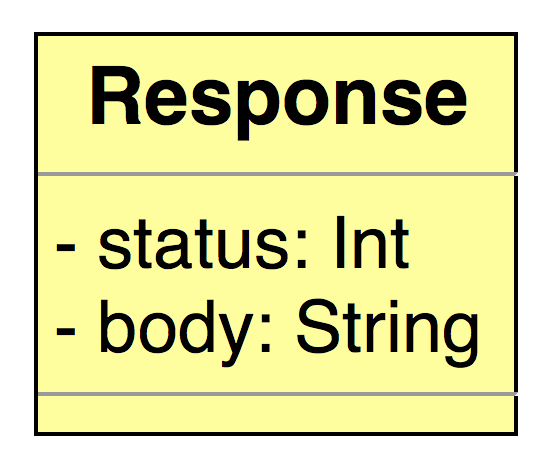
\includegraphics[width=0.9\textwidth,keepaspectratio]{RQ/Response.png}
    \caption{Driver: Classe response}
  \end{center}
\end{figure}

\subparagraph{Descrizione}

Classe che rappresenta una generica risposta \gloss{HTTP}, implementata
utilizzando la specifica funzionalità \textit{case class} di Scala, in modo da
poter usufruirne mediante costrutti e algoritmi di \gloss{pattern matching},
racchiude al suo interno i parametri di risposta, quali il codice di stato,
rappresentato da una enum interna
\hyperref[sec:actorbase::driver::client::api::Status]{Status} e il
\gloss{payload} di risposta in formato stringa.

\subparagraph{Utilizzo}

Viene utilizzata come classe per l'incapsulamento delle risposte \gloss{HTTP} da
utilizzare nella comunicazione con il server.

\subparagraph{Attributi}

\begin{tabular}{| p{3cm} | p{1.5cm} | p{2cm} | p{2cm} | p{8.5cm} |}
  \hline
  Nome & Accesso & Mutabilità & Tipo & Descrizione\\
  \hline
  status & private & immutabile & Int & Indica il codice di risposta \gloss{HTTP}\\
  \hline
  body & private & immutabile & String & Rappresenta i dati di \gloss{payload} ricevuti dal server\\
  \hline
\end{tabular}

% FINE RESPONSE

\paragraph{Status}
\label{sec:actorbase::driver::client::api::Status}

\subparagraph{Descrizione}

Enum interna a hyperref[sec:actorbase::driver::client::api::Response]{Response},
rappresenta il codice di ritorno della richiesta \gloss{HTTP} inviata al server.

\subparagraph{Utilizzo}

Viene utilizzata come classe per l'incapsulamento dei codici di ritorno
\gloss{HTTP} da utilizzare nella comunicazione con il server.

\subparagraph{Attributi}

\begin{tabular}{| p{3cm} | p{1.5cm} | p{2cm} | p{2cm} | p{8.5cm} |}
  \hline
  Nome & Accesso & Mutabilità & Tipo & Descrizione\\
  \hline
  OK & private & immutabile & Int & Indica il codice di risposta \gloss{HTTP} 200\\
  \hline
  Created & private & immutabile & Int & Indica il codice di risposta \gloss{HTTP} 201\\
  \hline
  Accepted & private & immutabile & Int & Indica il codice di risposta \gloss{HTTP} 202\\
  \hline
  BadRequest & private & immutabile & Int & Indica il codice di risposta \gloss{HTTP} 400\\
  \hline
  Unauthorized & private & immutabile & Int & Indica il codice di risposta \gloss{HTTP} 401\\
  \hline
  Forbidden & private & immutabile & Int & Indica il codice di risposta \gloss{HTTP} 403\\
  \hline
  NotFound & private & immutabile & Int & Indica il codice di risposta \gloss{HTTP} 404\\
  \hline
\end{tabular}

% FINE STATUS

\paragraph{RequestBuilder}
\label{sec:actorbase::driver::client::api::RequestBuilder}

\begin{figure}[H]
  \begin{center}
    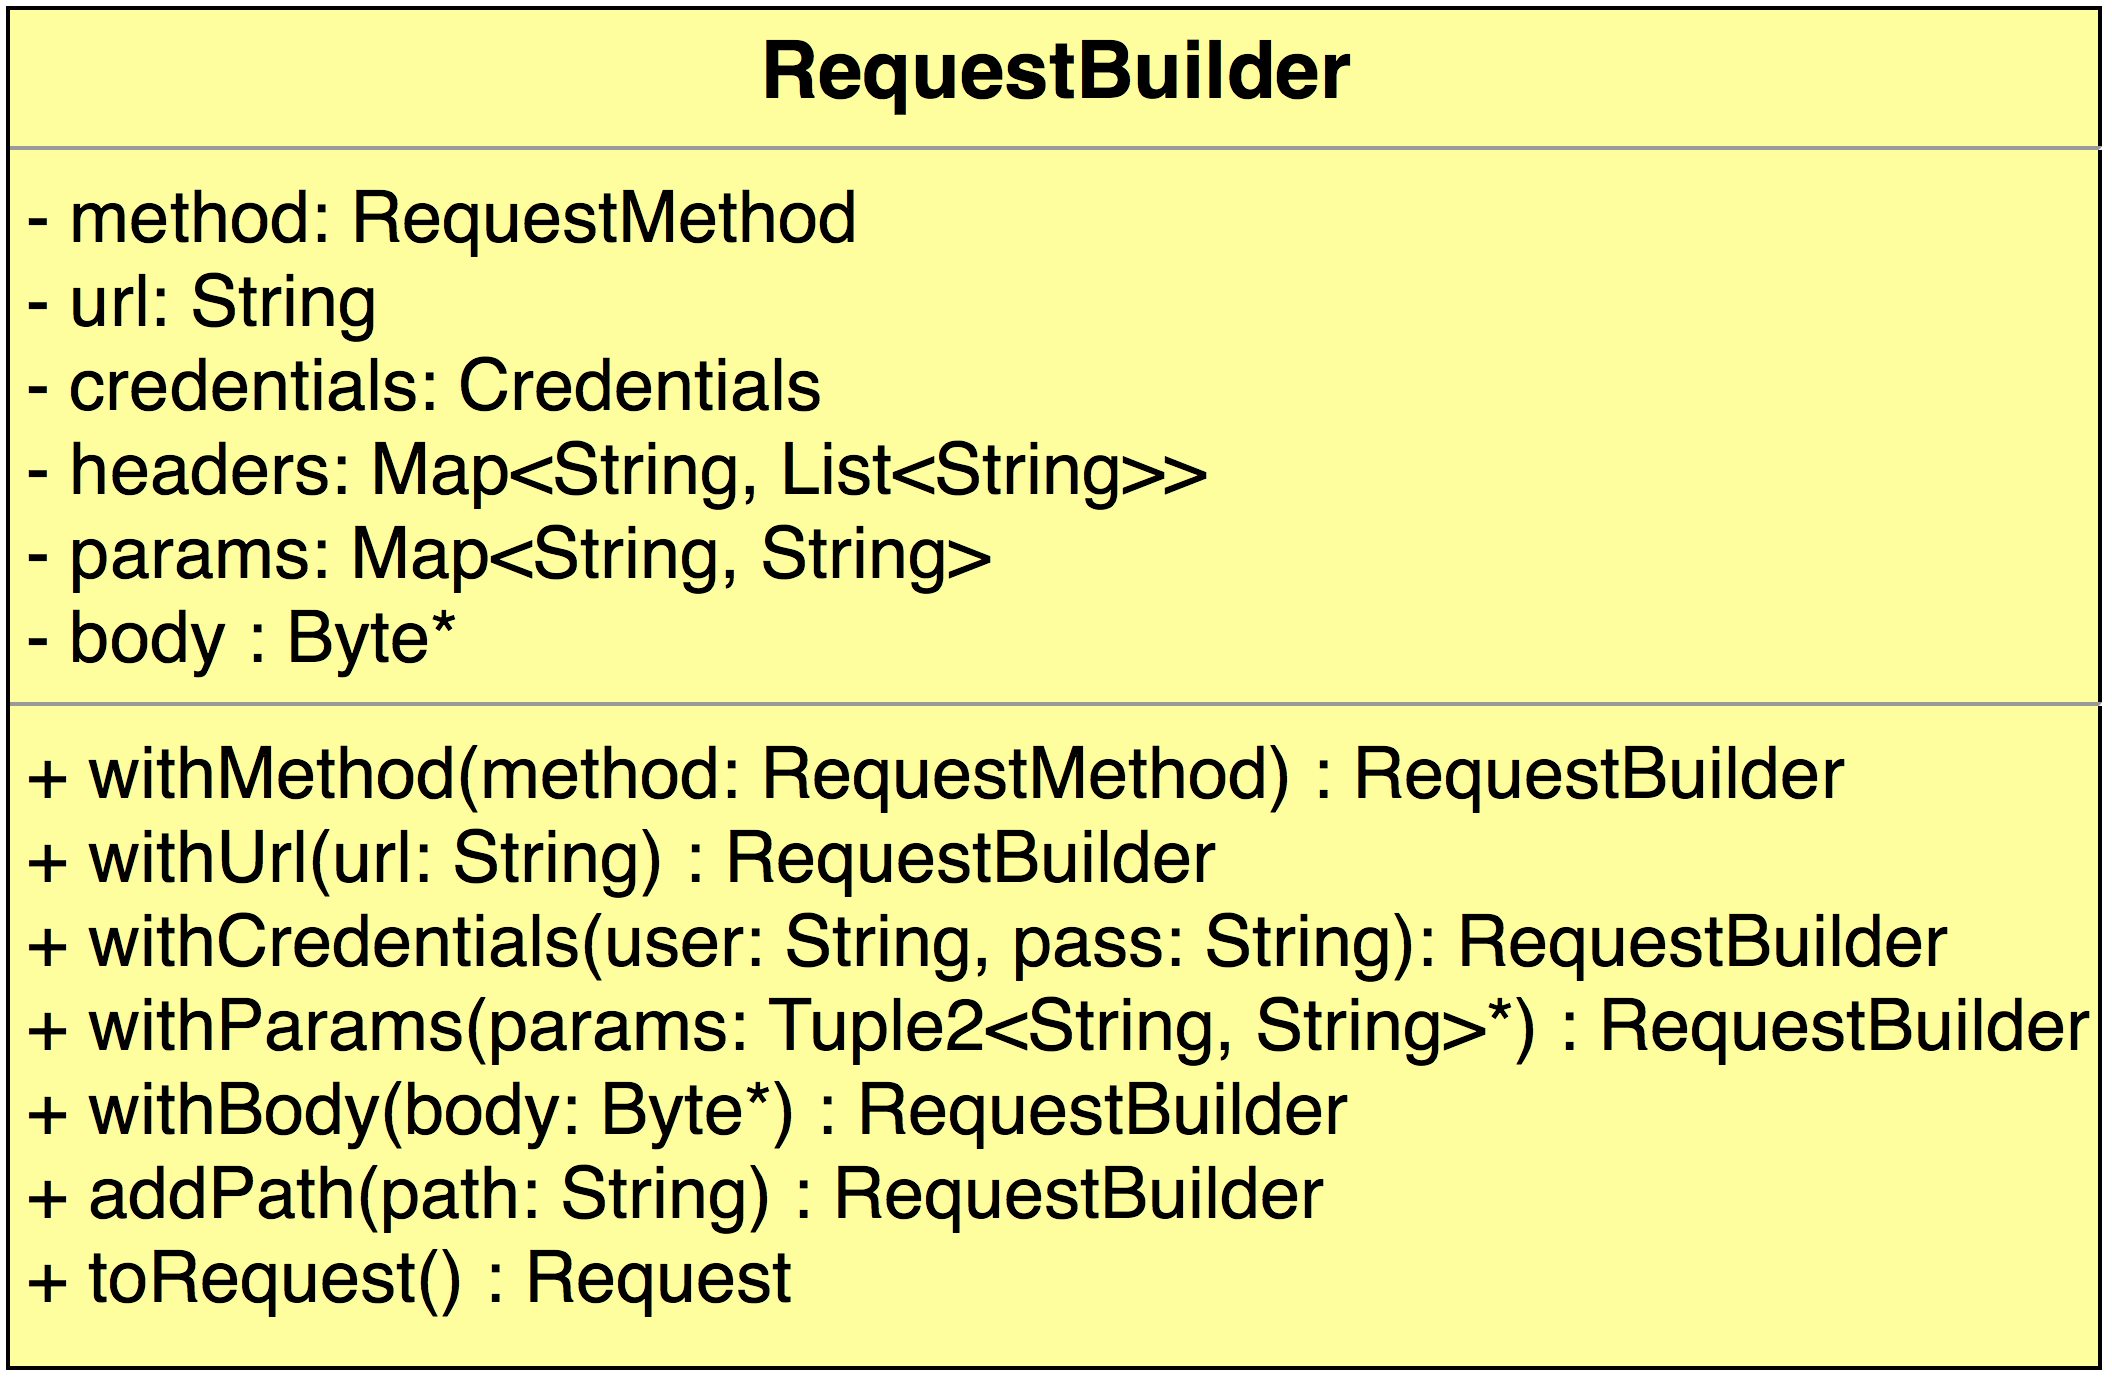
\includegraphics[width=0.9\textwidth,keepaspectratio]{RQ/RequestBuilder.png}
    \caption{Driver: Classe RequestBuilder}
  \end{center}
\end{figure}

\subparagraph{Descrizione}

Rappresenta una classe builder per la creazione di richieste \gloss{HTTP},
racchiude al suo interno i parametri di richiesta, quali il metodo, di tipo
\hyperref[sec:actorbase::driver::client::api::RequestMethod]{RequestMethod},
l'\gloss{URL} a cui inviare la richiesta, gli \gloss{header} \gloss{HTTP}
associati, i parametri e il \gloss{payload} e i metodi \verb=with= per
aggiungere attributi alla richiesta di tipo
\hyperref[sec:actorbase::driver::client::api::Request]{Request} da generare.

\subparagraph{Utilizzo}

Viene utilizzata come classe buider per la costruzione delle richieste
\gloss{HTTP} di tipo
\hyperref[sec:actorbase::driver::client::api::Request]{Request} da utilizzare
nella comunicazione con il server.

\subparagraph{Attributi}

\begin{tabular}{| p{2.5cm} | p{1.5cm} | p{2cm} | p{2.5cm} | p{8.5cm} |}
  \hline
  Nome & Accesso & Mutabilità & Tipo & Descrizione\\
  \hline
  method & private & immutabile & \hyperref[sec:actorbase::driver::api::RequestMethod]{RequestMethod} & Indica il tipo di richiesta \gloss{HTTP}\\
  \hline
  url & private & immutabile & String & Rappresenta l'indirizzo dell'\gloss{API} esposta sul server a cui inviare la richiesta\\
  \hline
  headers & private & immutabile & Map[String, List[String]] & Rappresenta gli \gloss{header} \gloss{HTTP} da associare alla richiesta\\
  \hline
  params & private & immutabile &  Map[String, String] & Rappresenta i parametri da allegare alla richiesta \gloss{HTTP}\\
  \hline
  body & private & immutabile & Array di Byte & Rappresenta i dati di \gloss{payload} da iniviare sul server\\
  \hline
\end{tabular}

\subparagraph{Metodi}

\begin{tabular}{| p{3cm} | p{1.5cm} | p{2.5cm} | p{10cm} |}
  \hline
  Nome & Accesso & Tipo di ritorno & Descrizione\\
  \hline
  withMethod & public & \hyperref[sec:actorbase::driver::client::api::RequestMethod]{RequestMethod} & Imposta il metodo di richiesta \gloss{HTTP}\\
  \hline
  withUrl & public & \hyperref[sec:actorbase::driver::client::api::RequestMethod]{RequestMethod} & Imposta l'indirizzo dell'\gloss{API} esposta sul server\\
  \hline
  withParams & public & \hyperref[sec:actorbase::driver::client::api::RequestMethod]{RequestMethod} & Imposta i parametri da inviare allegati alla richiesta \gloss{HTTP}\\
  \hline
  withBody & public & \hyperref[sec:actorbase::driver::client::api::RequestMethod]{RequestMethod} & Imposta il \gloss{payload} da inviare allegato alla richiesta \gloss{HTTP}\\
  \hline
  addPath & public & \hyperref[sec:actorbase::driver::client::api::RequestMethod]{RequestMethod} & Aggiunge eventuali indirizzi aggiuntivi all'\gloss{url} della richiesta \gloss{HTTP}\\
  \hline
  toRequest & public & \hyperref[sec:actorbase::driver::client::api::Request]{Request} & Trasforma l'oggetto riferito da \gloss{this}, in un oggetto di tipo \hyperref[sec:actorbase::driver::client::api::Request]{Request}\\
  \hline
\end{tabular}

\subparagraph{Parametri}

\begin{center}
  \textbf{withMethod}
\end{center}
\begin{tabular}{| p{3cm} | p{3.5cm} | p{8.5cm} |}
  \hline
  Nome & Tipo & Descrizione\\
  \hline
  method & \hyperref[actorbase::driver::client::api::RequestMethod]{RequestMethod} & Rappresenta il tipo di richiesta \gloss{HTTP} da inviare al server\\
  \hline
\end{tabular}

\begin{center}
  \textbf{withUrl}
\end{center}
\begin{tabular}{| p{3cm} | p{3.5cm} | p{8.5cm} |}
  \hline
  Nome & Tipo & Descrizione\\
  \hline
  url & String & Rappresenta il la \gloss{route} dell'\gloss{API} esposta sul server a cui inviare le richieste\\
  \hline
\end{tabular}

\begin{center}
  \textbf{withParams}
\end{center}
\begin{tabular}{| p{3cm} | p{3.5cm} | p{8.5cm} |}
  \hline
  Nome & Tipo & Descrizione\\
  \hline
  params & array di Tuple2[String, String] & Rappresenta i parametri da allegare alle richieste \gloss{HTTP}\\
  \hline
\end{tabular}

\begin{center}
  \textbf{withBody}
\end{center}
\begin{tabular}{| p{3cm} | p{3.5cm} | p{8.5cm} |}
  \hline
  Nome & Tipo & Descrizione\\
  \hline
  body & array di Byte & Rappresenta il \gloss{payload} da allegare alle richieste \gloss{HTTP}\\
  \hline
\end{tabular}

\begin{center}
  \textbf{addPath}
\end{center}
\begin{tabular}{| p{3cm} | p{3.5cm} | p{8.5cm} |}
  \hline
  Nome & Tipo & Descrizione\\
  \hline
  path & String & Rappresenta l'eventuale indirizzo parziale da aggiungere all'\gloss{url} da allegare alle richieste \gloss{HTTP}\\
  \hline
\end{tabular}

% SONO QUI 04/05 6:07 P.M.

\subsection{actorbase::driver::data}
\label{sec:actorbase::driver::data}

\begin{figure}[H]
  \begin{center}
    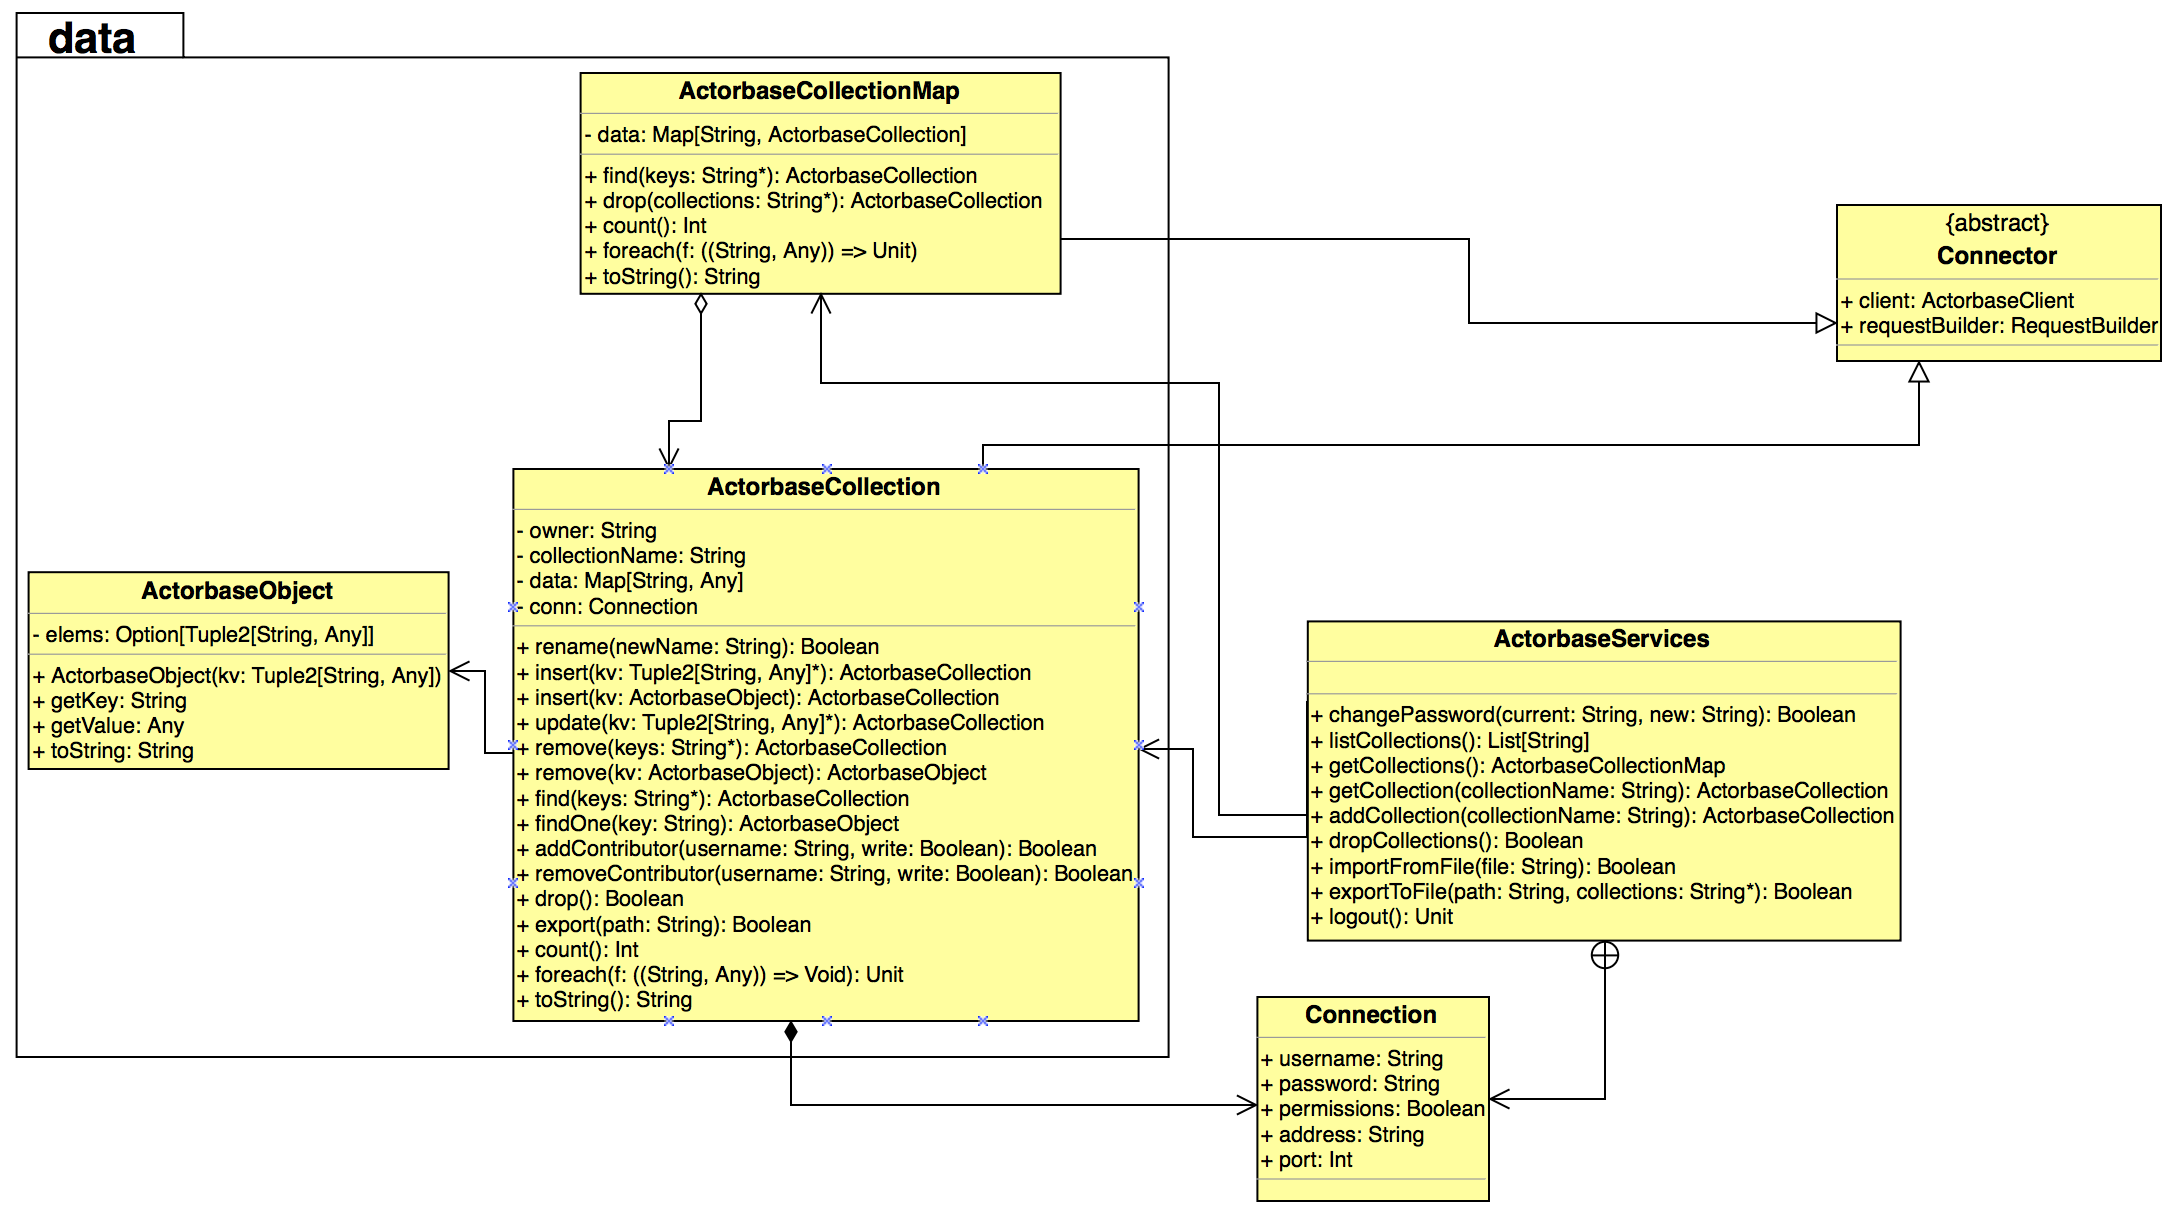
\includegraphics[width=0.9\textwidth,keepaspectratio]{RQ/Data.png}
    \caption{Driver: Package data}
  \end{center}
\end{figure}

\subsubsection{Descrizione}

\gloss{Package} che offre le strutture dati utili alla gestione dei contenuti
della base di dati in locale, permettendo di eseguire le comuni operazioni di
\gloss{CRUD} e ricerche più accurate in maniera semplificata, riflettendo le
eventuali modifiche locali sul server remoto che contiene i dati originali.

\subsubsection{Classi}

\paragraph{ActorbaseObject}
\label{sec:actorbase::driver::data::ActorbaseObject}

\begin{figure}[H]
  \begin{center}
    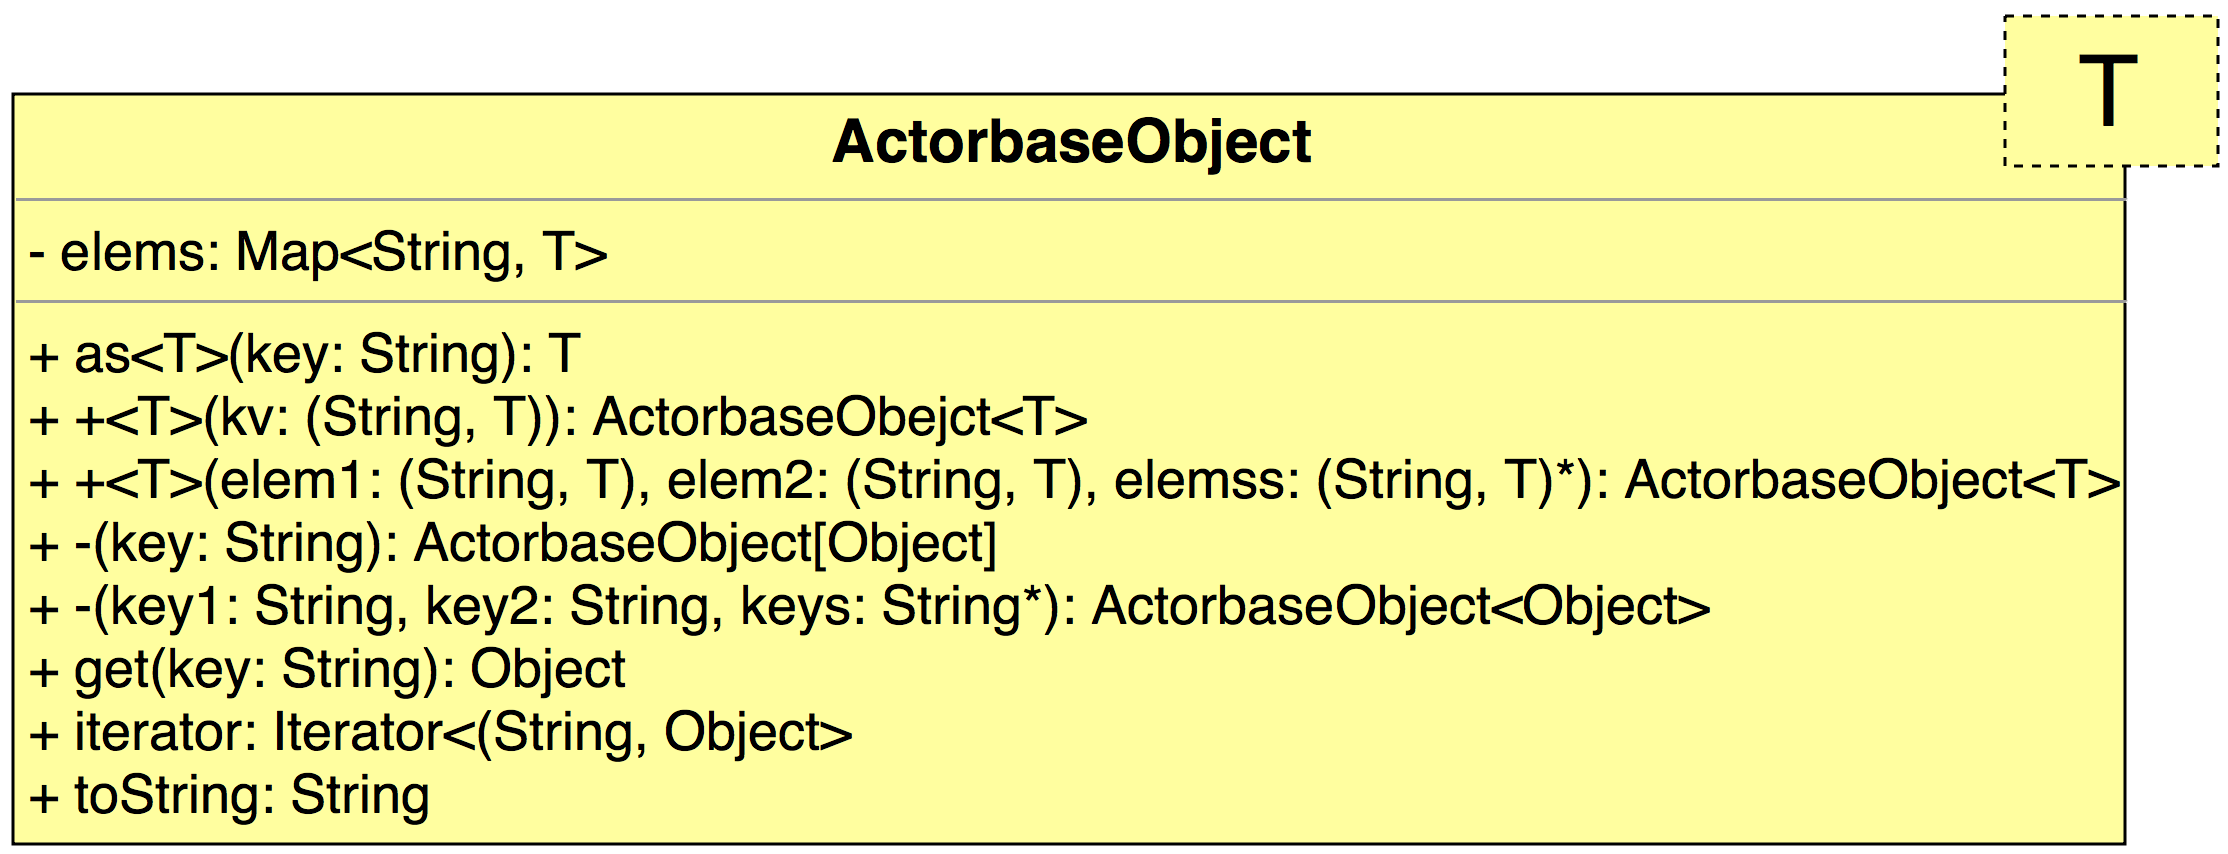
\includegraphics[width=0.9\textwidth,keepaspectratio]{RQ/ActorbaseObject.png}
    \caption{Driver: Classe ActorbaseObject}
  \end{center}
\end{figure}

\subparagraph{Descrizione}

Interfaccia che rappresenta un oggetto generico contenente una coppia
chiave-valore ricevuto dal \gloss{server}.

\subparagraph{Utilizzo}

Classe utilizzata per agevolare le ricerche specifiche all'interno delle
\gloss{collezioni} del \gloss{database}.

\subparagraph{Attributi}

\begin{tabular}{| p{1.5cm} | p{1.5cm} | p{2cm} | p{3.5cm} | p{8.5cm} |}
  \hline
  Nome & Accesso & Mutabilità & Tipo & Descrizione\\
  \hline
  elems & private & immutabile & \gloss{Option[Tuple2[String, Any]]} & Generica coppia chiave-valore, rappresenta un oggetto del \gloss{database}\\
  \hline
\end{tabular}

\subparagraph{Metodi}

\begin{tabular}{| p{3cm} | p{1.5cm} | p{2.5cm} | p{10cm} |}
  \hline
  Nome & Accesso & Tipo di ritorno & Descrizione\\
  \hline
  ActorbaseObject & public & \gloss{Tuple2[String, Any]}  & Costruttore dell'oggetto ActorbaseObject\\
  \hline
  getKey & public & String & Ritorna l'attributo chiave di tipo String\\
  \hline
  getValue & public & \gloss{Any} & Ritorna l'attributo valore di tipo \gloss{Any}\\
  \hline
  toString & public & String & Ritorna l'oggetto di tipo ActorbaseObject in formato String\\
  \hline
\end{tabular}

\subparagraph{Parametri}

\begin{center}
  \textbf{ActorbaseObject}
\end{center}
\begin{tabular}{| p{3cm} | p{3.5cm} | p{8.5cm} |}
  \hline
  Nome & Tipo & Descrizione\\
  \hline
  kv & \gloss{Tuple2[String, Any]} & Coppia chiave-valore, rappresenta un generico oggetto del \gloss{database}\\
  \hline
\end{tabular}

% FINE ACTORBASEOBJECT

\paragraph{actorbase::driver::data::ActorbaseCollection}
\label{sec:actorbase::driver::data::ActorbaseCollection}

\begin{figure}[H]
  \begin{center}
    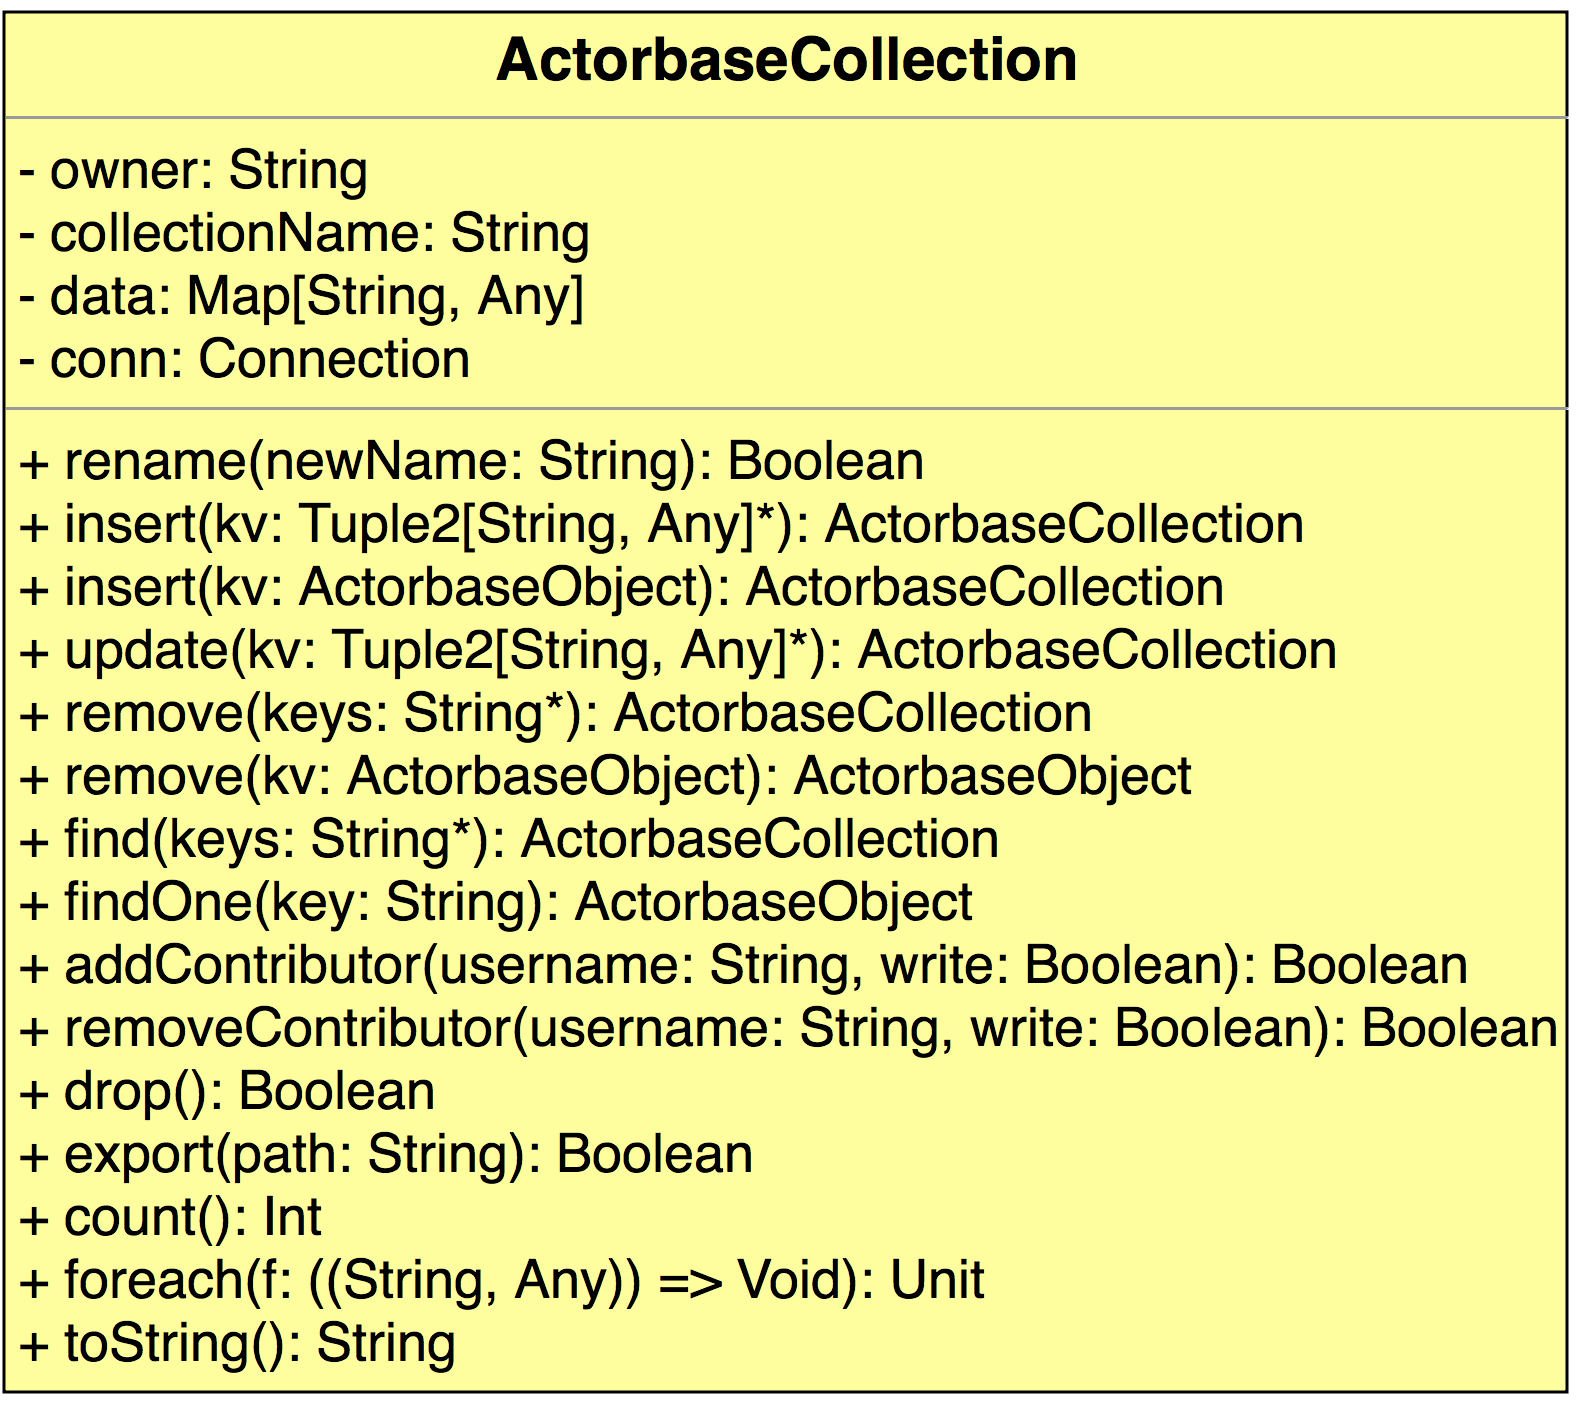
\includegraphics[width=0.9\textwidth,keepaspectratio]{RQ/ActorbaseCollection.png}
    \caption{Driver: Classe ActorbaseCollection}
  \end{center}
\end{figure}

\subparagraph{Descrizione}

Classe che rappresenta una singola \gloss{collezione} del \gloss{database}.

\subparagraph{Utilizzo}

Questa classe viene utilizzata per la rappresentazione di una singola
\gloss{collezione} vista come insieme di oggetti di tipo coppia chiave-valore.
Il valore può essere qualsiasi tipo, inclusi oggetti arbitrari creati
all'interno di un programma \gloss{Scala}. Offre metodi di utilità e
navigabilità dei contenuti.

\subparagraph{Eredita}

\begin{itemize}
\item \hyperref[sec:actorbase::driver::client::Connector]{actorbase::driver::client::Connector}.
\end{itemize}

\subparagraph{Attributi}

\begin{tabular}{| p{2.5cm} | p{1.5cm} | p{2cm} | p{2.5cm} | p{8.5cm} |}
  \hline
  Nome & Accesso & Mutabilità & Tipo & Descrizione\\
  \hline
  owner & private & immutabile & String & Creatore della \gloss{collezione}\\
  \hline
  collectionName & private & immutabile & String & Nome della \gloss{collezione}\\
  \hline
  data & private & immutabile & Map[String, Any] & Mappa contenente le coppie chiave-valore della \gloss{collezione}\\
  \hline
  conn & private & immutabile & \hyperref[sec:actorbase::driver::Connection]{Connection} & Oggetto che rappresenta i parametri di connessione al \gloss{server}\\
  \hline
\end{tabular}

\subparagraph{Metodi}

% TODO: Da completare

\begin{tabular}{| p{3cm} | p{1.5cm} | p{2.5cm} | p{10cm} |}
  \hline
  Nome & Accesso & Tipo di ritorno & Descrizione\\
  \hline
  insert & public & \hyperref[sec::actorbase::driver::data::ActorbaseCollection]{ActorbaseColletion} & Inserisce una o più coppie chiave-valore all'interno di Actorbase\\
  \hline
  insert & public & \hyperref[sec::actorbase::driver::data::ActorbaseCollection]{ActorbaseColletion} & Inserisce un'oggetto di tipo \hyperref[sec:actorbase::driver::data::ActorbaseObject]{ActorbaseObject}\\
  \hline
  update & public & \hyperref[sec::actorbase::driver::data::ActorbaseCollection]{ActorbaseColletion} & Aggiorna la coppia chiave-valore all'interno della \gloss{collezione}\\
  \hline
  remove & public & \hyperref[sec:actorbase::driver::data::ActorbaseCollection]{ActorbaseCollection} & Rimuove una o più coppie chiave-valore dal sistema\\
  \hline
  remove & public & \hyperref[sec:actorbase::driver::data::ActorbaseObject]{ActorbaseObject} & Rimuove una coppia chiave-valore dal sistema\\
  \hline
  find & public & \hyperref[sec:actorbase::driver::data::ActorbaseCollection]{ActorbaseCollection} & Cerca uno o più coppie-chiave valore nel sistema\\
  \hline
  findOne & public & \hyperref[sec:actorbase::driver::data::ActorbaseObject]{ActorbaseObject} & Cerca una coppia chiave-valore nel sistema\\
  \hline
  addContributor & public & Boolean & Aggiunge un \gloss{collaboratore} alla \gloss{collezione}\\
  \hline
  removeContributor & public & Boolean & Rimuove un \gloss{collaborator} dalla \gloss{collezione}\\
  \hline
  drop & public & Boolean & Cancella la \gloss{collezione}\\
  \hline
  count & public & Int & Conta il numero di coppie chiave-valore che formano la \gloss{collezione}\\
  \hline
  foreach & public & Unit & Permette di visitare l'intera \gloss{collezione} applicando una funzione ad ogni \gloss{item}\\
  \hline
  toString & public & String & Ritorna la \gloss{collezione} in formato String \gloss{JSON}\\
  \hline
\end{tabular}

\subparagraph{Parametri}

% TODO: Da completare

\begin{center}
  \textbf{insert}
\end{center}
\begin{tabular}{| p{3cm} | p{3.5cm} | p{8.5cm} |}
  \hline
  Nome & Tipo & Descrizione\\
  \hline
  kv & \gloss{vararg} di Tuple2[String, Any] & Rappresenta una sequenza di Tuple2[String, Any] da inserire nella \gloss{collezione}\\
  \hline
\end{tabular}

\begin{center}
  \textbf{insert (overload)}
\end{center}
\begin{tabular}{| p{3cm} | p{3.5cm} | p{8.5cm} |}
  \hline
  Nome & Tipo & Descrizione\\
  \hline
  kv & \hyperref[sec:actorbase::driver::data::ActorbaseObject]{ActorbaseObject} & Rappresenta un oggetto del sistema Actorbase da inserire nel sistema\\
  \hline
\end{tabular}

\begin{center}
  \textbf{update}
\end{center}
\begin{tabular}{| p{3cm} | p{3.5cm} | p{8.5cm} |}
  \hline
  Nome & Tipo & Descrizione\\
  \hline
  kv & \gloss{vararg} di Tuple2[String, Any] & Rappresenta una sequenza di Tuple2[String, Any] da aggiornare nella \gloss{collezione}\\
  \hline
\end{tabular}

\begin{center}
  \textbf{remove}
\end{center}
\begin{tabular}{| p{3cm} | p{3.5cm} | p{8.5cm} |}
  \hline
  Nome & Tipo & Descrizione\\
  \hline
  keys & \gloss{vararg} di String & Rappresenta una sequenza di String, rappresentano le chiavi da rimuovere dal sistema\\
  \hline
\end{tabular}

\begin{center}
  \textbf{remove (overload)}
\end{center}
\begin{tabular}{| p{3cm} | p{3.5cm} | p{8.5cm} |}
  \hline
  Nome & Tipo & Descrizione\\
  \hline
  kv & \hyperref[sec:actorbase::driver::data::ActorbaseObject]{ActorbaseObject} & Rappresenta un oggetto di tipo chiave-valore del sistema, rappresentano le chiavi da rimuovere dal sistema\\
  \hline
\end{tabular}

\begin{center}
  \textbf{find}
\end{center}
\begin{tabular}{| p{3cm} | p{3.5cm} | p{8.5cm} |}
  \hline
  Nome & Tipo & Descrizione\\
  \hline
  keys & \gloss{vararg} di String & Rappresenta una sequenza di String, sono chiavi da ricercare nel sistema\\
  \hline
\end{tabular}

\begin{center}
  \textbf{findOne}
\end{center}
\begin{tabular}{| p{3cm} | p{3.5cm} | p{8.5cm} |}
  \hline
  Nome & Tipo & Descrizione\\
  \hline
  key & String & Rappresenta una String da ricercare nel sistema \\
  \hline
\end{tabular}

\begin{center}
  \textbf{addContributor}
\end{center}
\begin{tabular}{| p{3cm} | p{3.5cm} | p{8.5cm} |}
  \hline
  Nome & Tipo & Descrizione\\
  \hline
  username & String & Rappresenta lo \gloss{username} dell'utente da aggiungere ai collaboratori della \gloss{collezione}\\
  \hline
\end{tabular}

\begin{center}
  \textbf{removeContributor}
\end{center}
\begin{tabular}{| p{3cm} | p{3.5cm} | p{8.5cm} |}
  \hline
  Nome & Tipo & Descrizione\\
  \hline
  username & String & Rappresenta lo \gloss{username} dell'utente da rimuove ai collaboratori della \gloss{collezione}\\
  \hline
\end{tabular}

\begin{center}
  \textbf{foreach}
\end{center}
\begin{tabular}{| p{3cm} | p{3.5cm} | p{8.5cm} |}
  \hline
  Nome & Tipo & Descrizione\\
  \hline
  f: ((A, B)) => Unit  & Funzione anonima & Rappresenta la funzione da applicare a tutti gli \gloss{item} della \gloss{collezione}\\
  \hline
\end{tabular}

% TODO ACTORBASECOLLECTION

\paragraph{actorbase::driver::data::ActorbaseCollectionMap}
\label{sec:actorbase::driver::data::ActorbaseCollectionMap}

\begin{figure}[H]
  \begin{center}
    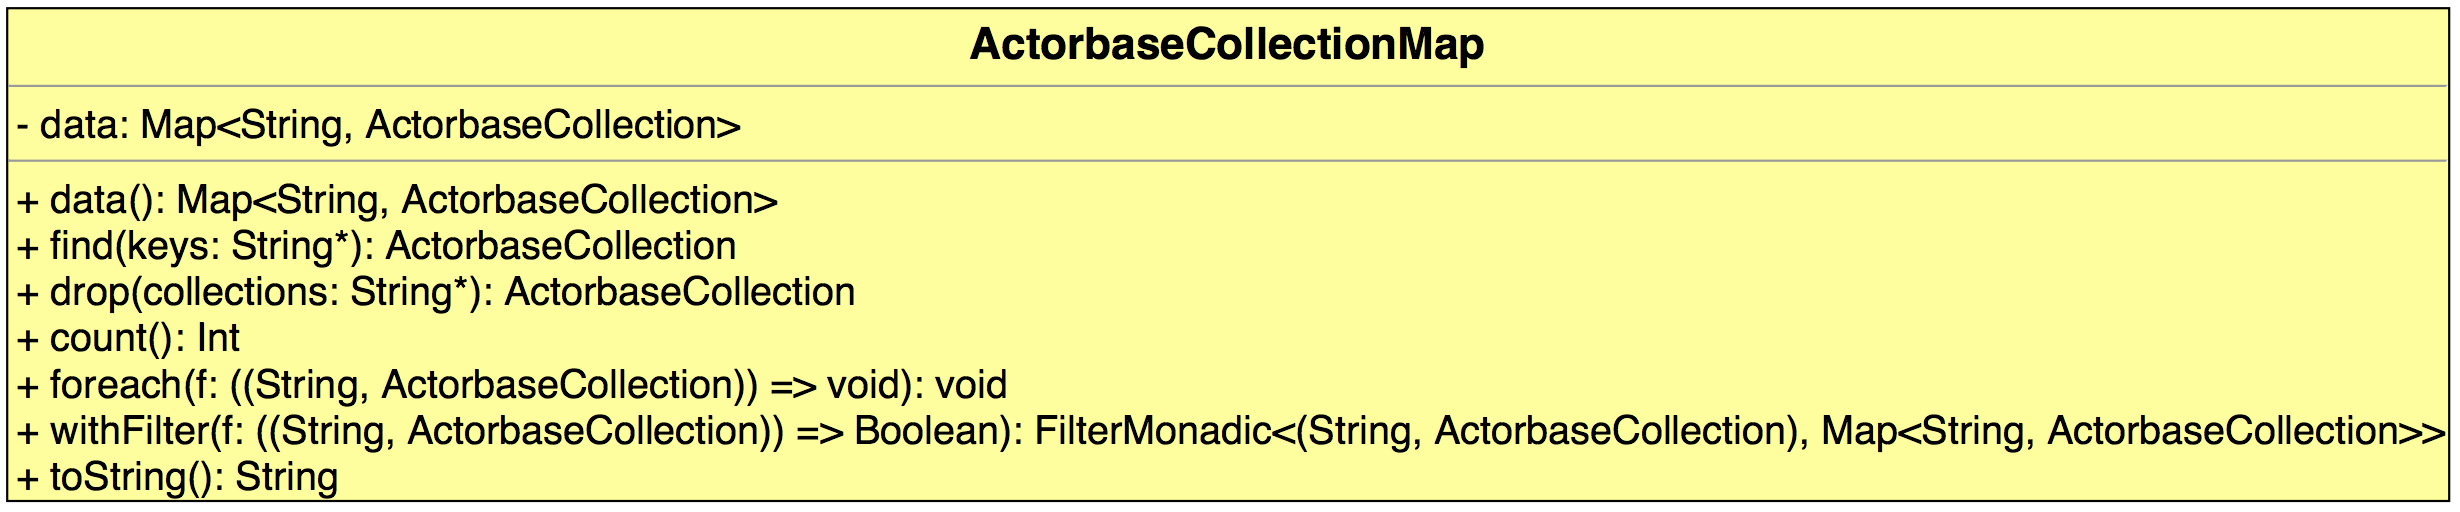
\includegraphics[width=0.9\textwidth,keepaspectratio]{RQ/ActorbaseCollectionMap.png}
    \caption{Driver: Classe ActorbaseCollectionMap}
  \end{center}
\end{figure}

\subparagraph{Descrizione}

Classe che rappresenta una \gloss{collezione} di \gloss{collezione} del sistema.

\subparagraph{Utilizzo}

Questa classe viene utilizzata per la rappresentazione dell'aggregazione di
\gloss{collezioni}, è formata da una mappa di coppie nomecollezione -
\hyperref[sec:actorbase::driver::data::ActorbaseCollection]{ActorbaseCollection}.

\subparagraph{Eredita}

\begin{itemize}
\item \hyperref[sec:actorbase::driver::client::Connector]{actorbase::driver::client::Connector}.
\end{itemize}

\subparagraph{Attributi}

\begin{tabular}{| p{2.5cm} | p{1.5cm} | p{2cm} | p{2.5cm} | p{8.5cm} |}
  \hline
  Nome & Accesso & Mutabilità & Tipo & Descrizione\\
  \hline
  data & private & mutabile & TreeMap[String, \hyperref[sec:actorbase::driver::data::ActorbaseCollection]{ActorbaseCollection}] & Mappa che rappresenta un insieme di \hyperref[sec:actorbase::driver::data::ActorbaseCollection]{ActorbaseCollection}\\
  \hline
\end{tabular}

\subparagraph{Metodi}

% TODO: Da completare

\begin{tabular}{| p{3cm} | p{1.5cm} | p{2.5cm} | p{10cm} |}
  \hline
  Nome & Accesso & Tipo di ritorno & Descrizione\\
  \hline
  find & public & \hyperref[sec:actorbase::driver::data::ActorbaseCollection]{ActorbaseCollect\allowbreak{}ion} & Cerca uno o più coppie-chiave valore nelle \gloss{collezioni}\\
  \hline
  drop & public & Boolean & Cancella una o più \gloss{collezione}\\
  \hline
  foreach & public & Unit & Permette di visitare l'intera \gloss{collezione} di \gloss{collezioni} applicando una funzione ad ogni \gloss{item}\\
  \hline
  toString & public & String & Ritorna la \gloss{collezione} in formato Stringa \gloss{JSON}\\
  \hline
\end{tabular}

\subparagraph{Parametri}

% TODO: Da completare

\begin{center}
  \textbf{find}
\end{center}
\begin{tabular}{| p{3cm} | p{3.5cm} | p{8.5cm} |}
  \hline
  Nome & Tipo & Descrizione\\
  \hline
  keys & \gloss{vararg} di String & Rappresenta una sequenza di String, sono chiavi da ricercare nella \gloss{collezione}\\
  \hline
\end{tabular}

\begin{center}
  \textbf{drop}
\end{center}
\begin{tabular}{| p{3cm} | p{3.5cm} | p{8.5cm} |}
  \hline
  Nome & Tipo & Descrizione\\
  \hline
  collections & \gloss{vararg} di String & Rappresenta una sequenza di String, sono nomi di \gloss{collezioni} da rimuovere\\
  \hline
\end{tabular}

\begin{center}
  \textbf{foreach}
\end{center}
\begin{tabular}{| p{3cm} | p{3.5cm} | p{8.5cm} |}
  \hline
  Nome & Tipo & Descrizione\\
  \hline
  f: ((A, B)) => Unit  & Funzione anonima & Rappresenta la funzione da applicare a tutti gli \gloss{item} della \gloss{collezione}\\
  \hline
\end{tabular}

% FINITO ACTORBASECOLLECTIONMAP

\subsection{actorbase::driver::exceptions}
\label{sec:actorbase::driver::exceptions}

\begin{figure}[H]
  \begin{center}
    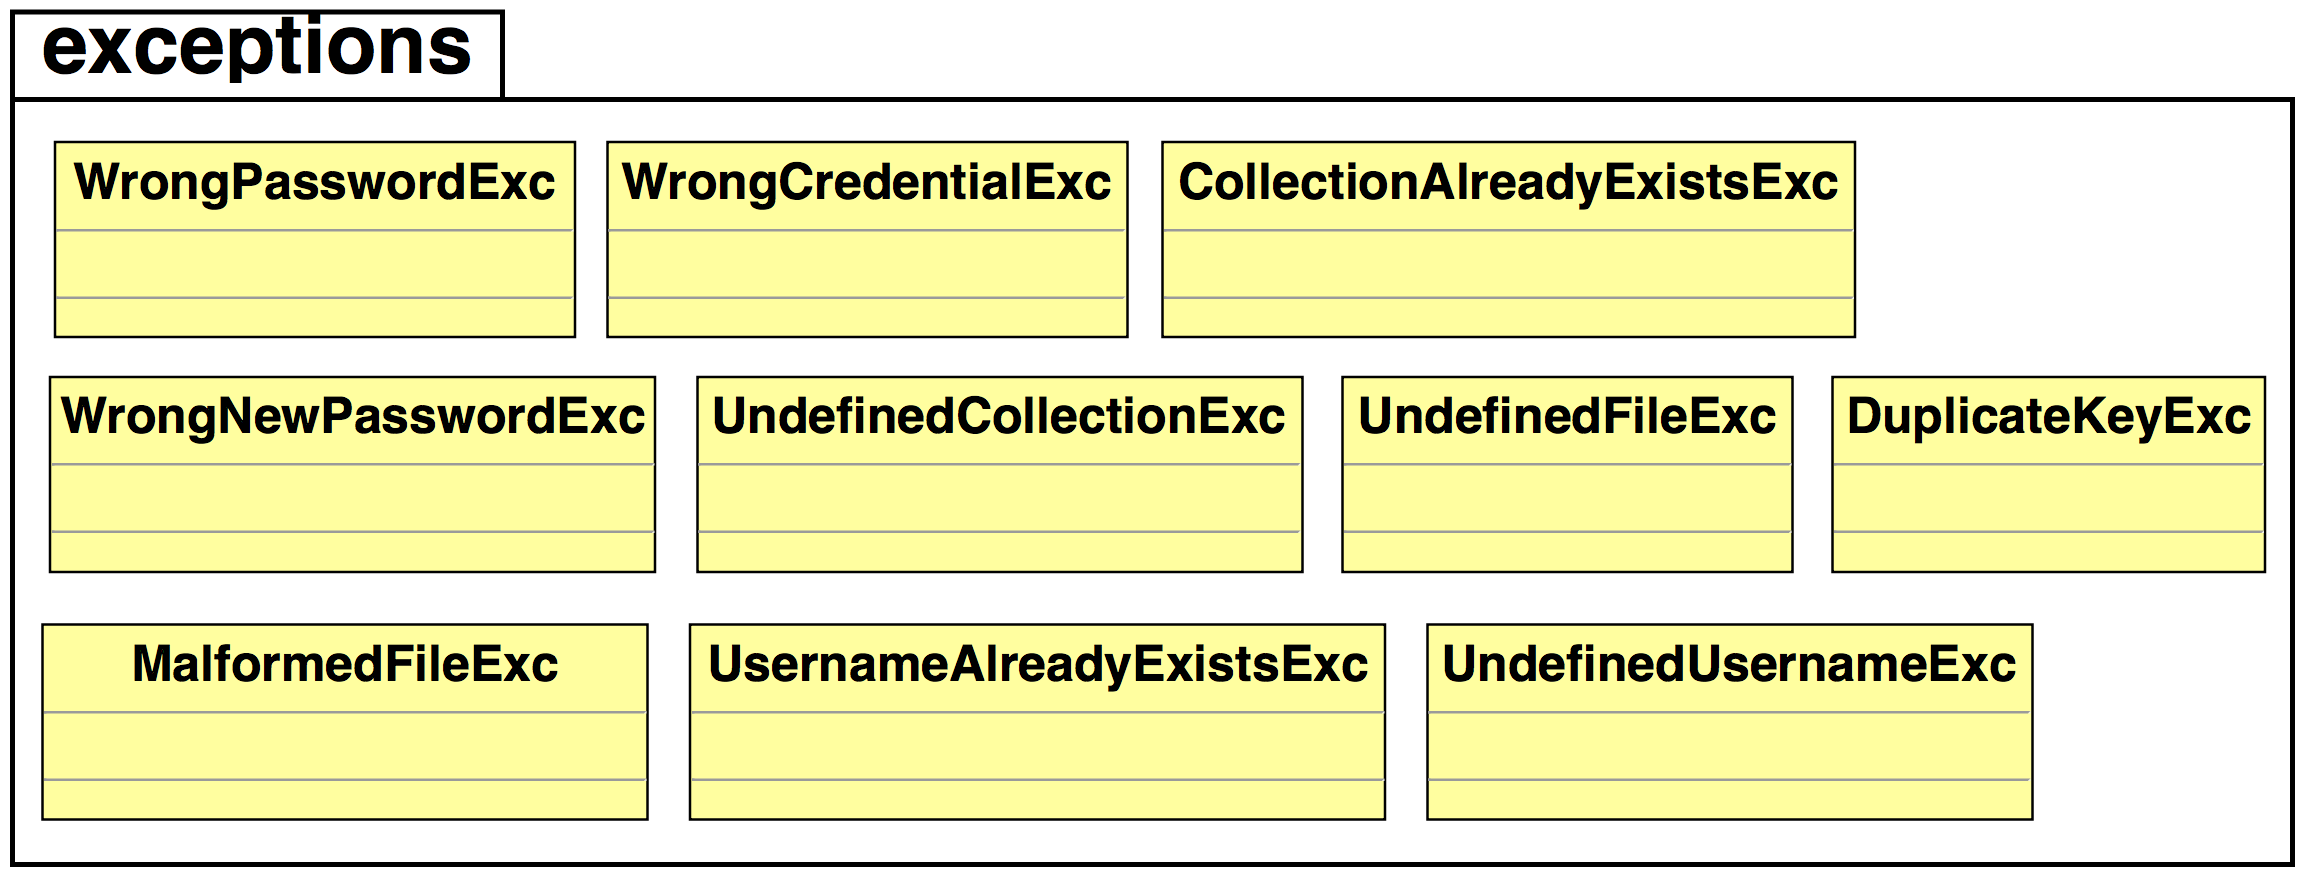
\includegraphics[width=0.7\textwidth,keepaspectratio]{RQ/Exceptions.png}
    \caption{Driver:Package exceptions}
  \end{center}
\end{figure}

\subsubsection{Descrizione}

\gloss{Package} che contiene le possibili eccezioni che si possono verificare nel \gloss{driver}

\subsubsection{Interazione con altre componenti}
\begin{itemize}
\item \hyperref[sec:actorbase::driver::client]{actorbase::driver::client};
\end{itemize}

\subsubsection{Classi}

\paragraph{actorbase::driver::exceptions::WrongCredentialExc}

\subparagraph{Descrizione}

Classe che rappresenta l'eccezione del tentativo di accesso con username o password sbagliati.

\subparagraph{Utilizzo}

Questa classe viene utilizzata dal \gloss{driver} per gestire errori nelle credenziali di accesso.


\paragraph{actorbase::driver::exceptions::WrongPasswordExc}

\subparagraph{Descrizione}

Classe che rappresenta l'eccezione dell'inserimento sbagliato della vecchia password.

\subparagraph{Utilizzo}

Questa classe viene utilizzata dal \gloss{driver} per gestire il caso in cui alla modifica della propria password, quando dovrei inserire la vecchia password questa non corrisponda.

\paragraph{actorbase::driver::exceptions::WrongNewPasswordExc}

\subparagraph{Descrizione}

Classe che rappresenta l'eccezione dell'inserimento sbagliato della nuova password.

\subparagraph{Utilizzo}

Questa classe viene utilizzata dal \gloss{driver} per gestire il caso in cui alla modifica della propria password, quando dovrei inserire la nuova password questa non soddisfi i requisiti richiesti.

\paragraph{actorbase::driver::exceptions::CollectionAlreadyExistsExc}

\subparagraph{Descrizione}

Classe che rappresenta l'eccezione del conflitto di nomi tra una collezione esistente e una nuova.

\subparagraph{Utilizzo}

Questa classe viene utilizzata dal \gloss{driver} per gestire il caso in cui alla creazione di una nuova collezione, il nome della nuova collezione corrisponda al nome di una collezione già esistente.

\paragraph{actorbase::driver::exceptions::UndefinedCollectionExc}

\subparagraph{Descrizione}

Classe che rappresenta l'eccezione di mancato inserimento del nome di una nuova collezione.

\subparagraph{Utilizzo}

Questa classe viene utilizzata dal \gloss{driver} per gestire il caso in cui alla creazione di una nuova collezione, venga omesso il nome di quest'ultima.

\paragraph{actorbase::driver::exceptions::UndefinedUsernameExc}

\subparagraph{Descrizione}

Classe che rappresenta l'eccezione di mancato inserimento dell'username utente.

\subparagraph{Utilizzo}

Questa classe viene utilizzata dal \gloss{driver} per gestire il caso in cui alla registrazione di un nuovo utente, venga omesso l'username.

\paragraph{actorbase::driver::exceptions::UsernameAlreadyExistsExc}

\subparagraph{Descrizione}

Classe che rappresenta l'eccezione del conflitto di username tra un utente già esistente e uno nuovo.

\subparagraph{Utilizzo}

Questa classe viene utilizzata dal \gloss{driver} per gestire il caso in cui alla registrazione di un nuovo utente, l'username di quest'ultimo corrisponda all'username di un utente già esistente.

\paragraph{actorbase::driver::exceptions::DuplicateKeyExc}

\subparagraph{Descrizione}

Classe che rappresenta l'eccezione del conflitto tra una chiave già esistente e una nuova chiave.

\subparagraph{Utilizzo}

Questa classe viene utilizzata dal \gloss{driver} per gestire il caso in cui all'inserimento di una nuova chiave, questa corrisponda ad una chiave già esistente nella stessa collezione.

\paragraph{actorbase::driver::exceptions::UndefinedFileExc}

\subparagraph{Descrizione}

Classe che rappresenta l'eccezione di inserimento di un path sbagliato di un file o del mancato inserimento del path.

\subparagraph{Utilizzo}

Questa classe viene utilizzata dal \gloss{driver} per gestire il caso in cui all'inserimento di un nuovo item o di una serie di item da file, si sbagli il path del file o si ometta di inserirlo.

\paragraph{actorbase::driver::exceptions::MalformedFileExc}

\subparagraph{Descrizione}

Classe che rappresenta l'eccezione di inserimento di un path di un file non conforme.

\subparagraph{Utilizzo}

Questa classe viene utilizzata dal \gloss{driver} per gestire il caso in cui all'inserimento di un nuovo item o di una serie di item da file, si inserisca il path di un file in un formato sbagliato o il cui testo non rispetta le regole di formattazione.


%%%%%%%%%%%%%%%%%%%%%%%%%%%%%%%%%%%%%%%%%%%%%%%%%%%%%%%%%%%%%%%%%%%%
% CLI PARTE                              %
%%%%%%%%%%%%%%%%%%%%%%%%%%%%%%%%%%%%%%%%%%%%%%%%%%%%%%%%%%%%%%%%%%%%

\subsection{actorbase::cli}
\label{sec:actorbase::cli}

\begin{figure}[H]
  \begin{center}
    \includegraphics[width=1.0\textwidth,keepaspectratio]{RP/CLI.png}
    \caption{CLI, architettura MVC variante push model}
  \end{center}
\end{figure}

\subsubsection{Descrizione}
\gloss{Package} per la parte di \gloss{client} rappresentata dalla \gloss{cli}.
Questa componente viene rappresentata usando il \gloss{design pattern}
\gloss{MVC} in versione \gloss{push model}.

\subsubsection{Interazioni con altre componenti}
\begin{itemize}
\item \hyperref[sec:actorbase::driver]{actorbase::driver}.
\end{itemize}

\subsubsection{Package contenuti}
\begin{itemize}
\item \hyperref[sec:actorbase::cli::views]{actorbase::cli::views};
\item \hyperref[sec:actorbase::cli::controllers]{actorbase::cli::controllers};
\item \hyperref[sec:actorbase::cli::models]{actorbase::cli::models}.
\end{itemize}

\subsection{actorbase::cli::views}
\label{sec:actorbase::cli::views}

\begin{figure}[H]
  \begin{center}
    \includegraphics[width=1.0\textwidth,keepaspectratio]{RP/CLI-view.png}
    \caption{CLI, views package, interazioni con Controllers e Models}
  \end{center}
\end{figure}

\subsubsection{Descrizione}

\gloss{Package} per la parte \gloss{view} della \gloss{cli}. Questa componente
gestisce l'output e offre l'interfaccia tramite cui l'utente può inserire i
comandi.

\subsubsection{Interfacce}

\paragraph{actorbase::cli::views::PromptProvider}
\label{sec:actorbase::cli::views::PromptProvider}

\subparagraph{Descrizione}
Interfaccia per la creazione del \gloss{prompt} dei comandi.

\subparagraph{Utilizzo}
Offre un'interfaccia per la creazione di un \gloss{prompt} generico.

\subparagraph{Realizzata da}
\begin{itemize}
\item actorbase::cli::views::ActorbasePrompt
\end{itemize}

\subparagraph{Metodi}
\begin{tabular}{| l | l | l | l |}
  \hline
  Nome & Accesso & Tipo di ritorno & Descrizione\\
  \hline
  getPrompt & public & String & Ritorna la stringa che rappresenta il \gloss{prompt}.\\
  \hline
\end{tabular}

\paragraph{actorbase::cli::views::Observer}
\label{sec:actorbase::cli::views::Observer}

\subparagraph{Descrizione}
Interfaccia per l'implementazione del \gloss{design pattern} \gloss{Observer}
che permette di aggiornare la \gloss{view} ad ogni risposta della componente
\gloss{driver}.

\subparagraph{Utilizzo}
Offre un'interfaccia per permettere di aggiornare la \gloss{view} ad ogni
risposta ricevuta dal \gloss{driver}.

\subparagraph{Realizzata da}
\begin{itemize}
\item actorbase::cli::views::ResultViewer
\end{itemize}

\subparagraph{Metodi}
\begin{tabular}{| l | l | l | l |}
  \hline
  Nome & Accesso & Tipo di ritorno & Descrizione\\
  \hline
  update & public & Unit & Aggiorna lo stato dell'observer\\
  \hline
\end{tabular}

\subparagraph{Parametri}
\begin{center}
  \textbf{update}
\end{center}
\begin{tabular}{| p{3cm} | p{3.5cm} | p{8.5cm} |}
  \hline
  Nome & Tipo & Descrizione\\
  \hline
  o & \hyperref[actorbase::cli::models::Observable]{Observable} & Rappresenta l'oggetto osservato\\
  \hline
\end{tabular}

\subsubsection{Classi}

\paragraph{actorbase::cli::views::CommandLoop}
\label{sec:actorbase::cli::views::CommandLoop}

\subparagraph{Descrizione}
Questa classe verrà utilizzata per leggere i comandi inseriti dall'utente.

\subparagraph{Utilizzo}
Viene utilizzata per la lettura dei comandi inseriti dall'utente.

\subparagraph{Attributi}
\begin{tabular}{| p{2.5cm} | p{1.5cm} | p{2cm} | p{2.5cm} | p{8.5cm} |}
  \hline
  Nome & Accesso & Mutabilità & Tipo & Descrizione\\
  \hline
  loop & private & immutabile & Boolean & Rappresenta la condizione do/while\\
  \hline
  commandInvoker & private & immutabile & CommandInvoker & Rappresenta il riferimento al model\\
  \hline
  view & private & immutabile & ResultViewer & Rappresenta il riferimento alla view\\
  \hline
  grammarParser & private & immutabile & GrammarParser & Rappresenta il riferimento al controller\\
  \hline
  reader & private & immutabile & ConsoleReader & Rappresenta il reader per console appplication \\
  \hline
  history & private & immutabile & FileHistory & Rappresenta il file contenente la storia dei comandi\\
  \hline
  prompt & private & immutabile & ActorbasePrompt & Rappresenta il prompt di Actorbase\\
  \hline
  banner & private & immutabile & ActorbaseBanner & Rappresenta il banner di Actorbase\\
  \hline
  completers & private & mutabile & List di String & Lista di stringhe che serve per suggerire i completamenti\\
  \hline
  out & private & immutabile & PrintWriter & Oggetto di tipo PrintWriter\\
  \hline
\end{tabular}

\paragraph{actorbase::cli::views::ActorbaseBanner}
\label{sec:actorbase::cli::views::ActorbaseBanner}

\subparagraph{Descrizione}

Classe per la creazione del \gloss{banner} da mostrare all'avvio della
\gloss{CLI}.

\subparagraph{Utilizzo}

Viene utilizzata per la creazione di un \gloss{banner} di presentazione
all'avvio della \gloss{CLI}.

\subparagraph{Metodi}

\begin{tabular}{| l | l | l | l |}
  \hline
  Nome & Accesso & Tipo di ritorno & Descrizione\\
  \hline
  getBanner & public & String & Crea il banner e lo ritorna come stringa\\
  \hline
\end{tabular}

\paragraph{actorbase::cli::views::ActorbasePrompt}
\label{sec:actorbase::cli::views::ActorbasePrompt}

\subparagraph{Descrizione}

Classe che implementa l'interfaccia \hyperref[sec:actorbase::cli::views::PromptProvider]{actorbase::cli::views::PromptProvider} per
la creazione di un \gloss{prompt} dei comandi.

\subparagraph{Utilizzo}

Viene utilizzata per la creazione di un \gloss{prompt} per l'inserimento dei
comandi e la visualizzazione delle informazioni relative alla connessione
effettuata.

\subparagraph{Classi ereditate}

\begin{itemize}
\item \hyperref[sec:actorbase::cli::views::PromptProvider]{actorbase::cli::views::PromptProvider}.
\end{itemize}

\subparagraph{Metodi}

\begin{tabular}{| l | l | l | l |}
  \hline
  Nome & Accesso & Tipo di ritorno & Descrizione\\
  \hline
  getPrompt & public & String & Ritorna la stringa che rappresenta il \gloss{prompt} di actorbase\\
  \hline
\end{tabular}

\subparagraph{Attributi}

\begin{tabular}{| p{2.5cm} | p{1.5cm} | p{2cm} | p{2.5cm} | p{8.5cm} |}
  \hline
  Nome & Accesso & Mutabilità & Tipo & Descrizione\\
  \hline
  os & private & immutabile & String & Oggetto che rappresenta il nome del sistema\\
  \hline
\end{tabular}

\paragraph{actorbase::cli::views::ResultViewer}
\label{sec:actorbase::cli::views::ResultViewer}

\subparagraph{Descrizione}

Classe per la gestione e la formattazione in output dei risultati ottenuti
dall'esecuzione del comando ricevuto in input tramite il \gloss{design
  pattern} \gloss{Observer}.

\subparagraph{Utilizzo}

Viene utilizzata per la gestione e la formattazione in output dei risultati
ottenuti dal server mediante l'inserimento dei comandi tramite il
\gloss{design pattern} \gloss{Observer}.

\subparagraph{Classi ereditate}

\begin{itemize}
\item \hyperref[sec:actorbase::cli::views::Observer]{actorbase::cli::views::Observer}.
\end{itemize}

\subparagraph{Metodi}
\begin{tabular}{| l | l | l | l |}
  \hline
  Nome & Accesso & Tipo di ritorno & Descrizione\\
  \hline
  update & public & Unit & Aggiorna lo stato della \gloss{view}\\
  \hline
\end{tabular}

\subparagraph{Parametri}

\begin{center}
  \textbf{update}
\end{center}
\begin{tabular}{| p{3cm} | p{3.5cm} | p{8.5cm} |}
  \hline
  Nome & Tipo & Descrizione\\
  \hline
  o & \hyperref[actorbase::cli::models::Observable]{Observable} & Rappresenta l'oggetto osservato\\
  \hline
\end{tabular}

\subsection{actorbase::cli::controllers}
\label{sec:actorbase::cli::controllers}

% TODO QUA MANCA L'IMMAGINE

\subsubsection{Descrizione}

\gloss{Package} per la parte \gloss{controller} della \gloss{cli}. Questa
componente si occupa di passare il comando ricevuto dalla \gloss{view} al
\gloss{model}.

\subsubsection{Classi}

\paragraph{actorbase::cli::controllers::GrammarParser}
\label{sec:actorbase::cli::controllers::GrammarParser}

\subparagraph{Descrizione}

Classe che si occupa di effettuare il \gloss{parsing} del comando ricevuto
dalla componente \gloss{view} e di chiamare la componente \gloss{model} con i
parametri opportuni.

\subparagraph{Utilizzo}

Viene utilizzata per effettuare il \gloss{parsing} del comando ricevuto da
\hyperref[sec:actorbase::cli::views::CommandLoop]{actorbase::cli::views::CommandLoop} e, in seguito, chiamare
\hyperref[sec:actorbase::cli::models::CommandInvoker]{actorbase::cli::models::CommandInvoker} con i parametri corretti per
l'esecuzione del comando.

\subparagraph{Metodi}

\begin{tabular}{| p{5.5cm} | p{1.5cm} | p{2cm} | p{7.5cm} |}
  \hline
  Nome & Accesso & Tipo di ritorno & Descrizione\\
  \hline
  authManagementCommand & public & Parser di \hyperref[sec:actorbase::cli::models::Command]{Command} & Fa il parsing del comando di autenticazione e istanzia il \hyperref[sec:actorbase::cli::models::LoginCommand]{LoginCommand} o il \hyperref[sec:actorbase::cli::models::LogoutCommand]{LogoutCommand} dedicato a seconda del caso\\
  \hline
  changePasswordCommand & public & Parser di \hyperref[sec:actorbase::cli::models::Command]{Command} & Fa il parsing del comando di cambio password e istanzia il \hyperref[sec:actorbase::cli::models::ChangePasswordCommand]{ChangePasswordCommand}\\
  \hline
  helpCommand & public & Parser di \hyperref[sec:actorbase::cli::models::Command]{Command} & Fa il parsing del comando di aiuto e istanzia l'\hyperref[sec:actorbase::cli::models::HelpCommand]{HelpCommand}\\
  \hline
  collectionManagementCommand & public & Parser di \hyperref[sec:actorbase::cli::models::Command]{Command} & Fa il parsing del comando di gestione delle collezioni e istanzia il \hyperref[sec:actorbase::cli::models::CreateCollectionCommand]{CreateCollectionCommand}, il \hyperref[sec:actorbase::cli::models::RemoveCollectionCommand]{RemoveCollectionCommand}, il \hyperref[sec:actorbase::cli::models::ListCollectionsCommand]{ListCollectionsCommand} o il \hyperref[sec:actorbase::cli::models::RenameCollectionCommand]{RenameCollectionCommand} a seconda del caso\\
  \hline
  addContributorCommand & public & Parser di \hyperref[sec:actorbase::cli::models::Command]{Command} & Fa il parsing del comando di aggiunta collaboratore e istanzia l'\hyperref[sec:actorbase::cli::models::AddContributorCommand]{AddContributorCommand}\\
  \hline
  removeContributorCommand & public & Parser di \hyperref[sec:actorbase::cli::models::Command]{Command} &
                                                                                                          Fa il parsing del comando di rimozione collaboratore e istanzia il \hyperref[sec:actorbase::cli::models::RemoveContributorCommand]{RemoveContributorCommand}\\
  \hline
  importExportCommand & public & Parser di \hyperref[sec:actorbase::cli::models::Command]{Command} & Fa il parsing del comando di import/export e istanzia l'\hyperref[sec:actorbase::cli::models::ImportCommand]{ImportCommand} o l'\hyperref[sec:actorbase::cli::models::ExportCommand]{ExportCommand} a seconda del caso\\
  \hline
  insertItemCommand & public & Parser di \hyperref[sec:actorbase::cli::models::Command]{Command} & Fa il parsing del comando di inserimento item e istanzia l'\hyperref[sec:actorbase::cli::models::InsertItemCommand]{InsertItemCommand}\\
  \hline
  removeItemCommand & public & Parser di \hyperref[sec:actorbase::cli::models::Command]{Command} &
                                                                                                   Fa il parsing del comando di rimozione item e istanzia il \hyperref[sec:actorbase::cli::models::RemoveItemCommand]{RemoveItemCommand}\\
  \hline
  findCommand & public & Parser di \hyperref[sec:actorbase::cli::models::Command]{Command} & Fa il parsing del comando di ricerca e istanzia il \hyperref[sec:actorbase::cli::models::FindCommand]{FindCommand}\\
  \hline
  userManagementCommand & public & Parser di \hyperref[sec:actorbase::cli::models::Command]{Command} & Fa il parsing del comando di gestione utente e istanzia l'\hyperref[sec:actorbase::cli::models::AddUserCommand]{AddUserCommand}, il \hyperref[sec:actorbase::cli::models::RemoveUserCommand]{RemoveUserCommand} o il \hyperref[sec:actorbase::cli::models::ResetPasswordCommand]{ResetPasswordCommand} a seconda del caso\\
  \hline
  commandList & public & Parser di \hyperref[sec:actorbase::cli::models::Command]{Command} & Racchiude tutti i possibili metodi di parsing\\
  \hline
  parseInput & public & Boolean & Metodo dedicato alla cattura dell'input a cui fare il parsing\\
  \hline
\end{tabular}

\subparagraph{Parametri}

\begin{center}
  \textbf{parserInput}
\end{center}
\begin{tabular}{| p{3cm} | p{3.5cm} | p{8.5cm} |}
  \hline
  Nome & Tipo & Descrizione\\
  \hline
  input & String & Stringa immessa dall'utente\\
  \hline
\end{tabular}

\subparagraph{Attributi}

\begin{tabular}{| p{2.5cm} | p{1.5cm} | p{2cm} | p{2.5cm} | p{8.5cm} |}
  \hline
  Nome & Accesso & Mutabilità & Tipo & Descrizione\\
  \hline
  types & private & immutabile & Parser[String] & Rappresenta i tipi accettati dalla shell\\
  \hline
  permissions & private & immutabile & Parser[String] & Rappresenta i permessi accettati dalla shell\\
  \hline
  quotedString & private & immutabile & Parser[String] & Rappresenta le Quoted String accettate dalla shell\\
  \hline
  literalString & private & immutabile & Parser[String] & Rappresenta le Stringhe letterali accettate dalla shell\\
  \hline
  listString & private & immutabile & Parser[String] & Rappresenta le ListString accettate dalla shell\\
  \hline
  keyString & private & immutabile & Parser[String] & Rappresenta le keyString accettate dalla shell\\
  \hline
\end{tabular}

\subsection{actorbase::cli::models}
\label{sec:actorbase::cli::models}

\subsubsection{Descrizione}

\gloss{Package} per la parte \gloss{model} della \gloss{cli}. Questa
componente si occupa della comunicazione con la componente \gloss{driver} e
con la componente \gloss{view} tramite il \gloss{push model} del \gloss{design
  pattern} \gloss{observer}. Per la gestione dei comandi si è scelto di
utilizzare il \gloss{command pattern}.

\subsubsection{Interfacce}

\paragraph{actorbase::cli::models::Command}
\label{sec:actorbase::cli::models::Command}

\subparagraph{Descrizione}

Interfaccia generica che rappresenta un comando.

\subparagraph{Utilizzo}

Viene utilizzata per offrire un'interfaccia comune a tutti i comandi.\\Ha un
riferimento a \hyperref[sec:actorbase::cli::models::CommandReceiver]{actorbase::cli::models::CommandReceiver} per l'esecuzione del
comando.

\subparagraph{Realizzata da}

\begin{itemize}
\item \hyperref[sec:actorbase::cli::models::AddContributorCommand]{actorbase::cli::models::AddContributorCommand};
\item \hyperref[sec:actorbase::cli::models::AddUserCommand]{actorbase::cli::models::AddUserCommand};
\item  \hyperref[sec:actorbase::cli::models::ChangePasswordCommand]{actorbase::cli::models::ChangePasswordCommand};
\item  \hyperref[sec:actorbase::cli::models::CreateCollectionCommand]{actorbase::cli::models::CreateCollectionCommand};
\item  \hyperref[sec:actorbase::cli::models::RemoveCollectionCommand]{actorbase::cli::models::RemoveCollectionCommand};
\item  \hyperref[sec:actorbase::cli::models::ExportCommand]{actorbase::cli::models::ExportCommand};
\item  \hyperref[sec:actorbase::cli::models::FindCommand]{actorbase::cli::models::FindCommand};
\item  \hyperref[sec:actorbase::cli::models::HelpCommand]{actorbase::cli::models::HelpCommand};
\item  \hyperref[sec:actorbase::cli::models::InsertItemCommand]{actorbase::cli::models::InsertItemCommand};
\item  \hyperref[sec:actorbase::cli::models::ListCollectionsCommand]{actorbase::cli::models::ListCollectionsCommand};
\item  \hyperref[sec:actorbase::cli::models::LoginCommand]{actorbase::cli::models::LoginCommand};
\item  \hyperref[sec:actorbase::cli::models::LogoutCommand]{actorbase::cli::models::LogoutCommand};
\item  \hyperref[sec:actorbase::cli::models::RemoveContributorCommand]{actorbase::cli::models::RemoveContributorCommand};
\item  \hyperref[sec:actorbase::cli::models::RemoveItemCommand]{actorbase::cli::models::RemoveItemCommand};
\item  \hyperref[sec:actorbase::cli::models::RemoveUserCommand]{actorbase::cli::models::RemoveUserCommand};
\item  \hyperref[sec:actorbase::cli::models::RenameCollectionCommand]{actorbase::cli::models::RenameCollectionCommand};
\item  \hyperref[sec:actorbase::cli::models::RemoveUserCommand]{actorbase::cli::models::RemoveUserCommand};
\item  \hyperref[sec:actorbase::cli::models::ResetPasswordCommand]{actorbase::cli::models::ResetPasswordCommand};
\end{itemize}

\subparagraph{Metodi}

\begin{tabular}{| l | l | l | l |}
  \hline
  Nome & Accesso & Tipo di ritorno & Descrizione\\
  \hline
  execute & public & String & Esegue il metodo\\
  \hline
\end{tabular}

\subsubsection{Classi}

\paragraph{actorbase::cli::models::Observable (abstract)}
\label{sec:actorbase::cli::models::Observable}

\subparagraph{Descrizione}

Classe astratta che rappresenta l'oggetto osservato nell'ambito del \gloss{design
  pattern} \gloss{observer}.

\subparagraph{Utilizzo}

Viene utilizzata per notificare la classe \hyperref[sec:actorbase::cli::views::Observer]{actorbase::cli::views::Observer}
quando avviene una modifica al proprio stato, ossia quando il \gloss{driver}
ha ritornato un risultato.

\subparagraph{Interazioni con altre classi}

\begin{itemize}
\item \hyperref[sec:actorbase::cli::views::Observer]{actorbase::cli::views::Observer}.
\end{itemize}

\subparagraph{Realizzata da}

\begin{itemize}
\item \hyperref[sec:actorbase::cli::models::CommandInvoker]{actorbase::cli::models::CommandInvoker}
\item \hyperref[sec:actorbase::cli::controllers::GrammarParser]{actorbase::cli::controllers::GrammarParser}
\end{itemize}

\subparagraph{Attributi}

\begin{tabular}{| p{1.5cm} | p{1.5cm} | p{2cm} | p{3.5cm} | p{8.5cm} |}
  \hline
  Nome & Accesso & Mutabilità & Tipo & Descrizione\\
  \hline
  observers & private & mutabile & ListBuffer[Observer] & Lista di oggetti che osservano questa classe\\
  \hline
  state & private & mutabile & String & Stato dell'oggetto\\
  \hline
\end{tabular}

\subparagraph{Metodi}

\begin{tabular}{| l | l | l | l |}
  \hline
  Nome & Accesso & Tipo di ritorno & Descrizione\\
  \hline
  setState & public & Unit & Cambia lo stato con quello in input\\
  \hline
  getState & public & String & Ritorna lo stato\\
  \hline
  attach & public & Unit & Aggiunge un observer\\
  \hline
  detach & public & Unit & Rimuove un observer\\
  \hline
  notifyAllObservers & public & Unit & Notifica tutti gli observers col proprio stato\\
  \hline
\end{tabular}

\subparagraph{Parametri}

\begin{center}
  \textbf{setState}
\end{center}
\begin{tabular}{| p{3cm} | p{3.5cm} | p{8.5cm} |}
  \hline
  Nome & Tipo & Descrizione\\
  \hline
  s & String & Stato da assegnare\\
  \hline
\end{tabular}

\begin{center}
  \textbf{attach}
\end{center}
\begin{tabular}{| p{3cm} | p{3.5cm} | p{8.5cm} |}
  \hline
  Nome & Tipo & Descrizione\\
  \hline
  observer & Observer & Observer da aggiungere all'oggetto\\
  \hline
\end{tabular}

\begin{center}
  \textbf{detach}
\end{center}
\begin{tabular}{| p{3cm} | p{3.5cm} | p{8.5cm} |}
  \hline
  Nome & Tipo & Descrizione\\
  \hline
  observer & Observer & Observer da rimuovere dall'oggetto\\
  \hline
\end{tabular}

\paragraph{actorbase::cli::models::CommandInvoker}
\label{sec:actorbase::cli::models::CommandInvoker}

\subparagraph{Descrizione}

Questa classe rappresenta l'\gloss{Invoker} del \gloss{command pattern}. Essa
si occupa di eseguire il comando ricevuto dalla componente \gloss{controller}.

\subparagraph{Utilizzo}

Viene utilizzata per eseguire il comando ricevuto da
\hyperref[sec:actorbase::cli::controllers::GrammarParser]{actorbase::cli::controllers::GrammarParser} chiamando il metodo opportuno che
implementa l'interfaccia \hyperref[sec:actorbase::cli::models::Command]{actorbase::cli::models::Command}.

\subparagraph{Classi ereditate}

\begin{itemize}
\item \hyperref[sec:actorbase::cli::models::Observable]{actorbase::cli::models::Observable}.
\end{itemize}

\subparagraph{Attributi}

\begin{tabular}{| p{2.5cm} | p{1.5cm} | p{2cm} | p{2.5cm} | p{8.5cm} |}
  \hline
  Nome & Accesso & Mutabilità & Tipo & Descrizione\\
  \hline
  history & private & mutabile & List[Command] & Una lista contenente la history dei comandi inseriti\\
  \hline
\end{tabular}

\subparagraph{Metodi}

\begin{tabular}{| l | l | l | l |}
  \hline
  Nome & Accesso & Tipo di ritorno & Descrizione\\
  \hline
  storeAndExecute & public & String & Immagazzina il comando nella history e provvede alla sua esecuzione\\
  \hline
\end{tabular}

\subparagraph{Parametri}

\begin{center}
  \textbf{setState}
\end{center}
\begin{tabular}{| p{3cm} | p{3.5cm} | p{8.5cm} |}
  \hline
  Nome & Tipo & Descrizione\\
  \hline
  cmd & Command & Comando da eseguire\\
  \hline
\end{tabular}

\paragraph{actorbase::cli::models::ChangePasswordCommand}
\label{sec:actorbase::cli::models::ChangePasswordCommand}

\subparagraph{Descrizione}

Classe per il comando di cambiamento password.

\subparagraph{Utilizzo}

Viene utilizzata per chiamare il metodo di
\hyperref[sec:actorbase::cli::models::CommandReceiver]{actorbase::cli::models::CommandReceiver} per il cambiamento della password.

\subparagraph{Classi ereditate}

\begin{itemize}
\item \hyperref[sec:actorbase::cli::models::Command]{actorbase::cli::models::Command}.
\end{itemize}

\subparagraph{Attributi}

\begin{tabular}{| p{1cm} | p{1.5cm} | p{2cm} | p{4cm} | p{8.5cm} |}
  \hline
  Nome & Accesso & Mutabilità & Tipo & Descrizione\\
  \hline
  cr & public & immutabile & CommandReceiver & Oggetto per l'esecuzione del comando\\
  \hline
\end{tabular}

\subparagraph{Metodi}

\begin{tabular}{| l | l | l | l |}
  \hline
  Nome & Accesso & Tipo di ritorno & Descrizione\\
  \hline
  execute & public & String & Provvede all'esecuzione del comando\\
  \hline
\end{tabular}


\paragraph{actorbase::cli::models::FindCommand}
\label{sec:actorbase::cli::models::FindCommand}

\subparagraph{Descrizione}

Classe per il comando di ricerca.

\subparagraph{Utilizzo}

Viene utilizzata per chiamare il metodo di
\hyperref[sec:actorbase::cli::models::CommandReceiver]{actorbase::cli::models::CommandReceiver} per la ricerca con i parametri immessi
dall'utente.

\subparagraph{Classi ereditate}

\begin{itemize}
\item \hyperref[sec:actorbase::cli::models::Command]{actorbase::cli::models::Command}.
\end{itemize}

\subparagraph{Attributi}

\begin{tabular}{| p{1cm} | p{1.5cm} | p{2cm} | p{4cm} | p{8.5cm} |}
  \hline
  Nome & Accesso & Mutabilità & Tipo & Descrizione\\
  \hline
  cr & public & immutabile & CommandReceiver & Oggetto per l'esecuzione del comando \\
  \hline
\end{tabular}

\subparagraph{Metodi}

\begin{tabular}{| l | l | l | l |}
  \hline
  Nome & Accesso & Tipo di ritorno & Descrizione\\
  \hline
  execute & public & String & Provvede all'esecuzione del comando\\
  \hline
\end{tabular}


\paragraph{actorbase::cli::models::HelpCommand}
\label{sec:actorbase::cli::models::HelpCommand}

\subparagraph{Descrizione}

Classe per il comando di aiunto.

\subparagraph{Utilizzo}
Viene utilizzata per chiamare il metodo di
\hyperref[sec:actorbase::cli::models::CommandReceiver]{actorbase::cli::models::CommandReceiver} per richiedere aiuto sulle possibili operazioni da fare.

\subparagraph{Classi ereditate}
\begin{itemize}
\item \hyperref[sec:actorbase::cli::models::Command]{actorbase::cli::models::Command}.
\end{itemize}

\subparagraph{Attributi}

\begin{tabular}{| p{1cm} | p{1.5cm} | p{2cm} | p{4cm} | p{8.5cm} |}
  \hline
  Nome & Accesso & Mutabilità & Tipo & Descrizione\\
  \hline
  cr & public & immutabile & CommandReceiver & Oggetto per l'esecuzione del comando \\
  \hline
\end{tabular}

\subparagraph{Metodi}

\begin{tabular}{| l | l | l | l |}
  \hline
  Nome & Accesso & Tipo di ritorno & Descrizione\\
  \hline
  execute & public & String & Provvede all'esecuzione del comando\\
  \hline
\end{tabular}

\paragraph{actorbase::cli::models::LogoutCommand}
\label{sec:actorbase::cli::models::LogoutCommand}

\subparagraph{Descrizione}

Classe per il comando di logout.

\subparagraph{Utilizzo}

Viene utilizzata per chiamare il metodo di
\hyperref[sec:actorbase::cli::models::CommandReceiver]{actorbase::cli::models::CommandReceiver} per il logout.

\subparagraph{Classi ereditate}

\begin{itemize}
\item \hyperref[sec:actorbase::cli::models::Command]{actorbase::cli::models::Command}.
\end{itemize}

\subparagraph{Attributi}

\begin{tabular}{| p{1cm} | p{1.5cm} | p{2cm} | p{4cm} | p{8.5cm} |}
  \hline
  Nome & Accesso & Mutabilità & Tipo & Descrizione\\
  \hline
  cr & public & immutabile & CommandReceiver & Oggetto per l'esecuzione del comando\\
  \hline
\end{tabular}

\subparagraph{Metodi}

\begin{tabular}{| l | l | l | l |}
  \hline
  Nome & Accesso & Tipo di ritorno & Descrizione\\
  \hline
  execute & public & String & Provvede all'esecuzione del comando\\
  \hline
\end{tabular}

\paragraph{actorbase::cli::models::ResetPasswordCommand}
\label{sec:actorbase::cli::models::ResetPasswordCommand}

\subparagraph{Descrizione}

Classe per il comando di reset della password.

\subparagraph{Utilizzo}

Viene utilizzata per chiamare il metodo di
\hyperref[sec:actorbase::cli::models::CommandReceiver]{actorbase::cli::models::CommandReceiver} per il reset della password
dell'utente specificato in input.

\subparagraph{Classi ereditate}

\begin{itemize}
\item \hyperref[sec:actorbase::cli::models::Command]{actorbase::cli::models::Command}.
\end{itemize}

\subparagraph{Attributi}

\begin{tabular}{| p{1cm} | p{1.5cm} | p{2cm} | p{4cm} | p{8.5cm} |}
  \hline
  Nome & Accesso & Mutabilità & Tipo & Descrizione\\
  \hline
  cr & public & immutabile & CommandReceiver & Oggetto per l'esecuzione del comando\\
  \hline
\end{tabular}

\subparagraph{Metodi}

\begin{tabular}{| l | l | l | l |}
  \hline
  Nome & Accesso & Tipo di ritorno & Descrizione\\
  \hline
  execute & public & String & Provvede all'esecuzione del comando\\
  \hline
\end{tabular}

\paragraph{actorbase::cli::models::ListCollectionsCommand}
\label{sec:actorbase::cli::models::ListCollectionsCommand}

\subparagraph{Descrizione}

Classe per il comando di visualizzazione dell'elenco dei nomi di tutte le
collezioni presenti nel \gloss{database}.

\subparagraph{Utilizzo}

Viene utilizzata per chiamare il metodo di
\hyperref[sec:actorbase::cli::models::CommandReceiver]{actorbase::cli::models::CommandReceiver} per la visualizzazione dell'elenco dei
nomi di tutte le collezioni presenti nel \gloss{database}.

\subparagraph{Classi ereditate}

\begin{itemize}
\item \hyperref[sec:actorbase::cli::models::Command]{actorbase::cli::models::Command}.
\end{itemize}

\subparagraph{Attributi}

\begin{tabular}{| p{1cm} | p{1.5cm} | p{2cm} | p{4cm} | p{8.5cm} |}
  \hline
  Nome & Accesso & Mutabilità & Tipo & Descrizione\\
  \hline
  cr & public & immutabile & CommandReceiver & Oggetto per l'esecuzione del comando\\
  \hline
\end{tabular}

\subparagraph{Metodi}

\begin{tabular}{| l | l | l | l |}
  \hline
  Nome & Accesso & Tipo di ritorno & Descrizione\\
  \hline
  execute & public & String & Provvede all'esecuzione del comando\\
  \hline
\end{tabular}

\paragraph{actorbase::cli::models::AddContributorCommand}
\label{sec:actorbase::cli::models::AddContributorCommand}

\subparagraph{Descrizione}

Classe per il comando di aggiunta collaboratore a una collezione.

\subparagraph{Utilizzo}

Viene utilizzata per chiamare il metodo di
\hyperref[sec:actorbase::cli::models::CommandReceiver]{actorbase::cli::models::CommandReceiver} per l'aggiunta di un collaboratore a
una collezione con il nome della \gloss{collezione} e lo username specificati
in input.

\subparagraph{Classi ereditate}

\begin{itemize}
\item \hyperref[sec:actorbase::cli::models::Command]{actorbase::cli::models::Command}.
\end{itemize}

\subparagraph{Attributi}

\begin{tabular}{| p{1cm} | p{1.5cm} | p{2cm} | p{4cm} | p{8.5cm} |}
  \hline
  Nome & Accesso & Mutabilità & Tipo & Descrizione\\
  \hline
  cr & public & immutabile & CommandReceiver & Oggetto per l'esecuzione del comando\\
  \hline
\end{tabular}

\subparagraph{Metodi}

\begin{tabular}{| l | l | l | l |}
  \hline
  Nome & Accesso & Tipo di ritorno & Descrizione\\
  \hline
  execute & public & String & Provvede all'esecuzione del comando\\
  \hline
\end{tabular}

\paragraph{actorbase::cli::models::LoginCommand}
\label{sec:actorbase::cli::models::LoginCommand}

\subparagraph{Descrizione}

Classe per il comando di login.

\subparagraph{Utilizzo}

Viene utilizzata per chiamare il metodo di
\hyperref[sec:actorbase::cli::models::CommandReceiver]{actorbase::cli::models::CommandReceiver} per il login con le credenziali
immesse dall'utente.

\subparagraph{Classi ereditate}

\begin{itemize}
\item \hyperref[sec:actorbase::cli::models::Command]{actorbase::cli::models::Command}.
\end{itemize}

\subparagraph{Attributi}

\begin{tabular}{| p{1cm} | p{1.5cm} | p{2cm} | p{4cm} | p{8.5cm} |}
  \hline
  Nome & Accesso & Mutabilità & Tipo & Descrizione\\
  \hline
  cr & public & immutabile & CommandReceiver & Oggetto per l'esecuzione del comando\\
  \hline
\end{tabular}

\subparagraph{Metodi}

\begin{tabular}{| l | l | l | l |}
  \hline
  Nome & Accesso & Tipo di ritorno & Descrizione\\
  \hline
  execute & public & String & Provvede all'esecuzione del comando\\
  \hline
\end{tabular}

\paragraph{actorbase::cli::models::RemoveCollectionCommand}
\label{sec:actorbase::cli::models::RemoveCollectionCommand}

\subparagraph{Descrizione}

Classe per il comando di rimozione una \gloss{collezione}.

\subparagraph{Utilizzo}

Viene utilizzata per chiamare il metodo di
\hyperref[sec:actorbase::cli::models::CommandReceiver]{actorbase::cli::models::CommandReceiver} per la rimozione di una collezione con
i parametri specificati in input.

\subparagraph{Classi ereditate}

\begin{itemize}
\item \hyperref[sec:actorbase::cli::models::Command]{actorbase::cli::models::Command}.
\end{itemize}

\subparagraph{Attributi}

\begin{tabular}{| p{1cm} | p{1.5cm} | p{2cm} | p{4cm} | p{8.5cm} |}
  \hline
  Nome & Accesso & Mutabilità & Tipo & Descrizione\\
  \hline
  cr & public & immutabile & CommandReceiver & Oggetto per l'esecuzione del comando\\
  \hline
\end{tabular}

\subparagraph{Metodi}

\begin{tabular}{| l | l | l | l |}
  \hline
  Nome & Accesso & Tipo di ritorno & Descrizione\\
  \hline
  execute & public & String & Provvede all'esecuzione del comando\\
  \hline
\end{tabular}

\paragraph{actorbase::cli::models::RemoveContributorCommand}
\label{sec:actorbase::cli::models::RemoveContributorCommand}

\subparagraph{Descrizione}

Classe per il comando di rimozione di un collaboratore da una collezione.

\subparagraph{Utilizzo}

Viene utilizzata per chiamare il metodo di
\hyperref[sec:actorbase::cli::models::CommandReceiver]{actorbase::cli::models::CommandReceiver} per la rimozione di un collaboratore
da una collezione con con il nome della \gloss{collezione} e lo username
specificati in input.

\subparagraph{Classi ereditate}

\begin{itemize}
\item \hyperref[sec:actorbase::cli::models::Command]{actorbase::cli::models::Command}.
\end{itemize}

\subparagraph{Attributi}

\begin{tabular}{| p{1cm} | p{1.5cm} | p{2cm} | p{4cm} | p{8.5cm} |}
  \hline
  Nome & Accesso & Mutabilità & Tipo & Descrizione\\
  \hline
  cr & public & immutabile & CommandReceiver & Oggetto per l'esecuzione del comando\\
  \hline
\end{tabular}

\subparagraph{Metodi}

\begin{tabular}{| l | l | l | l |}
  \hline
  Nome & Accesso & Tipo di ritorno & Descrizione\\
  \hline
  execute & public & String & Provvede all'esecuzione del comando\\
  \hline
\end{tabular}

\paragraph{actorbase::cli::models::RenameCollectionCommand}
\label{sec:actorbase::cli::models::RenameCollectionCommand}

\subparagraph{Descrizione}

Classe per il comando rinominazione di una \gloss{collezione}.

\subparagraph{Utilizzo}

Viene utilizzata per chiamare il metodo di \hyperref[sec:actorbase::cli::models::CommandReceiver]{actorbase::cli::models::CommandReceiver} per la rinominazione di una \gloss{collezione} con i parametri specificati in input.

\subparagraph{Classi ereditate}

\begin{itemize}
\item \hyperref[sec:actorbase::cli::models::Command]{actorbase::cli::models::Command}.
\end{itemize}

\subparagraph{Attributi}

\begin{tabular}{| p{1cm} | p{1.5cm} | p{2cm} | p{4cm} | p{8.5cm} |}
  \hline
  Nome & Accesso & Mutabilità & Tipo & Descrizione\\
  \hline
  cr & public & immutabile & CommandReceiver & Oggetto per l'esecuzione del comando\\
  \hline
\end{tabular}

\subparagraph{Metodi}

\begin{tabular}{| l | l | l | l |}
  \hline
  Nome & Accesso & Tipo di ritorno & Descrizione\\
  \hline
  execute & public & String & Provvede all'esecuzione del comando\\
  \hline
\end{tabular}

\paragraph{actorbase::cli::models::AddUserCommand}
\label{sec:actorbase::cli::models::AddUserCommand}

\subparagraph{Descrizione}
Classe per il comando di aggiunta di un utente.

\subparagraph{Utilizzo}

Viene utilizzata per chiamare il metodo di
\hyperref[sec:actorbase::cli::models::CommandReceiver]{actorbase::cli::models::CommandReceiver} per l'aggiunta di un utente con i
parametri specificati in input.

\subparagraph{Classi ereditate}

\begin{itemize}
\item \hyperref[sec:actorbase::cli::models::Command]{actorbase::cli::models::Command}.
\end{itemize}

\subparagraph{Attributi}

\begin{tabular}{| p{1cm} | p{1.5cm} | p{2cm} | p{4cm} | p{8.5cm} |}
  \hline
  Nome & Accesso & Mutabilità & Tipo & Descrizione\\
  \hline
  cr & public & immutabile & CommandReceiver & Oggetto per l'esecuzione del comando\\
  \hline
\end{tabular}

\subparagraph{Metodi}

\begin{tabular}{| l | l | l | l |}
  \hline
  Nome & Accesso & Tipo di ritorno & Descrizione\\
  \hline
  execute & public & String & Provvede all'esecuzione del comando\\
  \hline
\end{tabular}

\paragraph{actorbase::cli::models::HelpCommand}
\label{sec:actorbase::cli::models::HelpCommand}

\subparagraph{Descrizione}
Classe per la richiesta di aiuto.

\subparagraph{Utilizzo}

Viene utilizzata per chiamare il metodo di
actorbase::cli::models::CommandReceiver per la richiesta di aiuto con i
parametri immessi dall'utente.

\subparagraph{Classi ereditate}

\begin{itemize}
\item \hyperref[sec:actorbase::cli::models::Command]{actorbase::cli::models::Command}.
\end{itemize}

\subparagraph{Attributi}

\begin{tabular}{| p{1cm} | p{1.5cm} | p{2cm} | p{4cm} | p{8.5cm} |}
  \hline
  Nome & Accesso & Mutabilità & Tipo & Descrizione\\
  \hline
  cr & public & immutabile & CommandReceiver & Oggetto per l'esecuzione del comando\\
  \hline
\end{tabular}

\subparagraph{Metodi}

\begin{tabular}{| l | l | l | l |}
  \hline
  Nome & Accesso & Tipo di ritorno & Descrizione\\
  \hline
  execute & public & String & Provvede all'esecuzione del comando\\
  \hline
\end{tabular}

\paragraph{actorbase::cli::models::RemoveItemCommand}
\label{sec:actorbase::cli::models::RemoveItemCommand}

\subparagraph{Descrizione}

Classe per il comando di rimozione di un \gloss{item}.

\subparagraph{Utilizzo}

Viene utilizzata per chiamare il metodo di
\hyperref[sec:actorbase::cli::models::CommandReceiver]{actorbase::cli::models::CommandReceiver} per la rimozione di un \gloss{item}
con i parametri immessi dall'utente.

\subparagraph{Classi ereditate}

\begin{itemize}
\item \hyperref[sec:actorbase::cli::models::Command]{actorbase::cli::models::Command}.
\end{itemize}

\subparagraph{Attributi}

\begin{tabular}{| p{1cm} | p{1.5cm} | p{2cm} | p{4cm} | p{8.5cm} |}
  \hline
  Nome & Accesso & Mutabilità & Tipo & Descrizione\\
  \hline
  cr & public & immutabile & CommandReceiver & Oggetto per l'esecuzione del comando\\
  \hline
\end{tabular}

\subparagraph{Metodi}

\begin{tabular}{| l | l | l | l |}
  \hline
  Nome & Accesso & Tipo di ritorno & Descrizione\\
  \hline
  execute & public & String & Provvede all'esecuzione del comando\\
  \hline
\end{tabular}

\paragraph{actorbase::cli::models::RemoveUserCommand}
\label{sec:actorbase::cli::models::RemoveUserCommand}

\subparagraph{Descrizione}

Classe per il comando di rimozione di un utente.

\subparagraph{Utilizzo}

Viene utilizzata per chiamare il metodo di
\hyperref[sec:actorbase::cli::models::CommandReceiver]{actorbase::cli::models::CommandReceiver} per la rimozione di un utente con i
parametri immessi dall'utente.

\subparagraph{Classi ereditate}

\begin{itemize}
\item \hyperref[sec:actorbase::cli::models::Command]{actorbase::cli::models::Command}.
\end{itemize}

\subparagraph{Attributi}

\begin{tabular}{| p{1cm} | p{1.5cm} | p{2cm} | p{4cm} | p{8.5cm} |}
  \hline
  Nome & Accesso & Mutabilità & Tipo & Descrizione\\
  \hline
  cr & public & immutabile & CommandReceiver & Oggetto per l'esecuzione del comando\\
  \hline
\end{tabular}

\subparagraph{Metodi}

\begin{tabular}{| l | l | l | l |}
  \hline
  Nome & Accesso & Tipo di ritorno & Descrizione\\
  \hline
  execute & public & String & Provvede all'esecuzione del comando\\
  \hline
\end{tabular}

\paragraph{actorbase::cli::models::ImportCommand}
\label{sec:actorbase::cli::models::ImportCommand}

\subparagraph{Descrizione}

Classe per il comando di importazione da un file \gloss{JSON}.

\subparagraph{Utilizzo}

Viene utilizzata per chiamare il metodo di
\hyperref[sec:actorbase::cli::models::CommandReceiver]{actorbase::cli::models::CommandReceiver} per l'importazione da un file
\gloss{JSON} con i parametri immessi dall'utente.

\subparagraph{Classi ereditate}

\begin{itemize}
\item \hyperref[sec:actorbase::cli::models::Command]{actorbase::cli::models::Command}.
\end{itemize}

\subparagraph{Attributi}
\begin{tabular}{| p{1cm} | p{1.5cm} | p{2cm} | p{4cm} | p{8.5cm} |}
  \hline
  Nome & Accesso & Mutabilità & Tipo & Descrizione\\
  \hline
  cr & public & immutabile & CommandReceiver & Oggetto per l'esecuzione del comando\\
  \hline
\end{tabular}

\subparagraph{Metodi}

\begin{tabular}{| l | l | l | l |}
  \hline
  Nome & Accesso & Tipo di ritorno & Descrizione\\
  \hline
  execute & public & String & Provvede all'esecuzione del comando\\
  \hline
\end{tabular}

\paragraph{actorbase::cli::models::InsertItemCommand}
\label{sec:actorbase::cli::models::InsertItemCommand}

\subparagraph{Descrizione}

Classe per il comando di inserimento di un \gloss{item} in una
\gloss{collezione}.

\subparagraph{Utilizzo}

Viene utilizzata per chiamare il metodo di \hyperref[sec:actorbase::cli::models::CommandReceiver]{actorbase::cli::models::CommandReceiver} per l' inserimento di un \gloss{item} in una \gloss{collezione} con i parametri immessi dall'utente.

\subparagraph{Classi ereditate}

\begin{itemize}
\item \hyperref[sec:actorbase::cli::models::Command]{actorbase::cli::models::Command}.
\end{itemize}

\subparagraph{Attributi}

\begin{tabular}{| p{1cm} | p{1.5cm} | p{2cm} | p{4cm} | p{8.5cm} |}
  \hline
  Nome & Accesso & Mutabilità & Tipo & Descrizione\\
  \hline
  cr & public & immutabile & CommandReceiver & Oggetto per l'esecuzione del comando\\
  \hline
\end{tabular}

\subparagraph{Metodi}

\begin{tabular}{| l | l | l | l |}
  \hline
  Nome & Accesso & Tipo di ritorno & Descrizione\\
  \hline
  execute & public & String & Provvede all'esecuzione del comando\\
  \hline
\end{tabular}

\paragraph{actorbase::cli::models::CreateCollectionCommand}
\label{sec:actorbase::cli::models::CreateCollectionCommand}

\subparagraph{Descrizione}

Classe per il comando di creazione di una nuova \gloss{collezione}.

\subparagraph{Utilizzo}

Viene utilizzata per chiamare il metodo di
\hyperref[sec:actorbase::cli::models::CommandReceiver]{actorbase::cli::models::CommandReceiver} per la creazione di una nuova
\gloss{collezione} con i parametri immessi dall'utente.

\subparagraph{Classi ereditate}

\begin{itemize}
\item \hyperref[sec:actorbase::cli::models::Command]{actorbase::cli::models::Command}.
\end{itemize}

\subparagraph{Attributi}

\begin{tabular}{| p{1cm} | p{1.5cm} | p{2cm} | p{4cm} | p{8.5cm} |}
  \hline
  Nome & Accesso & Mutabilità & Tipo & Descrizione\\
  \hline
  cr & public & immutabile & CommandReceiver & Oggetto per l'esecuzione del comando\\
  \hline
\end{tabular}

\subparagraph{Metodi}

\begin{tabular}{| l | l | l | l |}
  \hline
  Nome & Accesso & Tipo di ritorno & Descrizione\\
  \hline
  execute & public & String & Provvede all'esecuzione del comando\\
  \hline
\end{tabular}

\paragraph{actorbase::cli::models::ExportCommand}
\label{sec:actorbase::cli::models::ExportCommand}

\subparagraph{Descrizione}

Classe per il comando di esportazione in file \gloss{JSON}.

\subparagraph{Utilizzo}

Viene utilizzata per chiamare il metodo di
\hyperref[sec:actorbase::cli::models::CommandReceiver]{actorbase::cli::models::CommandReceiver} per l'esportazione in file
\gloss{JSON} con i parametri immessi dall'utente.

\subparagraph{Classi ereditate}

\begin{itemize}
\item \hyperref[sec:actorbase::cli::models::Command]{actorbase::cli::models::Command}.
\end{itemize}

\subparagraph{Attributi}

\begin{tabular}{| p{1cm} | p{1.5cm} | p{2cm} | p{4cm} | p{8.5cm} |}
  \hline
  Nome & Accesso & Mutabilità & Tipo & Descrizione\\
  \hline
  cr & public & immutabile & CommandReceiver & Oggetto per l'esecuzione del comando\\
  \hline
\end{tabular}

\subparagraph{Metodi}

\begin{tabular}{| l | l | l | l |}
  \hline
  Nome & Accesso & Tipo di ritorno & Descrizione\\
  \hline
  execute & public & String & Provvede all'esecuzione del comando\\
  \hline
\end{tabular}

\paragraph{actorbase::cli::models::CommandReceiver}
\label{sec:actorbase::cli::models::CommandReceiver}

\subparagraph{Descrizione}

Classe contenente i metodi per richiamare la componente \gloss{driver} per
l'esecuzione dei comandi o per restituire l'aiuto se richiesto.

\subparagraph{Utilizzo}

Viene utilizzata da \hyperref[sec:actorbase::cli::models::Command]{actorbase::cli::models::Command} per chiamare
\hyperref[sec:actorbase::driver::client::ActorbaseClient]{actorbase::driver::client::ActorbaseClient} o per ricevere un aiuto da
visualizzare se richiesto dall'utente.

\subparagraph{Interazioni con altre classi}

\begin{itemize}
\item \hyperref[sec:actorbase::cli::models::Command]{actorbase::cli::models::Command};
\item \hyperref[sec:actorbase::driver::client::ActorbaseClient]{actorbase::driver::client::ActorbaseClient}.
\end{itemize}

\subparagraph{Attributi}

\begin{tabular}{| p{2.5cm} | p{1.5cm} | p{2cm} | p{2.5cm} | p{8.5cm} |}
  \hline
  Nome & Accesso & Mutabilità & Tipo & Descrizione\\
  \hline
  actorbaseDriver & public & mutabile & ActorbaseDriver & Istanza di \hyperref[sec:actorbase::driver::]{ActorbaseDriver} usata per l'esecuzione del comandi\\
  \hline
  params & public & immutabile & Map[Any,Any] & Parametri inseriti dall'utente per l'esecuzione dei comandi\\
  \hline
\end{tabular}

\subparagraph{Metodi}

\begin{tabular}{| l | l | l | l |}
  \hline
  Nome & Accesso & Ritorno & Descrizione\\
  \hline
  insert & public & String & Metodo per richiamare il comando di inserimento del driver\\
  \hline
  removeItem & public & String & Metodo per richiamare il comando di rimozione Item del driver\\
  \hline
  export & public & String & Metodo per richiamare il comando di esportazione su file del driver\\
  \hline
  login & public & String & Metodo per richiamare il comando di login del driver\\
  \hline
  logout & public & String & Metodo per richiamare il comando di logout del driver\\
  \hline
  find & public & String & Metodo per richiamare il comando di ricerca di items del driver\\
  \hline
  help & public & String & Metodo per il comando di aiuto\\
  \hline
  createCollection & public & String & Metodo per richiamare il comando di creazione collezione del driver\\
  \hline
  listCollections & public & String & Metodo per richiamare il metodo di lista collezioni del driver\\
  \hline
  renameCollection & public & String & Metodo per richiamare il metodo di rinomina collezione del driver\\
  \hline
  deleteCollection & public & String & Metodo per richiamare il metodo di rimozione collezione del driver\\
  \hline
  addContributor & public & String & Metodo per richiamare il metodo di aggiunta collaboratore del driver\\
  \hline
  removeContributor & public & String & Metodo per richiamare il metodo di rimozione collaboratore del driver\\
  \hline
  changePassword & public & String & Metodo per richiamare il metodo di cambio password del driver\\
  \hline
  addUser & public & String & Metodo per richiamare il metodo di aggiunta utente del driver\\
  \hline
  removeUser & public & String & Metodo per richiamare il metodo di rimozione utente del driver\\
  \hline
  resetPassword & public & String & Metodo per richiamare il metodo di reset password del driver\\
  \hline
\end{tabular}

\section{Diagrammi di Sequenza}

In questa sezione, vengono illustrati i diagrammi di sequenza che descrivono
le interazioni tra le varie componenti del sistema e in particolare lo scambio
di messaggi che avviene tra gli attori nella componente server di actorbase.\\
Sono stati creati dai \textit{Progettisti} diversi diagrammi con diversi livelli
di astrazione.\\
Per semplificare i diagrammi, evitare ripetitività e migliorare la leggibilità di
questi, nella maggior parte dei seguenti l'input sarà dato dalla componente \gloss{Driver}. In un utilizzo reale sarà un utente che utilizza il \gloss{Driver} o la
\gloss{CLI} che darà l'input iniziale.

\subsection{Interazioni generali tra componenti}
Questo diagramma rappresenta l'interazione generale tra le tre componenti che
compongono il sistema actorbase.\\
L'utente è connesso alla \gloss{CLI} e inserisce un comando. A questo punto la
componente \gloss{CLI} (se non è instanziato un \gloss{Driver} lo crea per poi
utilizzarlo) utilizza il \gloss{Driver} per richiamare il metodo relativo al
comando inserito dall'utente.\\Il \gloss{Driver} provvederà a tradurre il
comando coi relativi parametri immessi dall'utente in una stringa
\hyperref[sec:RESP]{RESP} e la invierà al server attraverso un \gloss{socket
  tcp}. Il server provvederà a fare le elaborazioni richieste attraverso l'uso
degli attori e quando queste saranno finite risponderà al \gloss{Driver}
mandando via \gloss{socket tcp} una stringa \hyperref[sec:RESP]{RESP} che a sua
volta provvederà a trasformarla in un
\hyperref[sec:driver::actorbasedata::actorbaseobject]{actorbase object} e lo
restituirà al suo utilizzatore.
\begin{figure}[H]
  \begin{center}
    \includegraphics[width=0.9\textwidth, keepaspectratio]{img/diagrammiSequenza/ScambioMessaggiGenerico.png}
    \caption{Diagramma di sequenza - Interazioni generali tra componenti}
  \end{center}
\end{figure}

\subsection{Inserimento di un Item}

Questo diagramma rappresenta l'interazione tra le componenti nel caso di una richiesta di inserimento di un \gloss{item}.\\
La componente \hyperref[sec:actorbase::driver::client::Connection]{actorbase::driver::client::Connection}
manda tramite \gloss{socket tcp} al \hyperref[sec:actorbase::actorsystem::clientactor::ClientActor]{actorbase::actorsystem::clientactor::ClientActor}
una stringa \hyperref[sec:RESP]{RESP} contenente il comando di inserimento \gloss{item} con
i parametri.\\
Da questo componente parte il messaggio di Insert(key, value) ad un \hyperref[sec:actorbase::actorsystem::clientactor::MainActor]{actorbase::actorsystem::clientactor::MainActor} scelto in base ad una
politica di \gloss{routing}. Il MainActor manderà un messaggio allo \hyperref[sec:actorbase::actorsystem::clientactor::StoreFinder]{actorbase::actorsystem::clientactor::StoreFinder} relativo il quale manderà un messaggio allo \hyperref[sec:actorbase::actorsystem::clientactor::StoreKeeper]{actorbase::actorsystem::clientactor::StoreKeeper} che dovrà salvarsi l'informazione
sulla propria mappa.\\
A questo punto lo Storekeeper manderà un messaggio al \gloss{ClientActor} con la risposta
(positiva o negativa che sia) il quale risponderà sempre tramite \gloss{socket tcp} al \gloss{Driver} con una stringa RESP.
\begin{figure}[H]
  \begin{center}
    \includegraphics[width=0.9\textwidth, keepaspectratio]{img/diagrammiSequenza/esempioInsert.png}
    \caption{Diagramma di sequenza - Inserimento di un item}
  \end{center}
\end{figure}

\subsection{Inserimento di un Item con Storekeeper pieno}

Questo diagramma rappresenta l'interazione tra le componenti nel caso di una richiesta di inserimento di un \gloss{item} in uno Storekeeper con una mappa piena.\\
La componente \hyperref[sec:actorbase::driver::client::Connection]{actorbase::driver::client::Connection}
manda tramite \gloss{socket tcp} al \hyperref[sec:actorbase::actorsystem::clientactor::ClientActor]{actorbase::actorsystem::clientactor::ClientActor}
una stringa \hyperref[sec:RESP]{RESP} contenente il comando di inserimento \gloss{item} con
i parametri.\\
Da questo componente parte il messaggio di Insert(key, value) ad un \hyperref[sec:actorbase::actorsystem::clientactor::MainActor]{actorbase::actorsystem::clientactor::MainActor} scelto in base ad una
politica di \gloss{routing}. Il MainActor manderà un messaggio allo \hyperref[sec:actorbase::actorsystem::clientactor::StoreFinder]{actorbase::actorsystem::clientactor::StoreFinder} relativo il quale manderà un messaggio allo \hyperref[sec:actorbase::actorsystem::clientactor::StoreKeeper]{actorbase::actorsystem::clientactor::StoreKeeper} che essendo pieno manda un
messaggio DuplicateRequestSK contenente metà della propria mappa e una ActorRef del proprio parent ad un \hyperref[sec:actorbase::actorsystem::clientactor::Manager]{actorbase::actorsystem::clientactor::Manager}. Il Manager inoltra il messaggio DuplicateRequestSK al parent dello Storekeeper precedentemente coinvolto. Questo Storefinder infine creerà un nuovo Storekeeper con il pezzo di mappa ricevuto. \\
A questo punto il nuovo Storekeeper manderà un messaggio al \gloss{ClientActor} con
la risposta (positiva o negativa che sia) il quale risponderà sempre tramite
\gloss{socket tcp} al \gloss{Driver} con una stringa RESP.
\begin{figure}[H]
  \begin{center}
    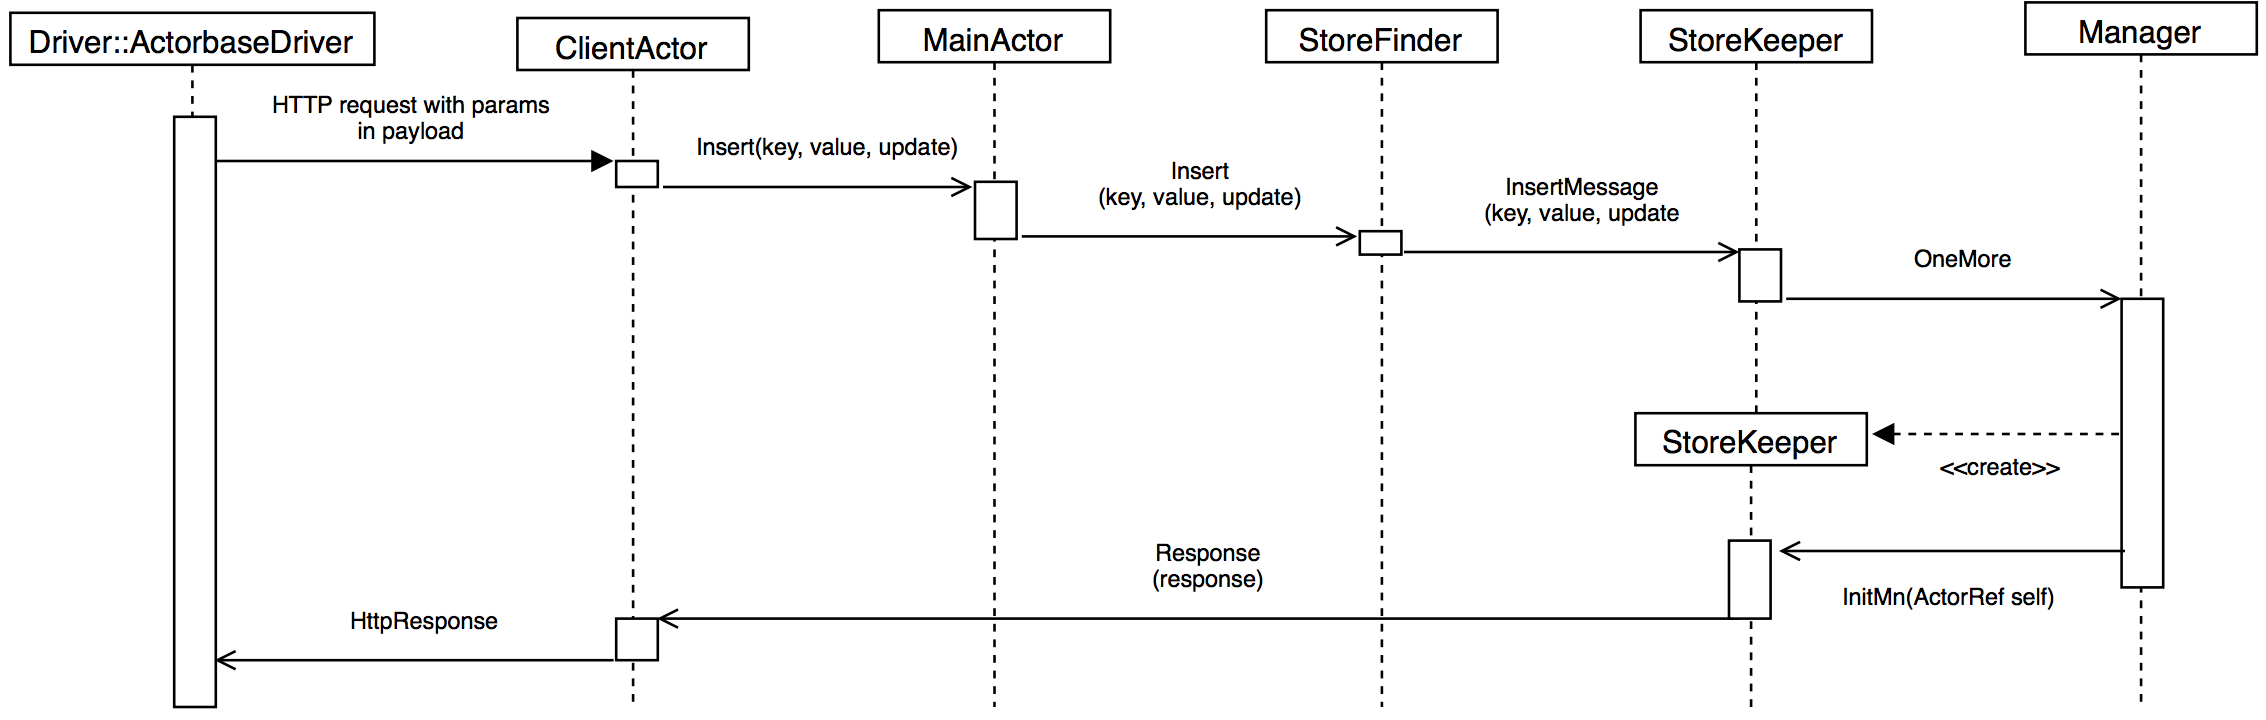
\includegraphics[width=0.9\textwidth, keepaspectratio]{img/diagrammiSequenza/esempioInsertFull.png}
    \caption{Diagramma di sequenza - Inserimento di un item}
  \end{center}
\end{figure}

\subsection{Autenticazione}

Questo diagramma rappresenta l'interazione tra le componenti nel caso di una richiesta di autenticazione di un utente.\\
La componente \hyperref[sec:actorbase::driver::client::Connection]{actorbase::driver::client::Connection}
manda tramite \gloss{socket tcp} al \hyperref[sec:actorbase::actorsystem::clientactor::ClientActor]{actorbase::actorsystem::clientactor::ClientActor}
una stringa \hyperref[sec:RESP]{RESP} contenente il comando di inserimento \gloss{item} con
i parametri.\\
Da questo componente parte il messaggio di GetItemFrom(UsersCollection, Username) ad un \hyperref[sec:actorbase::actorsystem::clientactor::MainActor]{actorbase::actorsystem::clientactor::MainActor} scelto in base ad una
politica di \gloss{routing}. Il MainActor manderà un messaggio allo \hyperref[sec:actorbase::actorsystem::clientactor::StoreFinder]{actorbase::actorsystem::clientactor::StoreFinder} relativo il quale manderà un messaggio getPassword(username) allo \hyperref[sec:actorbase::actorsystem::clientactor::UserKeeper]{actorbase::actorsystem::clientactor::UserKeeper}. Quest'ultimo risponderà al \gloss{ClientActor} con un messaggio loginResponse contenente la password relativa allo username richiesto.\\
Il \gloss{ClientActor} eseguirà un confronto tra la password immessa dall'utente e la password ritornata dallo Userkeeper. In caso positivo cambierà il proprio stato
e risponderà al \gloss{Driver} con un messaggio che indica un esito positivo. In caso negativo resterà nello stato attuale e manderà un messaggio al \gloss{Driver} che indica un esito negativo.
\begin{figure}[H]
  \begin{center}
    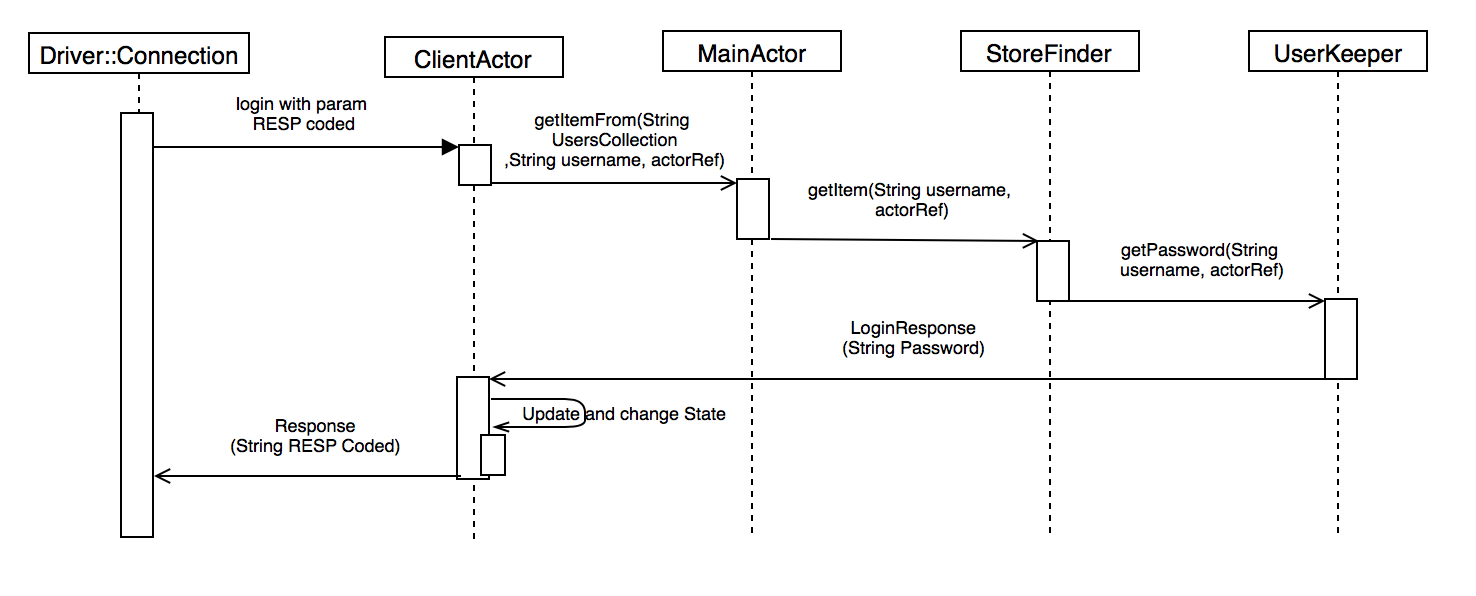
\includegraphics[width=0.9\textwidth, keepaspectratio]{img/diagrammiSequenza/esempioAuth.png}
    \caption{Diagramma di sequenza - Autenticazione}
  \end{center}
\end{figure}

\subsection{Salvataggio su filesystem}

Questo diagramma rappresenta l'interazione tra le componenti nel caso venga
effettuato un salvataggio dei dati su filesystem.\\
La componente \hyperref[sec:actorbase::driver::client::Connection]{actorbase::driver::client::Connection}
manda tramite \gloss{socket tcp} al \hyperref[sec:actorbase::actorsystem::clientactor::ClientActor]{actorbase::actorsystem::clientactor::ClientActor}
una stringa \hyperref[sec:RESP]{RESP} contenente il comando di inserimento \gloss{item} con
i parametri.\\
Da questo componente parte il messaggio di Insert(key, value) ad un \hyperref[sec:actorbase::actorsystem::clientactor::MainActor]{actorbase::actorsystem::clientactor::MainActor} scelto in base ad una
politica di \gloss{routing}. Il MainActor manderà un messaggio allo \hyperref[sec:actorbase::actorsystem::clientactor::StoreFinder]{actorbase::actorsystem::clientactor::StoreFinder} relativo il quale manderà un messaggio allo \hyperref[sec:actorbase::actorsystem::clientactor::StoreKeeper]{actorbase::actorsystem::clientactor::StoreKeeper} che dovrà salvarsi l'informazione
sulla propria mappa.\\
A questo punto lo Storekeeper manderà un messaggio al Warehouseman di tipo Save e
successivamente manderà un messaggio al \gloss{ClientActor} con la risposta
(positiva o negativa che sia) il quale risponderà sempre tramite \gloss{socket tcp} al \gloss{Driver} con una stringa RESP.
Nel frattempo l'\gloss{attore} di tipo Warehouseman eseguirà un salvataggio su disco dei propri dati previa \gloss{serializzazione}.\\
Si noti che la frequenza con cui gli attori di tipo Warehousename eseguiranno
l'aggiornamento delle proprie strutture dati e il salvataggio sarà specificata
tramite un parametro di configurazione del sistema.\\
\begin{figure}[H]
  \begin{center}
    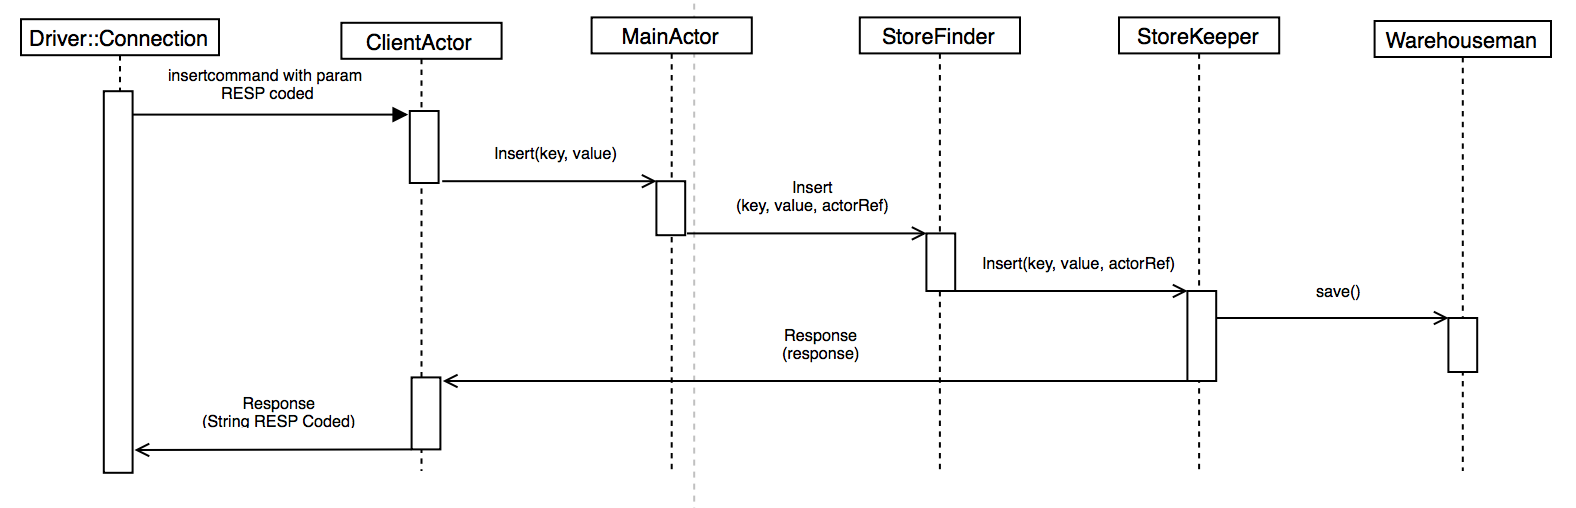
\includegraphics[width=0.9\textwidth, keepaspectratio]{img/diagrammiSequenza/esempioSave.png}
    \caption{Diagramma di sequenza - Inserimento di un item}
  \end{center}
\end{figure}

\subsection{Aggiornamento di un attore ninja}

Questo diagramma rappresenta l'interazione tra le componenti nel caso venga
effettuato un aggiornamento dei dati su un \gloss{attore} Ninja.\\
La componente \hyperref[sec:actorbase::driver::client::Connection]{actorbase::driver::client::Connection}
manda tramite \gloss{socket tcp} al \hyperref[sec:actorbase::actorsystem::clientactor::ClientActor]{actorbase::actorsystem::clientactor::ClientActor}
una stringa \hyperref[sec:RESP]{RESP} contenente il comando di inserimento \gloss{item} con
i parametri.\\
Da questo componente parte il messaggio di Insert(key, value) ad un \hyperref[sec:actorbase::actorsystem::clientactor::MainActor]{actorbase::actorsystem::clientactor::MainActor} scelto in base ad una
politica di \gloss{routing}. Il MainActor manderà un messaggio allo \hyperref[sec:actorbase::actorsystem::clientactor::StoreFinder]{actorbase::actorsystem::clientactor::StoreFinder} relativo il quale manderà un messaggio allo \hyperref[sec:actorbase::actorsystem::clientactor::StoreKeeper]{actorbase::actorsystem::clientactor::StoreKeeper} che dovrà salvarsi l'informazione
sulla propria mappa.\\
A questo punto lo Storekeeper manderà un messaggio al Ninja di tipo Update contenente la struttura dati aggiornata e successivamente manderà un
messaggio al \gloss{ClientActor} con la risposta (positiva o negativa che sia)
il quale risponderà sempre tramite \gloss{socket tcp} al \gloss{Driver} con
una stringa RESP.
Nel frattempo l'\gloss{attore} di tipo Ninja eseguirà un aggiornamento della propria struttura dati.\\
Si noti che la frequenza di aggiornamento degli attori di tipo ninja sarà
specificata tramite un parametro di configurazione del sistema.
\begin{figure}[H]
  \begin{center}
    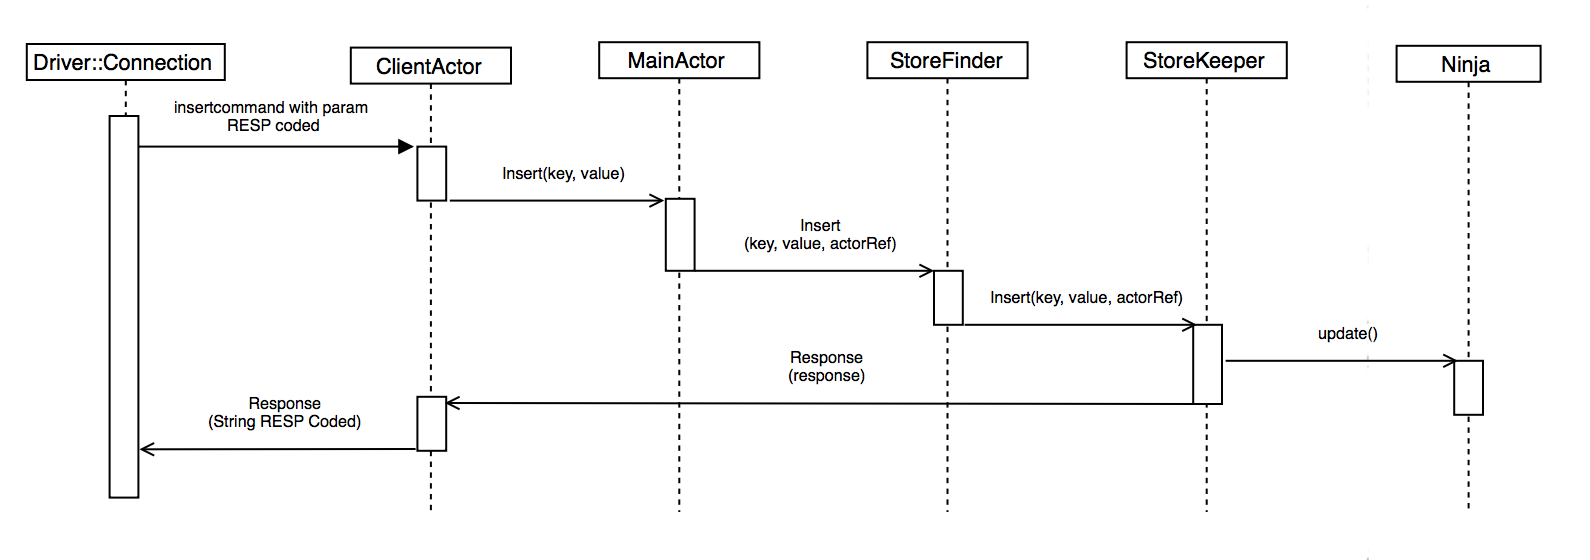
\includegraphics[width=0.9\textwidth, keepaspectratio]{img/diagrammiSequenza/esempioNinja.png}
    \caption{Diagramma di sequenza - Aggiornamento di un attore ninja}
  \end{center}
\end{figure}

\subsection{Aggiunta collaboratore (in sola lettura)}

Questo diagramma rappresenta l'interazione tra le componenti nel caso di una richiesta di autenticazione di un utente.\\
La componente \hyperref[sec:actorbase::driver::client::Connection]{actorbase::driver::client::Connection}
manda tramite \gloss{socket tcp} al \hyperref[sec:actorbase::actorsystem::clientactor::ClientActor]{actorbase::actorsystem::clientactor::ClientActor}
una stringa \hyperref[sec:RESP]{RESP} contenente il comando di aggiunta collaboratore \gloss{item} con
i parametri.\\
Da questo componente parte il messaggio di addContributor(collection, permission, username) ad un \hyperref[sec:actorbase::actorsystem::clientactor::MainActor]{actorbase::actorsystem::clientactor::MainActor} scelto in base ad una
politica di \gloss{routing}. Il MainActor manderà un messaggio allo
\hyperref[sec:actorbase::actorsystem::clientactor::StoreFinder]{actorbase::actorsystem::clientactor::StoreFinder}
relativo il quale manderà un messaggio addReadCollection(collection) allo
\hyperref[sec:actorbase::actorsystem::clientactor::UserKeeper]{actorbase::actorsystem::clientactor::UserKeeper}.
Quest'ultimo dovrà aggiungere alla mappa delle collezioni di cui l'utente
relativo ha accesso in sola lettura la collezione inviatagli.
Poi manderà al \gloss{ClientActor} un messaggio UpdateReadCollections(collection)
contenente la collezione da aggiungere.\\
Il \gloss{ClientActor} effettuerà l'aggiornamento e risponderà al \gloss{Driver}
con un messaggio che indica un esito positivo. In caso negativo resterà nello
stato attuale e manderà un messaggio al \gloss{Driver} che indica un esito
negativo.\\
Nel caso di aggiunta di un collaboratore con permessi di lettura e scrittura
l'interazione tra gli attori è la stessa con differenza di qualche messaggio
specifico.\\
\begin{figure}[H]
  \begin{center}
    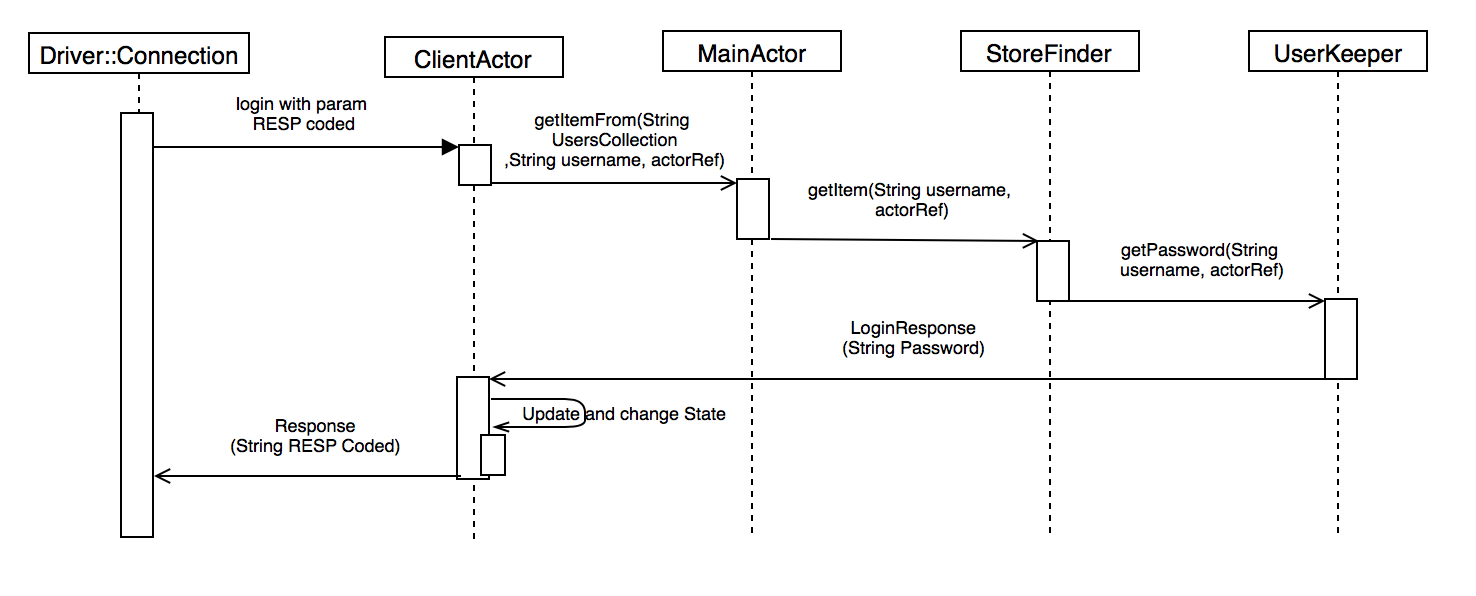
\includegraphics[width=0.9\textwidth, keepaspectratio]{img/diagrammiSequenza/esempioAuth.png}
    \caption{Diagramma di sequenza - Autenticazione}
  \end{center}
\end{figure}

\subsection{Connessione al server tramite Driver}

Questo diagramma rappresenta l'interazione tra le componenti nel caso di una richiesta di connessione al server di un utente tramite uso del \gloss{Driver}.\\Si noti che tramite utilizzo della \gloss{CLI} il diagramma sarebbe lo stesso con l'aggiunta della componente \gloss{CLI}.\\
L'utente crea un oggetto di tipo \hyperref[sec:actorbase::driver::client::ActorbaseClient]{actorbase::driver::client::ActorbaseClient}
il quale crea a sua volta un oggetto di tipo \hyperref[sec:actorbase::driver::client::Connection]{actorbase::driver::client::Connection}.
\hyperref[sec:actorbase::driver::client::Connection]{actorbase::driver::client::Connection}
instaura una connessione \gloss{tcp} con la componente
\hyperref[sec:actorbase::actorsystem::tcpserver::TCPServer]{actorbase::actorsystem::tcpserver::TCPServer} la quale crea un \gloss{attore} di tipo
\hyperref[sec:actorbase::actorsystem::clientactor::ClientActor]{actorbase::actorsystem::clientactor::ClientActor}
per gestire l'interazione tra \gloss{Driver} e server. A creazione avvenuta risponde al \gloss{Driver} il quale a cascata informa l'utente dell'avvenuta
connessione.\\
Dal diagramma possiamo vedere che le richieste successivamente inserite
dall'utente verranno gestite dal proprio \gloss{ClientActor}.\\

\begin{figure}[H]
  \begin{center}
    \includegraphics[width=0.9\textwidth, keepaspectratio]{img/diagrammiSequenza/esempioConnessione.png}
    \caption{Diagramma di sequenza - Connessione al server}
  \end{center}
\end{figure}

\section{Tracciamento}

\subsection{Tracciamento Classi-Requisiti}

\subsection{Tracciamento Requisiti-Classi}

\newpage
\appendix
\label{sec:appendice}

\newpage
\listoftables
\newpage
\listoffigures
\end{document}
